\documentclass[11pt,a4paper]{article}

\usepackage[utf8]{inputenc}
\usepackage[T1]{fontenc}
\usepackage{lmodern}
\usepackage[a4paper,margin=2.5cm]{geometry}

\usepackage{amsmath}
\usepackage{amssymb}
\usepackage{graphicx}
\usepackage{booktabs}
\usepackage{float}
\usepackage{hyperref}
\usepackage{subcaption}
\usepackage{amsmath, amssymb}
\usepackage{algorithm}
\usepackage{algpseudocode}

\title{Full-Order Model for Nonlinear RVE Homogenization with J2 Plasticity}
\date{}

\begin{document}

\maketitle

\section{Full-Order Model}

This section describes the full-order finite element model that is used to generate the dataset for the reduced-order modeling procedure. The model corresponds to a nonlinear representative volume element (RVE) undergoing small-strain elastoplastic deformation. The simulations are performed under quasi-static conditions and solved using a nonlinear finite element formulation.

The objective of the present work is to construct a nonlinear projection-based reduced-order model capable of approximating the microscopic displacement field while preserving the accuracy of the homogenized macroscopic response of the RVE.

\subsection{Representative Volume Element}

The computational domain corresponds to a two-dimensional representative volume element containing a central void. The geometry is discretized with a finite element mesh composed of triangular elements. The mesh used in the present simulations contains

\begin{itemize}
\item 1058 nodes
\item 486 elements
\end{itemize}

The problem is solved under plane stress conditions. The geometry and the discretization of the RVE are illustrated in Figure~\ref{fig:rve_mesh}.

\begin{figure}[H]
\centering
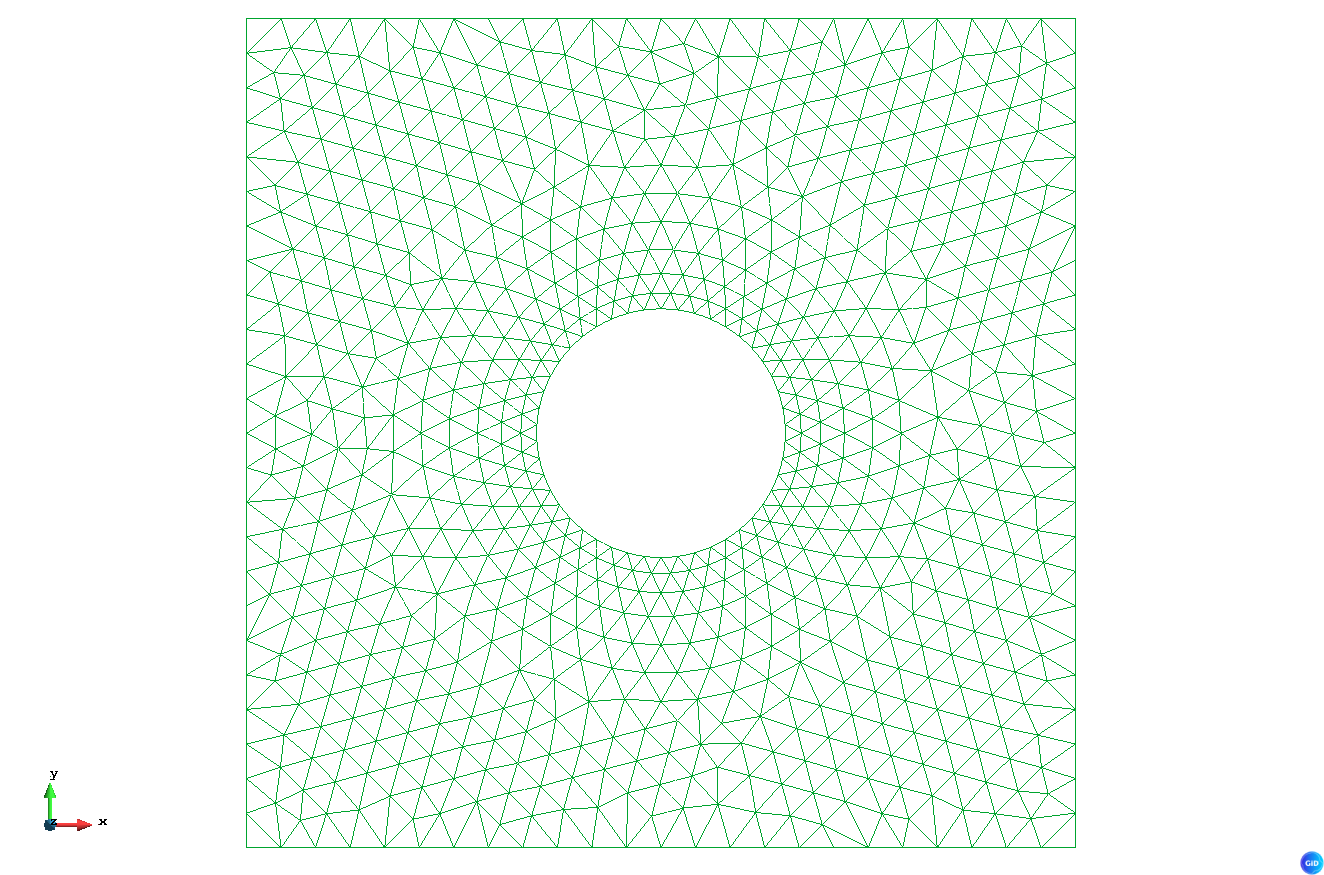
\includegraphics[width=0.65\textwidth]{MeshAndGeometry.png}
\caption{Finite element discretization of the representative volume element.}
\label{fig:rve_mesh}
\end{figure}

\subsection{Governing Mechanical Model}

The RVE is governed by a small-strain elastoplastic constitutive model of J2 type with isotropic hardening. The material exhibits an elastic response at small stresses and undergoes plastic deformation once the yield condition is reached.

The constitutive model is implemented at the integration points of the finite elements. During the simulation the constitutive law updates the local stress state and the associated internal variables according to the strain history experienced by each integration point.

In the present work the details of the constitutive integration algorithm are not discussed, since the focus is placed on the reduced-order modeling strategy rather than on the constitutive formulation itself.

\subsection{Finite Element Discretization}

The displacement field of the RVE is discretized using finite element shape functions. After spatial discretization, the mechanical equilibrium problem leads to a nonlinear algebraic system of equations of the form

\begin{equation}
\mathbf{R}(\mathbf{u},\mathbf{z}) = \mathbf{0}
\end{equation}

where $\mathbf{u}$ denotes the vector of nodal displacements and $\mathbf{R}$ is the nonlinear residual vector representing the imbalance between internal and external forces.

The vector $\mathbf{z}$ represents the collection of internal variables associated with the constitutive model at the integration points of the finite elements. These variables describe the internal state of the material and evolve during the loading process. As a consequence, the equilibrium equations depend not only on the current displacement field but also on the internal state of the material.

The nonlinear system is solved using a Newton-type iterative scheme. At each iteration the following linear system is solved

\begin{equation}
\mathbf{K}(\mathbf{u}_k,\mathbf{z}_k)\Delta \mathbf{u}
=
-\mathbf{R}(\mathbf{u}_k,\mathbf{z}_k)
\end{equation}

where $\mathbf{K}(\mathbf{u}_k,\mathbf{z}_k)$ is the tangent stiffness matrix evaluated at the current configuration and internal state of the material.

The displacement field is updated according to

\begin{equation}
\mathbf{u}_{k+1} = \mathbf{u}_k + \Delta \mathbf{u}.
\end{equation}

During the Newton iterations, the constitutive model updates the internal variables consistently with the current strain state.
\subsection{Macroscopic Loading Conditions}

The RVE is subjected to macroscopic strain-controlled loading. The macroscopic deformation is imposed through affine displacement boundary conditions applied on the external boundary of the RVE.

Let the macroscopic strain tensor be

\begin{equation}
\boldsymbol{\varepsilon}^{M} =
\begin{bmatrix}
\varepsilon_{xx}^{M} & \varepsilon_{xy}^{M} \\
\varepsilon_{xy}^{M} & \varepsilon_{yy}^{M}
\end{bmatrix}.
\end{equation}

The displacement imposed at a boundary point with position vector $\mathbf{x}$ is given by the affine relation

\begin{equation}
\mathbf{u}(\mathbf{x}) = \boldsymbol{\varepsilon}^{M}\mathbf{x}.
\end{equation}

This boundary condition enforces consistency between the microscopic deformation of the RVE and the prescribed macroscopic strain.

In the present study we consider uniaxial macroscopic strain histories in which the dominant component of the loading tensor is $\varepsilon_{xx}^{M}$. The loading path therefore evolves according to a sequence of strain increments

\begin{equation}
\Delta \varepsilon_{xx}^{M}.
\end{equation}

The sign of this increment plays an important role in the subsequent modeling strategy, since positive and negative loading directions may correspond to different deformation responses of the system.

\subsection{Homogenized Macroscopic Response}

Once the microscopic equilibrium problem has been solved, the effective macroscopic stress associated with the RVE is obtained through a volume average of the microscopic stress field over the domain.

The homogenized stress tensor is defined as

\begin{equation}
\boldsymbol{\sigma}^{M}
=
\frac{1}{|\Omega|}
\int_{\Omega}
\boldsymbol{\sigma}(\mathbf{x})\, d\Omega .
\end{equation}

This quantity represents the macroscopic stress response associated with the imposed macroscopic strain.

The pair
\[
\left(
\boldsymbol{\varepsilon}^{M},
\boldsymbol{\sigma}^{M}
\right)
\]

defines the effective constitutive response of the RVE.

During the full-order simulations, the imposed macroscopic strain and the corresponding homogenized stress are recorded at every loading increment. These quantities are later used to evaluate the predictive capability of the reduced-order model, which must reproduce not only the displacement field but also the macroscopic stress response obtained from the homogenization procedure.

\section{Training Dataset for the Linear Projection-Based Reduced Model}

Before constructing a nonlinear reduced model, we first build a linear projection-based reduced-order model. The construction of this linear reduced space requires the generation of displacement snapshots obtained from the full-order model.

\subsection{Loading Trajectories}

Two loading trajectories are used to generate the snapshot dataset. Both trajectories correspond to uniaxial macroscopic strain paths applied to the RVE. One trajectory corresponds to monotonic loading in the positive direction, while the second trajectory corresponds to loading in the opposite direction.

Let the macroscopic strain tensor be

\begin{equation}
\boldsymbol{\varepsilon}^{M}(t)
=
\begin{bmatrix}
\varepsilon_{xx}^{M}(t) & 0 \\
0 & 0
\end{bmatrix}.
\end{equation}

The two training trajectories correspond to monotonic evolutions of the component $\varepsilon_{xx}^{M}$

\begin{equation}
\text{Trajectory 1:} \qquad
\varepsilon_{xx}^{M}(t) \text{ increases monotonically from } 0 \text{ to } \varepsilon_{\max},
\end{equation}

\begin{equation}
\text{Trajectory 2:} \qquad
\varepsilon_{xx}^{M}(t) \text{ decreases monotonically from } 0 \text{ to } -\varepsilon_{\max}.
\end{equation}

Each trajectory starts from the undeformed configuration

\begin{equation}
\boldsymbol{\varepsilon}^{M} = \mathbf{0}
\end{equation}

and evolves through a sequence of strain increments

\begin{equation}
\Delta \varepsilon_{xx}^{M}.
\end{equation}

At each loading increment the nonlinear equilibrium problem of the full-order model is solved.

During the simulation the microscopic displacement field and the homogenized macroscopic response are stored.

\subsection{Snapshot Collection}

Let $\mathbf{u}_i$ denote the nodal displacement vector obtained at loading step $i$ of the simulation. These vectors represent the microscopic displacement solutions associated with the different states of the RVE along the loading trajectories.

The collection of displacement snapshots can therefore be written as

\begin{equation}
\mathbf{u}_1,\mathbf{u}_2,\dots,\mathbf{u}_{N_s} .
\end{equation}

These snapshots are assembled into the snapshot matrix

\begin{equation}
\mathbf{S}
=
\begin{bmatrix}
\mathbf{u}_1 &
\mathbf{u}_2 &
\cdots &
\mathbf{u}_{N_s}
\end{bmatrix}.
\end{equation}

This matrix contains the displacement solutions generated by the full-order model for the two loading trajectories. The snapshot matrix constitutes the dataset used to construct the reduced basis for the projection-based reduced-order model.

\subsection{Stored Homogenized Quantities}

In addition to the displacement field, the homogenized stress and strain associated with the RVE are also recorded at each loading step.

Let

\begin{equation}
\boldsymbol{\varepsilon}^{M}_i
\end{equation}

and

\begin{equation}
\boldsymbol{\sigma}^{M}_i
\end{equation}

denote the homogenized strain and stress tensors obtained at loading step $i$. These quantities define the effective macroscopic stress--strain response of the RVE along the loading trajectories.

The evolution of the homogenized stress as a function of the imposed macroscopic strain will later be used to assess the predictive capability of the reduced-order model.

\subsection{Examples of Full-Order Solutions}

Figures~\ref{fig:traj_tension} and \ref{fig:traj_compression} illustrate the displacement field obtained at the final step of the two training trajectories. These solutions correspond to the largest macroscopic strain reached during each loading path.

\begin{figure}[H]
\centering
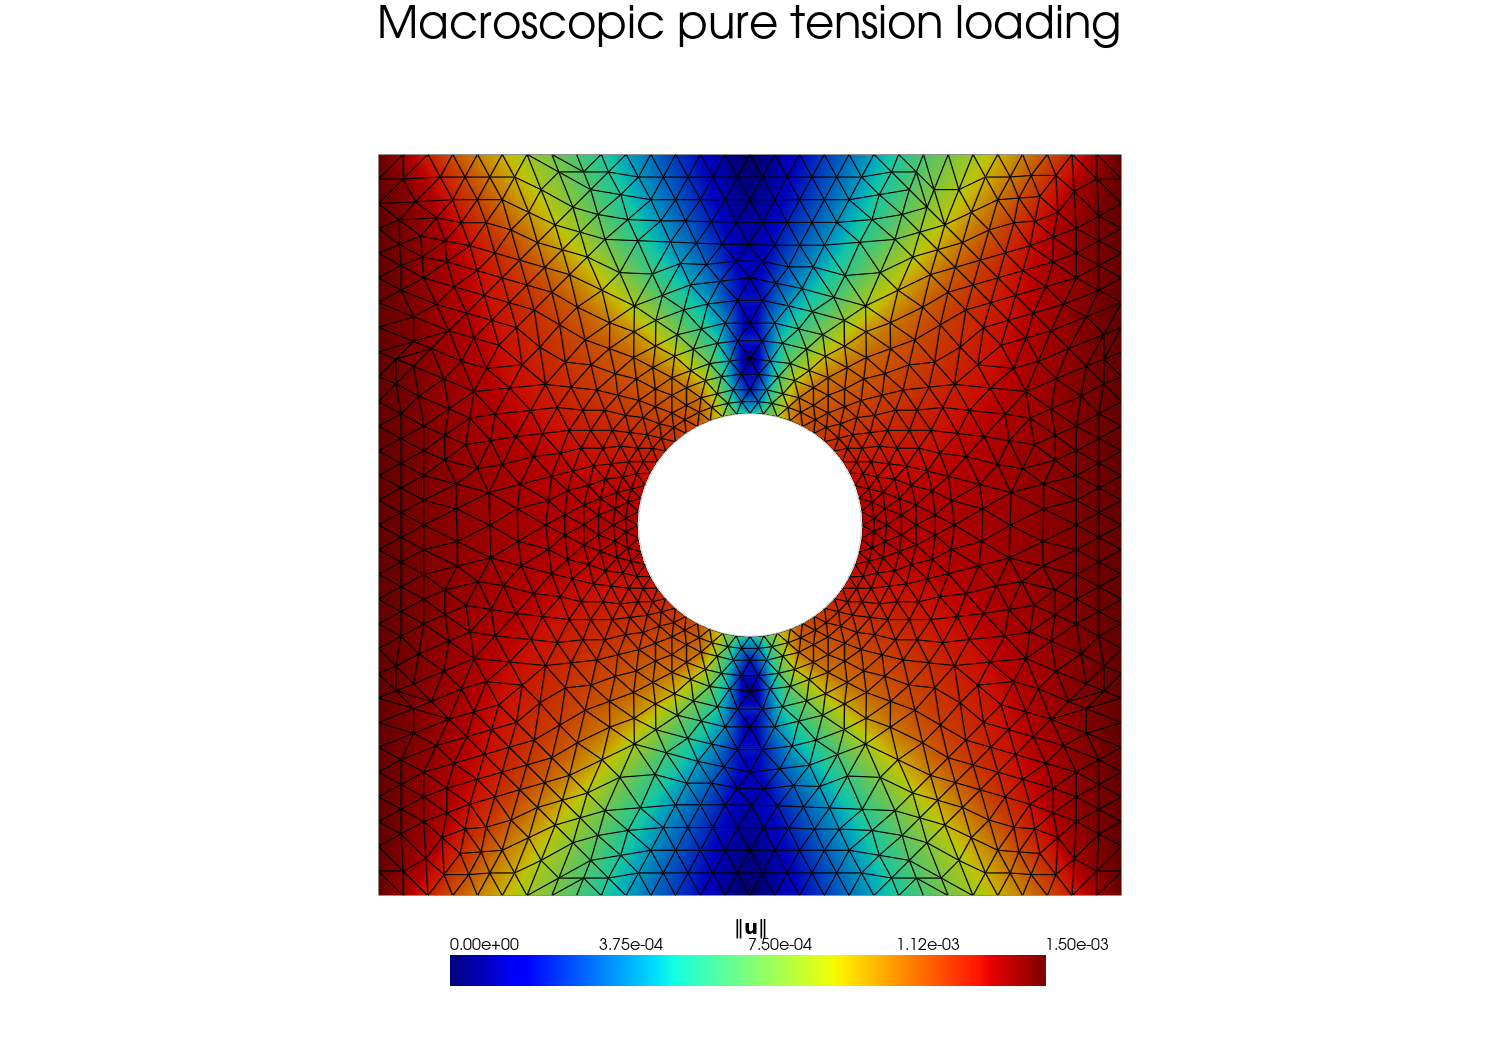
\includegraphics[width=0.65\textwidth]{trajectory_positive_solution.png}
\caption{Displacement field obtained at the final step of the macroscopic pure tension loading trajectory.}
\label{fig:traj_tension}
\end{figure}

\begin{figure}[H]
\centering
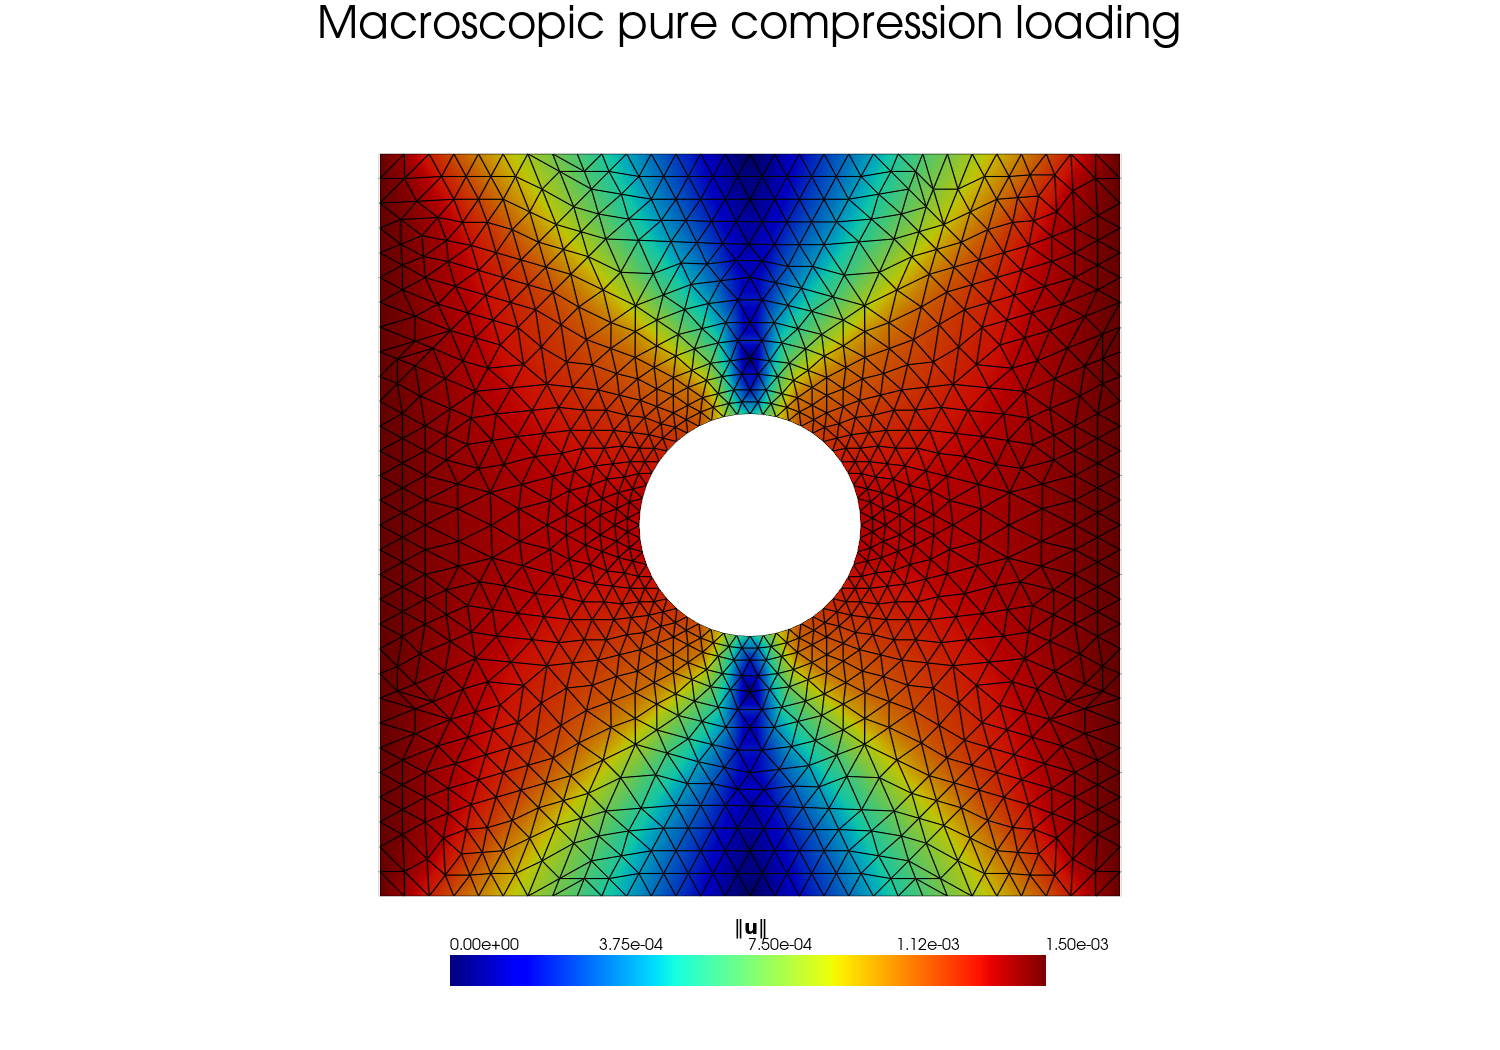
\includegraphics[width=0.65\textwidth]{trajectory_negative_solution.png}
\caption{Displacement field obtained at the final step of the macroscopic pure compression loading trajectory.}
\label{fig:traj_compression}
\end{figure}

These full-order solutions provide the information required to construct a reduced linear subspace in which the reduced-order model will be formulated.

\subsection{Homogenized Stress--Strain Response}

Figures~\ref{fig:hom_tension} and \ref{fig:hom_compression} show the homogenized macroscopic stress--strain response obtained from the full-order simulations used to generate the training dataset.

\begin{figure}[H]
\centering
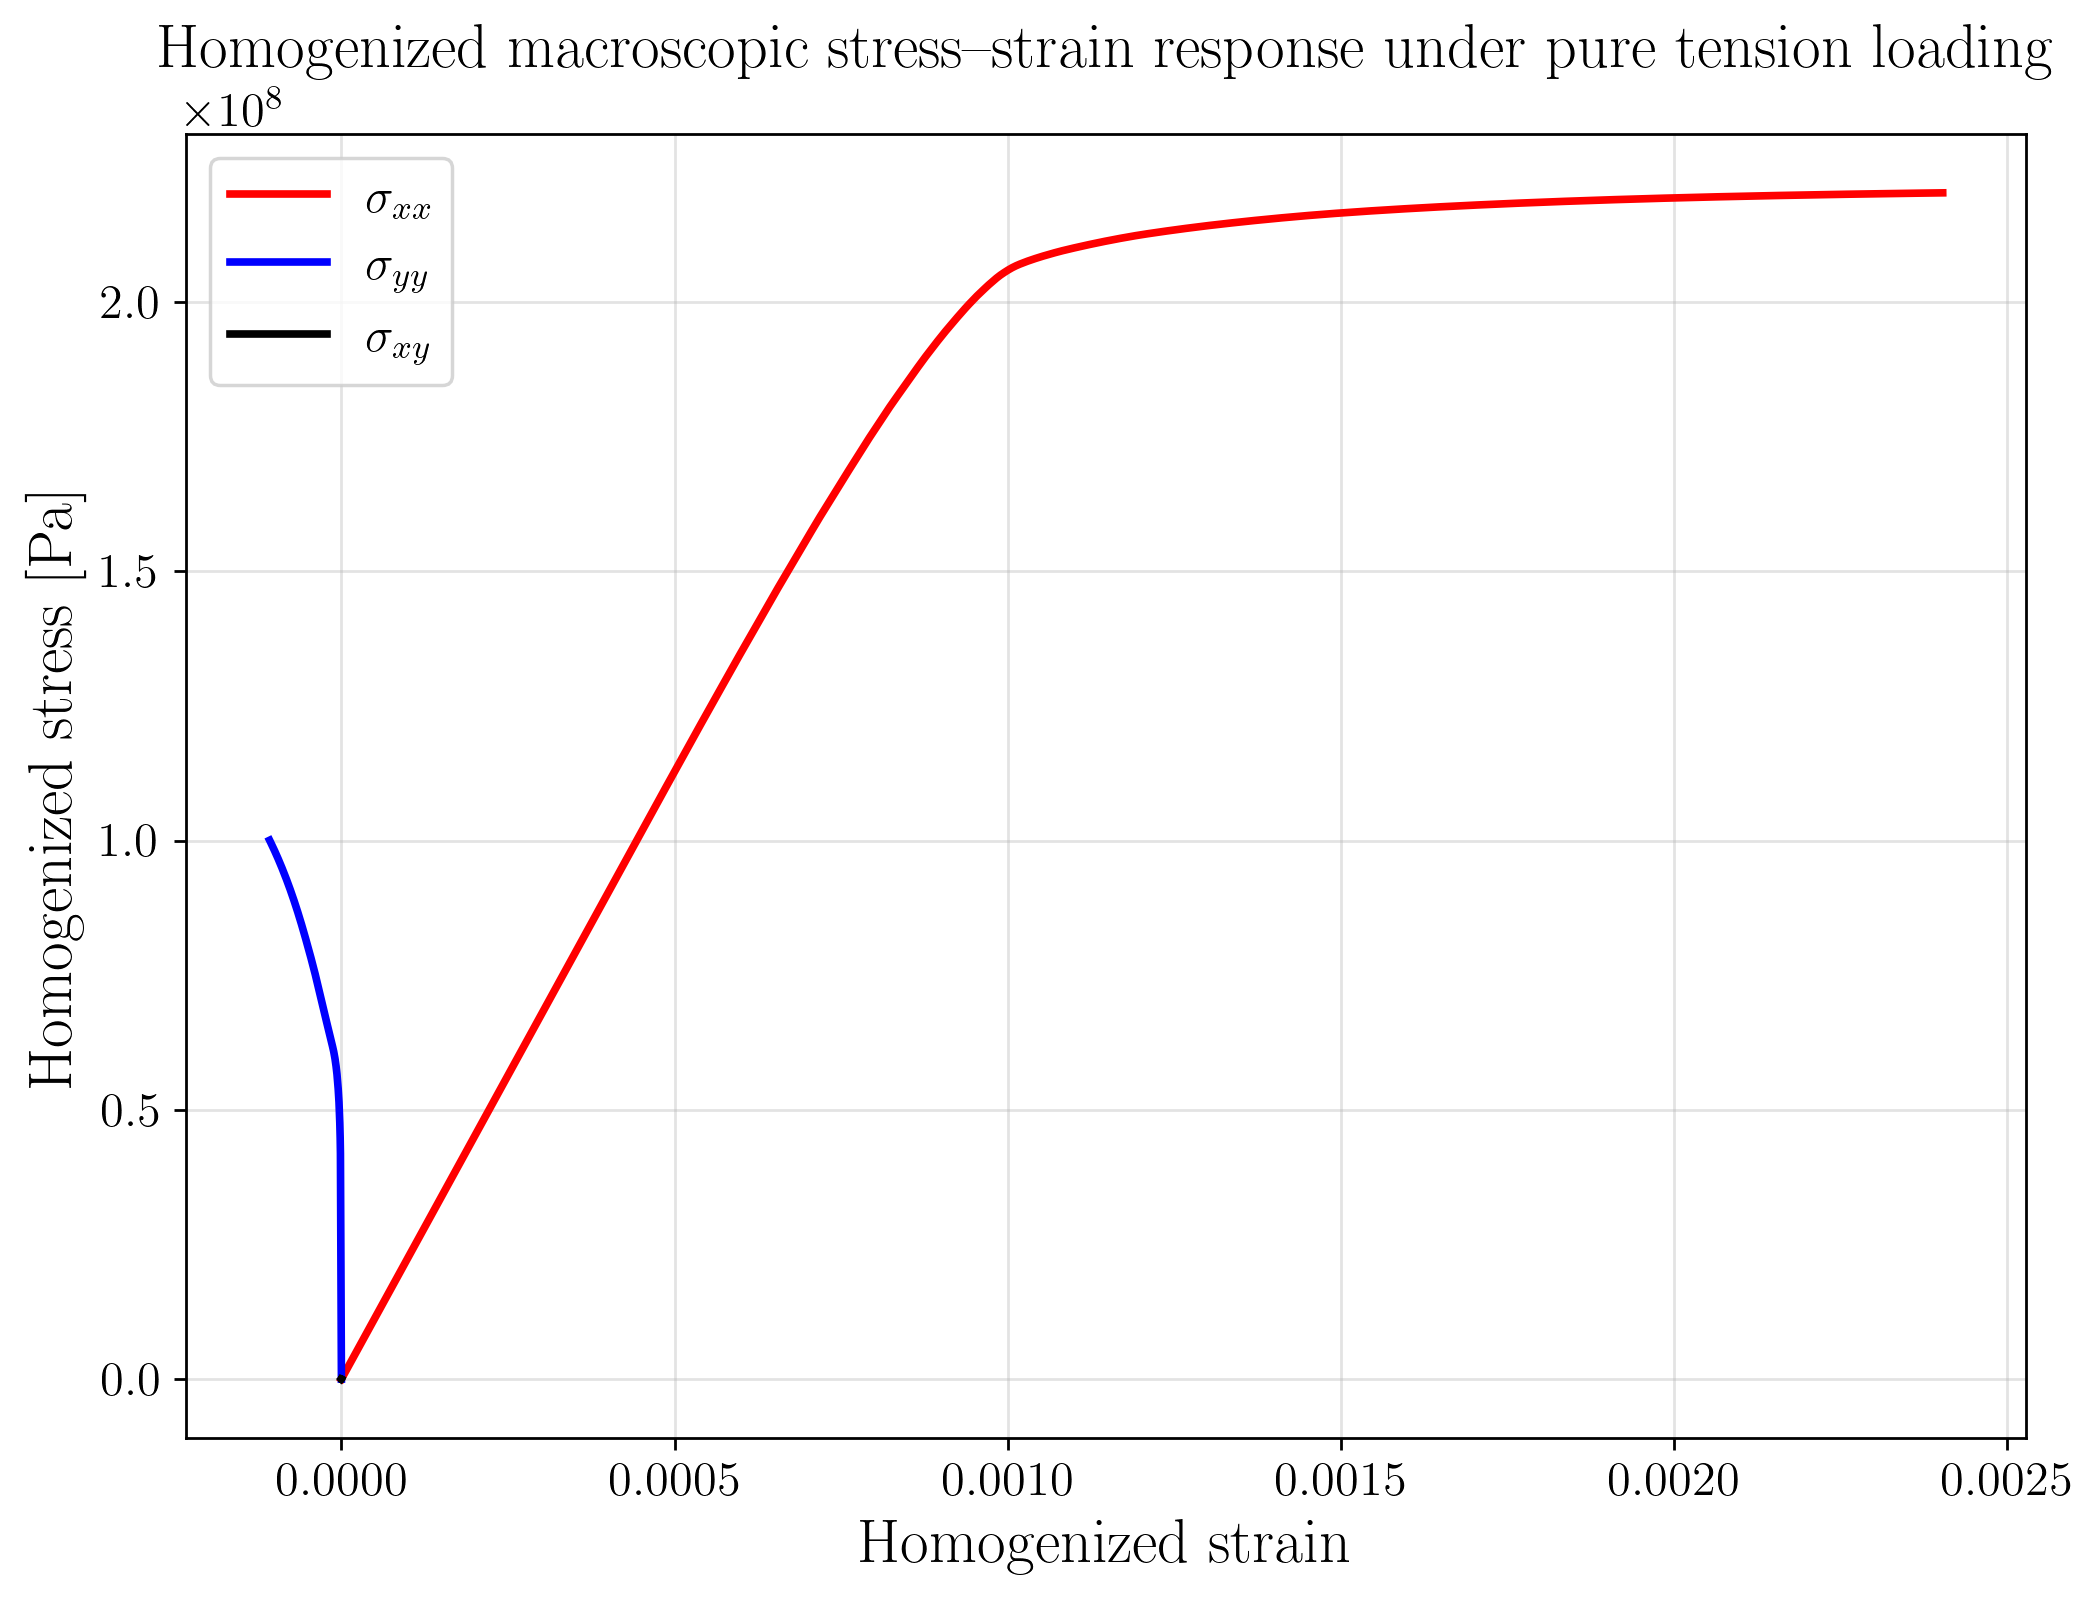
\includegraphics[width=0.7\textwidth]{stress_strain_tension.png}
\caption{Homogenized macroscopic stress--strain response obtained under macroscopic pure tension loading.}
\label{fig:hom_tension}
\end{figure}

\begin{figure}[H]
\centering
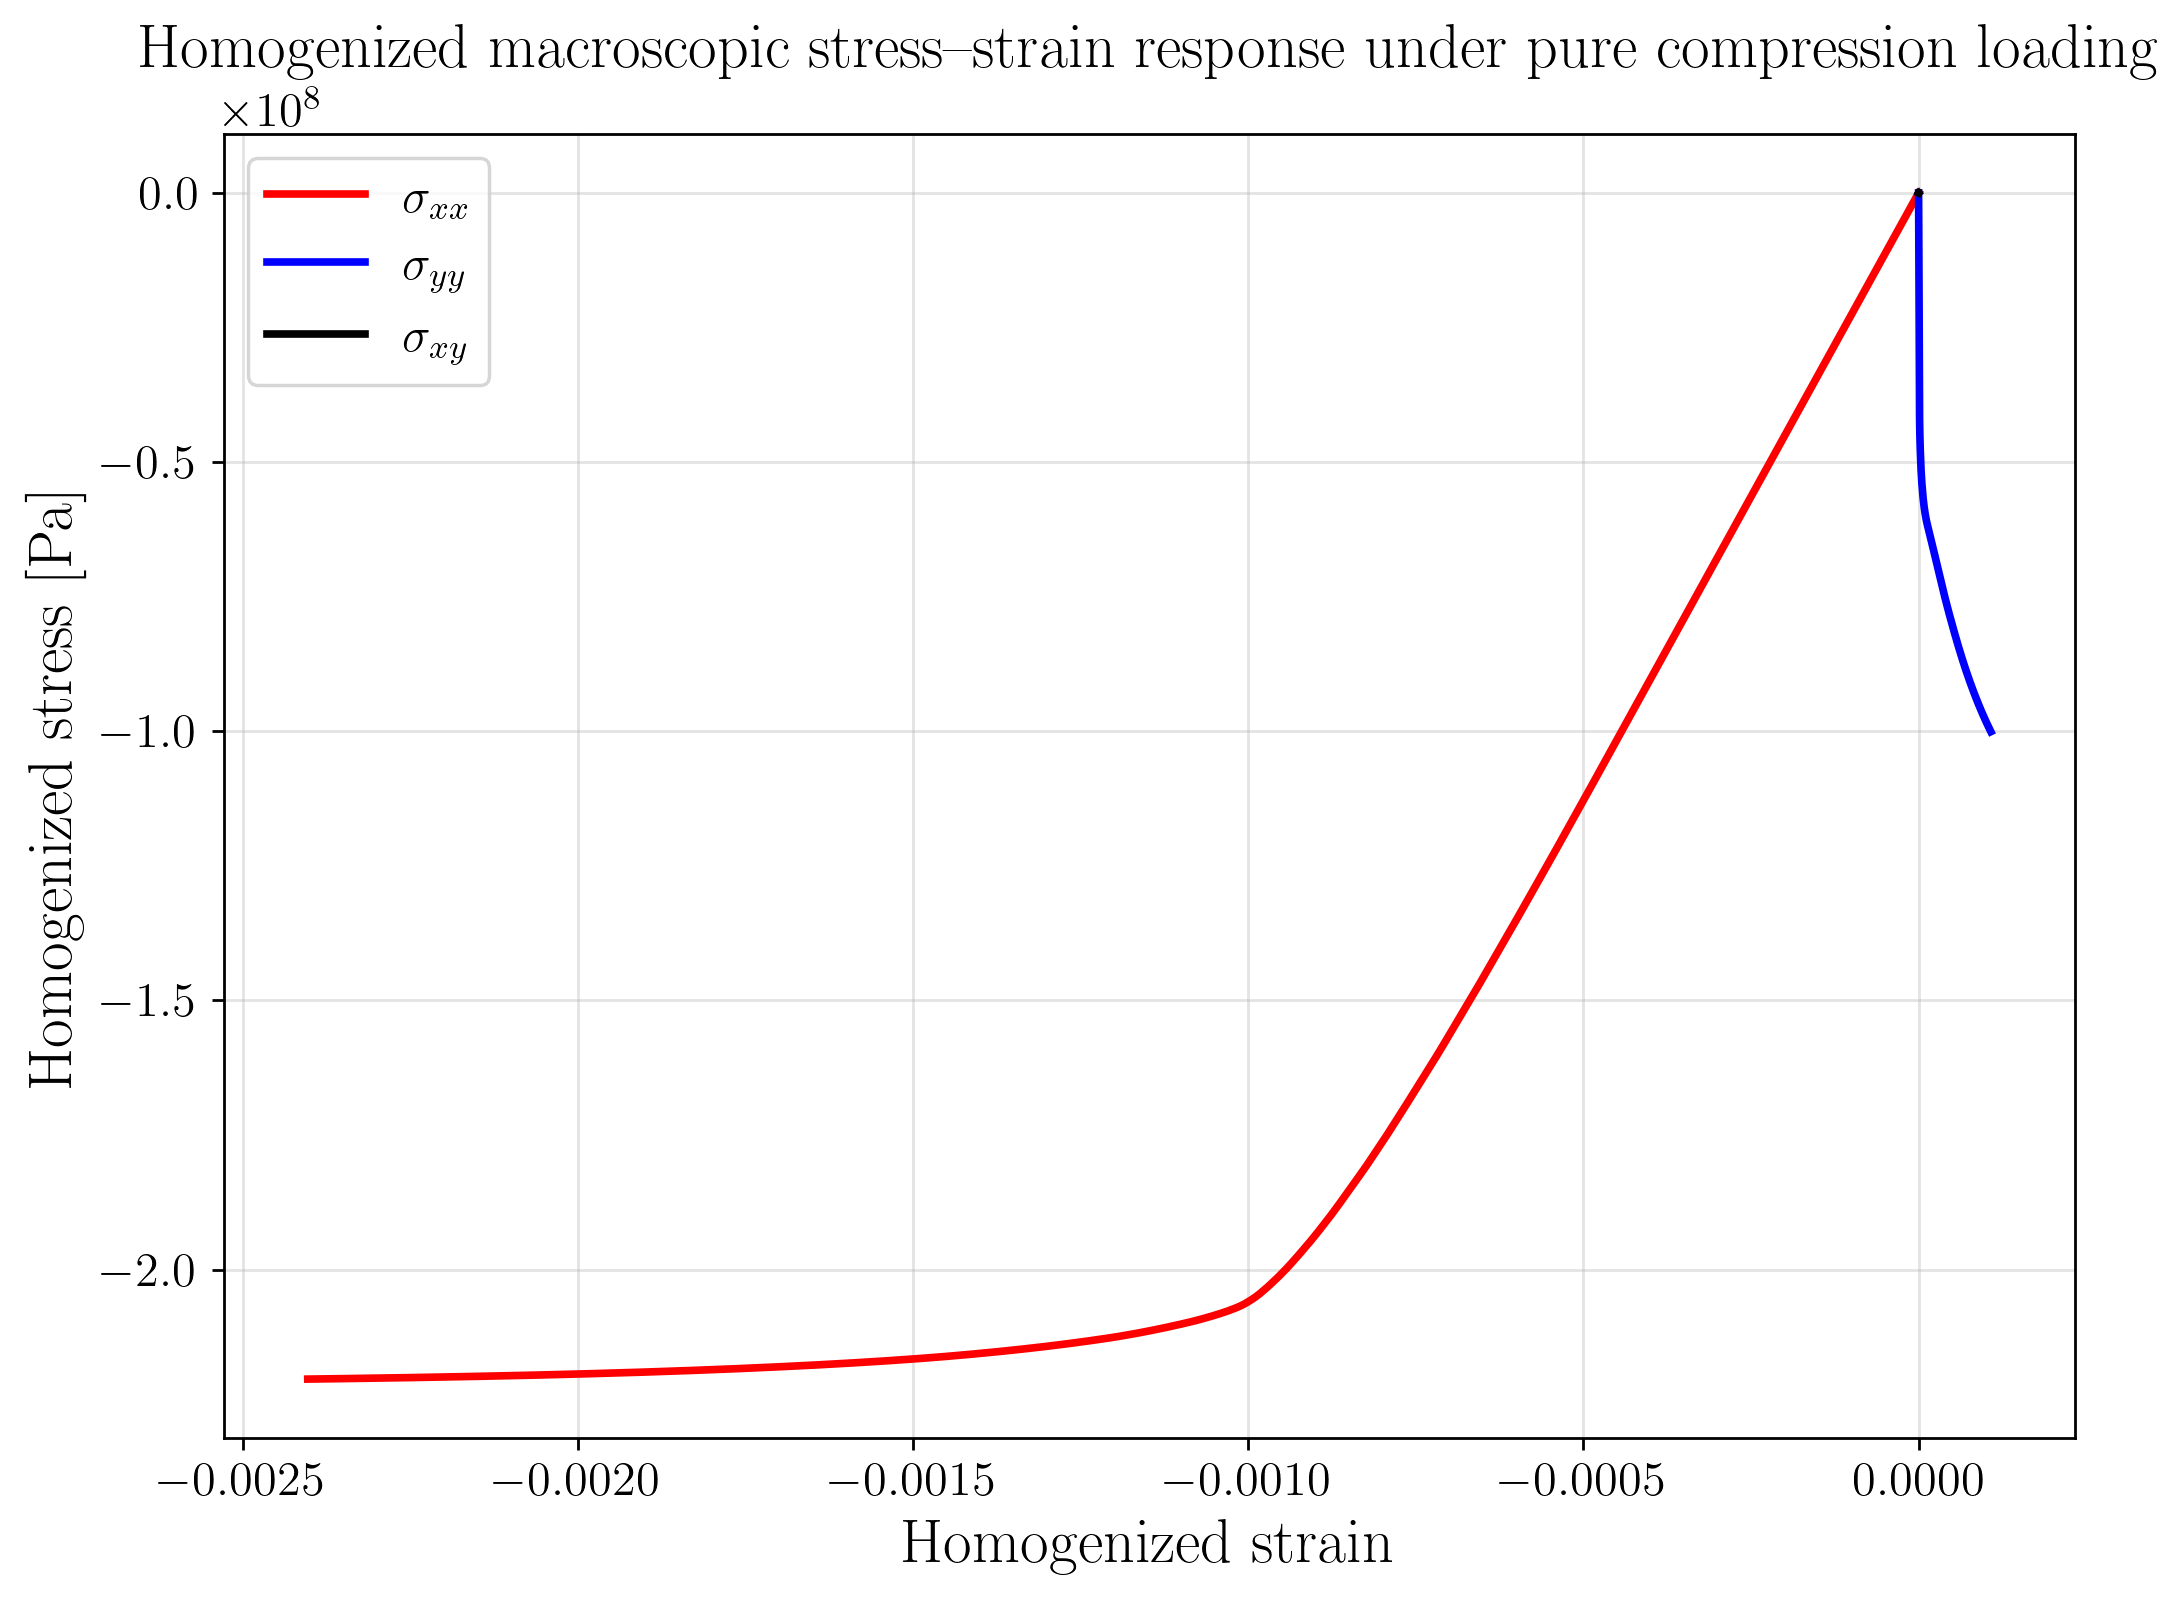
\includegraphics[width=0.7\textwidth]{stress_strain_compression.png}
\caption{Homogenized macroscopic stress--strain response obtained under macroscopic pure compression loading.}
\label{fig:hom_compression}
\end{figure}

The nonlinear behavior observed in these curves reflects the elastoplastic response of the RVE under the prescribed macroscopic loading conditions.
\section{Proper Orthogonal Decomposition for the Linear Projection-Based Reduced Model}

This section describes the construction of the reduced linear subspace used to define the projection-based reduced-order model. The reduced basis is obtained from the displacement snapshots generated by the full-order simulations presented in the previous section.

The construction is based on Proper Orthogonal Decomposition (POD). However, rather than building a single basis directly from all displacement snapshots, the procedure distinguishes between an initial elastic contribution and a subsequent plastic contribution. This separation is introduced in order to capture more clearly the structure of the solution manifold, where the early response is dominated by elastic deformations and the later response contains additional nonlinear effects associated with plastic evolution.

\subsection{Free and Dirichlet Degrees of Freedom}

The finite element degrees of freedom are first partitioned into free and Dirichlet sets. Let the full displacement vector be denoted by

\begin{equation}
\mathbf{u} =
\begin{bmatrix}
\mathbf{u}_f \\
\mathbf{u}_d
\end{bmatrix},
\end{equation}

where $\mathbf{u}_f$ contains the free degrees of freedom and $\mathbf{u}_d$ contains the prescribed Dirichlet degrees of freedom.

Since the loading is imposed through affine displacement boundary conditions, the Dirichlet contribution is represented separately from the reduced approximation of the free part. The reduced basis is therefore constructed only for the free degrees of freedom.

\subsection{Snapshot Matrix for the Free Degrees of Freedom}

From each full-order displacement snapshot $\mathbf{u}_i$, the corresponding restriction to the free degrees of freedom is extracted,

\begin{equation}
\mathbf{u}_{f,i} \in \mathbb{R}^{n_f},
\end{equation}

where $n_f$ denotes the number of free degrees of freedom.

The snapshot matrix associated with the free part is then written as

\begin{equation}
\mathbf{S}_f
=
\begin{bmatrix}
\mathbf{u}_{f,1} &
\mathbf{u}_{f,2} &
\cdots &
\mathbf{u}_{f,N_s}
\end{bmatrix}
\in
\mathbb{R}^{n_f \times N_s}.
\end{equation}

This matrix contains all the displacement information that will be used to construct the reduced subspace for the unknown degrees of freedom.

\subsection{Reference Stiffness Matrix and Energy Inner Product}

The reduced basis vectors are later orthonormalized with respect to an energy-based metric induced by a reference stiffness matrix, rather than the standard Euclidean inner product.

Let $\mathbf{K}_{ff}^{\mathrm{ref}}$ denote the free-free block of the reference tangent stiffness matrix assembled at the undeformed configuration. This matrix defines the bilinear form

\begin{equation}
\langle \mathbf{v}, \mathbf{w} \rangle_{\mathbf{K}}
=
\mathbf{v}^{T}\mathbf{K}_{ff}^{\mathrm{ref}}\mathbf{w}.
\end{equation}

This inner product provides a mechanically meaningful notion of orthogonality and normalization for the reduced basis vectors.

\subsection{Elastic and Plastic Contributions to the Reduced Basis}

The reduced basis is constructed in two stages.

First, an elastic subspace is extracted from the subset of snapshots identified as elastic. These correspond to the loading steps for which no integration point in the RVE has yet activated plastic evolution. Let the corresponding elastic snapshot matrix be denoted by

\begin{equation}
\mathbf{S}_f^{\mathrm{el}}
=
\begin{bmatrix}
\mathbf{u}_{f,1}^{\mathrm{el}} &
\mathbf{u}_{f,2}^{\mathrm{el}} &
\cdots &
\mathbf{u}_{f,N_{\mathrm{el}}}^{\mathrm{el}}
\end{bmatrix}.
\end{equation}

A singular value decomposition of this matrix is then performed,

\begin{equation}
\mathbf{S}_f^{\mathrm{el}}
=
\mathbf{U}^{\mathrm{el}}
\mathbf{\Sigma}^{\mathrm{el}}
\left(\mathbf{V}^{\mathrm{el}}\right)^T .
\end{equation}

After truncation, the leading left singular vectors define the initial elastic basis, denoted by

\begin{equation}
\mathbf{\Phi}_{f}^{\mathrm{el}} \in \mathbb{R}^{n_f \times r_{\mathrm{el}}}.
\end{equation}

Second, the plastic contribution is extracted from the components of the full snapshots that are not represented by the elastic subspace. For each free displacement snapshot $\mathbf{u}_{f,i}$, its projection onto the elastic space is first computed in the stiffness-induced inner product. The corresponding residual is then given by

\begin{equation}
\mathbf{r}_{f,i}^{\mathrm{pl}}
=
\mathbf{u}_{f,i}
-
\mathbf{\Phi}_{f}^{\mathrm{el}}
\mathbf{q}_{i}^{\mathrm{el}},
\end{equation}

where the elastic projection coefficients are defined using the stiffness-induced inner product as

\begin{equation}
\mathbf{q}_{i}^{\mathrm{el}}
=
\left(\mathbf{\Phi}_{f}^{\mathrm{el}}\right)^T
\mathbf{K}_{ff}^{\mathrm{ref}}
\mathbf{u}_{f,i}.
\end{equation}

These residual vectors are assembled into a second snapshot matrix,

\begin{equation}
\mathbf{S}_f^{\mathrm{pl}}
=
\begin{bmatrix}
\mathbf{r}_{f,1}^{\mathrm{pl}} &
\mathbf{r}_{f,2}^{\mathrm{pl}} &
\cdots &
\mathbf{r}_{f,N_s}^{\mathrm{pl}}
\end{bmatrix}.
\end{equation}

A second singular value decomposition is then applied to this residual matrix,

\begin{equation}
\mathbf{S}_f^{\mathrm{pl}}
=
\mathbf{U}^{\mathrm{pl}}
\mathbf{\Sigma}^{\mathrm{pl}}
\left(\mathbf{V}^{\mathrm{pl}}\right)^T ,
\end{equation}

and the leading modes define a plastic basis

\begin{equation}
\mathbf{\Phi}_{f}^{\mathrm{pl}} \in \mathbb{R}^{n_f \times r_{\mathrm{pl}}}.
\end{equation}

The final reduced basis for the free degrees of freedom is obtained by concatenation,

\begin{equation}
\mathbf{\Phi}_f
=
\begin{bmatrix}
\mathbf{\Phi}_{f}^{\mathrm{el}} &
\mathbf{\Phi}_{f}^{\mathrm{pl}}
\end{bmatrix}.
\end{equation}

\subsection{Stiffness-Orthonormal Reduced Basis}

The elastic and plastic basis vectors are orthonormalized with respect to the inner product induced by $\mathbf{K}_{ff}^{\mathrm{ref}}$. As a result, the final reduced basis satisfies

\begin{equation}
\mathbf{\Phi}_f^{T}\mathbf{K}_{ff}^{\mathrm{ref}}\mathbf{\Phi}_f
=
\mathbf{I},
\end{equation}

and, in particular, the elastic and plastic blocks are mutually orthogonal in the same metric,

\begin{equation}
\left(\mathbf{\Phi}_{f}^{\mathrm{el}}\right)^T
\mathbf{K}_{ff}^{\mathrm{ref}}
\mathbf{\Phi}_{f}^{\mathrm{pl}}
=
\mathbf{0}.
\end{equation}

This construction guarantees that the reduced coordinates are defined in an energy-consistent basis and that the plastic correction space complements, rather than duplicates, the elastic contribution.

\subsection{Dirichlet Lifting Representation}

The prescribed boundary displacement is represented separately through a low-dimensional affine map acting on the macroscopic strain components. Let

\begin{equation}
\mathbf{\Phi}_d \in \mathbb{R}^{n_d \times 3}
\end{equation}

denote the matrix that maps the macroscopic strain components to the Dirichlet degrees of freedom, where $n_d$ is the number of prescribed degrees of freedom. The three columns correspond to the independent components of the macroscopic strain tensor $(\varepsilon_{xx}^M,\varepsilon_{yy}^M,\varepsilon_{xy}^M)$.

This matrix provides the centered affine boundary displacement associated with the imposed macroscopic loading. It is not obtained from POD, but directly from the form of the boundary conditions.

\subsection{Linear Reduced Representation}

Using the previous ingredients, the full displacement vector is approximated by combining the free reduced approximation with the affine Dirichlet contribution. In block form, the reduced approximation reads

\begin{equation}
\mathbf{u}
\approx
\begin{bmatrix}
\mathbf{\Phi}_f \mathbf{q} \\
\mathbf{\Phi}_d \boldsymbol{\varepsilon}^{M}
\end{bmatrix},
\end{equation}

where $\mathbf{q} \in \mathbb{R}^{r}$ denotes the reduced coordinates and

\begin{equation}
r = r_{\mathrm{el}} + r_{\mathrm{pl}}
\end{equation}

is the total dimension of the reduced space.

In the present case the truncation procedure yields

\begin{equation}
r_{\mathrm{el}} = 1,
\qquad
r_{\mathrm{pl}} = 7,
\end{equation}

so that the final reduced dimension is

\begin{equation}
r = 8 .
\end{equation}

This approximation defines the linear subspace on which the first projection-based reduced-order model is built.

\section{Validation of the Linear Projection-Based Reduced-Order Model}

Once the reduced basis has been constructed, a first projection-based reduced-order model is defined on the linear subspace introduced in the previous section. This linear PROM serves as the baseline reduced model and allows us to assess how much of the nonlinear RVE response can already be captured with a very compact linear approximation.

\subsection{Reduced Equilibrium Problem}

The linear reduced-order model is obtained by substituting the reduced approximation into the full-order equilibrium equations and projecting the resulting residual onto the reduced space.

Let the reduced approximation of the free degrees of freedom be written as

\begin{equation}
\mathbf{u}_f \approx \mathbf{\Phi}_f \mathbf{q},
\end{equation}

where $\mathbf{\Phi}_f \in \mathbb{R}^{n_f \times r}$ is the reduced basis and $\mathbf{q} \in \mathbb{R}^{r}$ denotes the reduced coordinates.

The corresponding reduced nonlinear equilibrium equations are written as

\begin{equation}
\mathbf{r}(\mathbf{q})
=
\mathbf{\Phi}_f^T
\mathbf{R}_f\!\left(\mathbf{\Phi}_f \mathbf{q},\mathbf{z},\boldsymbol{\varepsilon}^{M}\right)
=
\mathbf{0},
\end{equation}

where $\mathbf{R}_f$ denotes the restriction of the full-order residual to the free degrees of freedom.

The associated reduced tangent matrix is given by

\begin{equation}
\mathbf{K}_r(\mathbf{q})
=
\mathbf{\Phi}_f^T
\mathbf{K}_{ff}
\!\left(\mathbf{\Phi}_f \mathbf{q},\mathbf{z},\boldsymbol{\varepsilon}^{M}\right)
\mathbf{\Phi}_f.
\end{equation}

At each nonlinear iteration, the reduced correction is obtained from

\begin{equation}
\mathbf{K}_r(\mathbf{q}_k)\,\Delta \mathbf{q}
=
-
\mathbf{r}(\mathbf{q}_k),
\end{equation}

and the reduced coordinates are updated according to

\begin{equation}
\mathbf{q}_{k+1} = \mathbf{q}_k + \Delta \mathbf{q}.
\end{equation}

The resulting reduced solution is then lifted back to the full-order space through the reduced basis for the free degrees of freedom together with the affine Dirichlet contribution.

\subsection{Validation Trajectory}

The predictive capability of the linear reduced-order model is assessed on a loading trajectory that is different from the two monotonic trajectories used during training. The validation path contains several loading reversals and therefore probes states that are not explicitly contained in the original training trajectories.

This test is especially relevant because the reduced basis was constructed from only two monotonic uniaxial paths, yet the reduced model is asked to approximate a richer non-monotonic response. The purpose of this validation is therefore to determine whether such a compact linear reduced space is already sufficient to reproduce the microscopic and macroscopic response of the RVE with good accuracy.

\subsection{Comparison Metrics}

The linear reduced-order model is compared against the full-order model using relative $\ell^2$ errors computed over the complete time history of the validation simulation.

Let $\mathbf{U}^{\mathrm{FOM}}$ and $\mathbf{U}^{\mathrm{PROM}}$ denote the full histories of the displacement field, and similarly let
\[
\mathbf{E}^{\mathrm{FOM}},\;\mathbf{E}^{\mathrm{PROM}},
\qquad
\mathbf{\Sigma}^{\mathrm{FOM}},\;\mathbf{\Sigma}^{\mathrm{PROM}}
\]
denote the histories of homogenized strain and homogenized stress, respectively. The relative error is computed as

\begin{equation}
\epsilon_{\mathbf{A}}
=
\frac{
\left\|
\mathbf{A}^{\mathrm{PROM}} - \mathbf{A}^{\mathrm{FOM}}
\right\|_2
}{
\left\|
\mathbf{A}^{\mathrm{FOM}}
\right\|_2
},
\end{equation}

where $\mathbf{A}$ stands generically for the quantity being compared.

Table~\ref{tab:linear_prom_errors} summarizes the relative errors obtained for the displacement field, the homogenized strain, and the homogenized stress.

\begin{table}[H]
\centering
\caption{Relative $\ell^2$ errors of the linear projection-based reduced-order model with respect to the full-order model over the complete validation trajectory.}
\label{tab:linear_prom_errors}
\begin{tabular}{lc}
\toprule
Quantity & Relative error [\%] \\
\midrule
Homogenized strain & 0.376591 \\
Homogenized stress & 0.376910 \\
Displacement field & 1.134313 \\
\bottomrule
\end{tabular}
\end{table}

These results show that the linear reduced-order model already provides a very accurate approximation of the full-order response, despite the fact that the reduced basis contains only a very small number of modes.

\subsection{Homogenized Macroscopic Response}

Figure~\ref{fig:linear_prom_homogenized_validation} compares the homogenized macroscopic response obtained with the full-order model and the linear reduced-order model along the validation trajectory.

\begin{figure}[H]
\centering
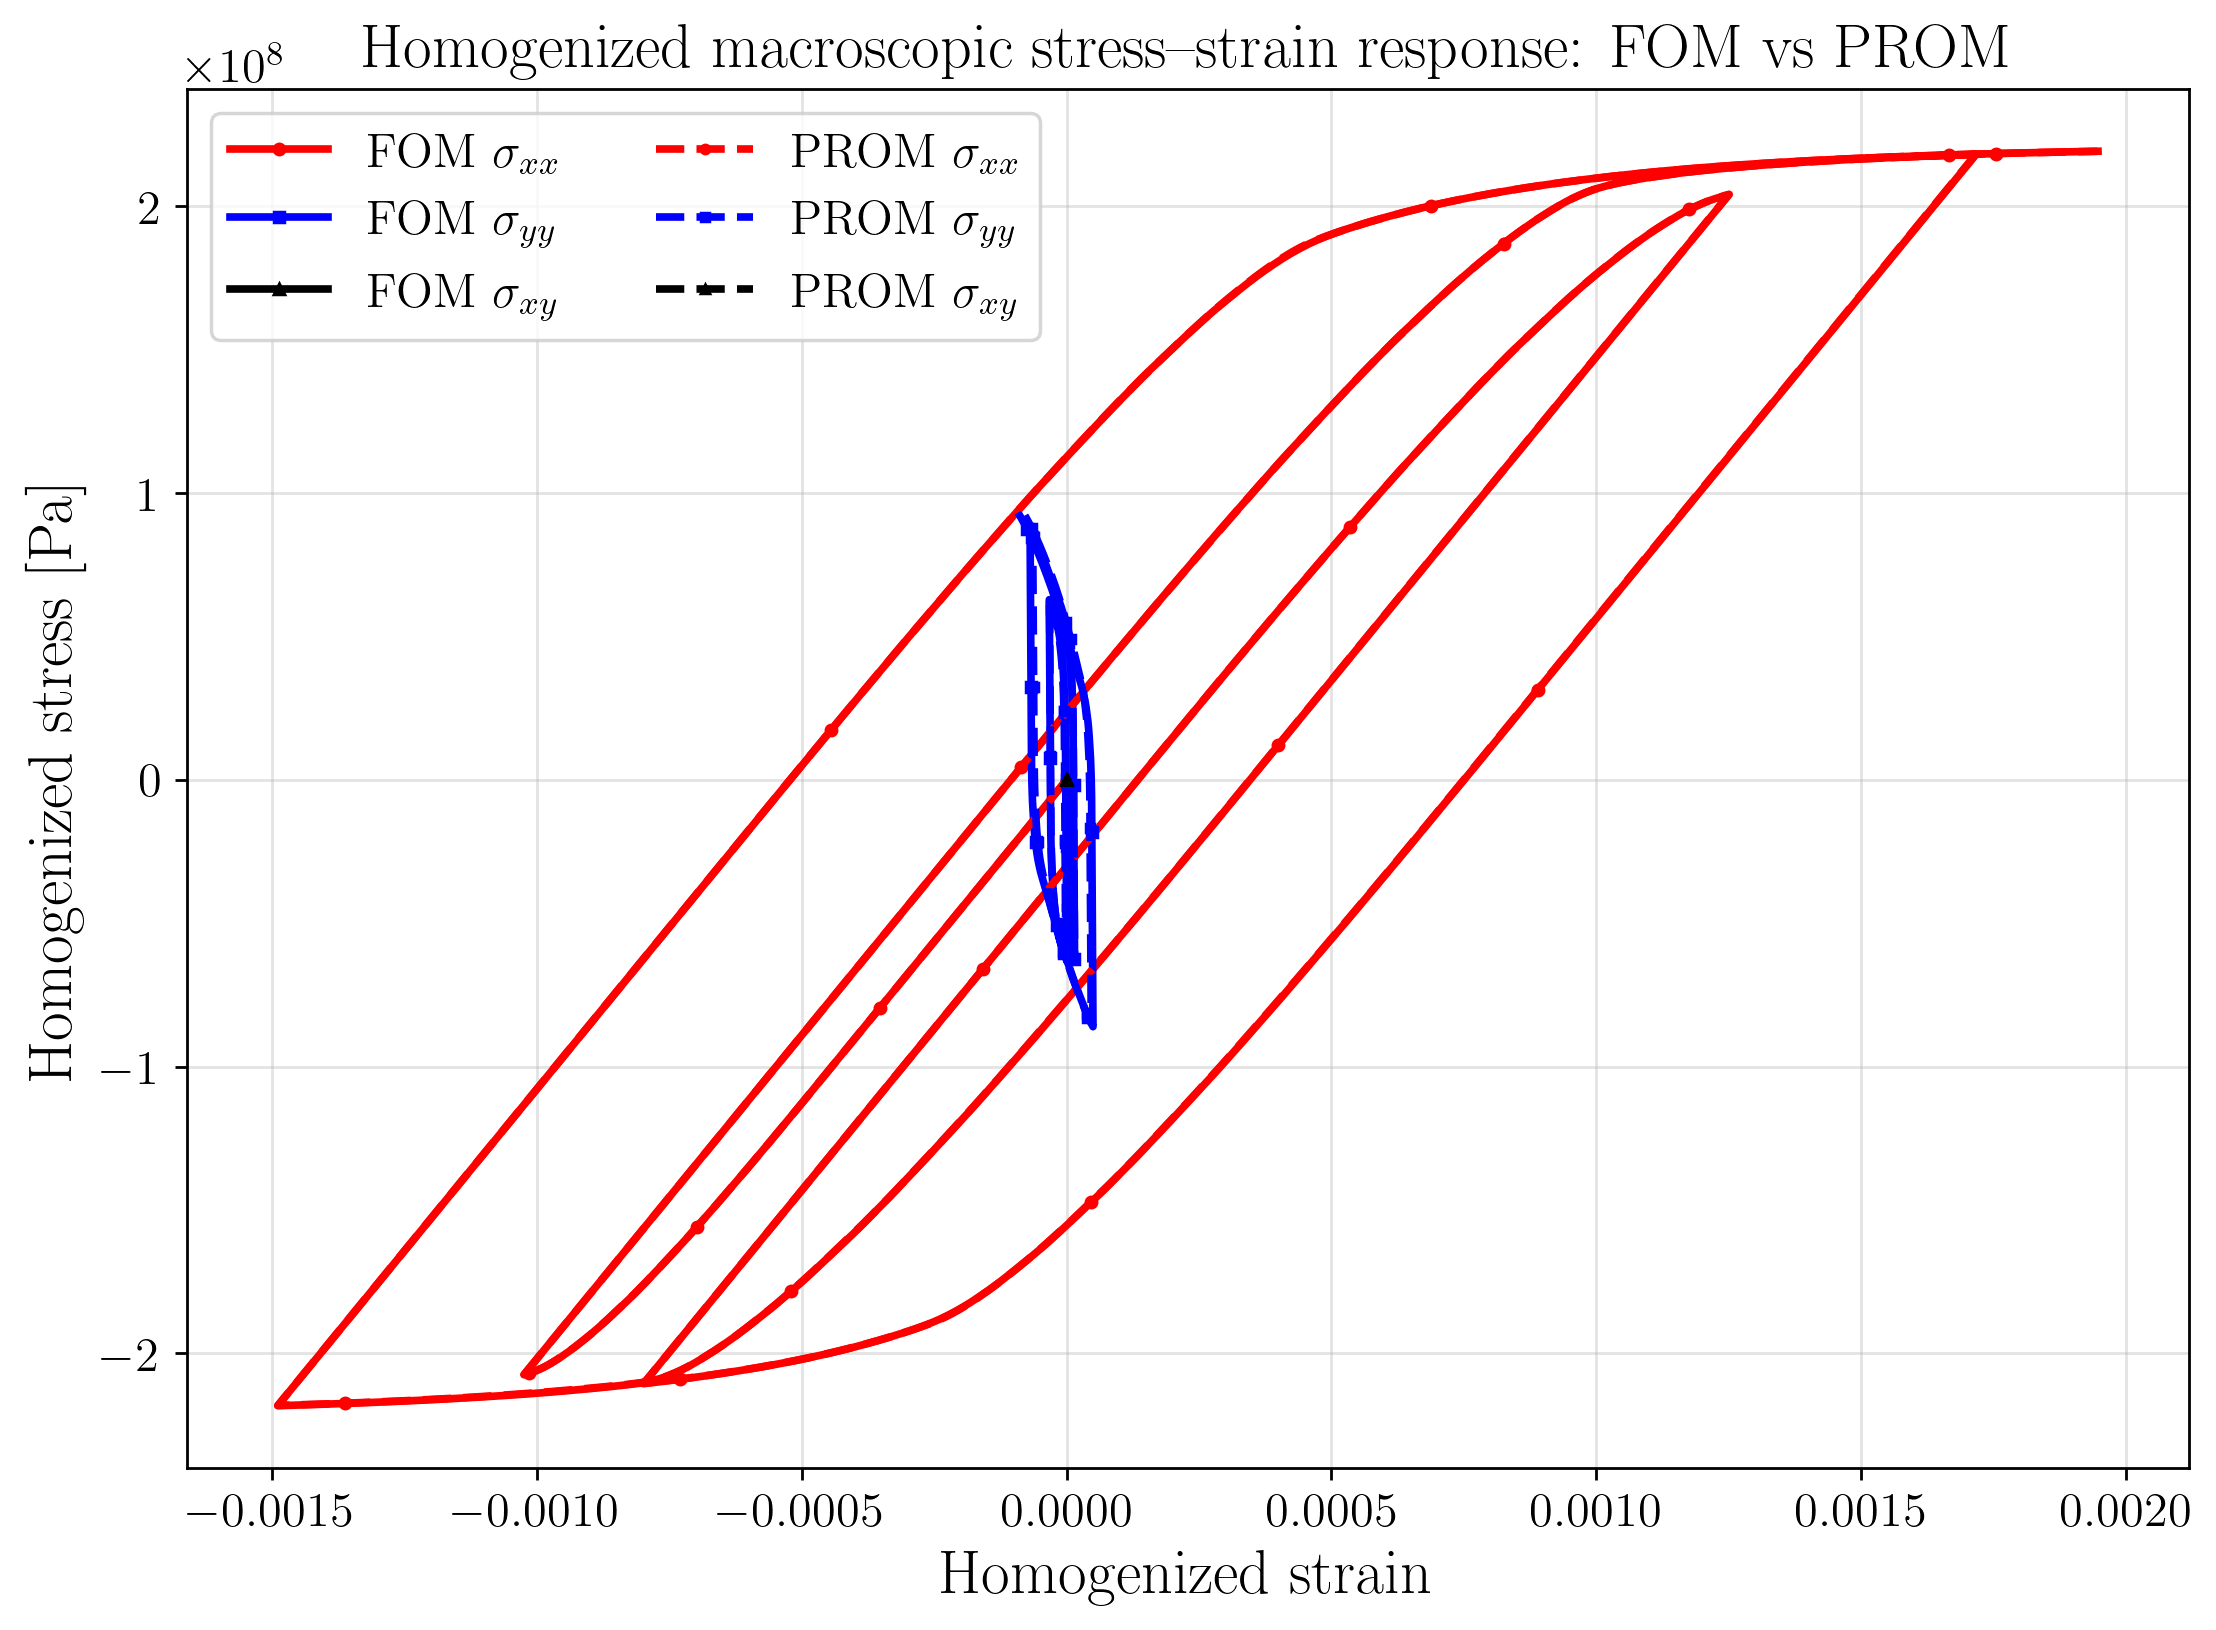
\includegraphics[width=0.78\textwidth]{homogenized_fom_vs_prom.png}
\caption{Comparison between the full-order model and the linear projection-based reduced-order model in terms of homogenized macroscopic stress--strain response along the validation trajectory.}
\label{fig:linear_prom_homogenized_validation}
\end{figure}

The figure shows that the linear PROM reproduces very closely the homogenized response of the RVE throughout the complete loading history, including the segments involving multiple loading reversals. This is a relevant result because the reduced basis was constructed only from two monotonic training trajectories, yet it is already able to generalize successfully to a more complex non-monotonic path.

\subsection{Microscopic Displacement Field Comparison}

In addition to the homogenized quantities, it is important to verify that the reduced model also reproduces the microscopic displacement field with sufficient accuracy. Figure~\ref{fig:linear_prom_field_comparison} shows selected displacement fields obtained from the full-order and reduced-order models at three representative occurrences of the same prescribed macroscopic strain level along the validation trajectory.

\begin{figure}[H]
\centering
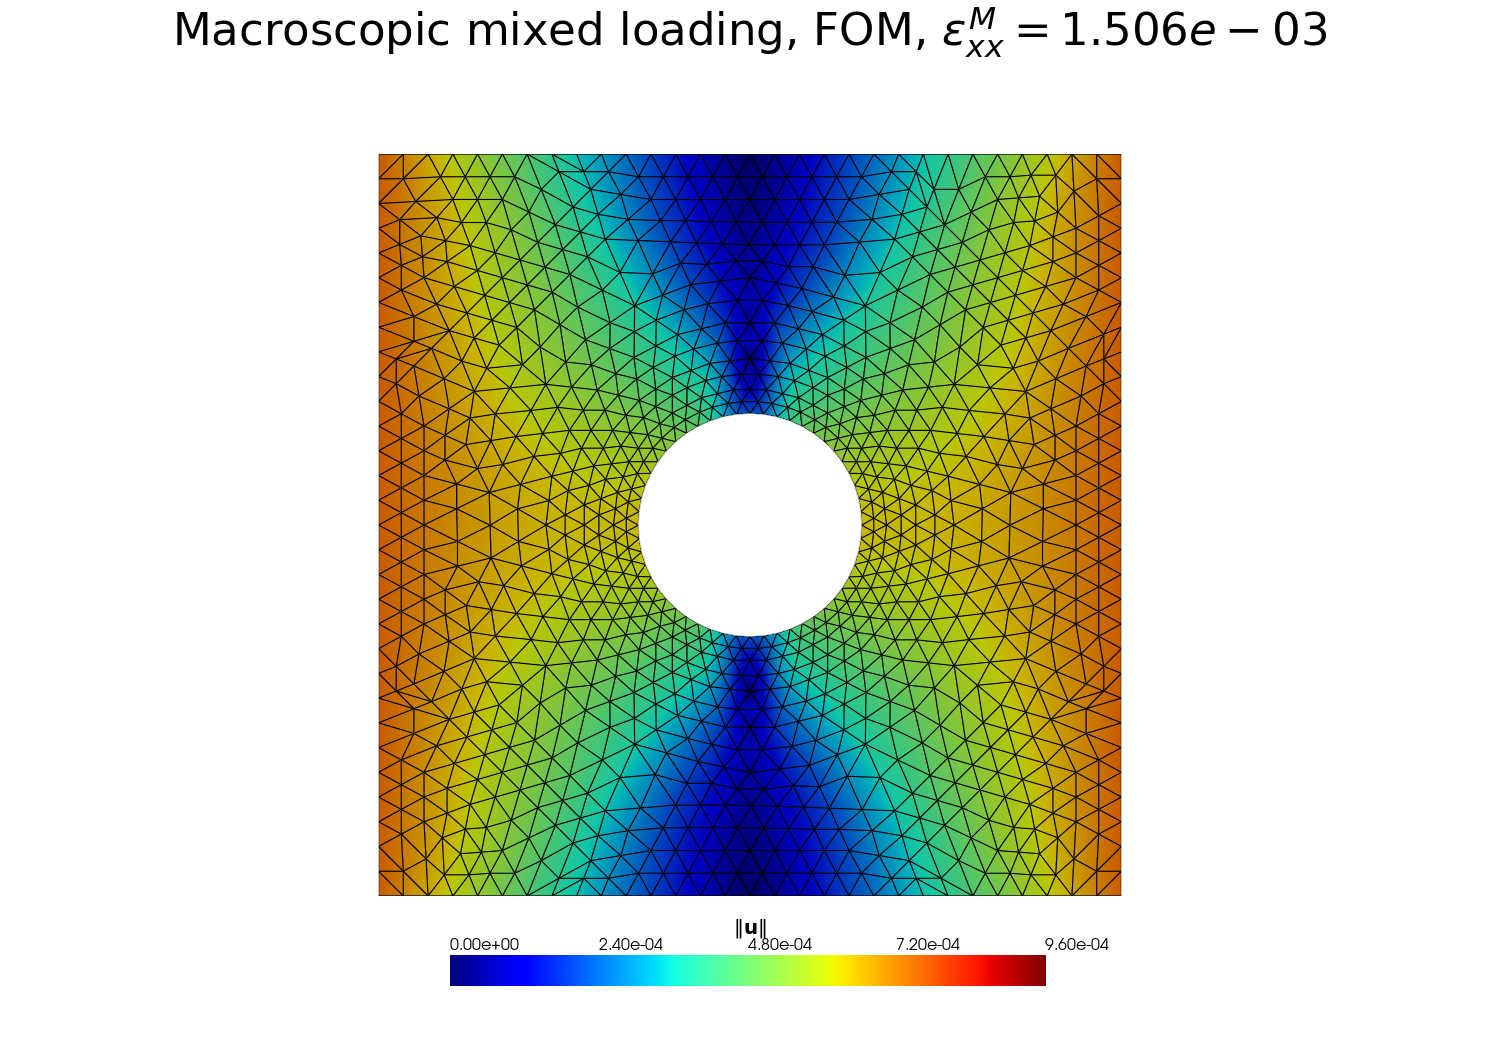
\includegraphics[width=0.32\textwidth]{fom_occurrence_01_step_0364_umag.png}
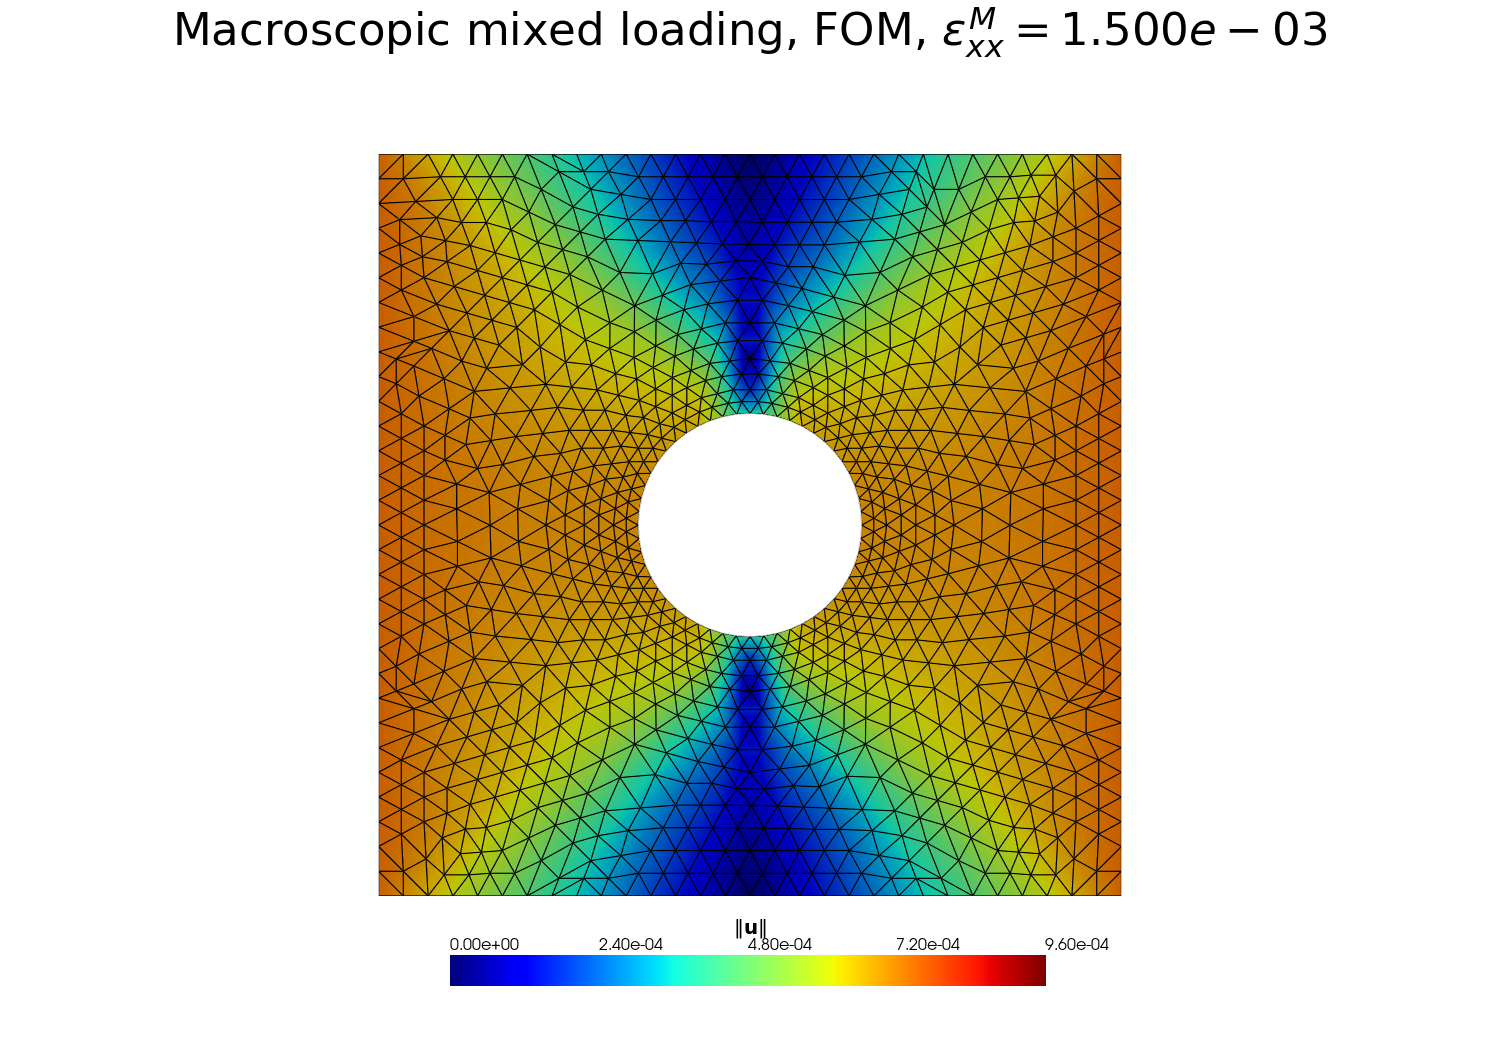
\includegraphics[width=0.32\textwidth]{fom_occurrence_02_step_0440_umag.png}
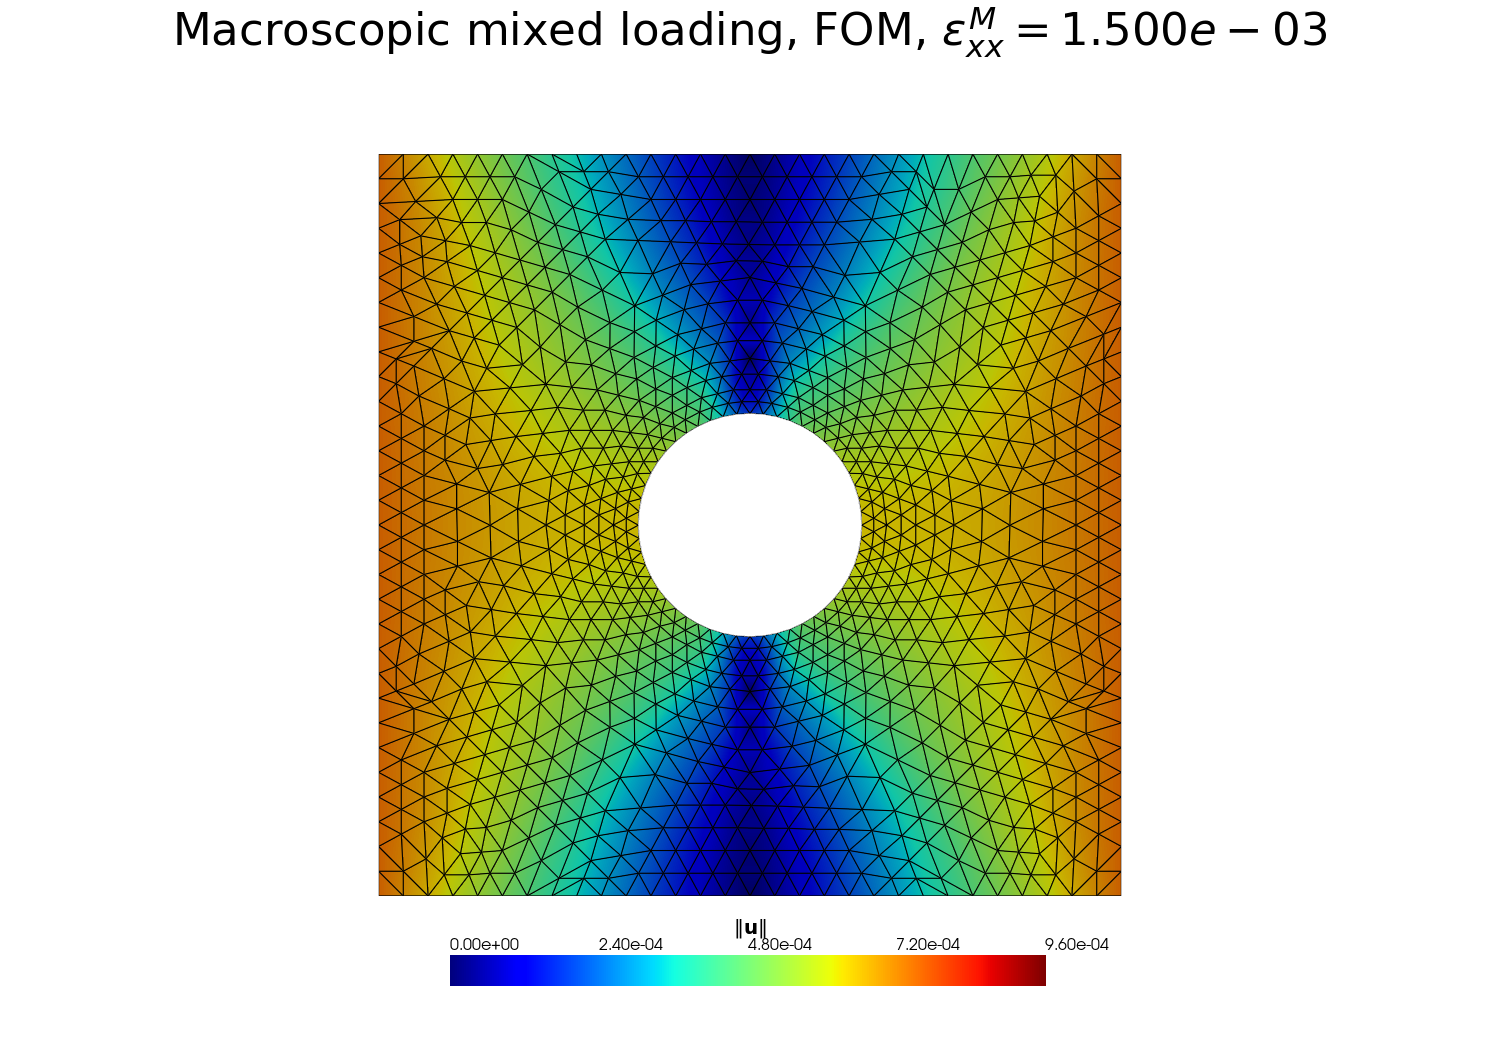
\includegraphics[width=0.32\textwidth]{fom_occurrence_03_step_0800_umag.png}

\vspace{0.5em}

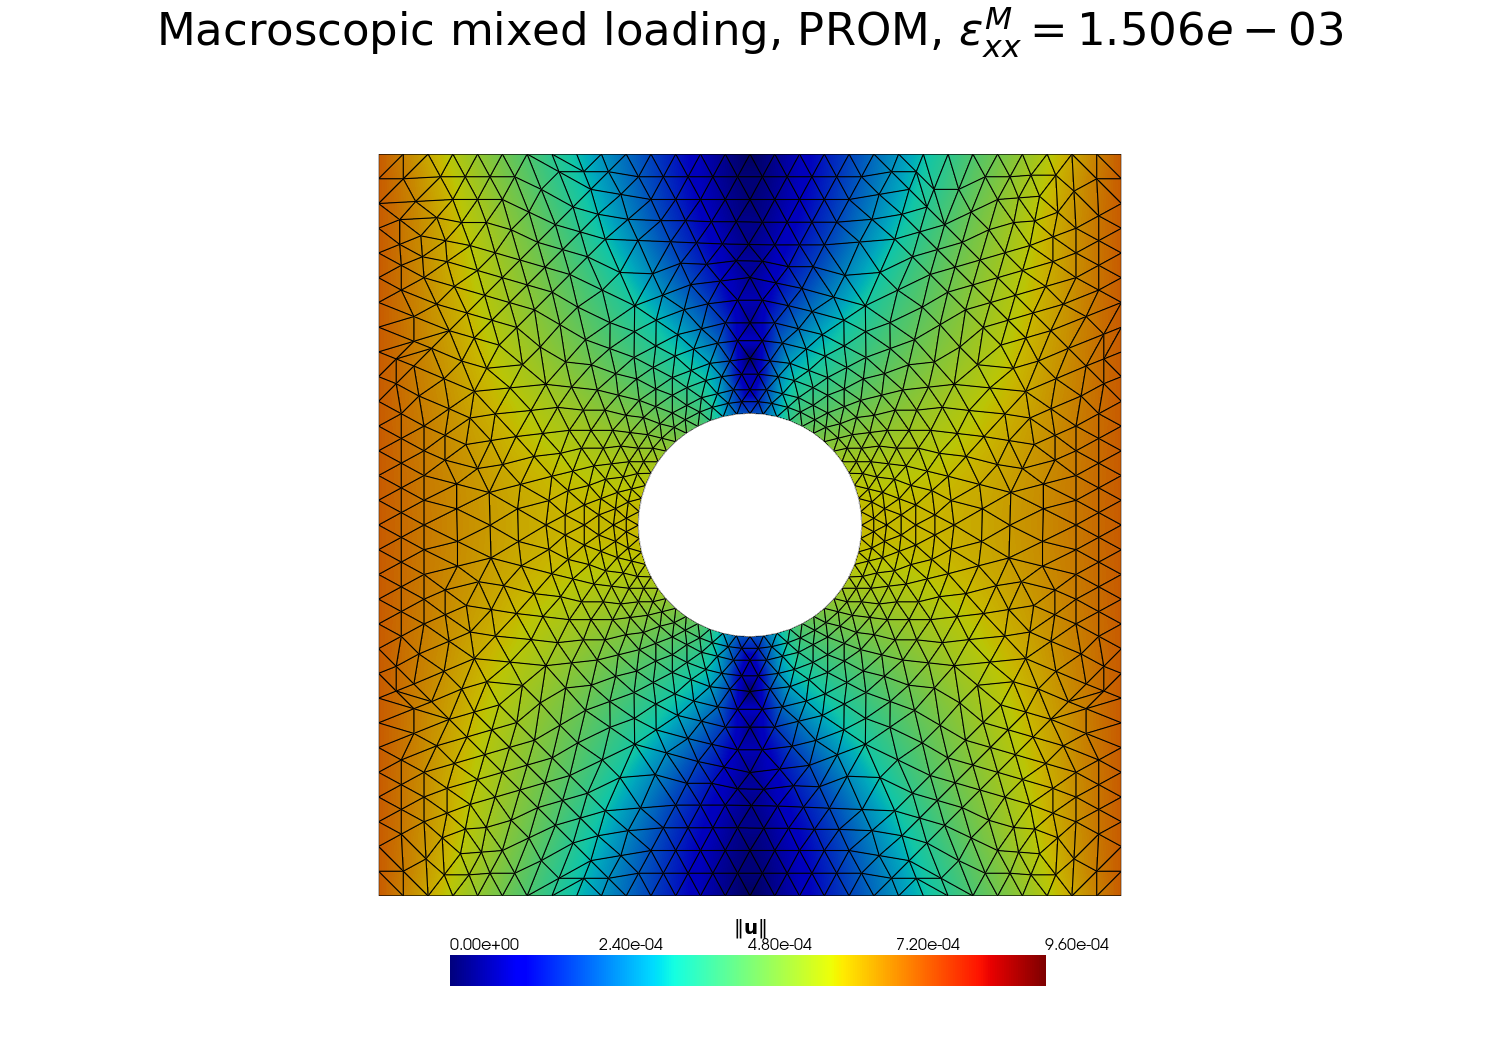
\includegraphics[width=0.32\textwidth]{rom_occurrence_01_step_0364_umag.png}
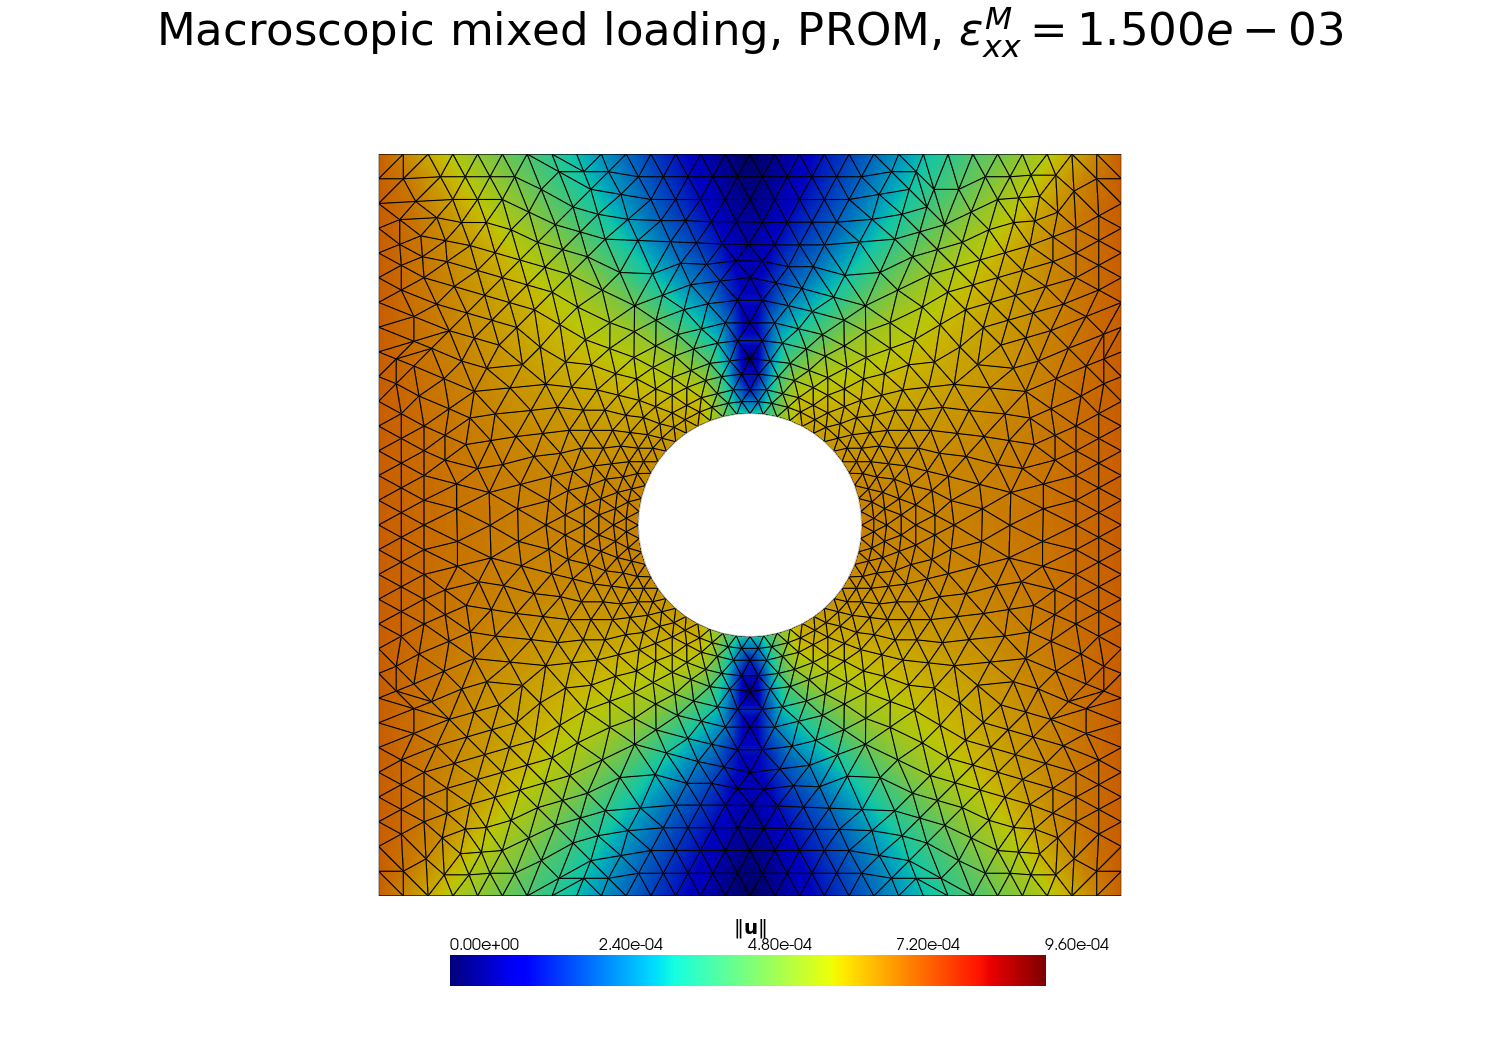
\includegraphics[width=0.32\textwidth]{rom_occurrence_02_step_0440_umag.png}
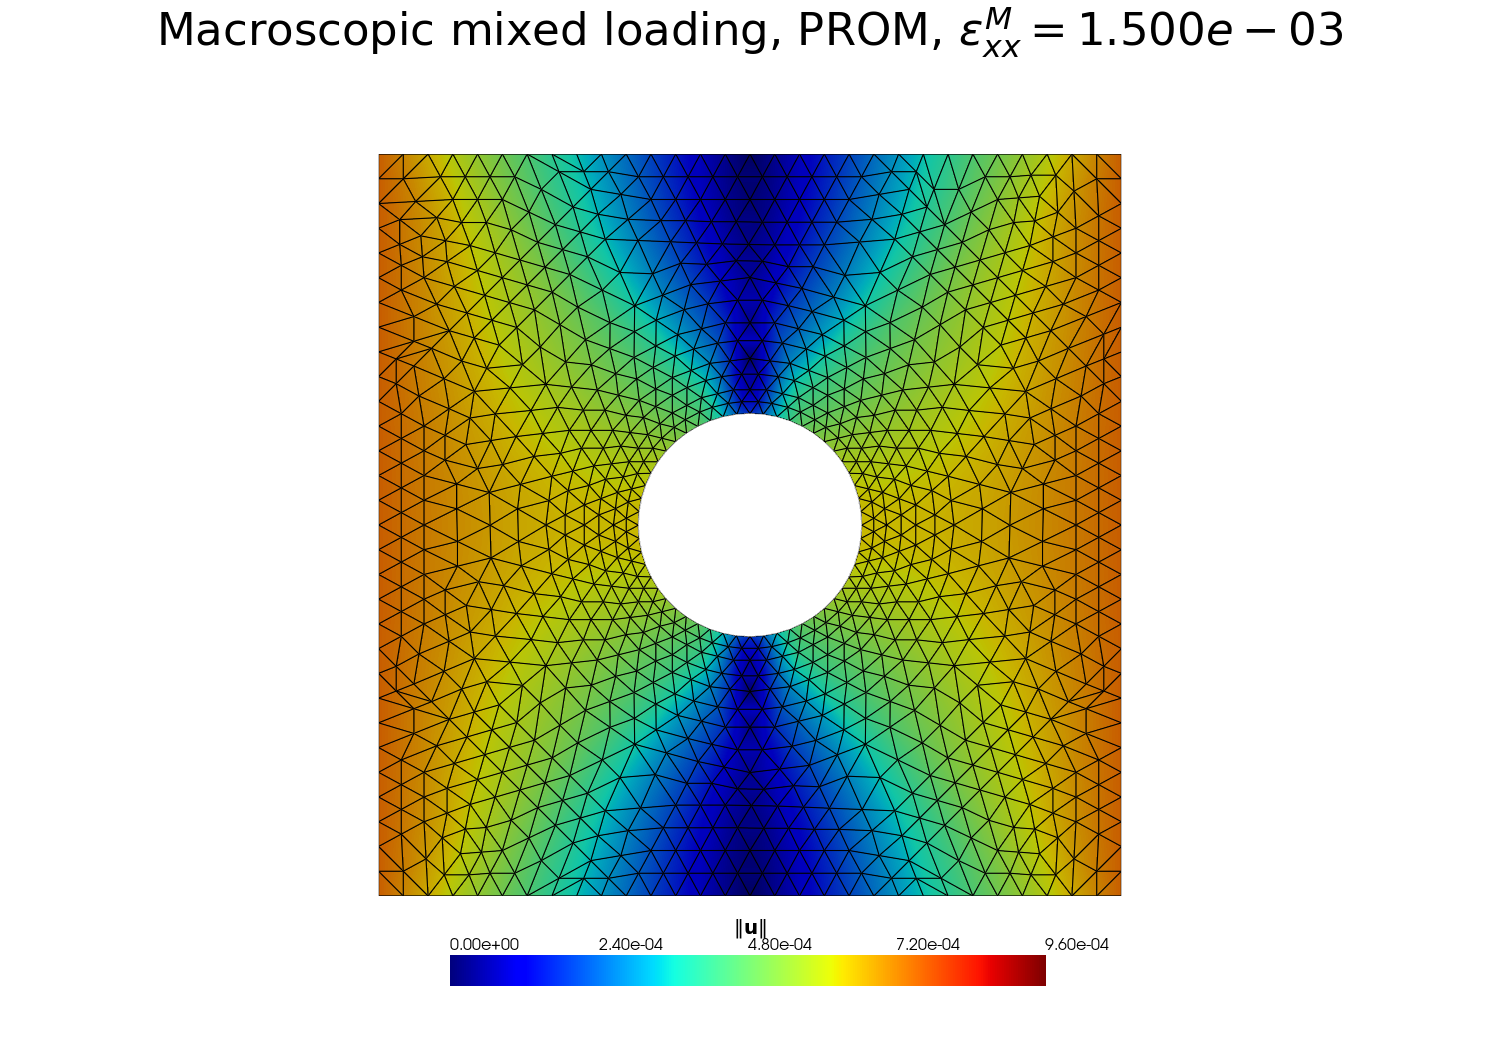
\includegraphics[width=0.32\textwidth]{rom_occurrence_03_step_0800_umag.png}

\caption{Comparison of microscopic displacement fields between the full-order model (top row) and the linear projection-based reduced-order model (bottom row) at three different occurrences of the same prescribed macroscopic strain level along the validation trajectory.}
\label{fig:linear_prom_field_comparison}
\end{figure}

An important observation from these figures is that the three snapshots correspond to nearly identical values of the prescribed macroscopic strain component $\varepsilon_{xx}^{M}$, yet the resulting microscopic displacement fields are not identical. This behavior is expected in an elastoplastic setting, since the internal variables of the constitutive model depend on the loading history experienced by the material. Consequently, two states with the same macroscopic strain may correspond to different microscopic configurations if they are reached through different loading paths.

Despite this path dependence, the linear projection-based reduced-order model is able to reproduce the corresponding displacement fields with very good agreement. The reduced solutions closely match the full-order fields in all three cases, indicating that the reduced basis is sufficiently expressive to capture the variations in the microscopic response associated with different loading histories.

\subsection{Interpretation of the Linear PROM Results}

The previous results show that the linear projection-based reduced-order model is already remarkably effective for this uniaxial RVE problem. In particular, the reduced basis contains only

\begin{equation}
r = 8
\end{equation}

modes, namely one elastic mode and seven plastic modes, and yet it reproduces both the microscopic displacement field and the homogenized macroscopic response with high accuracy.

This compactness is important for two reasons. First, it confirms that the dominant behavior of the present uniaxial problem can be represented in a very low-dimensional linear space. Second, it is also highly beneficial for the future construction of a hyper-reduced model, since the dimension of the reduced basis typically influences the complexity of the hyper-reduction procedure. In general, increasing the number of retained modes tends to increase the number of elements or integration entities required by the hyper-reduced model. Therefore, keeping the basis dimension as small as possible is desirable not only for the PROM itself, but also for the efficiency of the later HPROM.

This observation becomes even more relevant when moving beyond the present setting. Although eight modes are already very few for the current uniaxial two-dimensional case, one expects the number of required linear modes to increase when considering richer loading conditions, such as biaxial paths, or when extending the formulation to three-dimensional RVEs. For this reason, it is natural to seek a reduced representation that remains as compact as possible even as the complexity of the problem increases.

The present results suggest that, for the present problem, the dominant linear structure of the solution can already be captured with an extremely small number of latent variables, namely one elastic contribution together with a very low-dimensional plastic representation. This motivates the next step of the methodology: instead of retaining several plastic modes explicitly in the linear basis, one may attempt to keep only the leading plastic coordinate and reconstruct the remaining plastic content through a nonlinear latent correction. In this way, the goal is not to replace a failing linear PROM, but rather to compress an already successful reduced model even further while preserving its accuracy.

\section{Nonlinear Latent Approximation of the Plastic Reduced Coordinates}

\subsection{Nonlinear Reduced Representation}

The linear projection-based reduced-order model introduced in the previous section approximates the displacement field as

\[
\mathbf{u}
\approx
\mathbf{V}_{\mathrm{el}} \mathbf{q}^{\mathrm{el}}
+
\mathbf{V}_{\mathrm{pl}} \mathbf{q}^{\mathrm{pl}},
\]

where $\mathbf{V}_{\mathrm{el}}$ and $\mathbf{V}_{\mathrm{pl}}$ denote the elastic and plastic basis matrices, and $\mathbf{q}^{\mathrm{el}}$ and $\mathbf{q}^{\mathrm{pl}}$ are the corresponding reduced coordinates.

In the present problem the elastic contribution is essentially one-dimensional, while the plastic component contains several reduced coordinates. Although the linear PROM already provides an accurate approximation of the full-order solution, it is natural to investigate whether the plastic contribution can be further compressed through a nonlinear representation.

To this end we partition the plastic reduced coordinates as

\[
\mathbf{q}^{\mathrm{pl}}
=
\begin{bmatrix}
q^{\mathrm{pl}}_0 \\
\bar{\mathbf{q}}^{\mathrm{pl}}
\end{bmatrix},
\]

where $q^{\mathrm{pl}}_0$ denotes the leading plastic coordinate and $\bar{\mathbf{q}}^{\mathrm{pl}}$ contains the remaining plastic components.

The objective is therefore to reconstruct the remaining plastic coordinates through a nonlinear map

\[
\bar{\mathbf{q}}^{\mathrm{pl}}
\approx
\mathcal{N}(\bar{\mathbf{q}}^{\mathrm{lat}}),
\]

where $\bar{\mathbf{q}}^{\mathrm{lat}}$ denotes a small set of latent variables and $\mathcal{N}(\cdot)$ represents a nonlinear regression operator, for instance implemented through radial basis functions or neural networks.

The resulting nonlinear reduced representation becomes

\[
\mathbf{u}
\approx
\mathbf{V}_{\mathrm{el}} \mathbf{q}^{\mathrm{el}}
+
\mathbf{V}_{\mathrm{pl},0} q^{\mathrm{pl}}_0
+
\bar{\mathbf{V}}_{\mathrm{pl}}
\,\mathcal{N}(\bar{\mathbf{q}}^{\mathrm{lat}}),
\]

where $\mathbf{V}_{\mathrm{pl},0}$ denotes the first plastic mode and $\bar{\mathbf{V}}_{\mathrm{pl}}$ collects the remaining plastic modes.

The central question is therefore how to choose the latent variables entering the nonlinear map. In the present work, this choice is guided by a geometric inspection of the trajectories traced by the plastic reduced coordinates.

\subsection{Testing a Functional Relation Between Plastic Coordinates}

A natural first hypothesis is that the remaining plastic coordinates could be expressed directly as functions of the leading plastic coordinate,

\[
q^{\mathrm{pl}}_i
=
g_i(q^{\mathrm{pl}}_0),
\qquad
i = 1,\dots,r_{\mathrm{pl}}-1.
\]

If such relations existed, the plastic component of the reduced model could in principle be represented using only the coordinate $q^{\mathrm{pl}}_0$.

To test this idea, we examine the evolution of the first two plastic reduced coordinates along several validation trajectories involving loading reversals. Figure~\ref{fig:qpl0_qpl1_trajectories} shows the relation between $q^{\mathrm{pl}}_1$ and $q^{\mathrm{pl}}_0$ along these trajectories.

\begin{figure}[H]
\centering
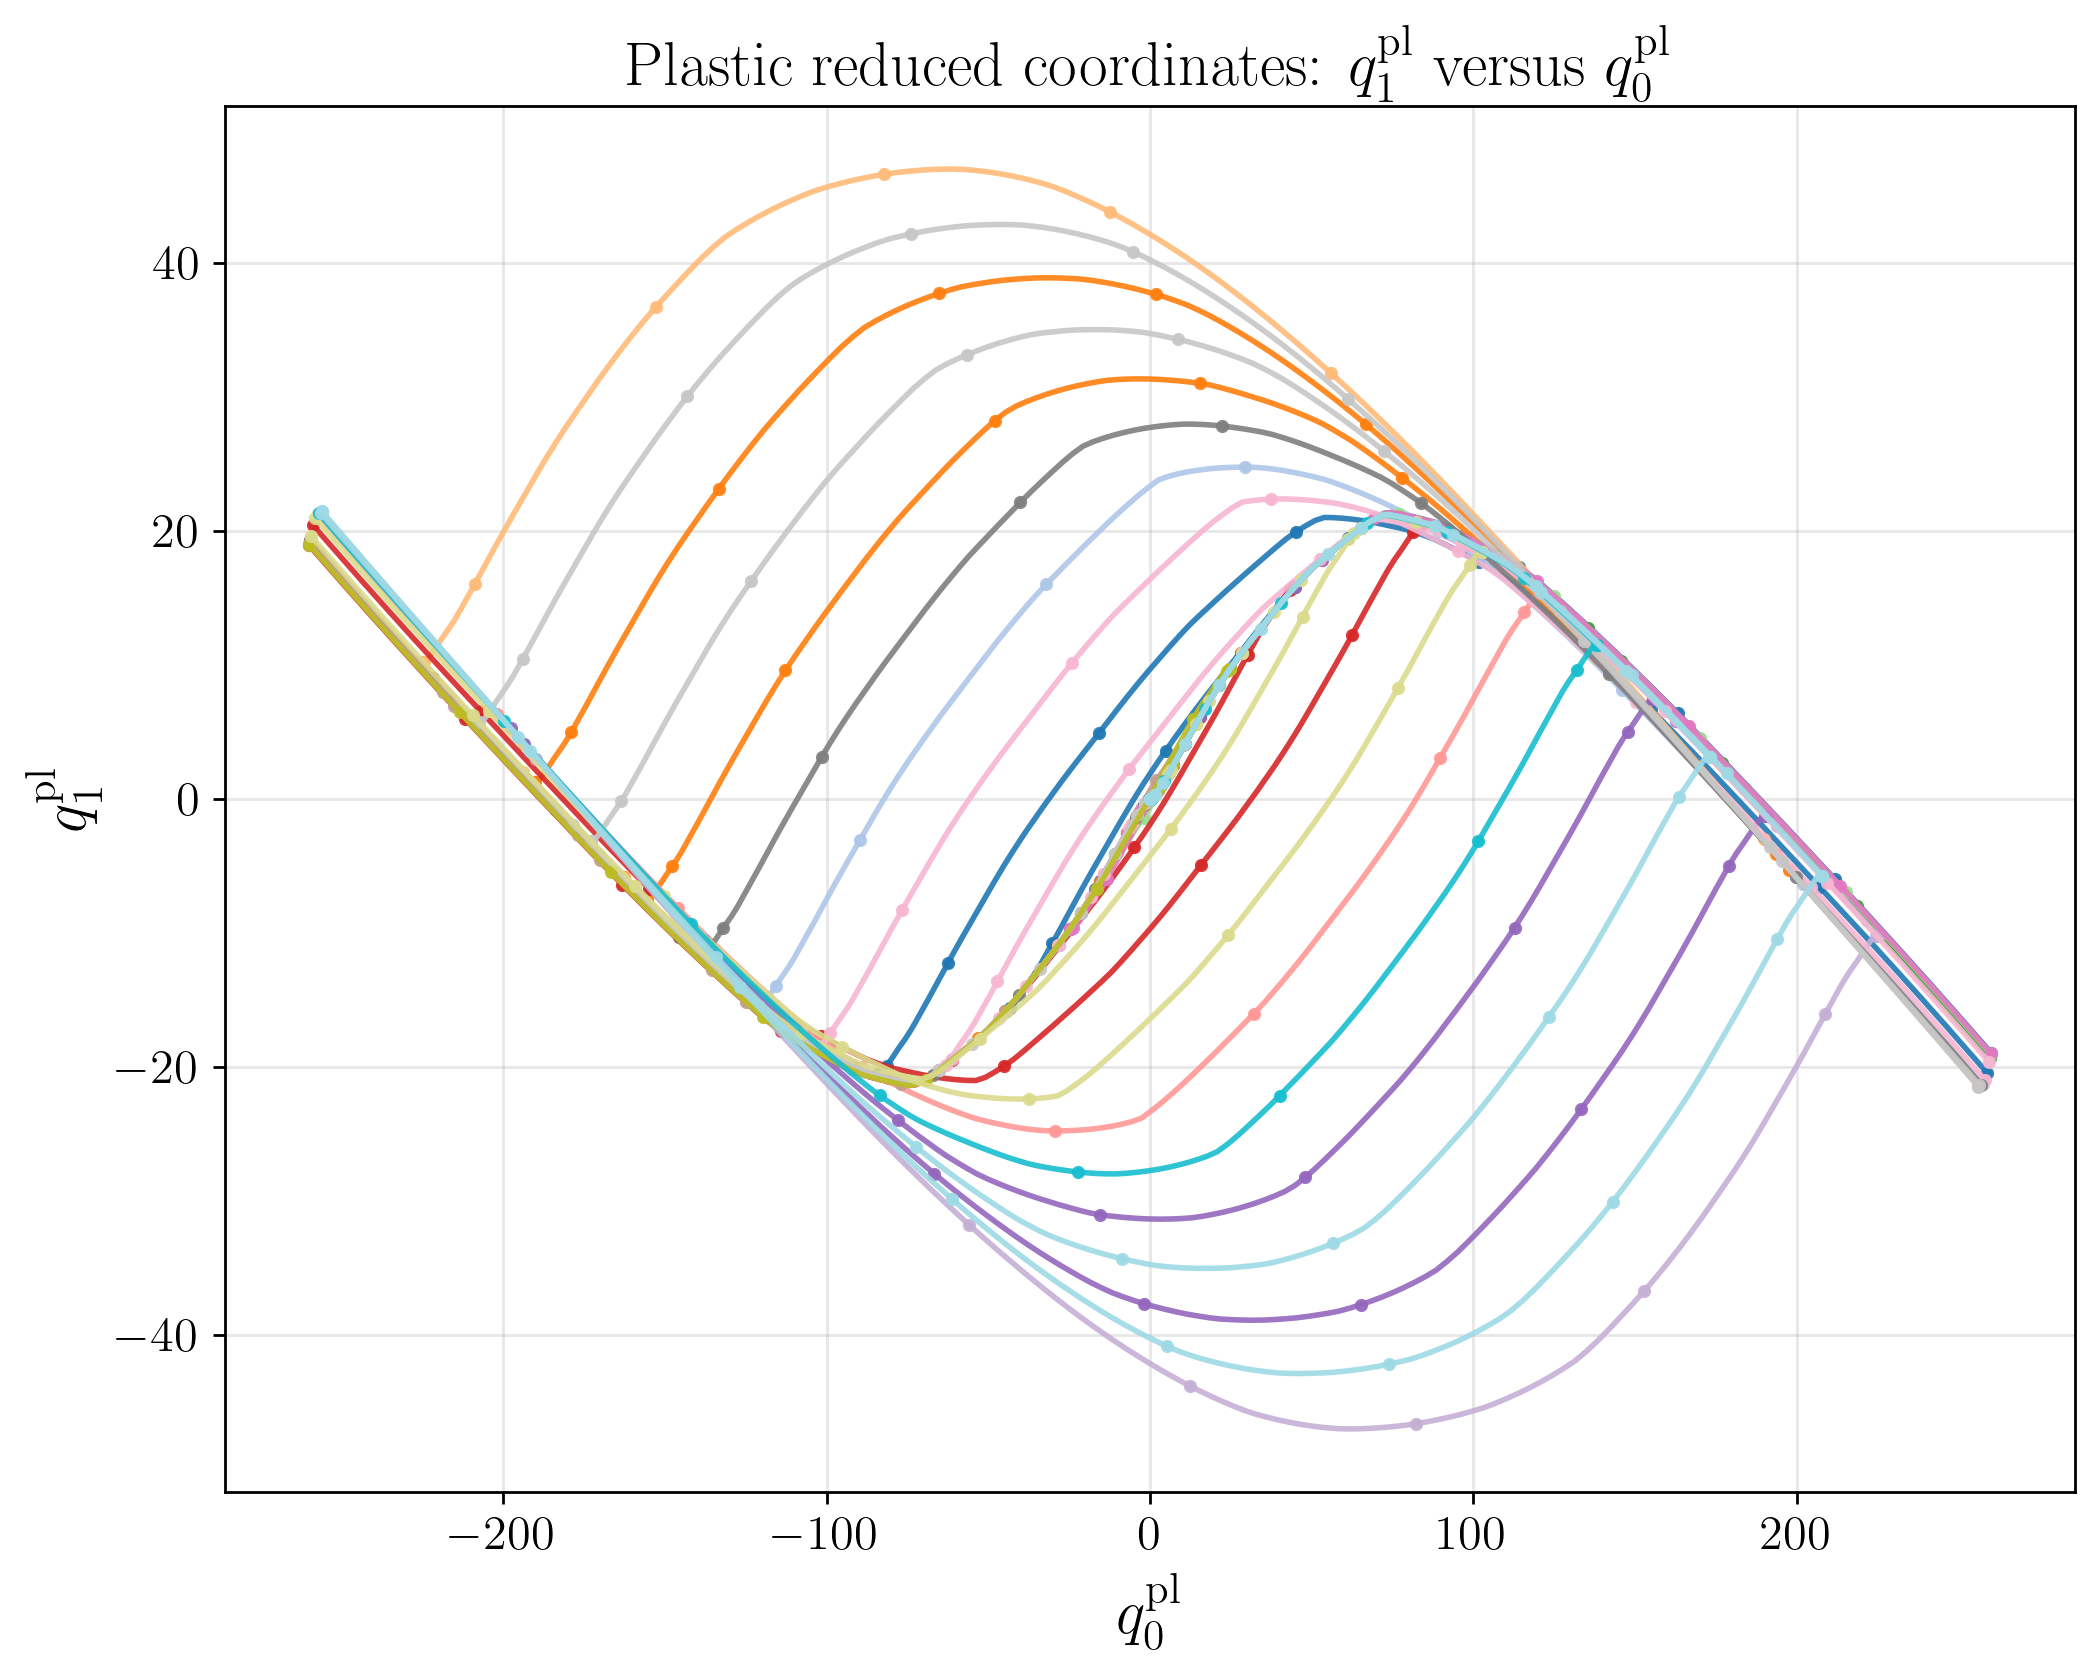
\includegraphics[width=0.75\textwidth]{qpl0_vs_qpl1_rom_only_lines.png}
\caption{Relation between the first two plastic reduced coordinates along several validation trajectories. Different colors correspond to different loading paths.}
\label{fig:qpl0_qpl1_trajectories}
\end{figure}

The figure clearly shows that the relation between the two coordinates is not single-valued. Instead, trajectories corresponding to different loading histories follow different paths in the $(q^{\mathrm{pl}}_0,q^{\mathrm{pl}}_1)$ plane.

Two important conclusions follow from this observation. First, the mapping between the plastic coordinates is path dependent: the same value of $q^{\mathrm{pl}}_0$ may correspond to multiple values of $q^{\mathrm{pl}}_1$ depending on the loading history. Second, the trajectories naturally split into different branches depending on the loading direction.

These observations indicate that a representation of the form $q^{\mathrm{pl}}_i = g_i(q^{\mathrm{pl}}_0)$ is insufficient to describe the plastic evolution of the reduced system.

\subsection{Introduction of an Accumulated Latent Variable \texorpdfstring{$\kappa$}{kappa}}

The previous observations suggest that the plastic state cannot be uniquely characterized by the leading plastic coordinate alone. In classical plasticity theory, path dependence is often described through internal variables measuring accumulated plastic deformation.

Motivated by this idea, we introduce an accumulated latent variable $\kappa$ defined as

\[
\kappa_0 = 0,
\qquad
\kappa_{n+1} =
\kappa_n +
\left|
q^{\mathrm{pl}}_0{}^{(n+1)}
-
q^{\mathrm{pl}}_0{}^{(n)}
\right|.
\]

This variable represents a cumulative measure of plastic evolution along the loading trajectory.

The role of $\kappa$ can be understood by examining the monotonic training trajectories used to construct the reduced basis. Figure~\ref{fig:training_qpl0_kappa} shows the pure tension and pure compression training paths in the $(\kappa,q^{\mathrm{pl}}_0)$ plane.

\begin{figure}[H]
\centering
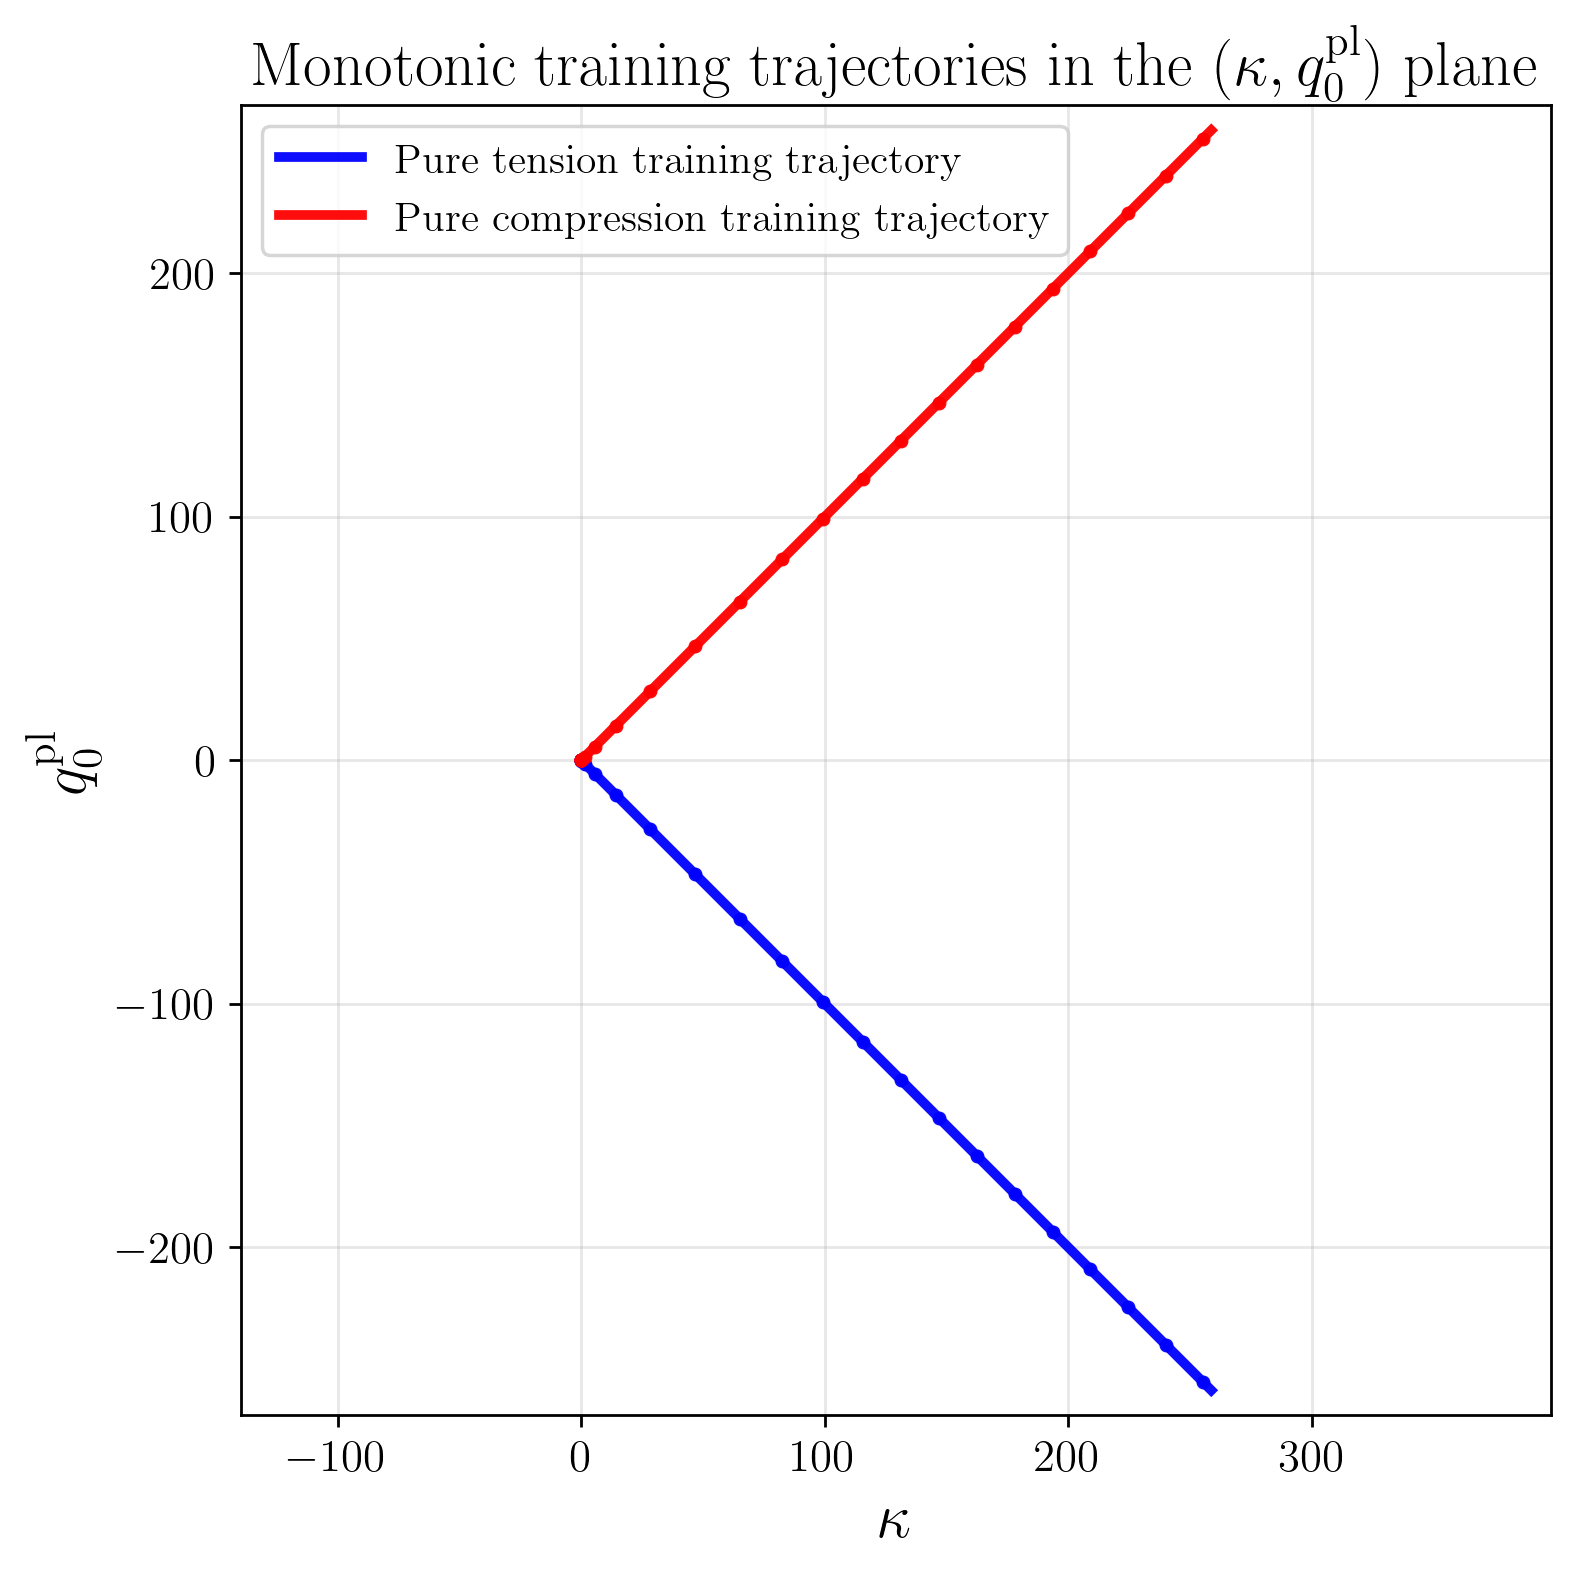
\includegraphics[width=0.60\textwidth]{latent_coordinate_story/training_qpl0_vs_kappa.png}
\caption{Monotonic training trajectories in the $(\kappa,q^{\mathrm{pl}}_0)$ plane.}
\label{fig:training_qpl0_kappa}
\end{figure}

The variable $\kappa$ therefore acts as an accumulated measure of plastic evolution, while the sign of $q^{\mathrm{pl}}_0$ distinguishes the loading direction.

\subsection{Branchwise Latent Structure of One-Reversal Trajectories}

To explore the latent structure beyond monotonic loading, we consider families of trajectories with a single loading reversal. These trajectories start from the origin, evolve first in one loading direction, and then reverse once into the opposite direction.

When represented in the $(\kappa,q^{\mathrm{pl}}_0)$ plane, the resulting trajectories populate a structured region as shown in Figure~\ref{fig:branch_xy_kappa_qpl0}.

\begin{figure}[H]
\centering
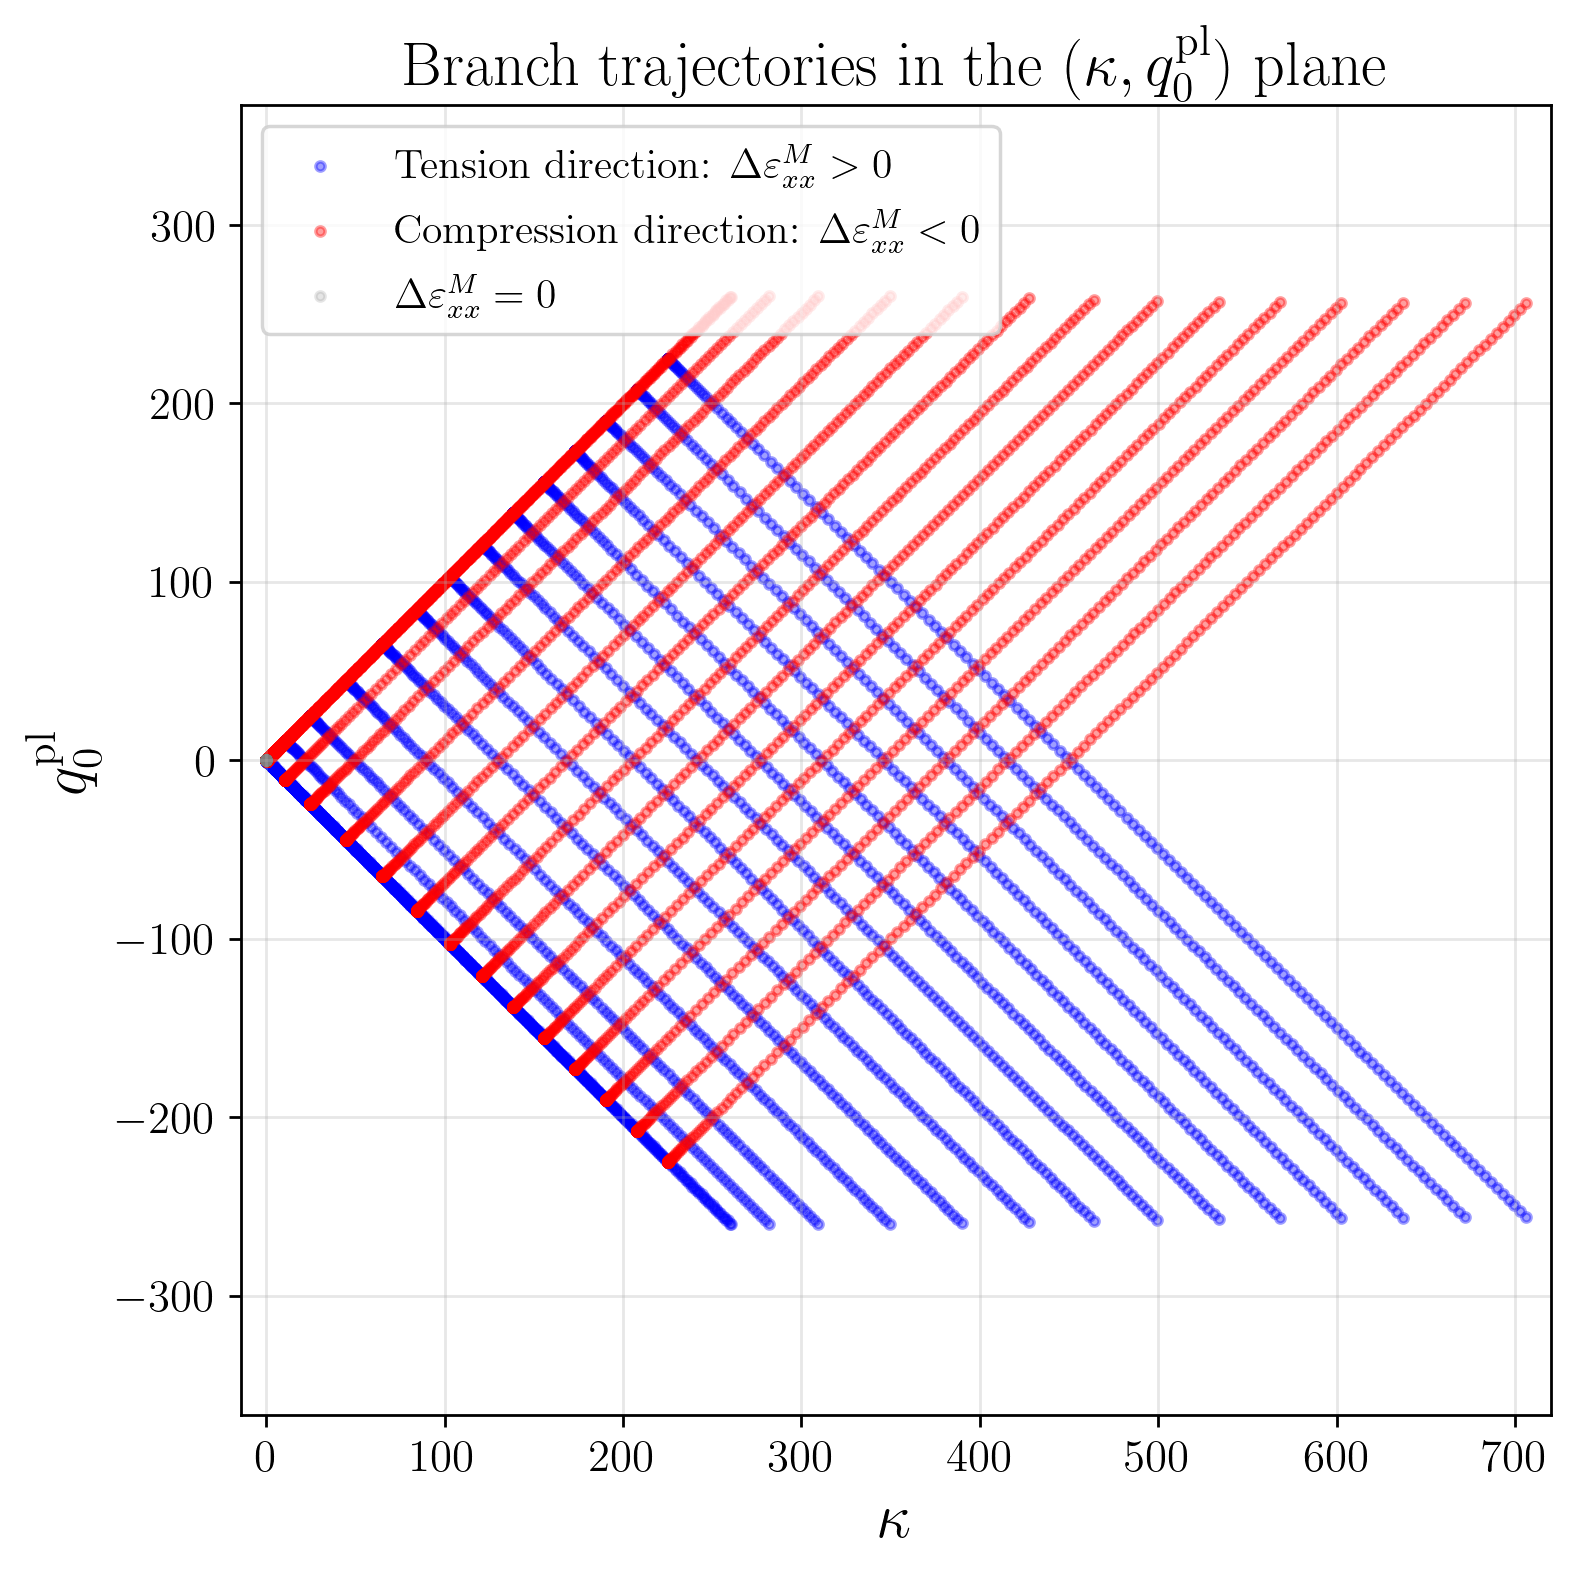
\includegraphics[width=0.70\textwidth]{latent_coordinate_story/branch_only_xy_kappa_vs_qpl0.png}
\caption{One-reversal trajectories in the $(\kappa,q^{\mathrm{pl}}_0)$ plane.}
\label{fig:branch_xy_kappa_qpl0}
\end{figure}

The trajectories are colored according to the sign of the loading increment $\Delta\varepsilon_{xx}^{M}$. Blue points correspond to positive increments, while red points correspond to negative increments.

The resulting point cloud exhibits a clear branchwise structure. Points corresponding to positive and negative loading increments populate two distinct regions of the latent space.

A clearer picture emerges when the trajectories are visualized in the three-dimensional space $(\kappa,q^{\mathrm{pl}}_0,q^{\mathrm{pl}}_1)$, as shown in Figure~\ref{fig:branch_3d_views}.

\begin{figure}[H]
\centering
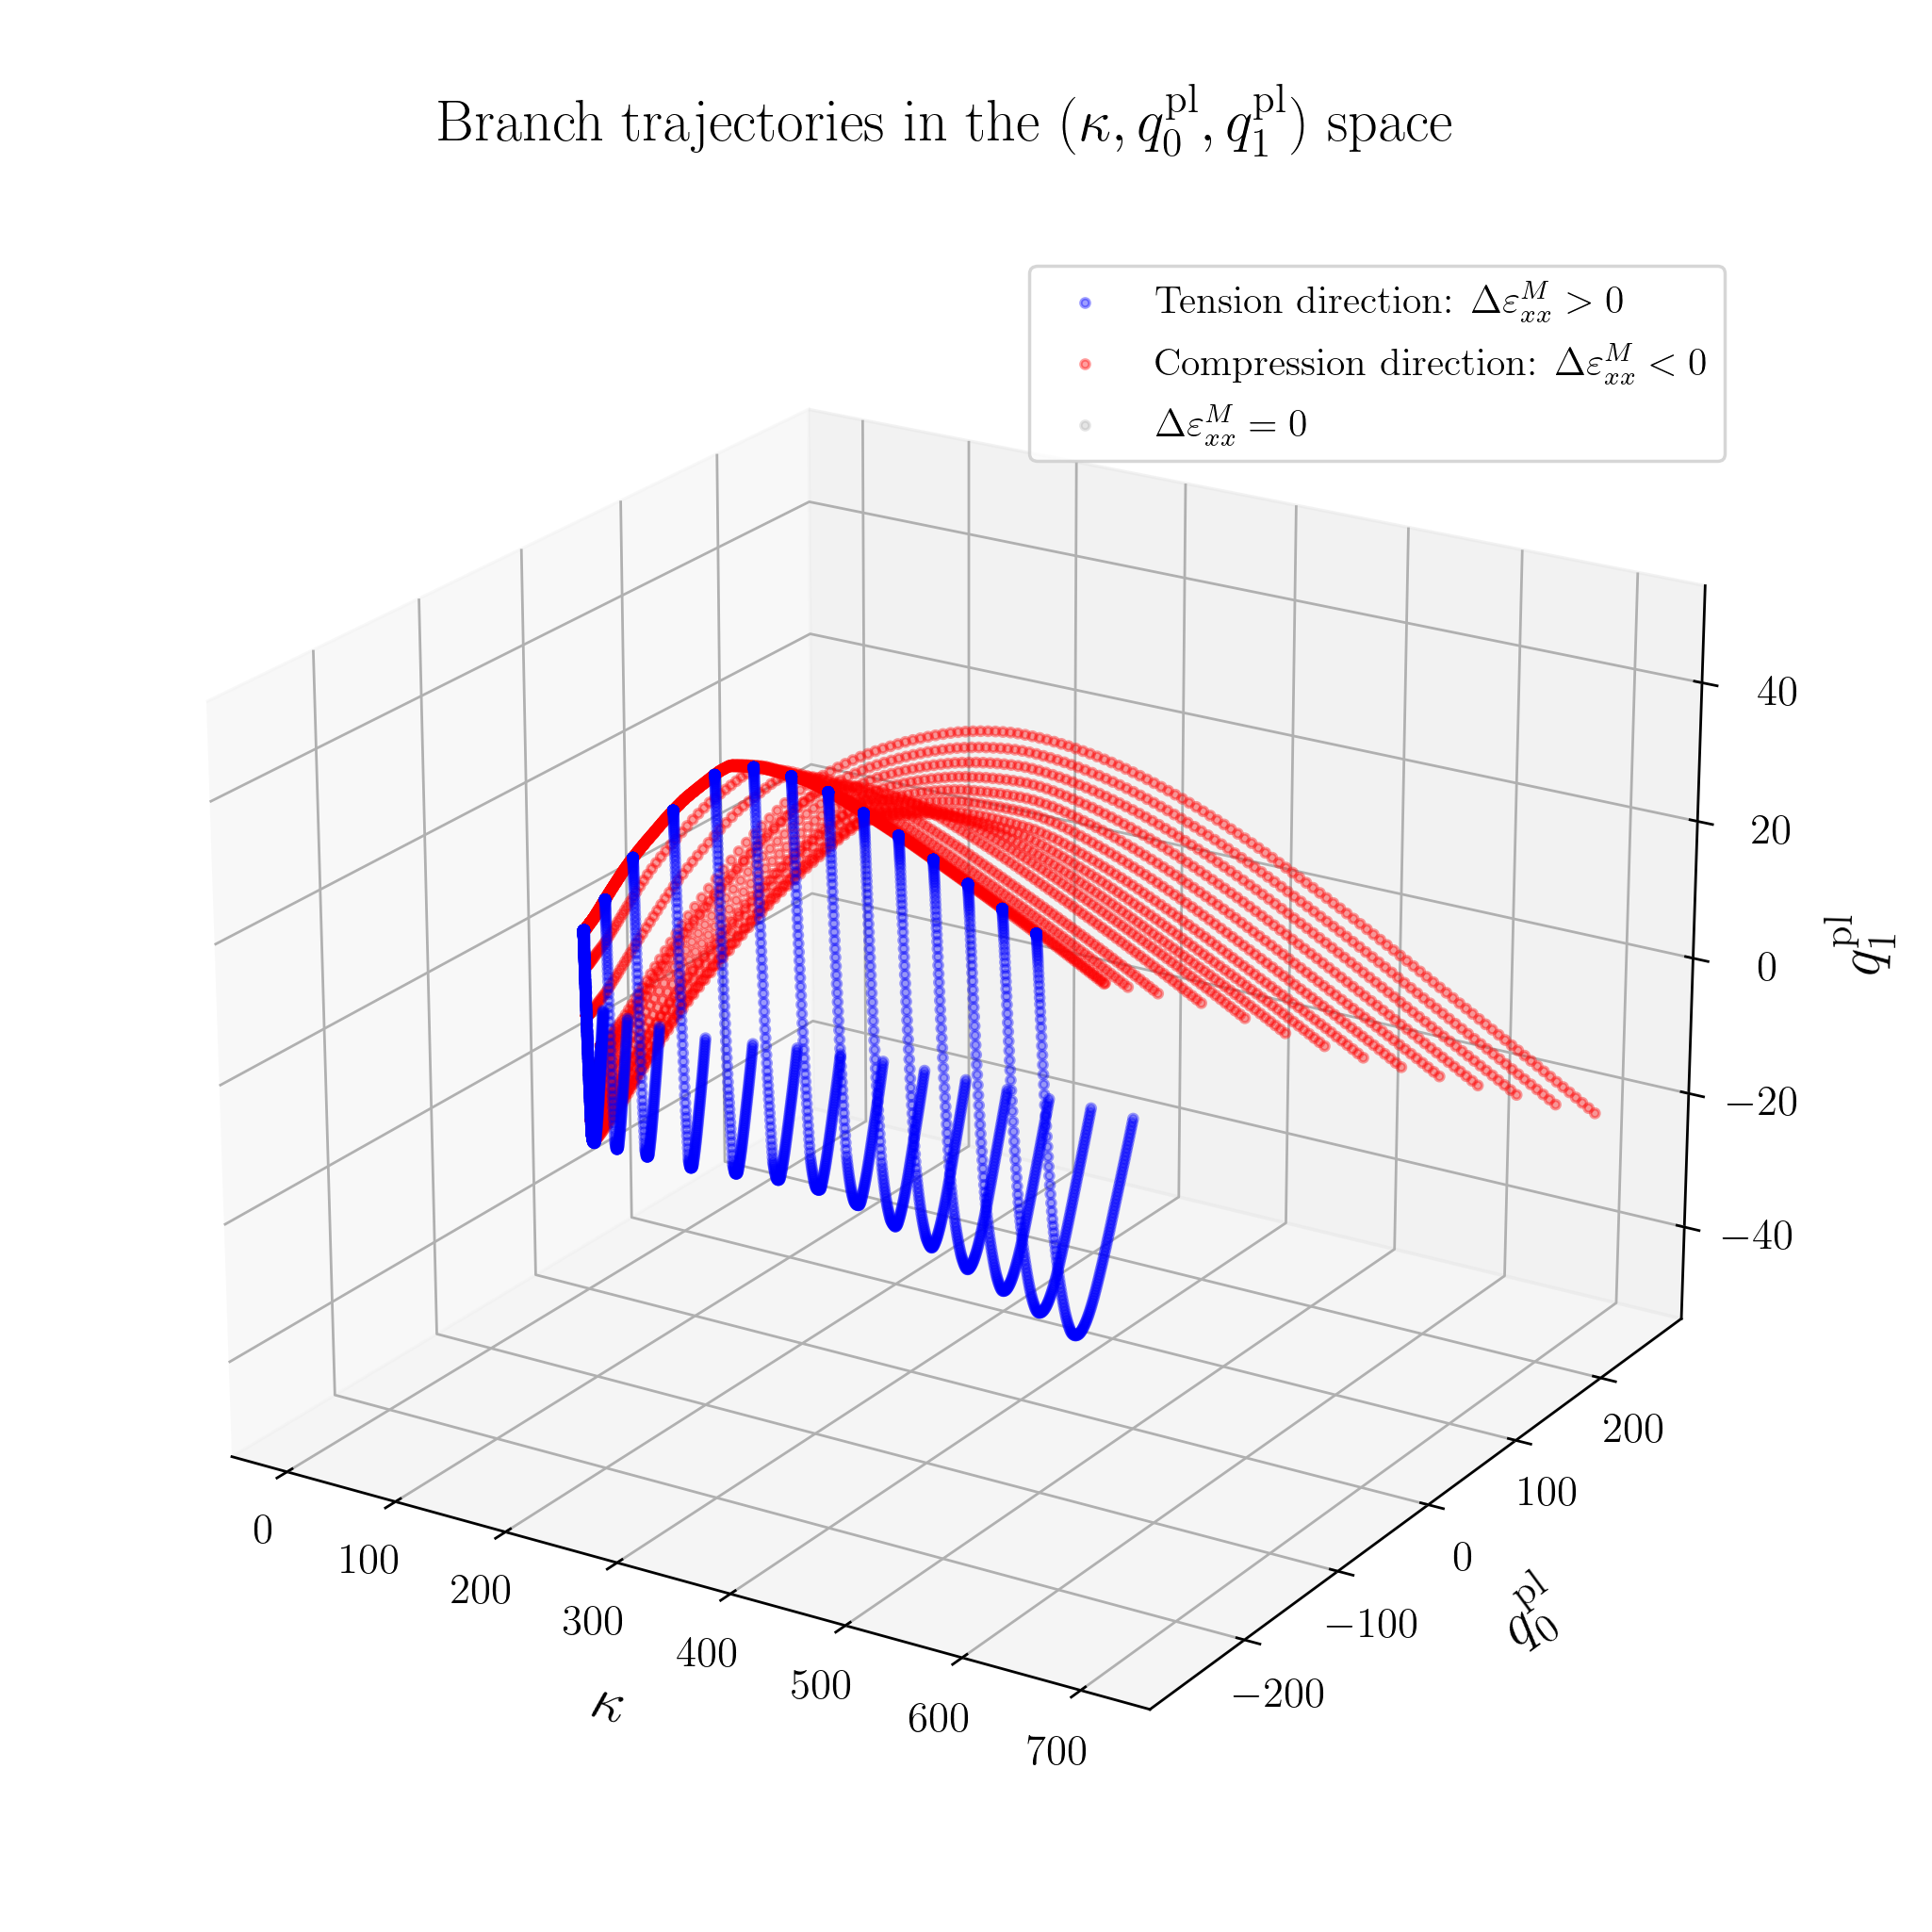
\includegraphics[width=0.32\textwidth]{latent_coordinate_story/branch_only_3d_kappa_qpl0_qpl1_view1.png}
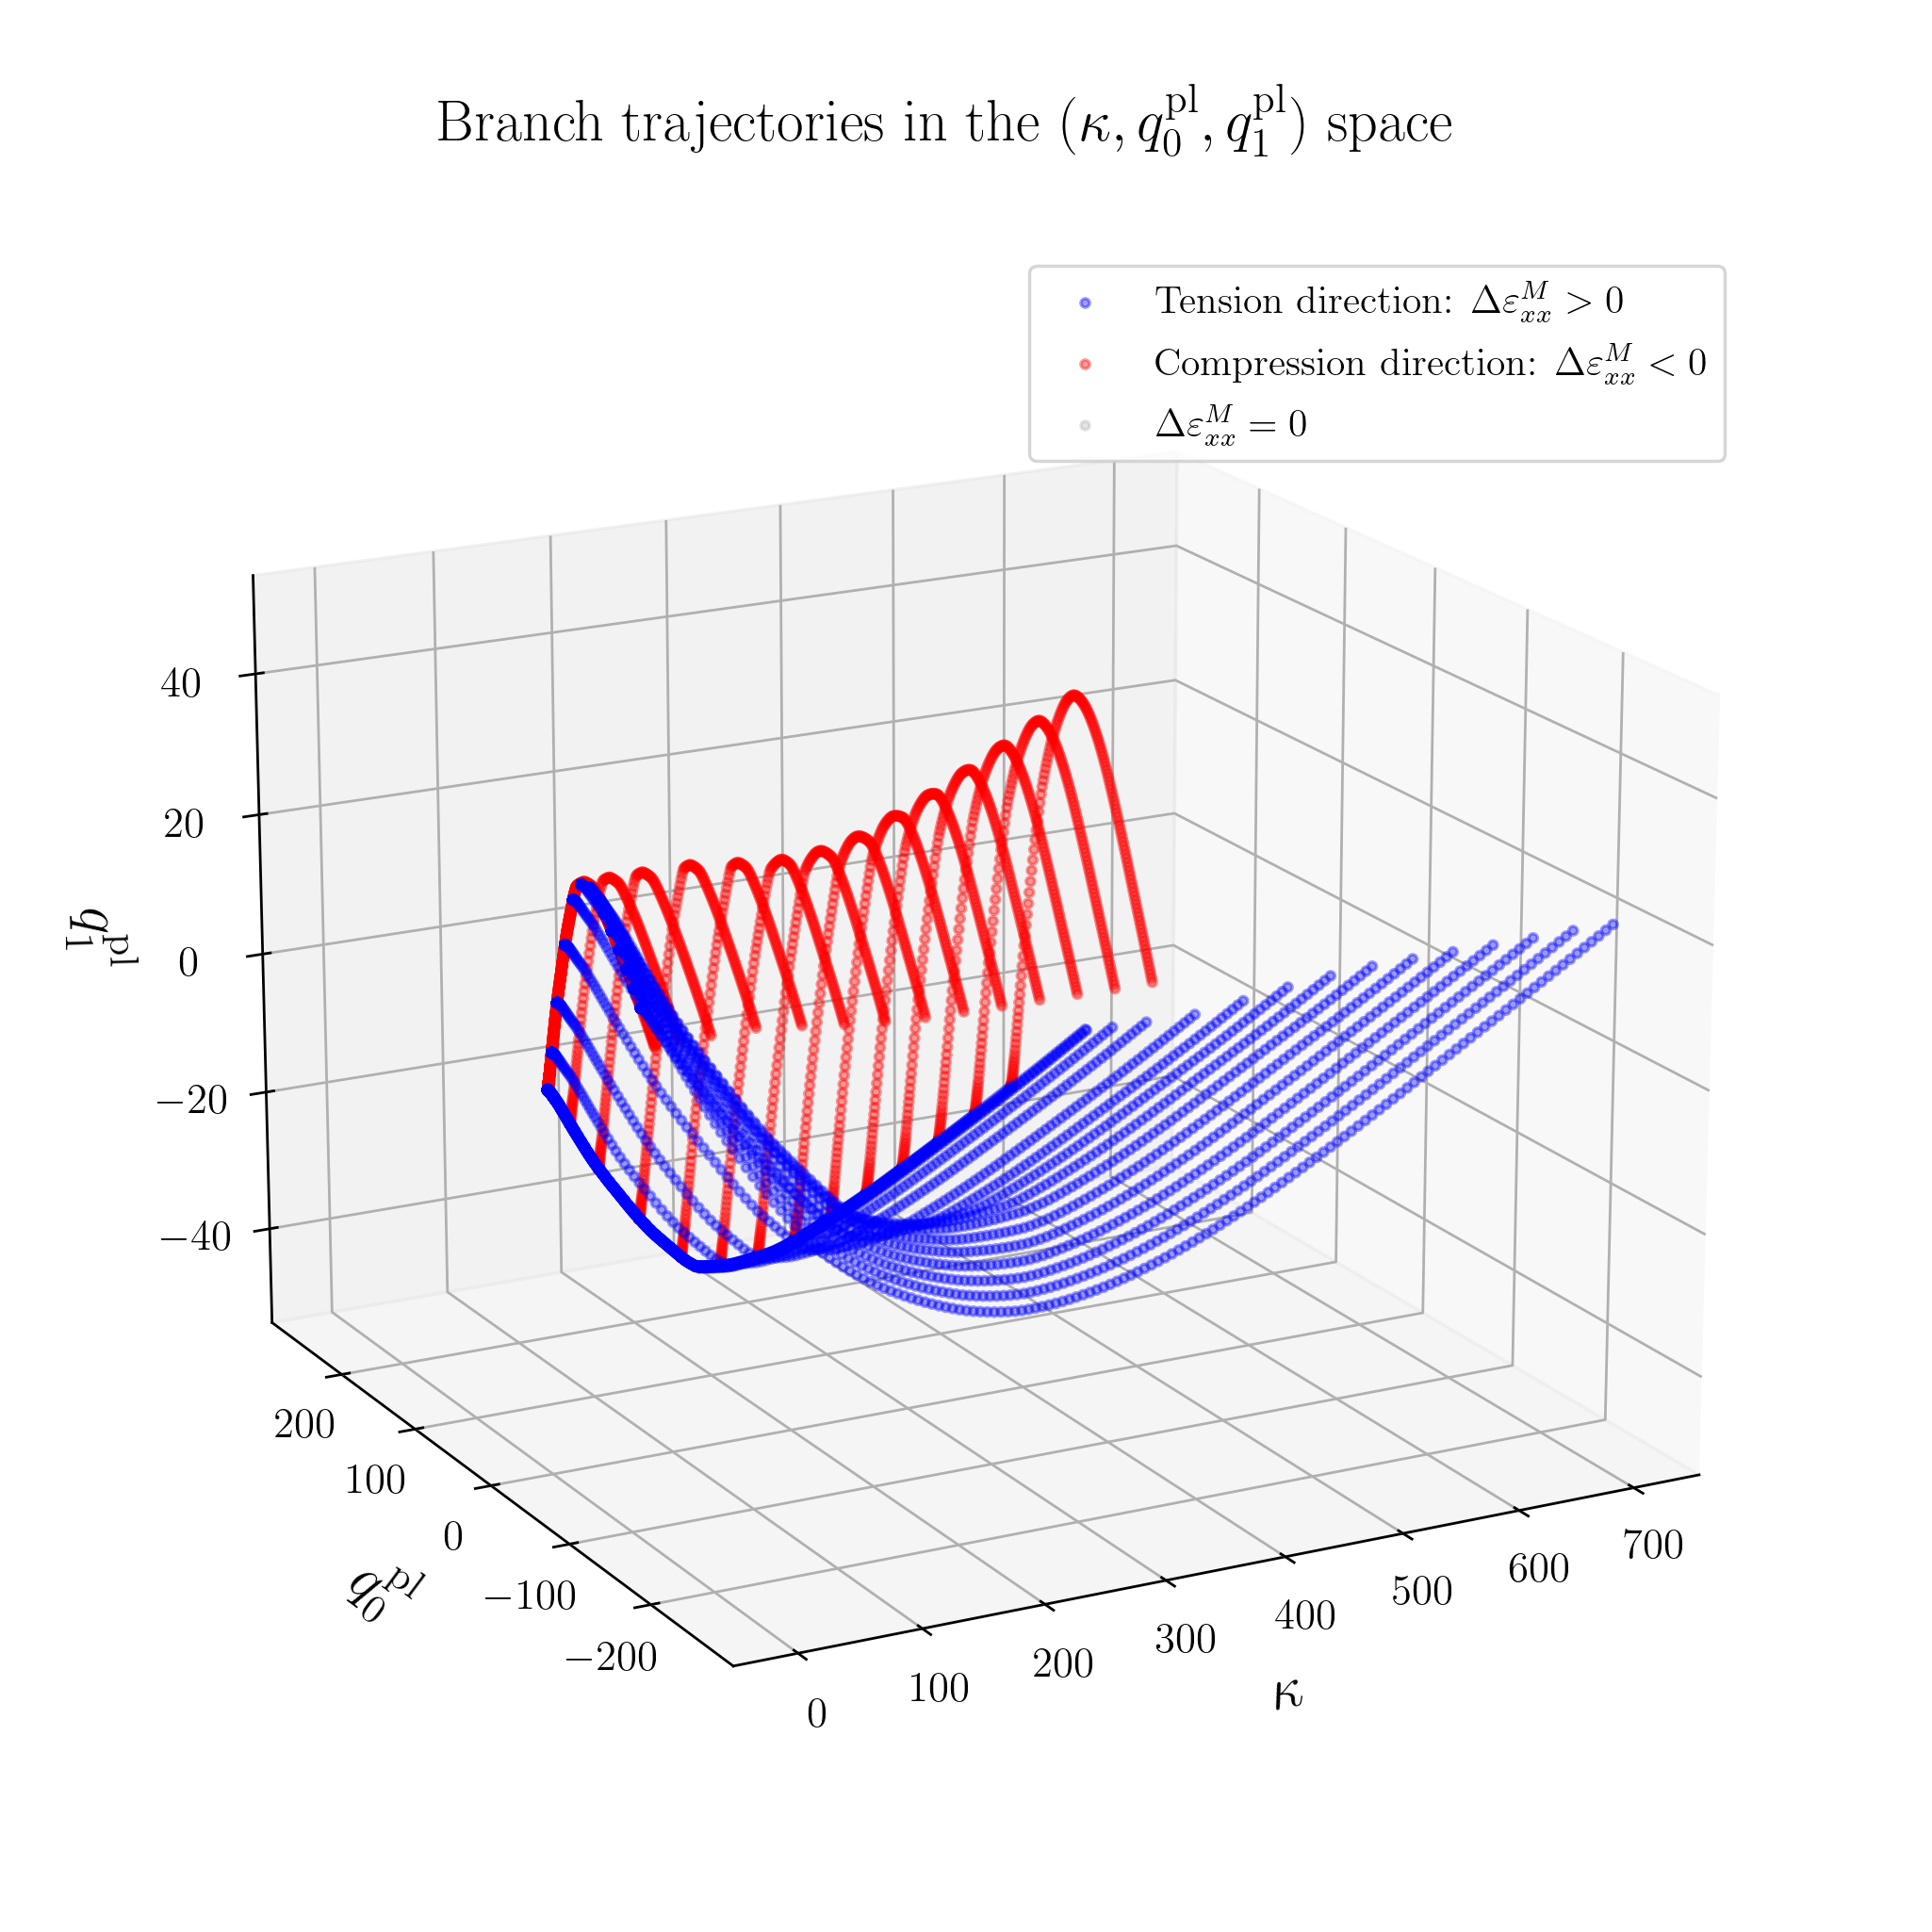
\includegraphics[width=0.32\textwidth]{latent_coordinate_story/branch_only_3d_kappa_qpl0_qpl1_view2.png}
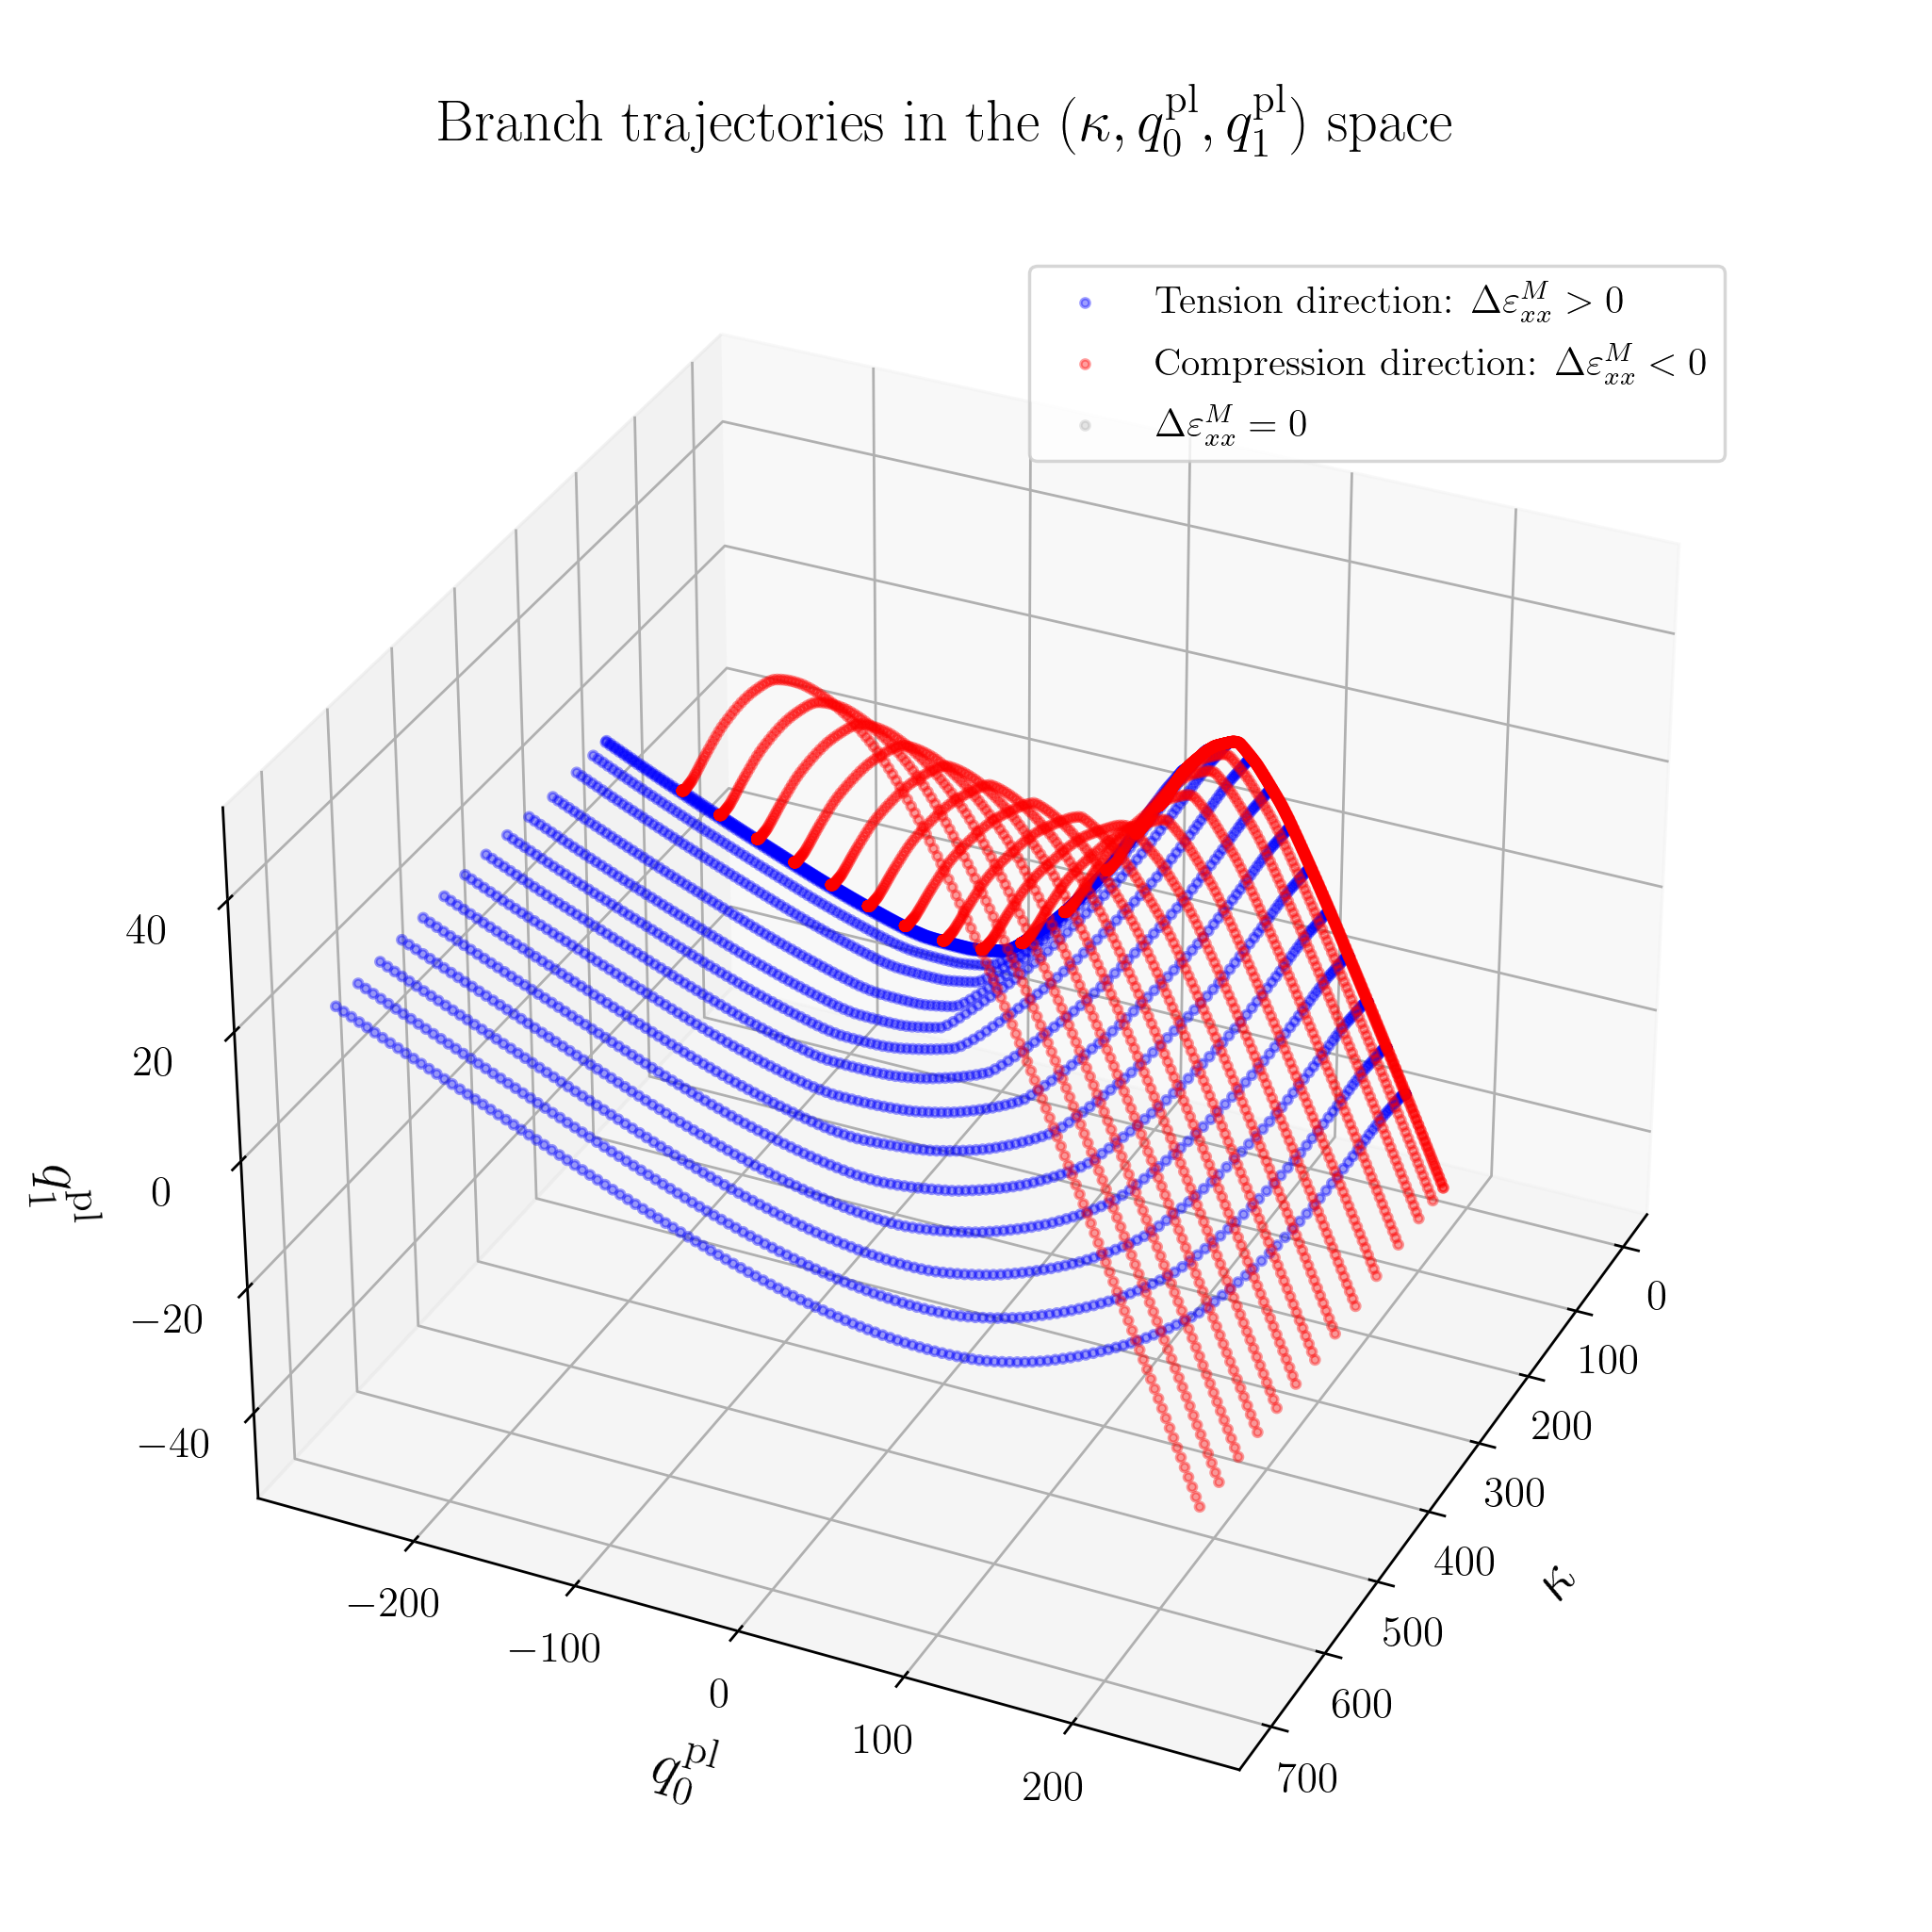
\includegraphics[width=0.32\textwidth]{latent_coordinate_story/branch_only_3d_kappa_qpl0_qpl1_view3.png}
\caption{Three views of the one-reversal trajectories in the $(\kappa,q^{\mathrm{pl}}_0,q^{\mathrm{pl}}_1)$ latent space.}
\label{fig:branch_3d_views}
\end{figure}

These visualizations reveal that the trajectories populate two smooth branchwise surfaces associated with the loading direction.

\subsection{Multi-Direction Test Trajectories}

Finally, we examine trajectories involving two loading reversals. These trajectories start in compression, reverse into tension, and then reverse again back into compression.

Figure~\ref{fig:branch_plus_test_xy_kappa_qpl0} shows these multi-direction trajectories superposed on the one-reversal branch cloud.

\begin{figure}[H]
\centering
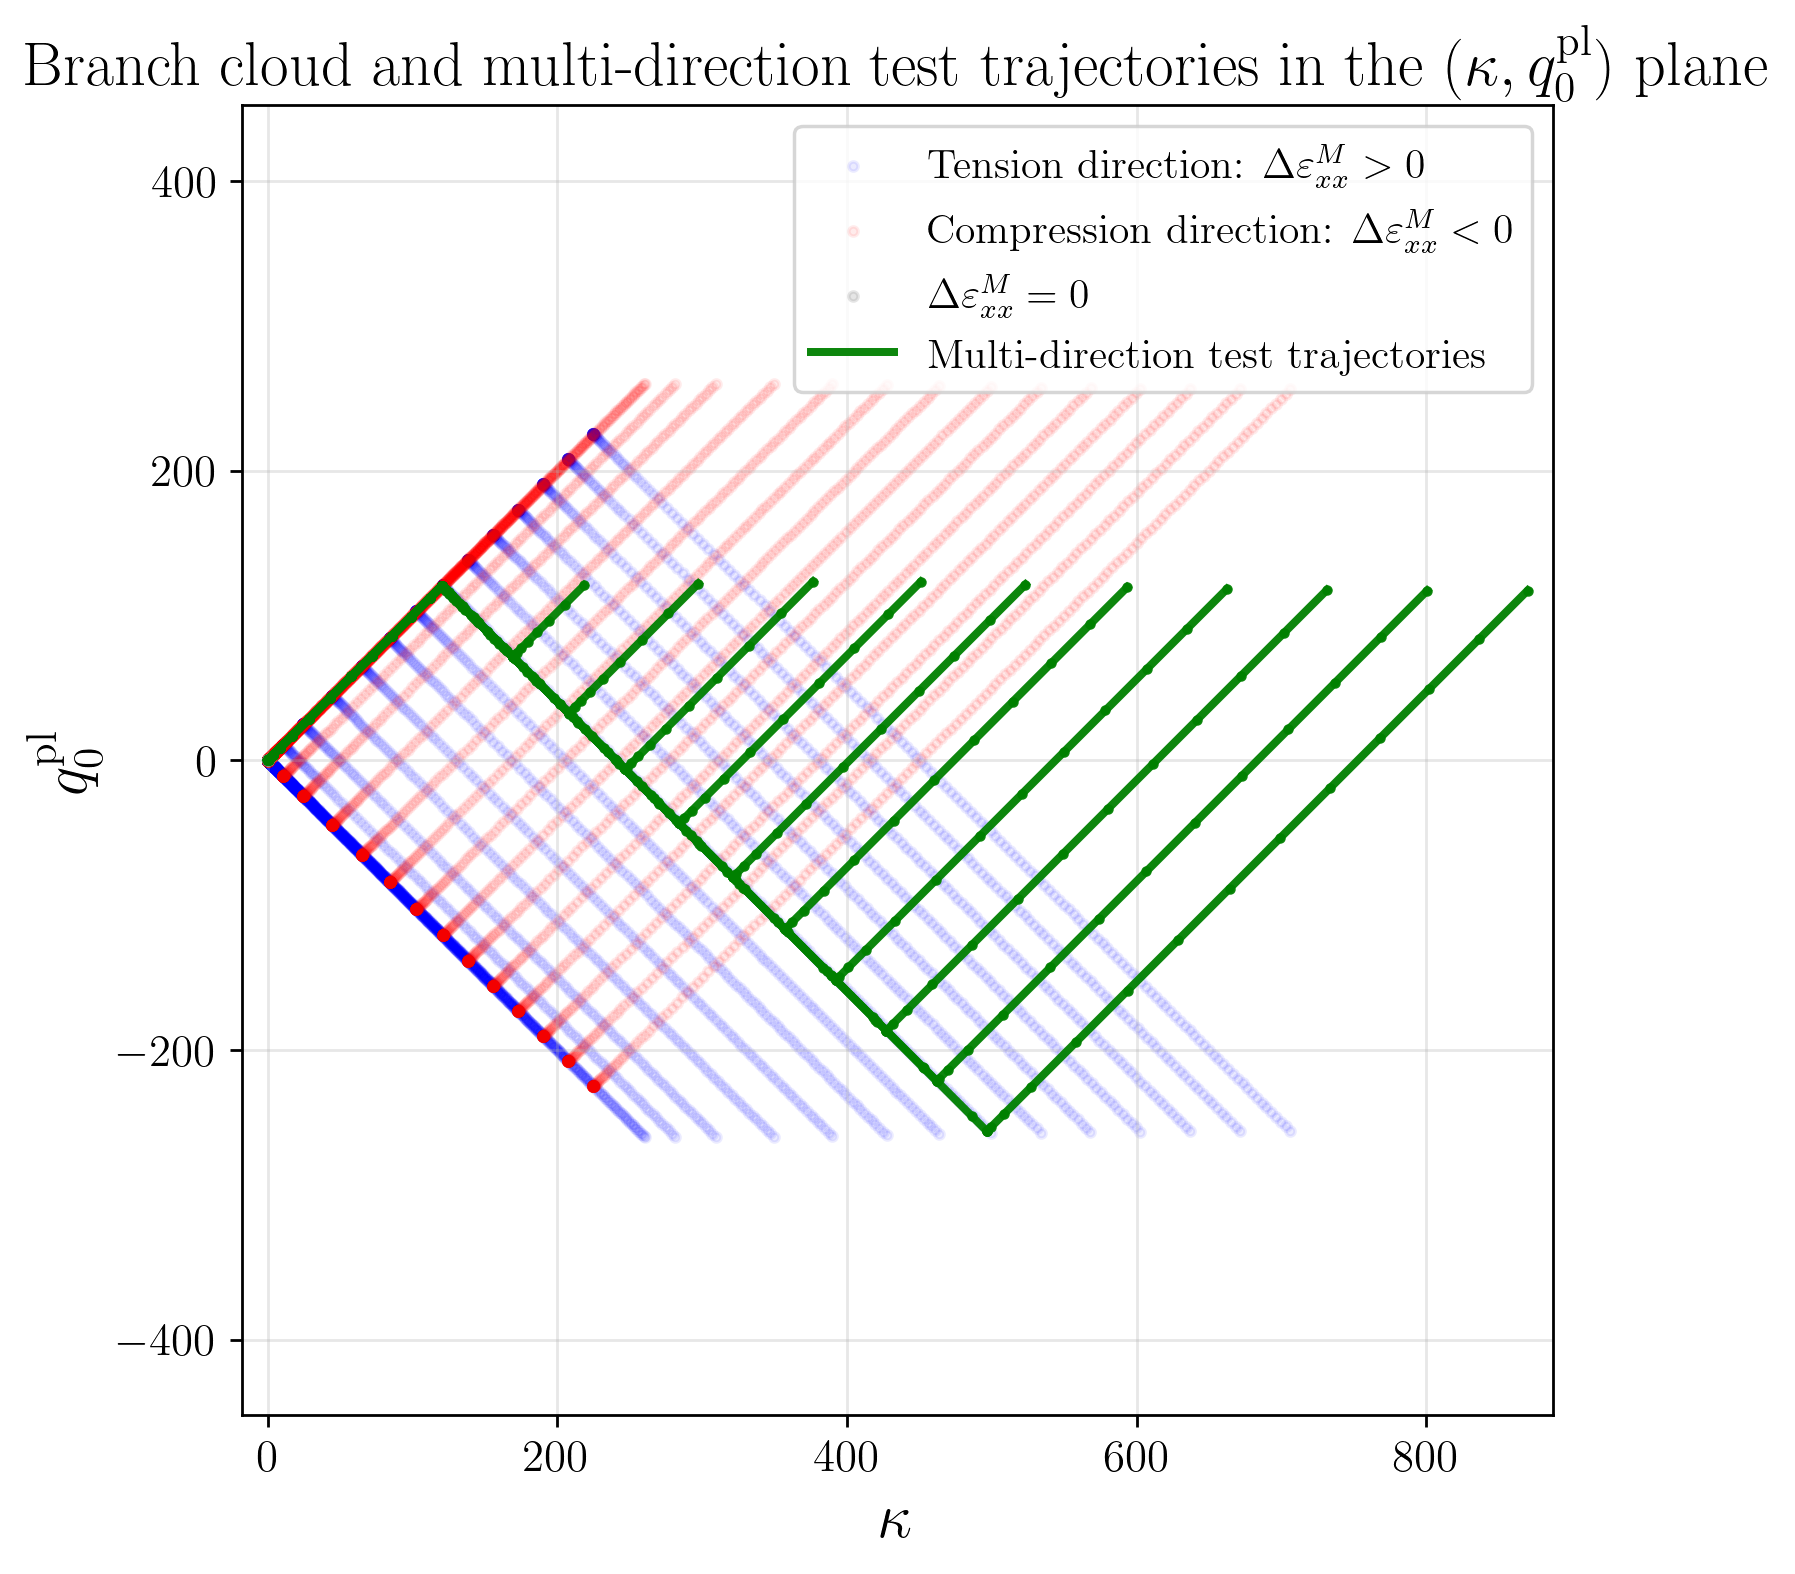
\includegraphics[width=0.70\textwidth]{latent_coordinate_story/branch_plus_test_xy_kappa_vs_qpl0.png}
\caption{Multi-direction trajectories in the $(\kappa,q^{\mathrm{pl}}_0)$ plane.}
\label{fig:branch_plus_test_xy_kappa_qpl0}
\end{figure}

The corresponding three-dimensional trajectories are shown in Figure~\ref{fig:branch_plus_test_3d}.

\begin{figure}[H]
\centering
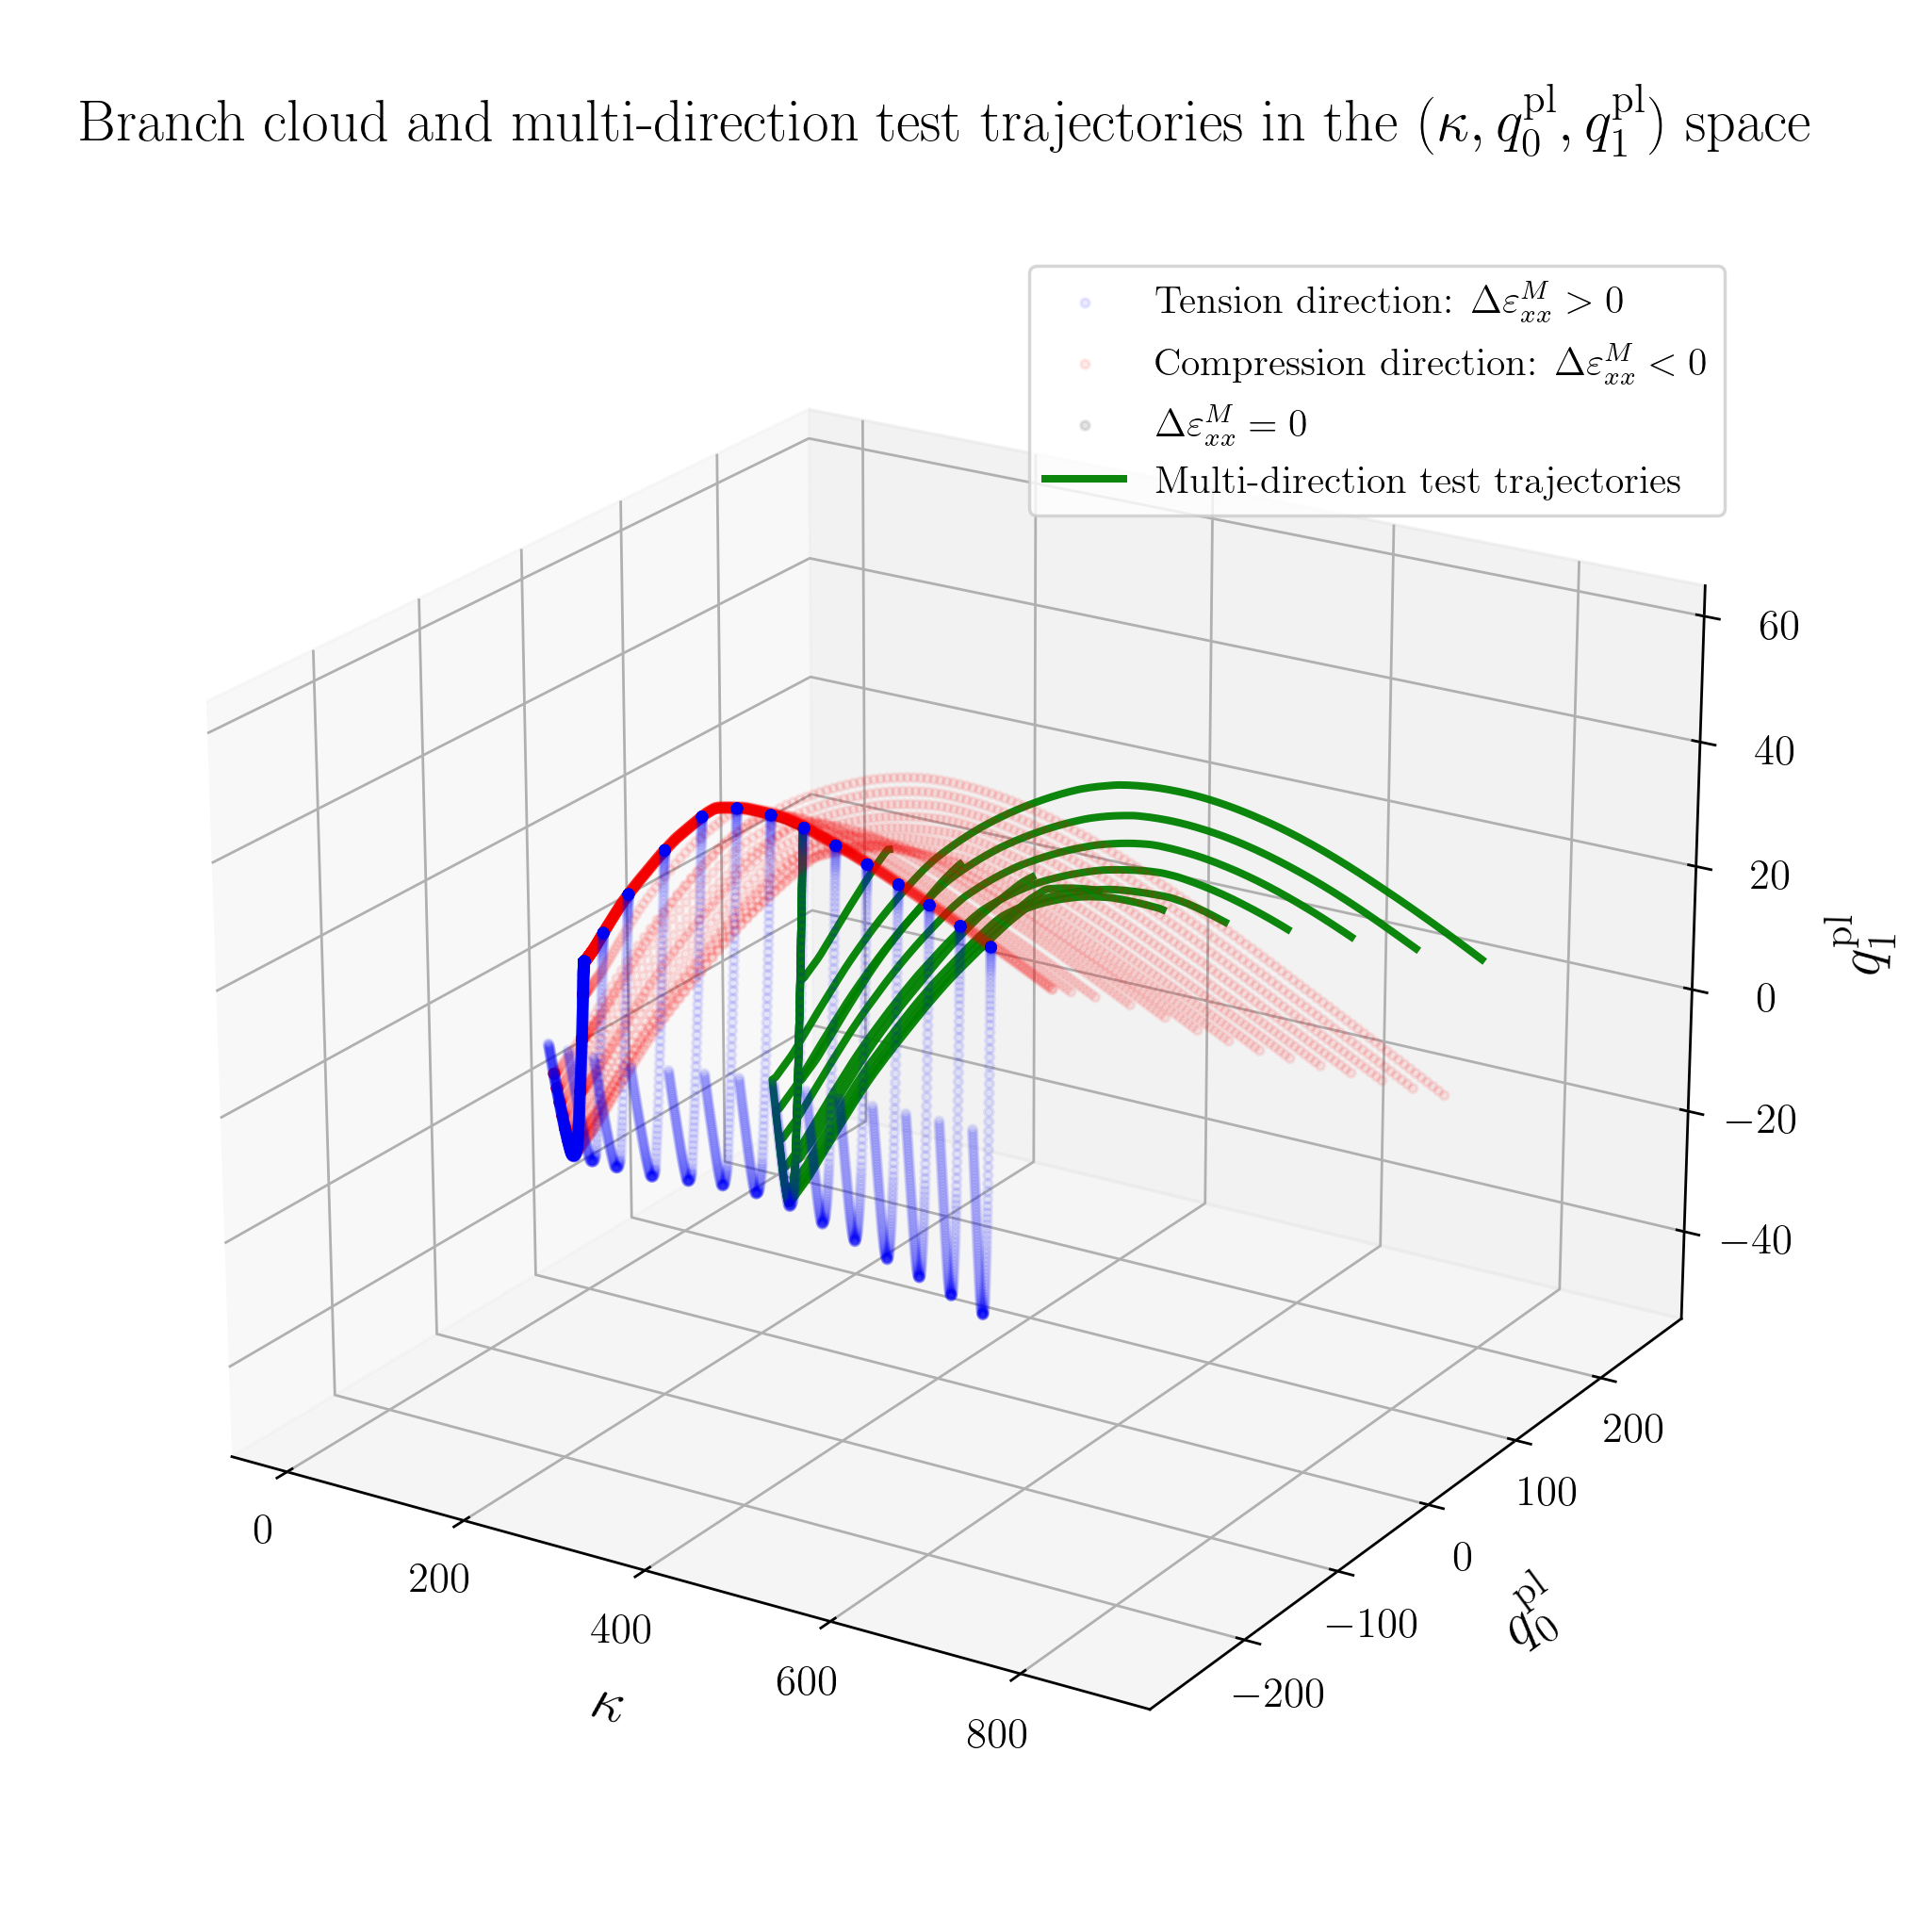
\includegraphics[width=0.32\textwidth]{latent_coordinate_story/branch_plus_test_3d_kappa_qpl0_qpl1_view1.png}
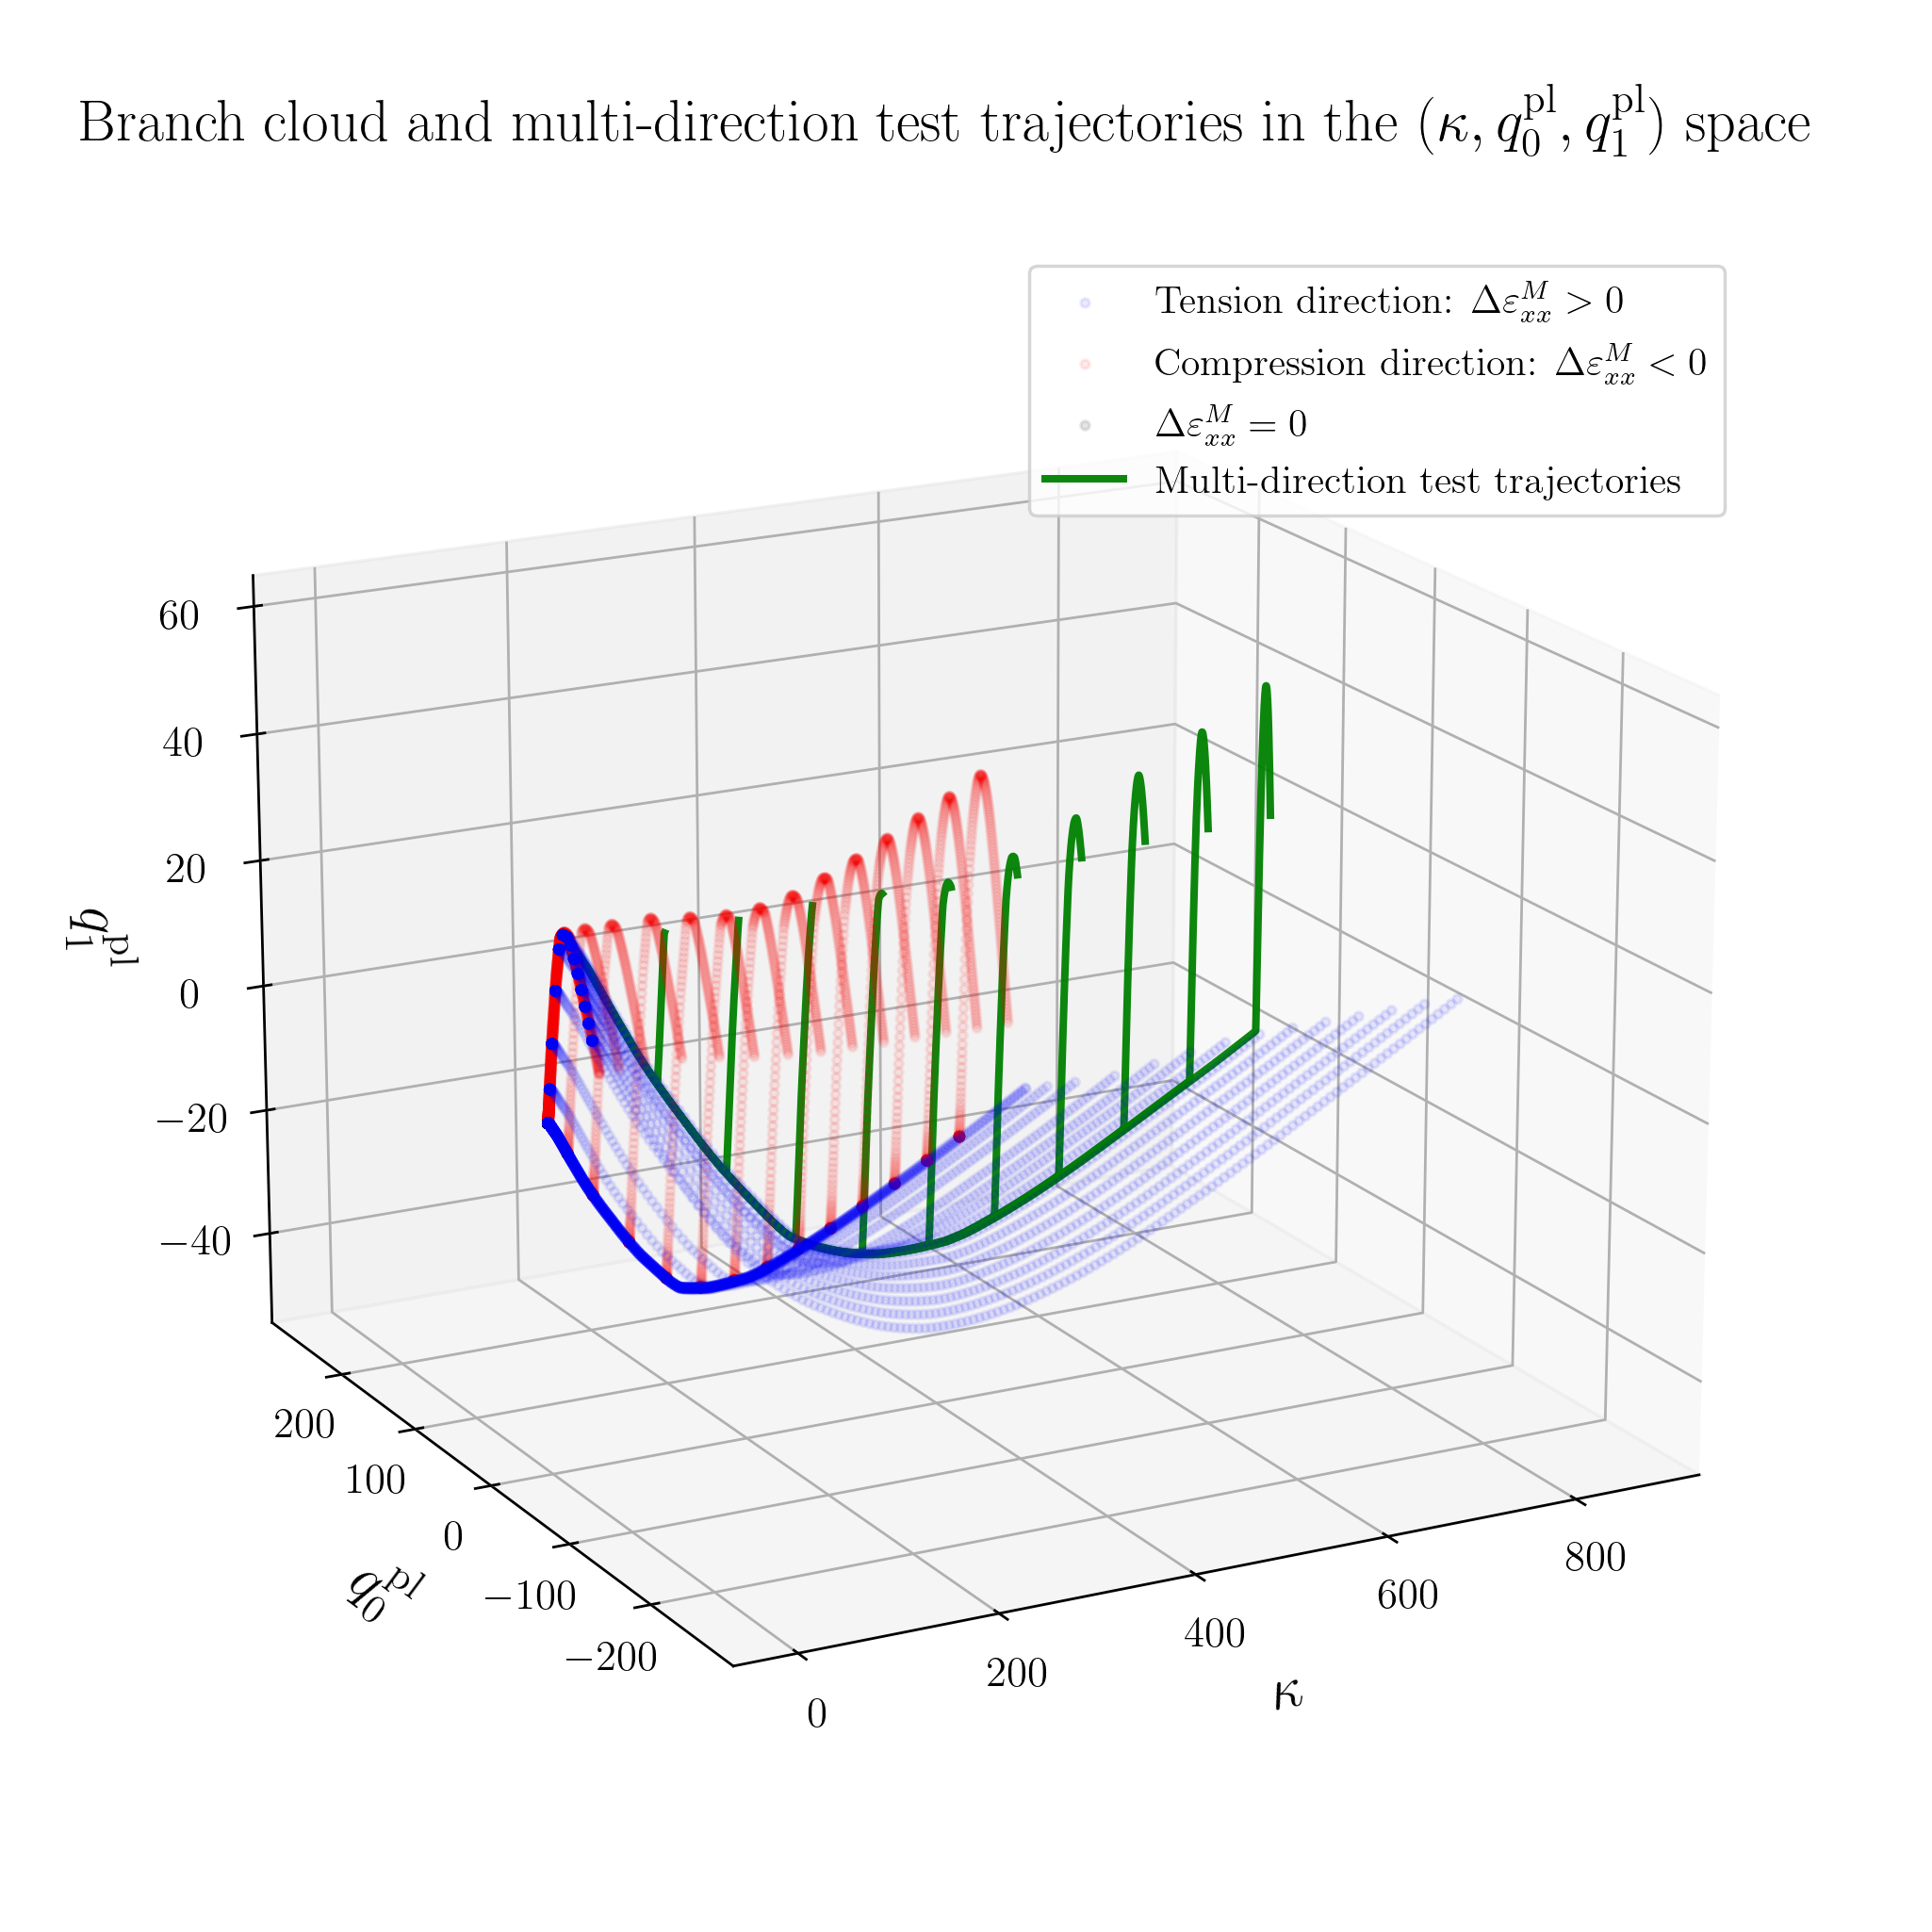
\includegraphics[width=0.32\textwidth]{latent_coordinate_story/branch_plus_test_3d_kappa_qpl0_qpl1_view2.png}
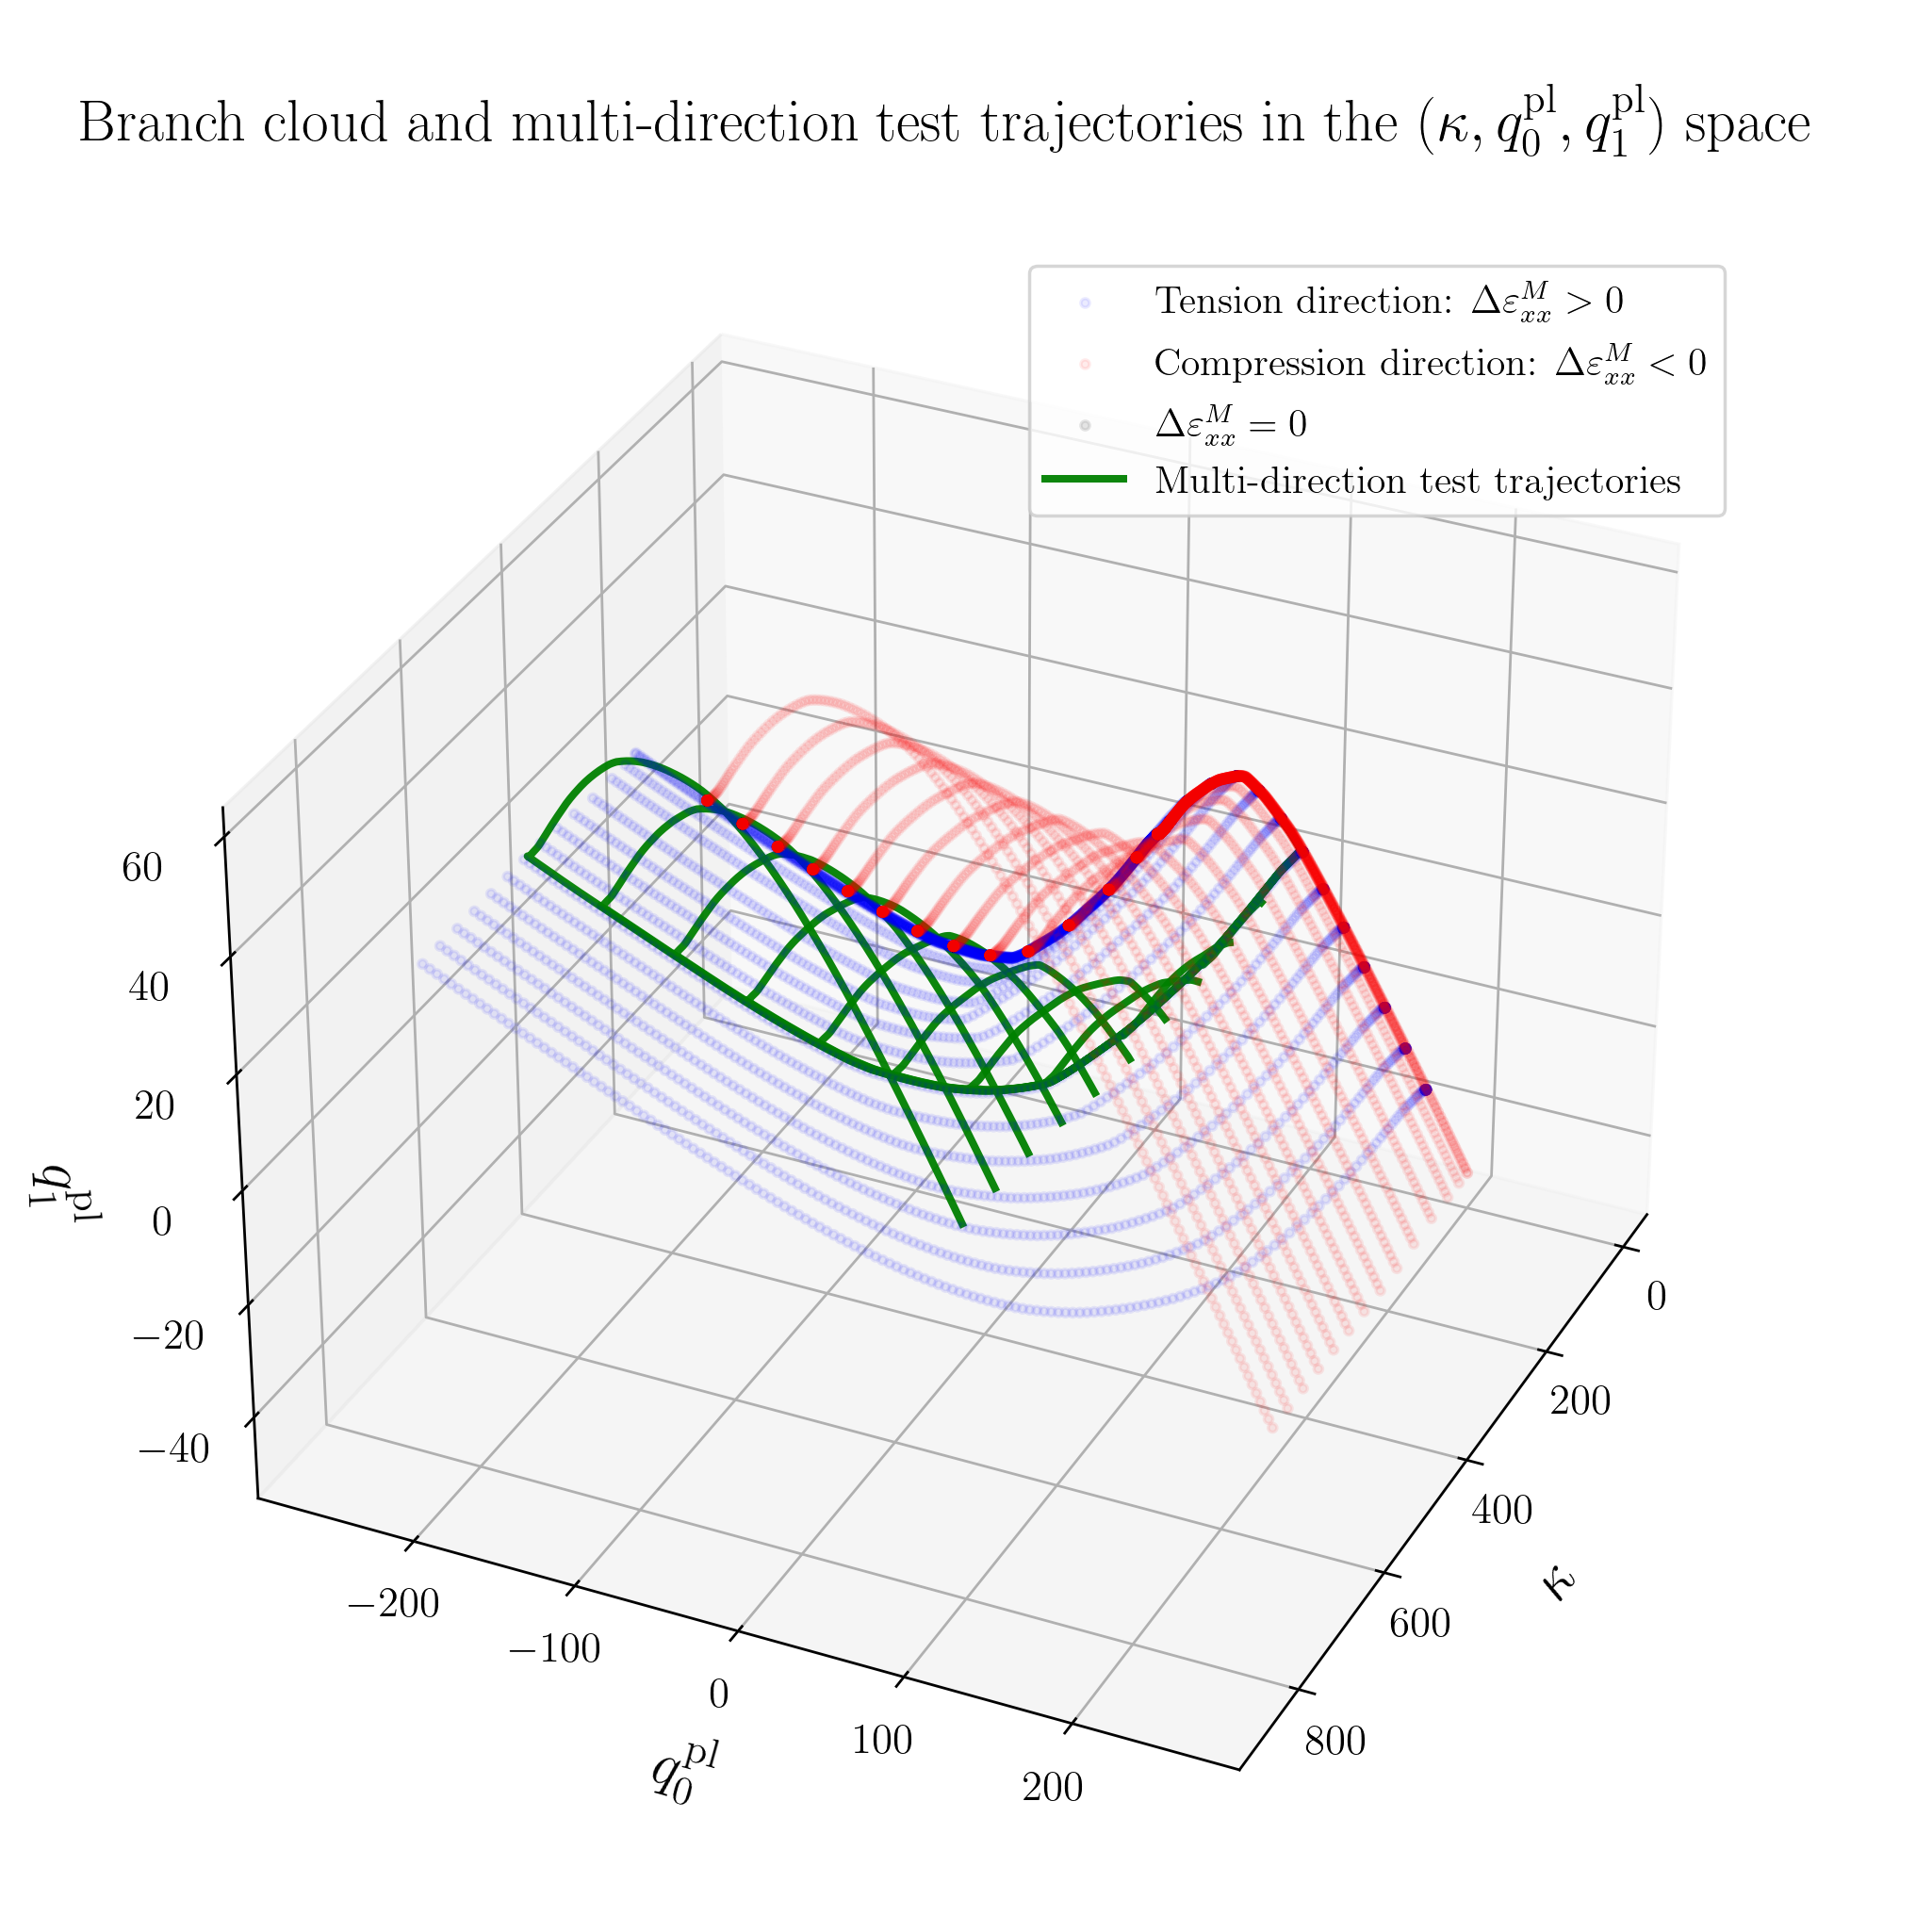
\includegraphics[width=0.32\textwidth]{latent_coordinate_story/branch_plus_test_3d_kappa_qpl0_qpl1_view3.png}
\caption{Three views of multi-direction test trajectories in latent space.}
\label{fig:branch_plus_test_3d}
\end{figure}

The green trajectories evolve within the same latent region structured by the one-reversal data. This observation suggests that the branchwise surfaces revealed by the simpler trajectories provide a meaningful geometric scaffold for more general loading histories.

These results motivate the construction of nonlinear branchwise regression surfaces depending on $(\kappa,q^{\mathrm{pl}}_0)$ and the loading direction. In the following section we show how such surfaces can be constructed using radial basis function interpolation and incorporated into the reduced-order model.

\subsection{Branchwise Nonlinear Approximation Using Radial Basis Functions}

The previous analysis revealed two important properties of the reduced plastic coordinates. 
First, the mapping between the leading plastic coordinate $q^{\mathrm{pl}}_0$ and the remaining coordinates is not single-valued. Second, the evolution clearly separates into two branches associated with the sign of the loading increment $\Delta \varepsilon_{xx}^{M}$. 

These observations suggest that a single nonlinear regression surface is insufficient to represent the plastic evolution. Instead, it is more appropriate to construct separate nonlinear approximations for each loading branch.

To this end we introduce two branchwise nonlinear mappings,
\[
q^{\mathrm{pl}}_1
=
\mathcal{N}^{(+)}(\kappa, q^{\mathrm{pl}}_0)
\qquad \text{for } \Delta \varepsilon_{xx}^{M} > 0,
\]

\[
q^{\mathrm{pl}}_1
=
\mathcal{N}^{(-)}(\kappa, q^{\mathrm{pl}}_0)
\qquad \text{for } \Delta \varepsilon_{xx}^{M} < 0,
\]

where $\kappa$ is the accumulated latent variable introduced previously. 
The two functions $\mathcal{N}^{(+)}$ and $\mathcal{N}^{(-)}$ are approximated using radial basis function (RBF) interpolation constructed from reduced-order model trajectories.

More precisely, the data used to construct the regression surfaces are obtained from the validation ROM simulations introduced earlier. For each trajectory the reduced coordinates $(\kappa,q^{\mathrm{pl}}_0,q^{\mathrm{pl}}_1)$ are computed from the projected displacement fields, and each state is assigned to a branch according to the sign of the macroscopic strain increment $\Delta \varepsilon_{xx}^{M}$.

The resulting point clouds in the latent space $(\kappa,q^{\mathrm{pl}}_0,q^{\mathrm{pl}}_1)$ are shown in Figure~\ref{fig:stage3_rbf_surfaces}. 
Points corresponding to positive loading increments ($\Delta \varepsilon_{xx}^{M}>0$) are shown in blue, while points corresponding to negative increments ($\Delta \varepsilon_{xx}^{M}<0$) are shown in red. 

Using these data sets, two independent RBF interpolants are constructed, each approximating the relation between $(\kappa,q^{\mathrm{pl}}_0)$ and $q^{\mathrm{pl}}_1$ for one loading direction. The resulting nonlinear surfaces are also displayed in Figure~\ref{fig:stage3_rbf_surfaces}. 

Several observations can be made from this visualization. 
First, the latent trajectories generated by the reduced-order simulations lie close to well-defined two-dimensional manifolds in the three-dimensional latent space. 
Second, the two manifolds are clearly separated according to the loading direction. 
Finally, the RBF surfaces provide a smooth approximation of these manifolds over the domain spanned by the available trajectories.

These branchwise nonlinear approximations therefore provide a compact representation of the plastic evolution in the latent space. However, they do not yet fully resolve the problem of path dependence. 
In particular, during complex loading histories the state of the system may move between regions associated with different loading directions. 

This observation motivates the next step of the construction, where the evolution of the latent state will be interpreted geometrically and used to define a history-aware mechanism for evaluating the nonlinear approximation along arbitrary trajectories.

\begin{figure}[H]
\centering
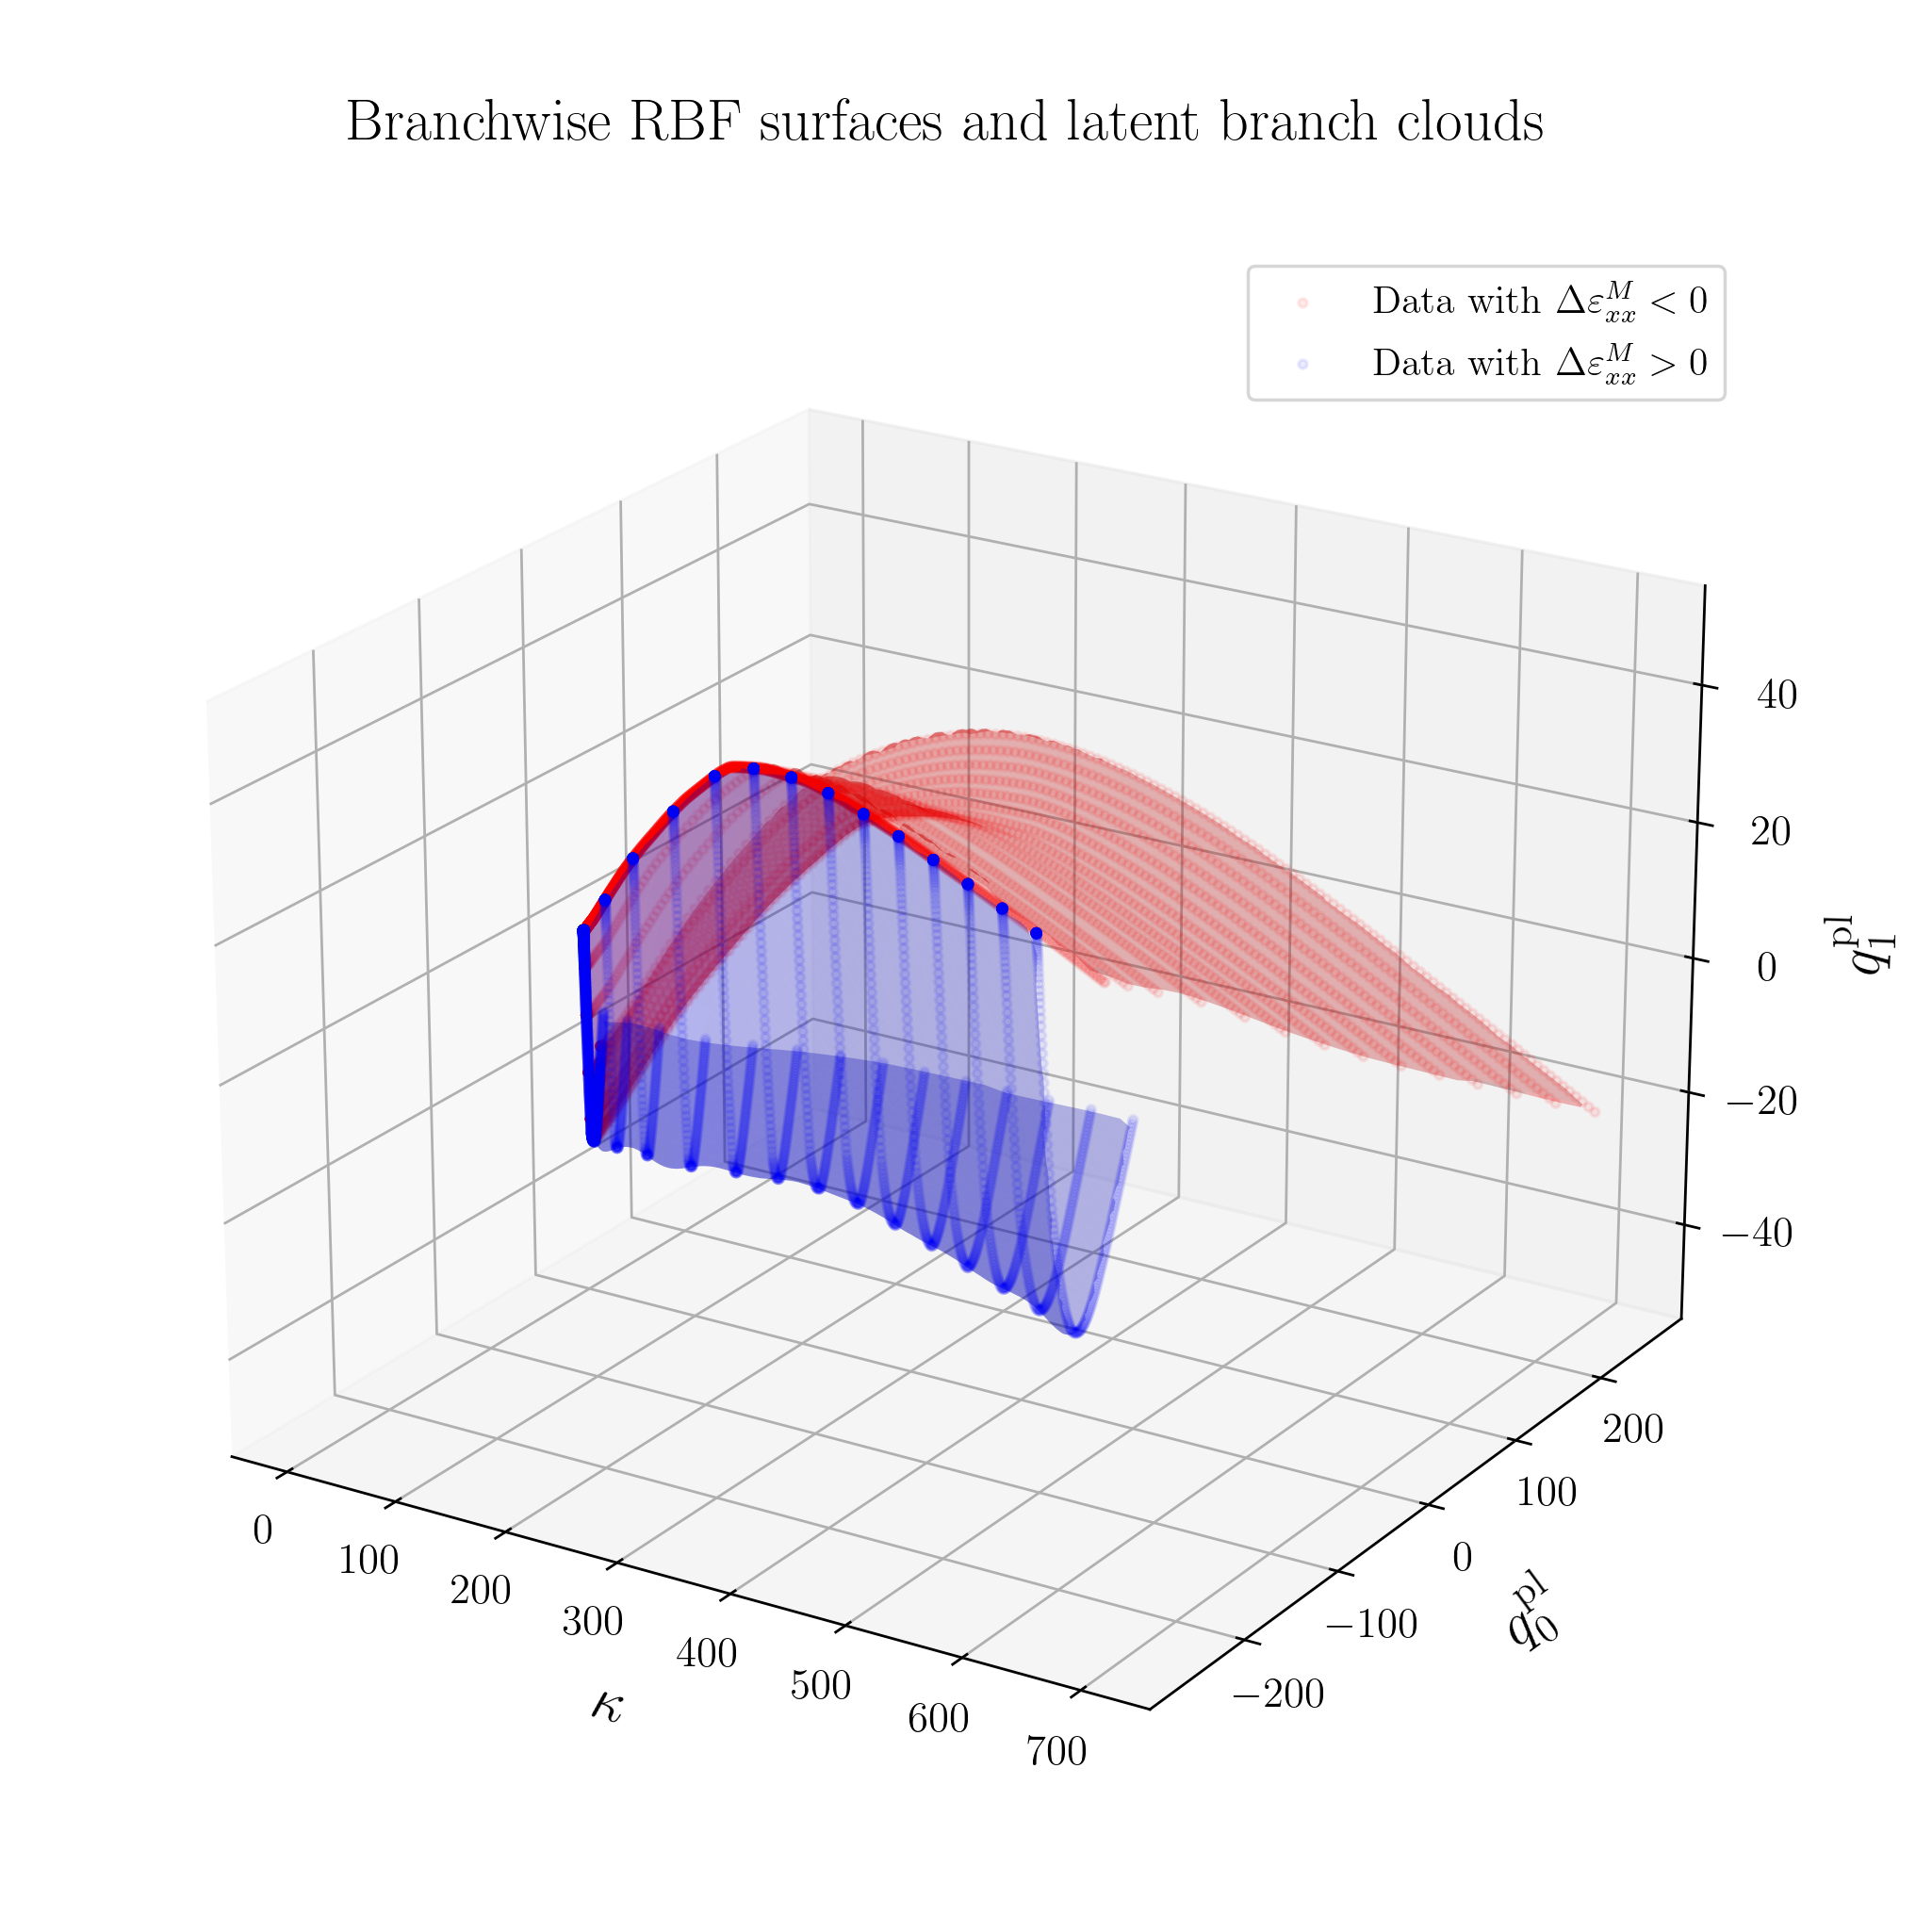
\includegraphics[width=0.32\textwidth]{stage3_two_branch_rbf_story/stage3_surfaces_with_clouds_view1.png}
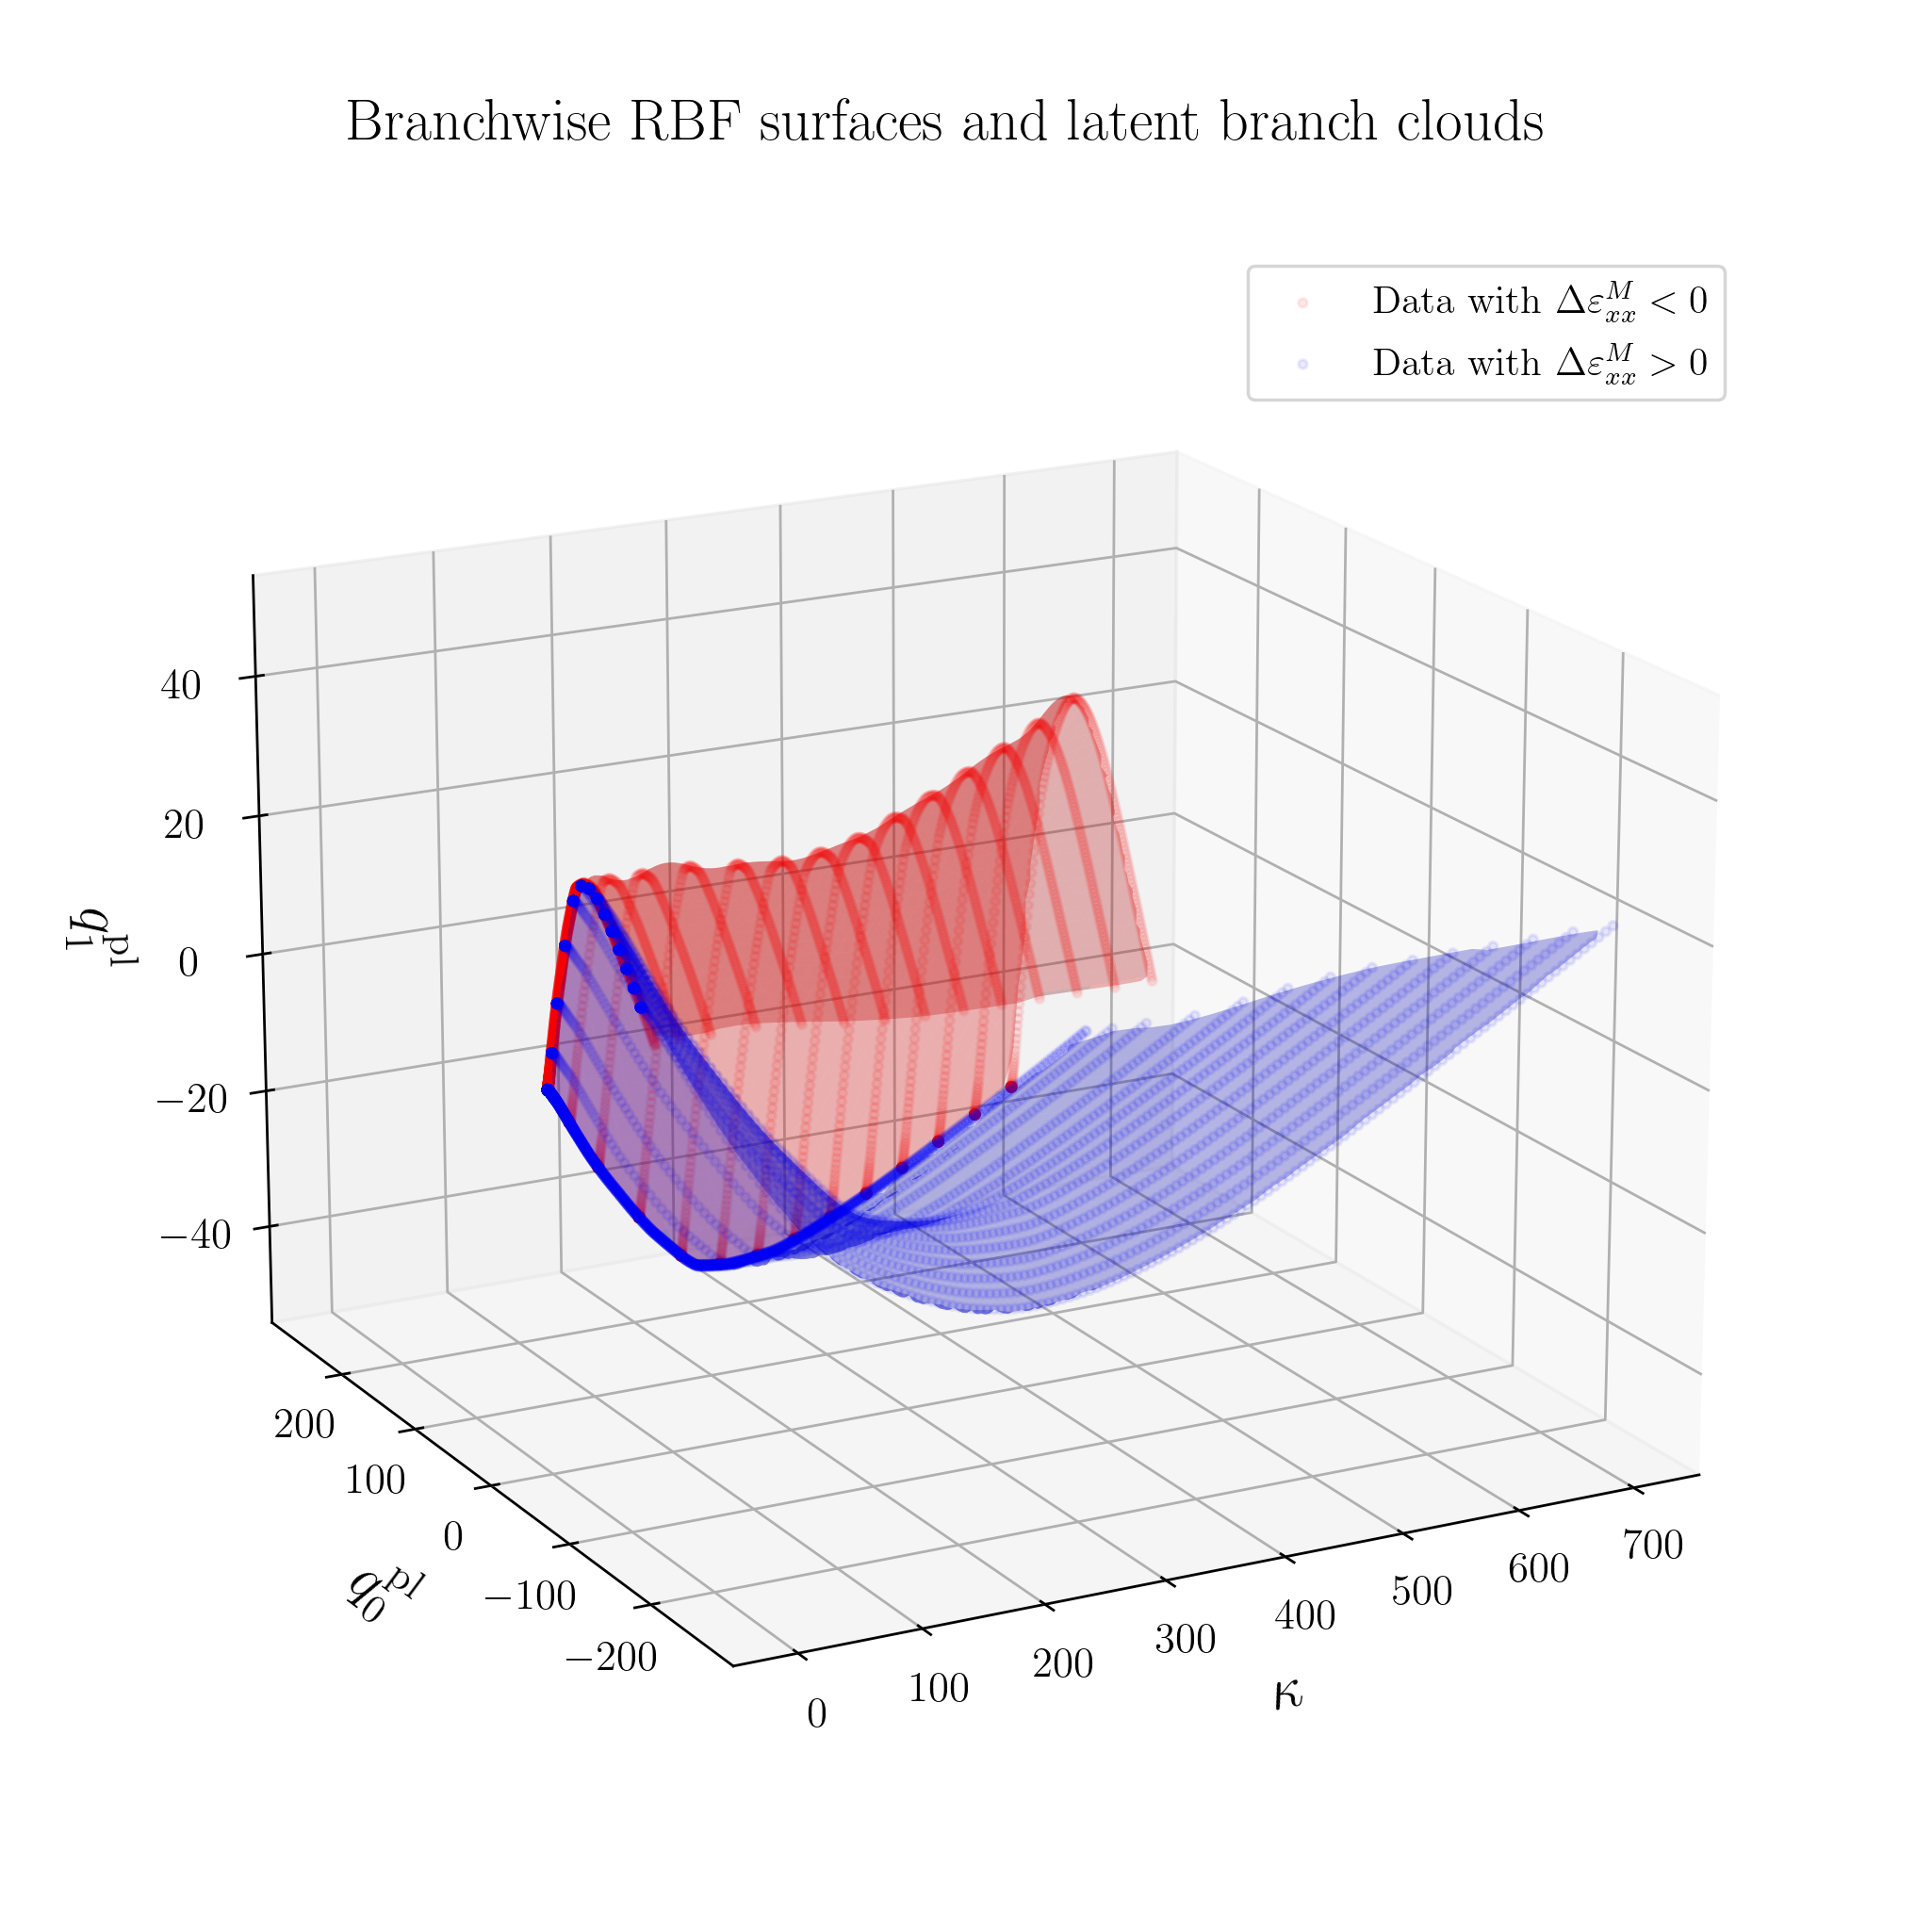
\includegraphics[width=0.32\textwidth]{stage3_two_branch_rbf_story/stage3_surfaces_with_clouds_view2.png}
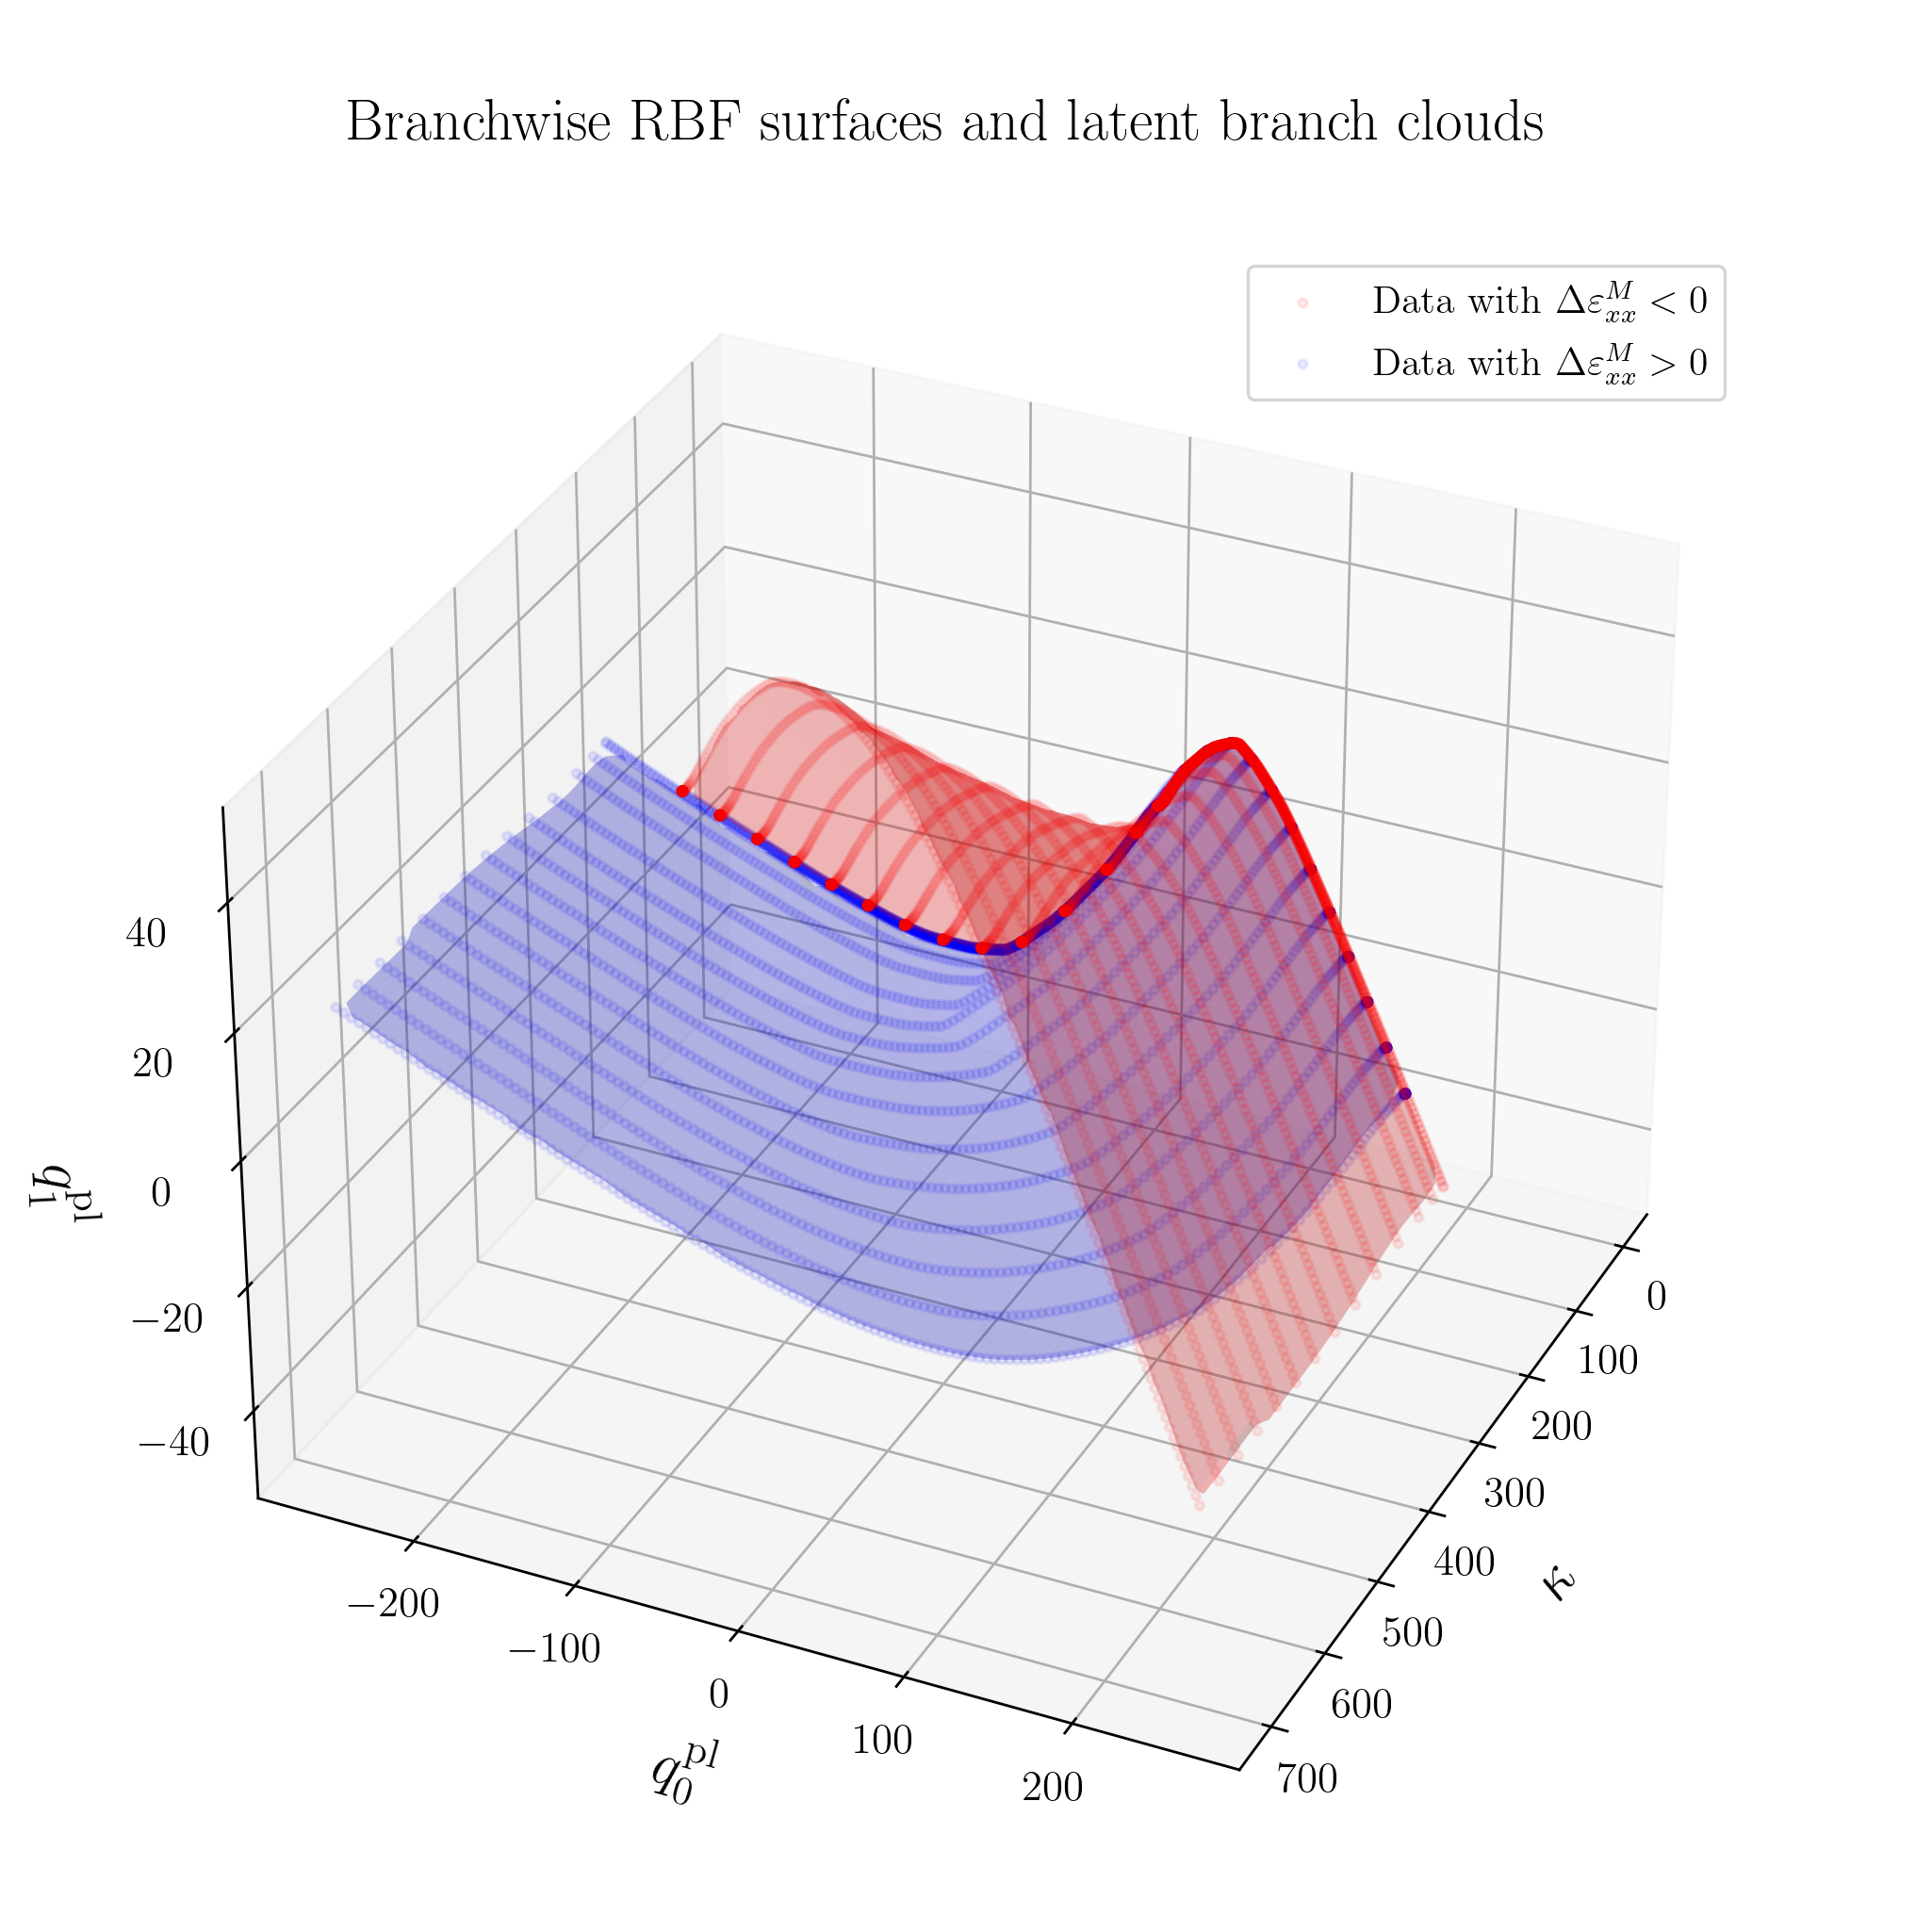
\includegraphics[width=0.32\textwidth]{stage3_two_branch_rbf_story/stage3_surfaces_with_clouds_view3.png}
\caption{Branchwise nonlinear approximation of the latent plastic dynamics. 
The red and blue point clouds correspond to states obtained from ROM simulations with $\Delta \varepsilon_{xx}^{M}<0$ and $\Delta \varepsilon_{xx}^{M}>0$, respectively. 
The semi-transparent surfaces represent radial basis function approximations of the relation between $(\kappa,q^{\mathrm{pl}}_0)$ and $q^{\mathrm{pl}}_1$ for each loading branch.}
\label{fig:stage3_rbf_surfaces}
\end{figure}

\section{Branchwise Surface Transport with Boundary Projection}

The purpose of this section is to define the transported two-branch latent surrogate in a precise geometric form. The goal is not to introduce yet another nonlinear regression model, but to explain how two previously learned branchwise latent surfaces can be reused along trajectories with multiple loading reversals.

The key point is the following. The offline branchwise surfaces remain fixed after training. Path dependence is introduced online through a transport state that shifts the in-plane latent frame and re-anchors the active branch vertically. The resulting construction allows the surrogate to remain consistent across changes of loading direction without redefining the underlying latent maps.

The section is organized deductively. We first define the latent variables and the branchwise latent surfaces. We then introduce the transport state, explain how projections onto the transported wedge boundaries are computed, and finally describe the online update mechanism at initialization, during smooth branch evolution, and at switching events.

\subsection{Latent coordinates and vector-valued closure}

Let the reduced displacement approximation be partitioned into elastic and plastic contributions, and let
\begin{equation}
\mathbf{q}^{\mathrm{pl}}
=
\begin{bmatrix}
q^{\mathrm{pl}}_0 &
q^{\mathrm{pl}}_1 &
\cdots &
q^{\mathrm{pl}}_{r_{\mathrm{pl}}-1}
\end{bmatrix}^{T}
\end{equation}
denote the vector of plastic reduced coordinates. The latent coordinates used in the transported construction are obtained by projection of the microscopic displacement field,
\begin{equation}
q^{\mathrm{pl}}_0 = \mathbf{w}_0^{T}\mathbf{u},
\qquad
q^{\mathrm{pl}}_j = \mathbf{w}_j^{T}\mathbf{u},
\qquad
j=1,\dots,r_{\mathrm{pl}}-1,
\label{eq:qpl_projection_transport_ts_ref}
\end{equation}
where \(\mathbf{u}\) is the microscopic displacement vector and \(\mathbf{w}_j\) are the corresponding projection operators.

Although the figures only display \(q^{\mathrm{pl}}_1\), the transported closure is intended for the whole target vector
\begin{equation}
\mathbf{q}^{\mathrm{pl}}_{\mathrm{tgt}}
=
\begin{bmatrix}
q^{\mathrm{pl}}_1 &
q^{\mathrm{pl}}_2 &
\cdots &
q^{\mathrm{pl}}_{r_{\mathrm{pl}}-1}
\end{bmatrix}^{T}.
\label{eq:qpl_target_vector_transport_ts_ref}
\end{equation}
Therefore, the visualizations are scalar only for exposition. The final construction is vector-valued.

The main difficulty is that the target coordinates cannot be represented accurately as a single-valued function of \(q^{\mathrm{pl}}_0\) alone. To enrich the state, we introduce the cumulative variable
\begin{equation}
\kappa_0 = 0,
\qquad
\kappa_n
=
\sum_{m=1}^{n}
\left|
q^{\mathrm{pl}}_0{}^{(m)}
-
q^{\mathrm{pl}}_0{}^{(m-1)}
\right|.
\label{eq:kappa_definition_transport_ts_ref}
\end{equation}
The pair \((\kappa,q^{\mathrm{pl}}_0)\) provides the two-dimensional latent description on which the branchwise surrogate is built.

\subsection{Change of variables to the quadrant coordinates \texorpdfstring{$(t,s)$}{(t,s)}}

A more transparent geometric interpretation is obtained through the variables
\begin{equation}
t
=
\frac{\kappa + q^{\mathrm{pl}}_0}{2},
\qquad
s
=
\frac{\kappa - q^{\mathrm{pl}}_0}{2}.
\label{eq:ts_definition_transport_ref}
\end{equation}
Equivalently,
\begin{equation}
\kappa = t+s,
\qquad
q^{\mathrm{pl}}_0 = t-s.
\label{eq:kappa_q0_from_ts_transport_ref}
\end{equation}

These variables separate the accumulated positive and negative excursions of the leading plastic coordinate. In particular,
\begin{itemize}
\item \(t\) is associated with motion toward \(q^{\mathrm{pl}}_0>0\),
\item \(s\) is associated with motion toward \(q^{\mathrm{pl}}_0<0\).
\end{itemize}

Since \(\kappa\) is defined as a cumulative absolute increment of \(q^{\mathrm{pl}}_0\), one always has
\begin{equation}
|q^{\mathrm{pl}}_0| \le \kappa,
\label{eq:wedge_constraint_transport_ts_ref}
\end{equation}
which is equivalent to
\begin{equation}
t \ge 0,
\qquad
s \ge 0.
\label{eq:ts_nonnegative_transport_ref}
\end{equation}

Therefore, the admissible domain in the \((\kappa,q^{\mathrm{pl}}_0)\) plane is a wedge, whereas in the \((t,s)\) variables it becomes the first quadrant. This reformulation is useful because switching will later be interpreted as projection onto the transported axes of that quadrant.

The boundaries of the reference wedge are
\begin{equation}
\Gamma_0^{+}:\quad q^{\mathrm{pl}}_0=\kappa,
\qquad
\Gamma_0^{-}:\quad q^{\mathrm{pl}}_0=-\kappa,
\label{eq:reference_wedge_transport_ts_ref}
\end{equation}
which correspond to
\begin{equation}
\Gamma_0^{+} \iff s=0,
\qquad
\Gamma_0^{-} \iff t=0.
\label{eq:wedge_walls_ts_transport_ref}
\end{equation}

Figure~\ref{fig:transport_stageA_xy_support_ts_ref} shows the latent support and the ROM path in the \((\kappa,q^{\mathrm{pl}}_0)\) plane, together with the \(t\)- and \(s\)-directions. In this representation the wedge geometry is explicit. The same information may be interpreted in the transformed \((t,s)\) coordinates, where the wedge becomes the first quadrant.

\begin{figure}[H]
\centering
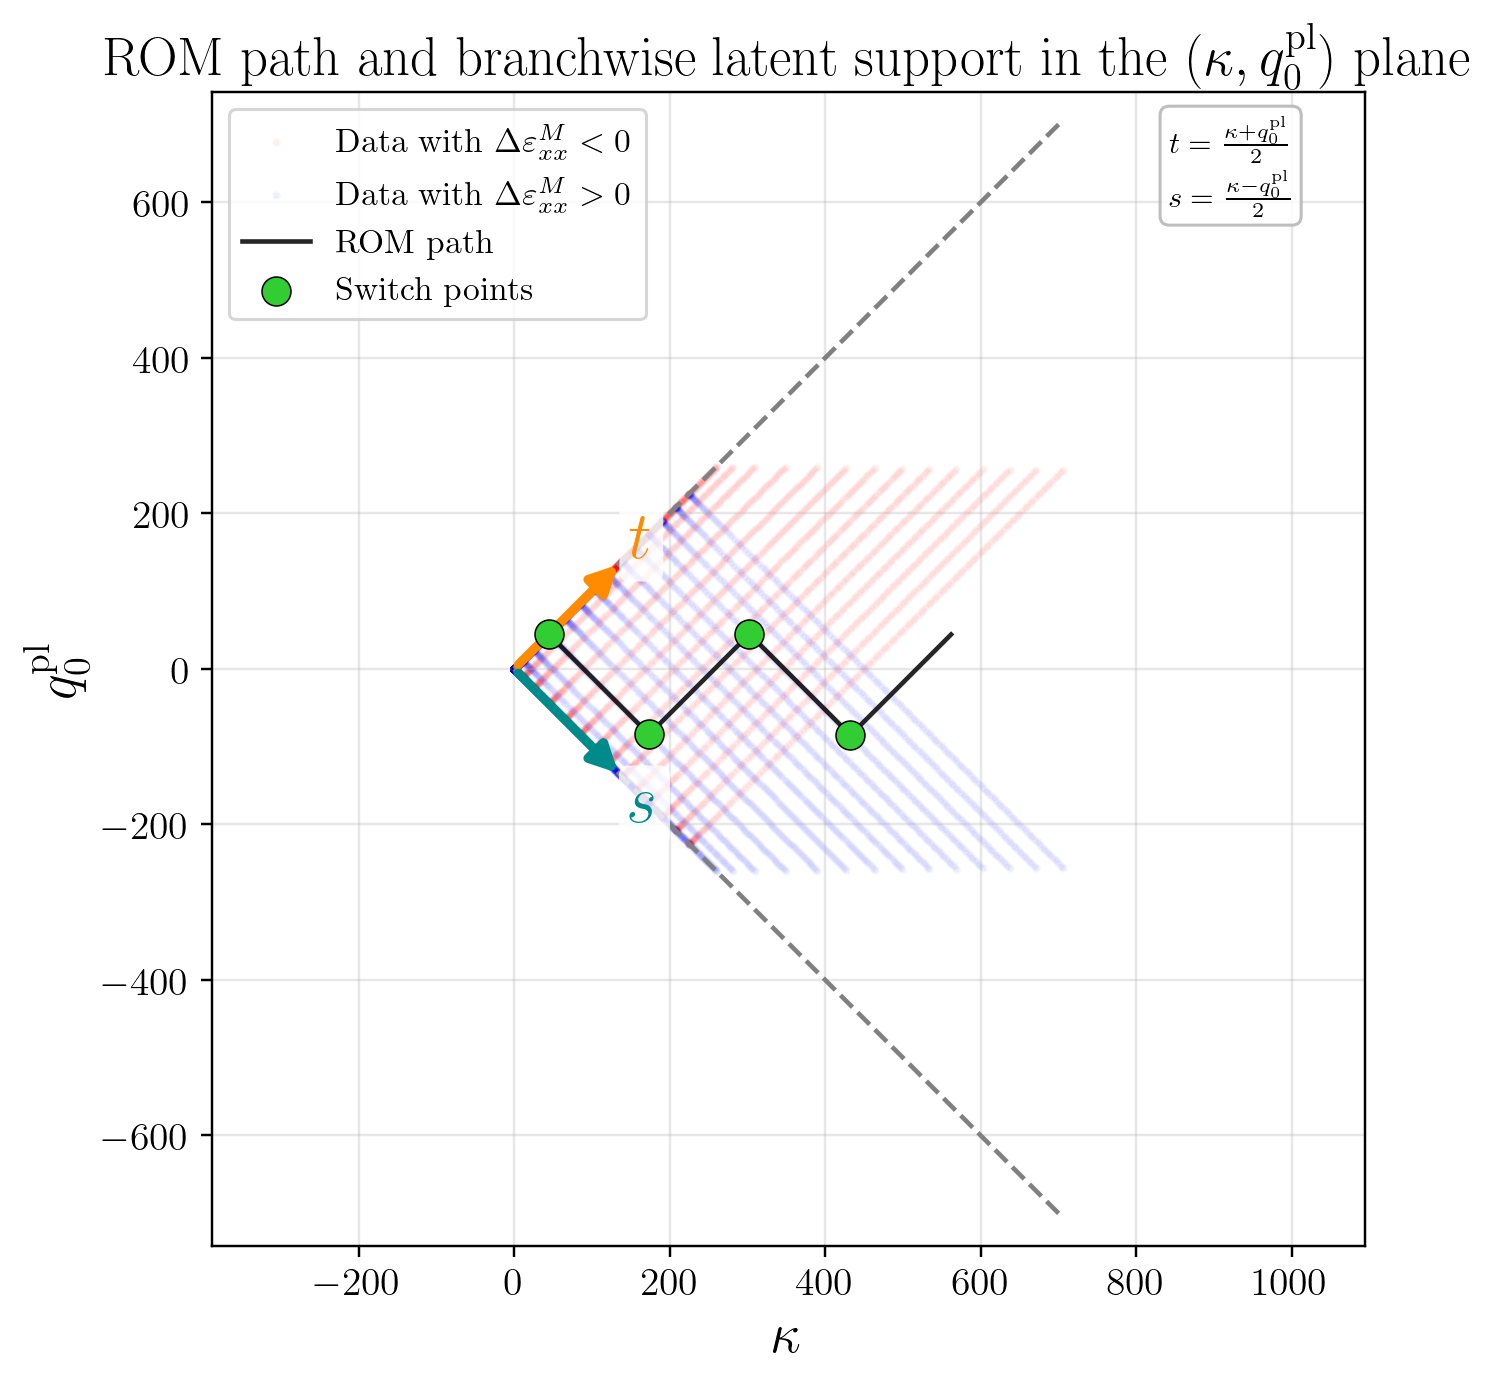
\includegraphics[width=0.74\textwidth]{two_surface_switch_with_boundary_projection_transport/stageA_xy_support_and_path.png}
\caption{ROM path and branchwise latent support in the \((\kappa,q^{\mathrm{pl}}_0)\) plane. The gray dashed wedge boundaries correspond to the axes of the equivalent \((t,s)\) quadrant.}
\label{fig:transport_stageA_xy_support_ts_ref}
\end{figure}

\subsection{Offline branchwise latent surfaces}

The ROM data reveals that the latent dynamics separates into two branches according to the sign of the macroscopic strain increment \(\Delta \varepsilon_{xx}^{M}\). We therefore define two branchwise vector-valued maps
\begin{align}
\mathbf{q}^{\mathrm{pl}}_{\mathrm{tgt}}
&=
\mathcal{N}^{-}(\kappa,q^{\mathrm{pl}}_0),
\qquad
\text{for } \Delta \varepsilon_{xx}^{M}<0,
\label{eq:Nminus_vector_transport_ref}
\\
\mathbf{q}^{\mathrm{pl}}_{\mathrm{tgt}}
&=
\mathcal{N}^{+}(\kappa,q^{\mathrm{pl}}_0),
\qquad
\text{for } \Delta \varepsilon_{xx}^{M}>0.
\label{eq:Nplus_vector_transport_ref}
\end{align}

Using \eqref{eq:kappa_q0_from_ts_transport_ref}, these may be written equivalently as
\begin{align}
\mathbf{q}^{\mathrm{pl}}_{\mathrm{tgt}}
&=
\widehat{\mathcal{N}}^{-}(t,s)
:=
\mathcal{N}^{-}(t+s,t-s),
\label{eq:Nminus_ts_transport_ref}
\\
\mathbf{q}^{\mathrm{pl}}_{\mathrm{tgt}}
&=
\widehat{\mathcal{N}}^{+}(t,s)
:=
\mathcal{N}^{+}(t+s,t-s).
\label{eq:Nplus_ts_transport_ref}
\end{align}

These maps are learned offline from branch-split ROM data. Their shape remains fixed afterwards. The online construction does not deform these surfaces. Instead, it changes the frame in which they are evaluated.

This distinction is central. The method does not update the regression model itself. It updates only the transport state used to position the active branch relative to the current trajectory.

\subsection{What is fixed and what is transported}

It is useful to separate clearly the offline and online ingredients.

\paragraph{Fixed offline objects.}
The learned branchwise maps
\[
\mathcal{N}^{-},
\qquad
\mathcal{N}^{+},
\]
or equivalently
\[
\widehat{\mathcal{N}}^{-},
\qquad
\widehat{\mathcal{N}}^{+},
\]
remain fixed once trained.

\paragraph{Transported online objects.}
During trajectory evolution,
\begin{itemize}
\item the in-plane latent frame is translated,
\item each branch receives its own vertical correction in the target-coordinate space.
\end{itemize}

Thus, the online mechanism is a geometric transport of fixed offline surfaces. It is not a retraining step.

\subsection{Transport state in the \texorpdfstring{$(\kappa,q^{\mathrm{pl}}_0)$}{(kappa,qpl0)} frame}

Let
\[
\Delta K,
\qquad
\Delta Q_0
\]
denote the current in-plane translation in the \((\kappa,q^{\mathrm{pl}}_0)\) plane. In addition, let
\[
\Delta \mathbf{Q}_{\mathrm{tgt}}^{-},
\qquad
\Delta \mathbf{Q}_{\mathrm{tgt}}^{+}
\]
denote the branchwise vertical offsets in the target-coordinate space. These vectors have the same dimension as \(\mathbf{q}^{\mathrm{pl}}_{\mathrm{tgt}}\).

The transported branch surfaces are then defined by
\begin{align}
\widetilde{\mathcal{N}}^{-}(\kappa,q^{\mathrm{pl}}_0)
&=
\mathcal{N}^{-}(\kappa-\Delta K,\;q^{\mathrm{pl}}_0-\Delta Q_0)
+
\Delta \mathbf{Q}_{\mathrm{tgt}}^{-},
\label{eq:Nminus_transported_vector_transport_ref}
\\
\widetilde{\mathcal{N}}^{+}(\kappa,q^{\mathrm{pl}}_0)
&=
\mathcal{N}^{+}(\kappa-\Delta K,\;q^{\mathrm{pl}}_0-\Delta Q_0)
+
\Delta \mathbf{Q}_{\mathrm{tgt}}^{+}.
\label{eq:Nplus_transported_vector_transport_ref}
\end{align}

Only the first component, namely the prediction of \(q^{\mathrm{pl}}_1\), is visualized in the figures. The formulas themselves apply to the complete target vector.

\subsection{Equivalent transport state in the \texorpdfstring{$(t,s)$}{(t,s)} frame}

The same in-plane translation can be written in the transformed coordinates. Define
\begin{equation}
\Delta t
=
\frac{\Delta K+\Delta Q_0}{2},
\qquad
\Delta s
=
\frac{\Delta K-\Delta Q_0}{2}.
\label{eq:delta_ts_from_deltaKQ_transport_ref}
\end{equation}
Then
\begin{equation}
\Delta K = \Delta t + \Delta s,
\qquad
\Delta Q_0 = \Delta t - \Delta s.
\label{eq:deltaKQ_from_delta_ts_transport_ref}
\end{equation}

Hence the transported surfaces become
\begin{align}
\widetilde{\widehat{\mathcal{N}}}^{-}(t,s)
&=
\widehat{\mathcal{N}}^{-}(t-\Delta t,\;s-\Delta s)
+
\Delta \mathbf{Q}_{\mathrm{tgt}}^{-},
\label{eq:Nminus_transported_ts_transport_ref}
\\
\widetilde{\widehat{\mathcal{N}}}^{+}(t,s)
&=
\widehat{\mathcal{N}}^{+}(t-\Delta t,\;s-\Delta s)
+
\Delta \mathbf{Q}_{\mathrm{tgt}}^{+}.
\label{eq:Nplus_transported_ts_transport_ref}
\end{align}

This representation is conceptually cleaner. In the \((t,s)\) frame, the admissible wedge becomes a quadrant, and the global in-plane transport becomes a simple translation of that quadrant.

\subsection{Transported wedge walls}

In the original \((\kappa,q^{\mathrm{pl}}_0)\) frame, the transported upper and lower walls are written as
\begin{equation}
q^{\mathrm{pl}}_0 = \kappa + c_u,
\qquad
c_u := \Delta Q_0 - \Delta K,
\label{eq:cu_definition_transport_ref}
\end{equation}
and
\begin{equation}
q^{\mathrm{pl}}_0 = -\kappa + c_\ell,
\qquad
c_\ell := \Delta Q_0 + \Delta K.
\label{eq:cl_definition_transport_ref}
\end{equation}

The quantities \(c_u\) and \(c_\ell\) are not additional state variables. They are simply the intercepts of the transported wedge walls.

In the \((t,s)\) frame, the same geometry is given by
\begin{equation}
\text{upper wall} \iff s=\Delta s,
\qquad
\text{lower wall} \iff t=\Delta t.
\label{eq:transported_axes_ts_transport_ref}
\end{equation}
Thus, switching will later be interpreted as projection onto the transported axes of the current quadrant.

\subsection{Projection onto the transported wedge walls}

Let
\[
P=(\kappa,q^{\mathrm{pl}}_0)
\]
be a point that must be projected onto the current transported upper wall. Using \eqref{eq:cu_definition_transport_ref}, the upper wall is
\[
q^{\mathrm{pl}}_0=\kappa+c_u.
\]
Its orthogonal projection is
\begin{equation}
\kappa_b
=
\frac{\kappa + q^{\mathrm{pl}}_0 - c_u}{2},
\qquad
q^{\mathrm{pl}}_{0,b}
=
\kappa_b + c_u.
\label{eq:projection_upper_transport_ref}
\end{equation}

Similarly, projection onto the transported lower wall yields
\begin{equation}
\kappa_b
=
\frac{\kappa - q^{\mathrm{pl}}_0 + c_\ell}{2},
\qquad
q^{\mathrm{pl}}_{0,b}
=
-\kappa_b + c_\ell.
\label{eq:projection_lower_transport_ref}
\end{equation}

In the transformed coordinates, these projections reduce to
\begin{equation}
(t,s)\mapsto (t,\Delta s)
\qquad
\text{for the upper wall,}
\label{eq:projection_upper_ts_transport_ref}
\end{equation}
and
\begin{equation}
(t,s)\mapsto (\Delta t,s)
\qquad
\text{for the lower wall.}
\label{eq:projection_lower_ts_transport_ref}
\end{equation}

This is precisely why the \((t,s)\) interpretation is useful. The switching geometry becomes projection onto one axis of a translated quadrant.

\subsection{Initial anchoring}

Let
\[
P_0=(\kappa_0,q^{\mathrm{pl}}_{0,0})
\]
denote the first active point of the ROM trajectory. Initially,
\[
\Delta K = 0,
\qquad
\Delta Q_0 = 0,
\qquad
\Delta t = 0,
\qquad
\Delta s = 0.
\]
Hence the first point is projected onto the boundary of the reference wedge, or equivalently onto one axis of the reference \((t,s)\) quadrant.

This defines the initial boundary anchor
\[
P_{b,0}=(\kappa_{b,0},q^{\mathrm{pl}}_{0,b,0}),
\]
or, in transformed variables,
\[
(t_{b,0},s_{b,0}).
\]

The in-plane transport is then initialized by
\begin{equation}
\Delta K \leftarrow \kappa_0-\kappa_{b,0},
\qquad
\Delta Q_0 \leftarrow q^{\mathrm{pl}}_{0,0}-q^{\mathrm{pl}}_{0,b,0},
\label{eq:initial_xy_transport_ts_ref}
\end{equation}
or equivalently
\begin{equation}
\Delta t \leftarrow t_0-t_{b,0},
\qquad
\Delta s \leftarrow s_0-s_{b,0}.
\label{eq:initial_ts_transport_ref}
\end{equation}

Finally, the active branch is vertically corrected so that the transported surface matches the ROM target vector at the initial point:
\begin{equation}
\Delta \mathbf{Q}_{\mathrm{tgt}}^{\beta_0}
\leftarrow
\Delta \mathbf{Q}_{\mathrm{tgt}}^{\beta_0}
+
\left(
\mathbf{q}^{\mathrm{pl}}_{\mathrm{tgt},0}
-
\mathbf{q}^{\mathrm{pl}}_{\mathrm{tgt},b}
\right),
\label{eq:initial_vertical_anchor_transport_ref}
\end{equation}
where \(\beta_0\in\{-,+\}\) is the initially active branch.

Figure~\ref{fig:transport_initial_xy_ts_ref} shows the initial point and the reference wedge in the \((\kappa,q^{\mathrm{pl}}_0)\) plane. Figures~\ref{fig:init_transport_views_all_ts_ref_a}--\ref{fig:init_transport_views_all_ts_ref_c} show the corresponding three-dimensional interpretation. At this stage the branch surfaces are still the original offline ones, and only the initial anchoring operation is being defined.

\begin{figure}[H]
\centering
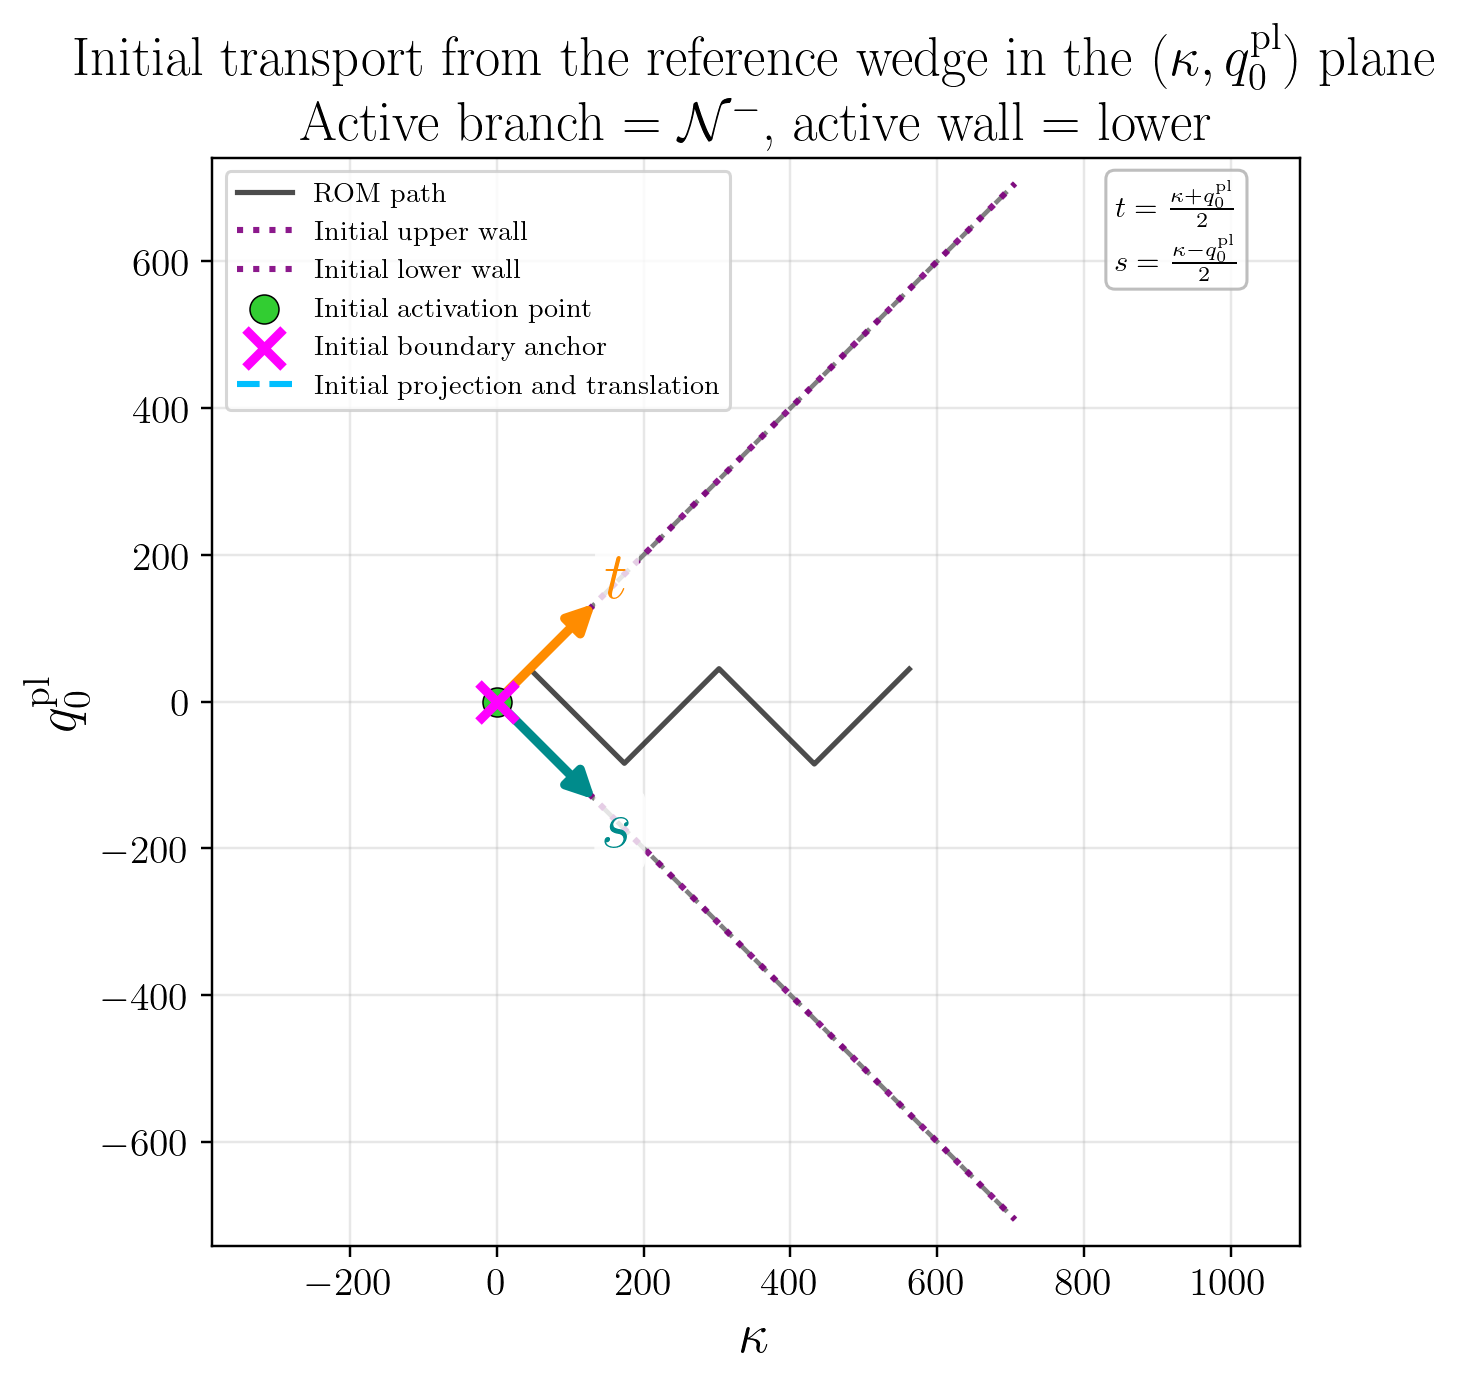
\includegraphics[width=0.74\textwidth]{two_surface_switch_with_boundary_projection_transport/initial_wedge_xy.png}
\caption{Reference wedge in the \((\kappa,q^{\mathrm{pl}}_0)\) plane and initial active point of the ROM trajectory. The arrows indicate the \(t\)- and \(s\)-directions associated with the equivalent quadrant coordinates.}
\label{fig:transport_initial_xy_ts_ref}
\end{figure}

\begin{figure}[H]
\centering
\begin{subfigure}{0.32\textwidth}
\centering
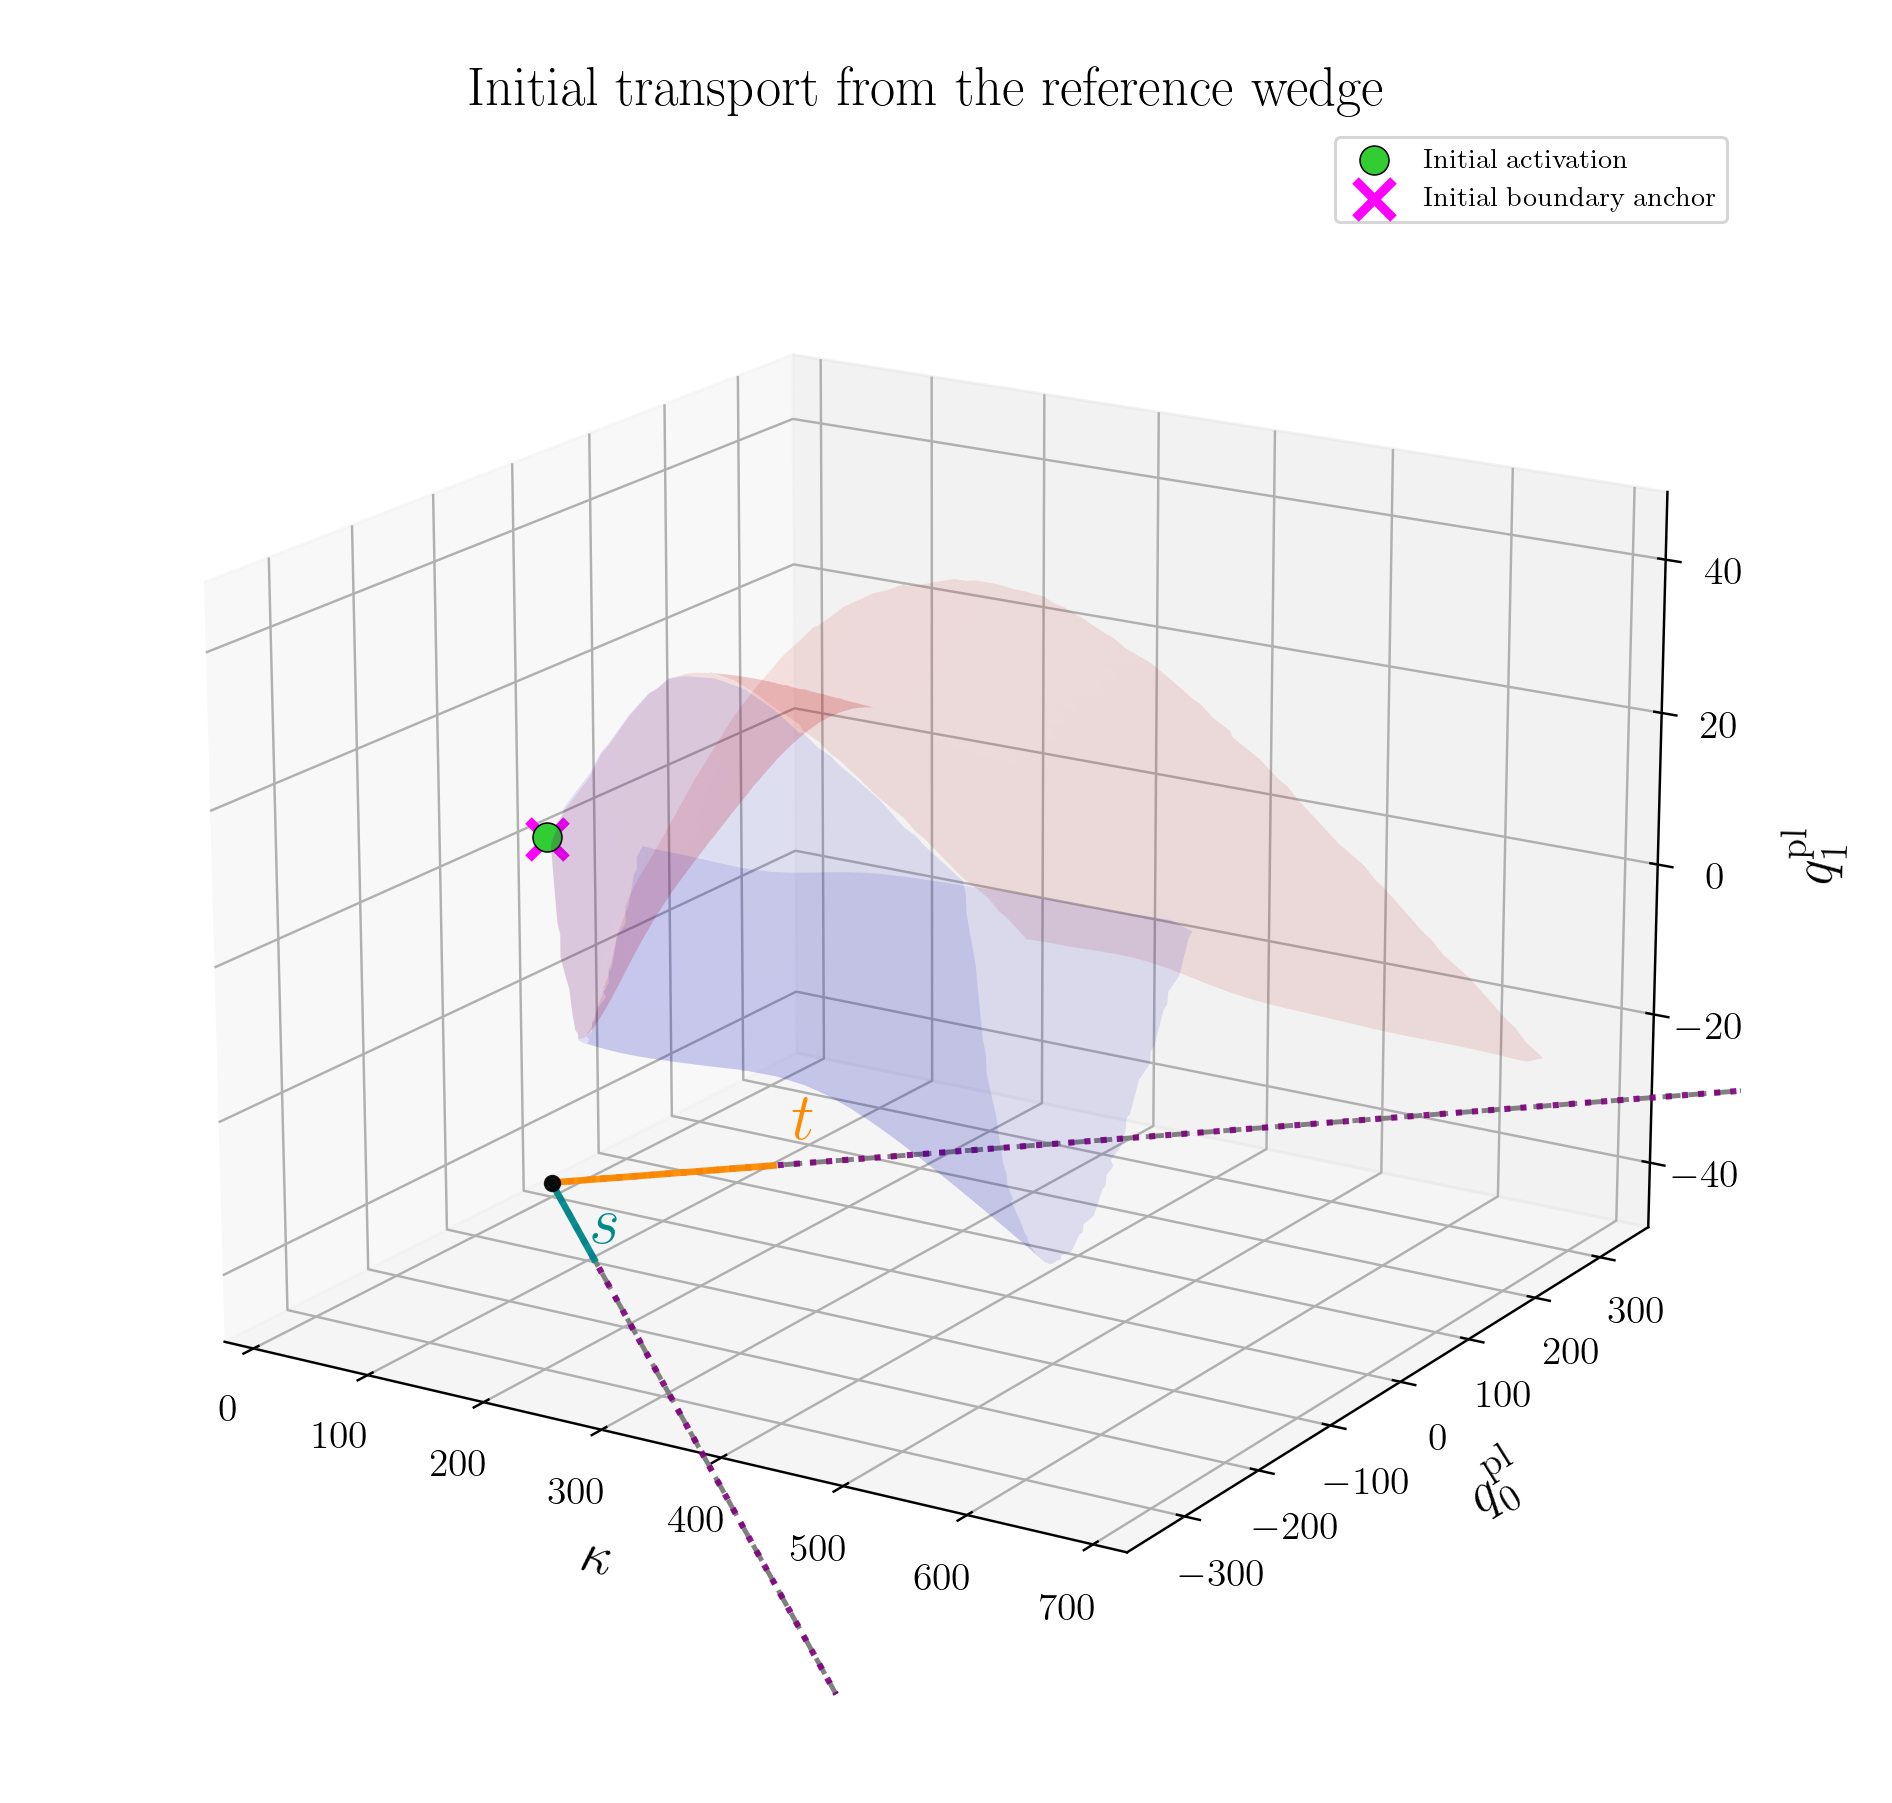
\includegraphics[width=\textwidth]{two_surface_switch_with_boundary_projection_transport/initial_transport_view1.png}
\caption{View 1}
\label{fig:init_transport_views_all_ts_ref_a}
\end{subfigure}
\hfill
\begin{subfigure}{0.32\textwidth}
\centering
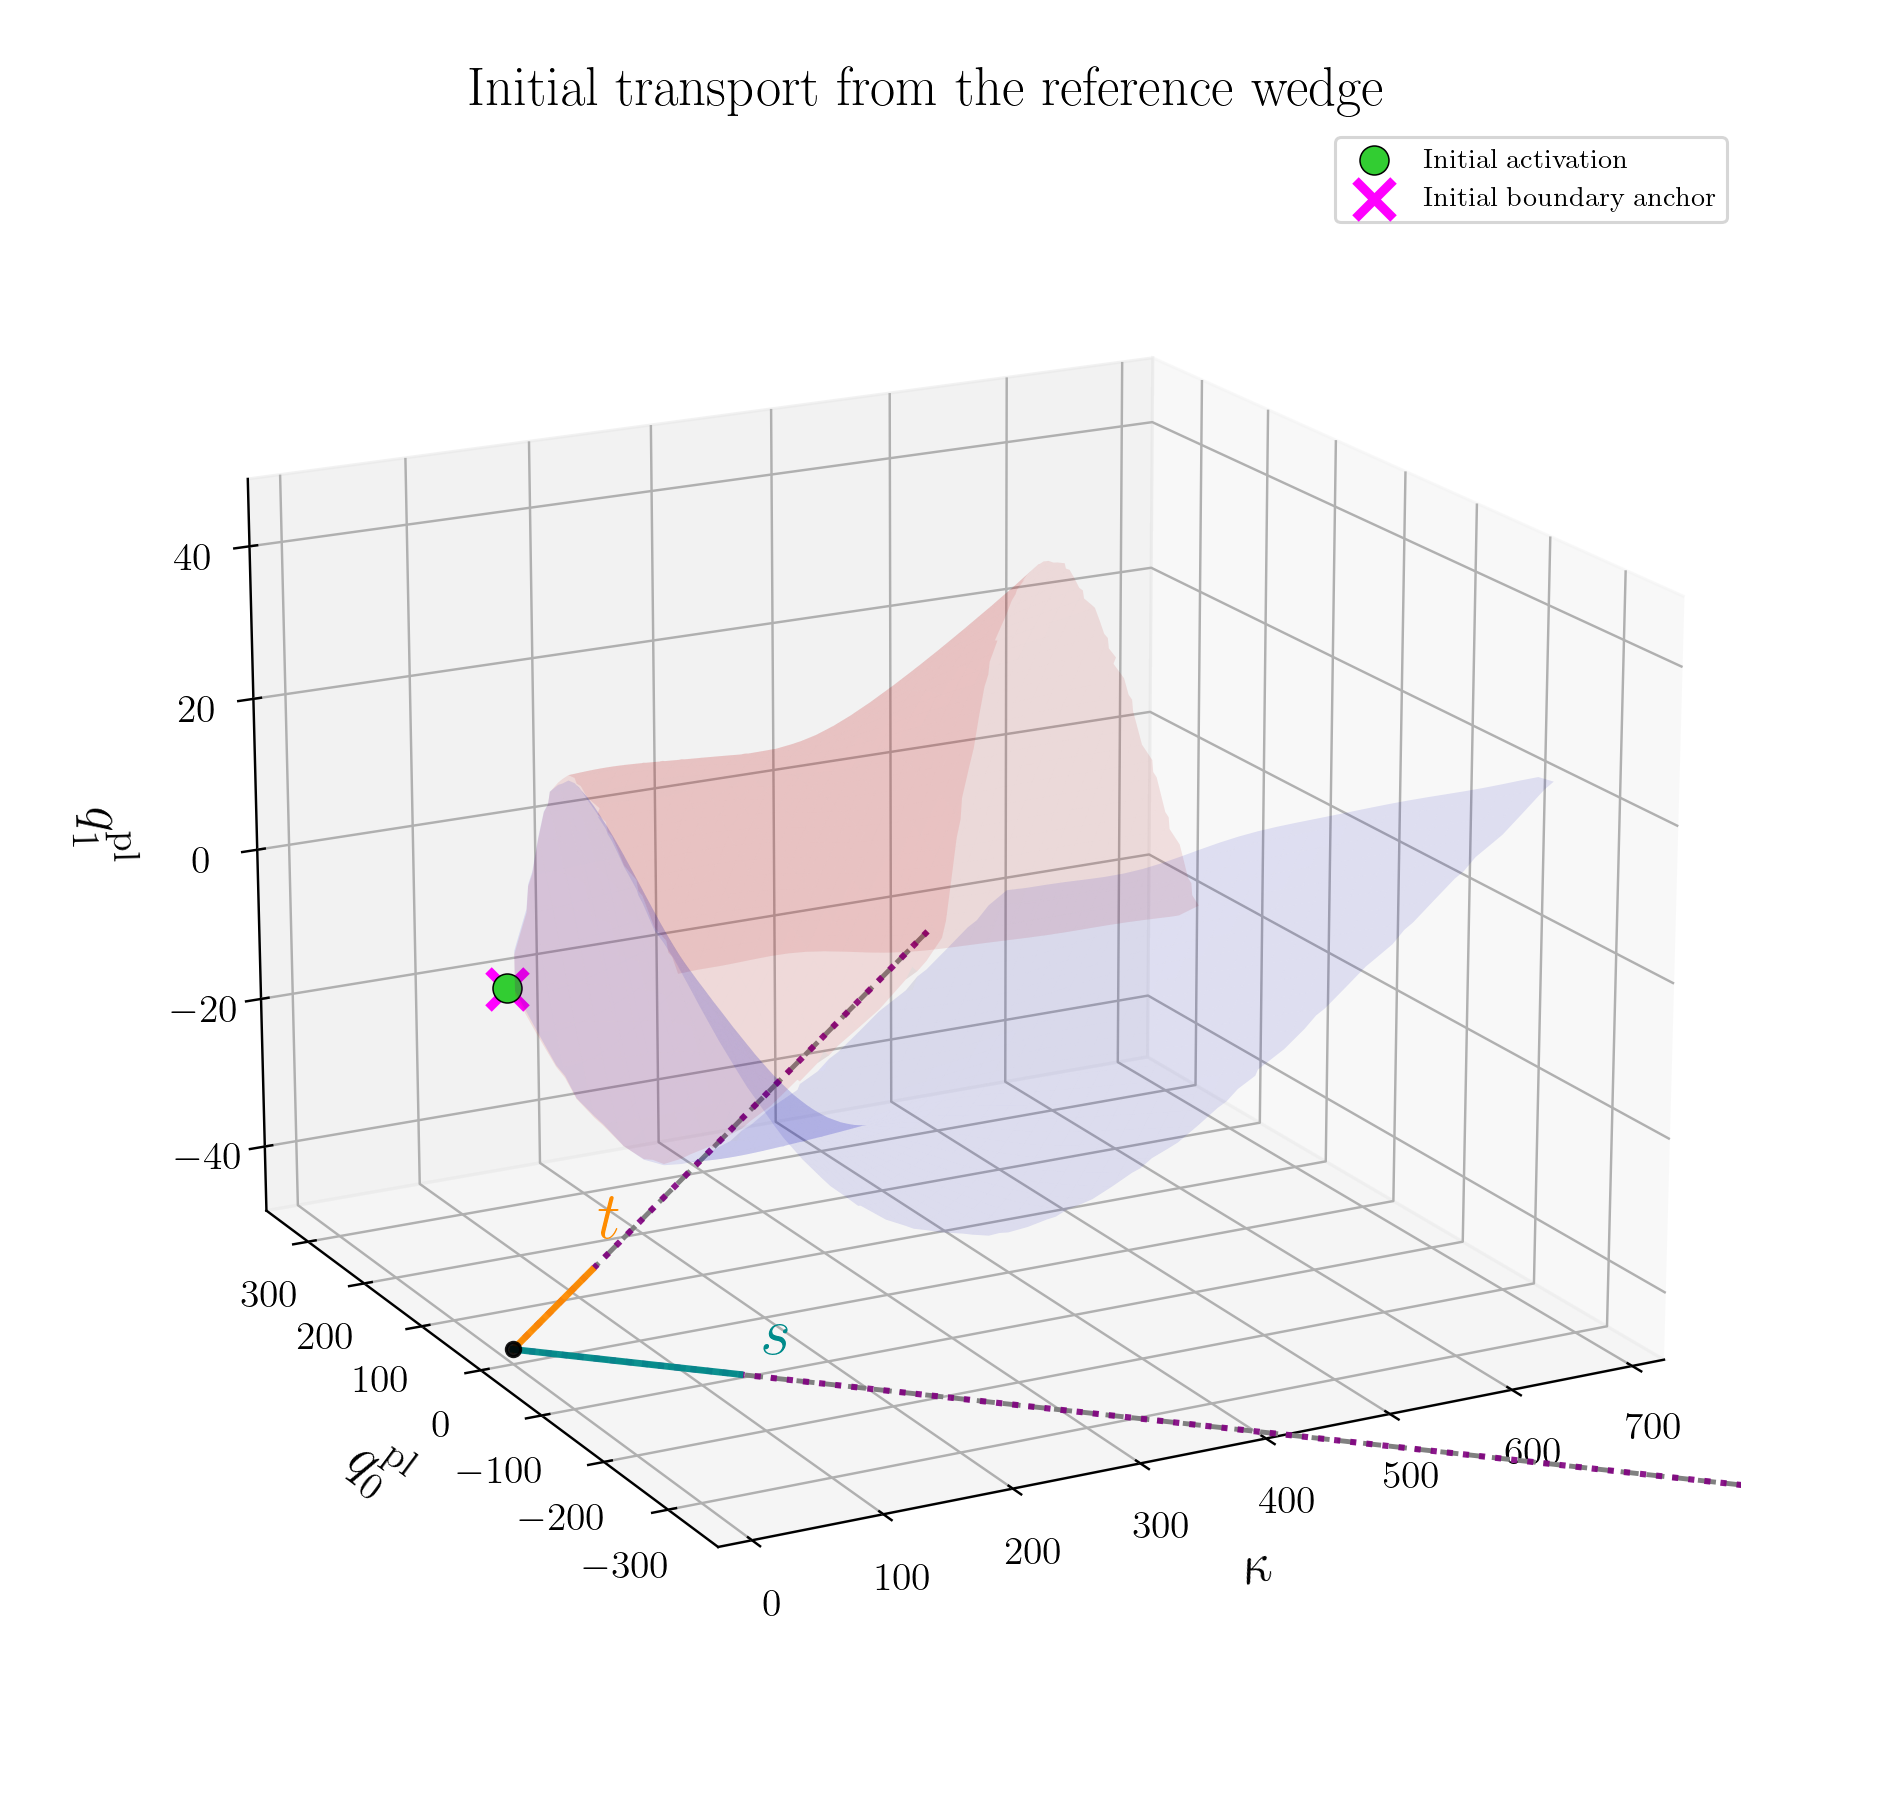
\includegraphics[width=\textwidth]{two_surface_switch_with_boundary_projection_transport/initial_transport_view2.png}
\caption{View 2}
\label{fig:init_transport_views_all_ts_ref_b}
\end{subfigure}
\hfill
\begin{subfigure}{0.32\textwidth}
\centering
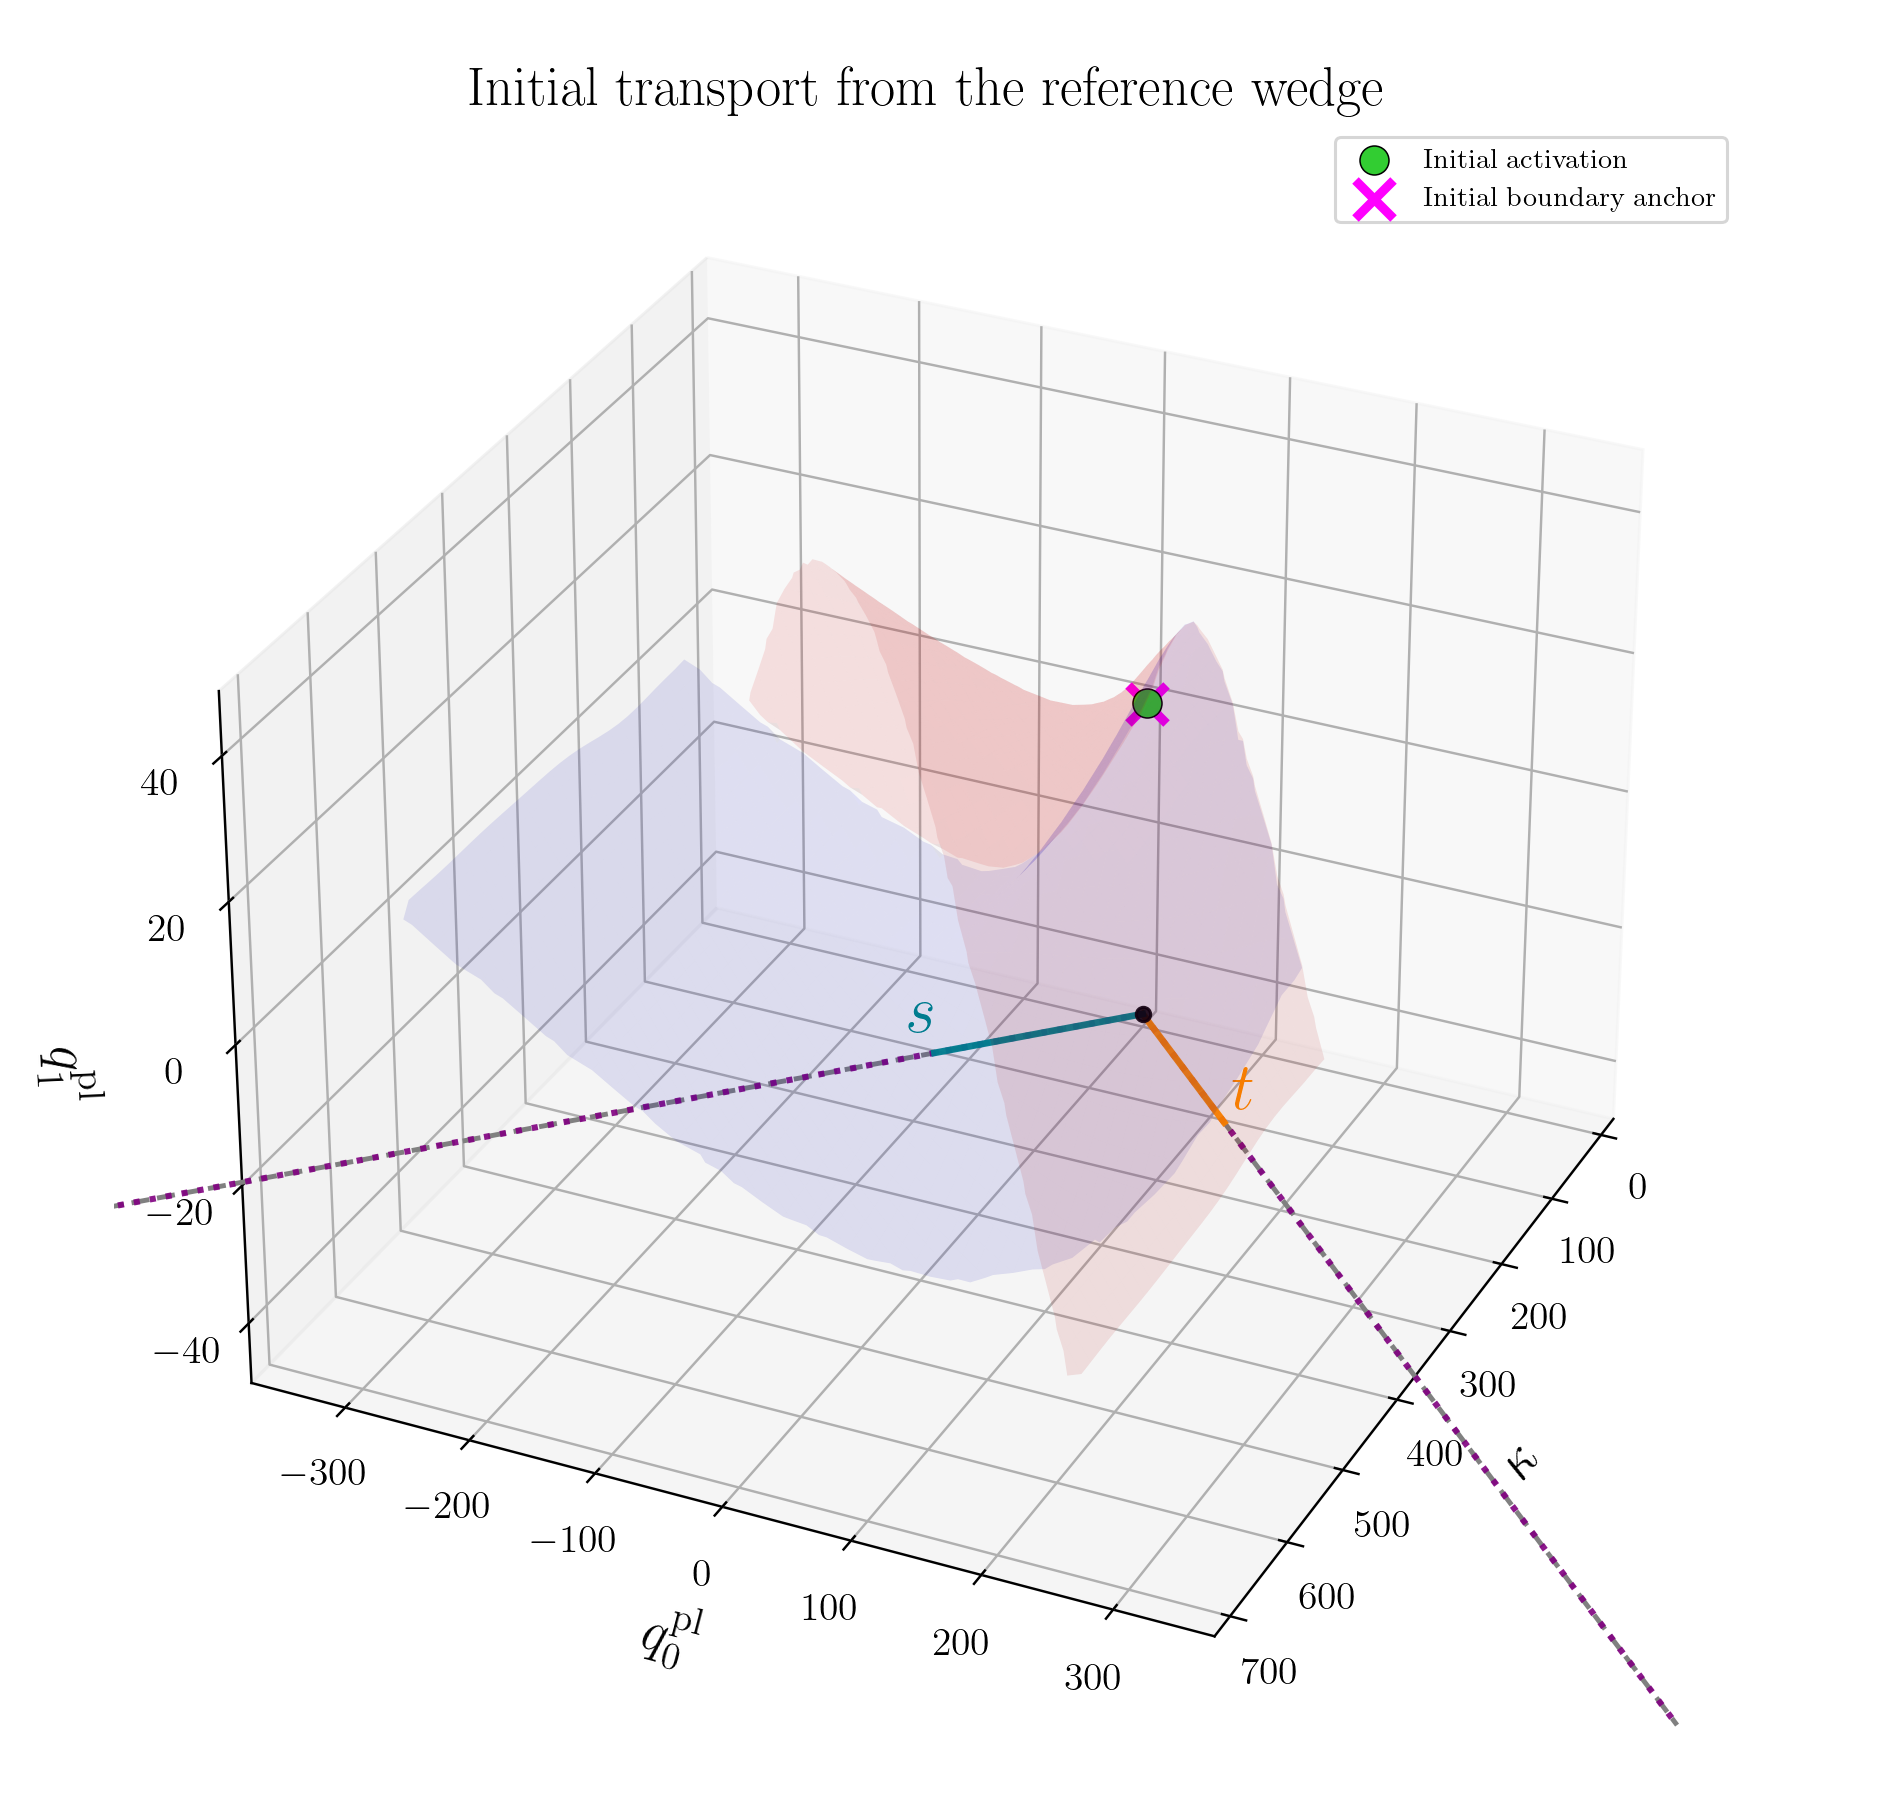
\includegraphics[width=\textwidth]{two_surface_switch_with_boundary_projection_transport/initial_transport_view3.png}
\caption{View 3}
\label{fig:init_transport_views_all_ts_ref_c}
\end{subfigure}
\caption{Initial anchoring of the first active branch in the latent space \((\kappa,q^{\mathrm{pl}}_0,q^{\mathrm{pl}}_1)\). The displayed vertical coordinate is \(q^{\mathrm{pl}}_1\), while the construction itself is intended for the full target vector \(\mathbf{q}^{\mathrm{pl}}_{\mathrm{tgt}}\).}
\label{fig:init_transport_views_all_ts_ref}
\end{figure}

\subsection{Prediction inside one branch segment}

Assume that over a certain interval the active branch remains fixed, and denote it by \(\beta_n\in\{-,+\}\). Then the transported prediction of the target vector is
\begin{equation}
\widehat{\mathbf{q}}^{\mathrm{pl}}_{\mathrm{tgt},n}
=
\widetilde{\mathcal{N}}^{\beta_n}(\kappa_n,q^{\mathrm{pl}}_{0,n}).
\label{eq:prediction_segment_vector_transport_ref}
\end{equation}
Equivalently,
\begin{equation}
\widehat{\mathbf{q}}^{\mathrm{pl}}_{\mathrm{tgt},n}
=
\widetilde{\widehat{\mathcal{N}}}^{\beta_n}(t_n,s_n).
\label{eq:prediction_segment_ts_transport_ref}
\end{equation}

Expanding the transported map gives
\begin{equation}
\widehat{\mathbf{q}}^{\mathrm{pl}}_{\mathrm{tgt},n}
=
\mathcal{N}^{\beta_n}
\!\left(
\kappa_n-\Delta K,\;
q^{\mathrm{pl}}_{0,n}-\Delta Q_0
\right)
+
\Delta \mathbf{Q}_{\mathrm{tgt}}^{\beta_n},
\label{eq:prediction_segment_explicit_transport_ref}
\end{equation}
or, in \((t,s)\) coordinates,
\begin{equation}
\widehat{\mathbf{q}}^{\mathrm{pl}}_{\mathrm{tgt},n}
=
\widehat{\mathcal{N}}^{\beta_n}
\!\left(
t_n-\Delta t,\;
s_n-\Delta s
\right)
+
\Delta \mathbf{Q}_{\mathrm{tgt}}^{\beta_n}.
\label{eq:prediction_segment_explicit_ts_transport_ref}
\end{equation}

Hence, while the branch remains unchanged, the transport state is frozen and the current point is simply evaluated on the currently transported active branch.

Figure~\ref{fig:transport_stageB_q1_ts_ref} compares the transported prediction with the ROM history of \(q^{\mathrm{pl}}_1\). The close agreement confirms that, once the transport state is updated appropriately, the branchwise latent surrogate tracks the ROM target coordinate accurately along the whole trajectory.

\begin{figure}[H]
\centering
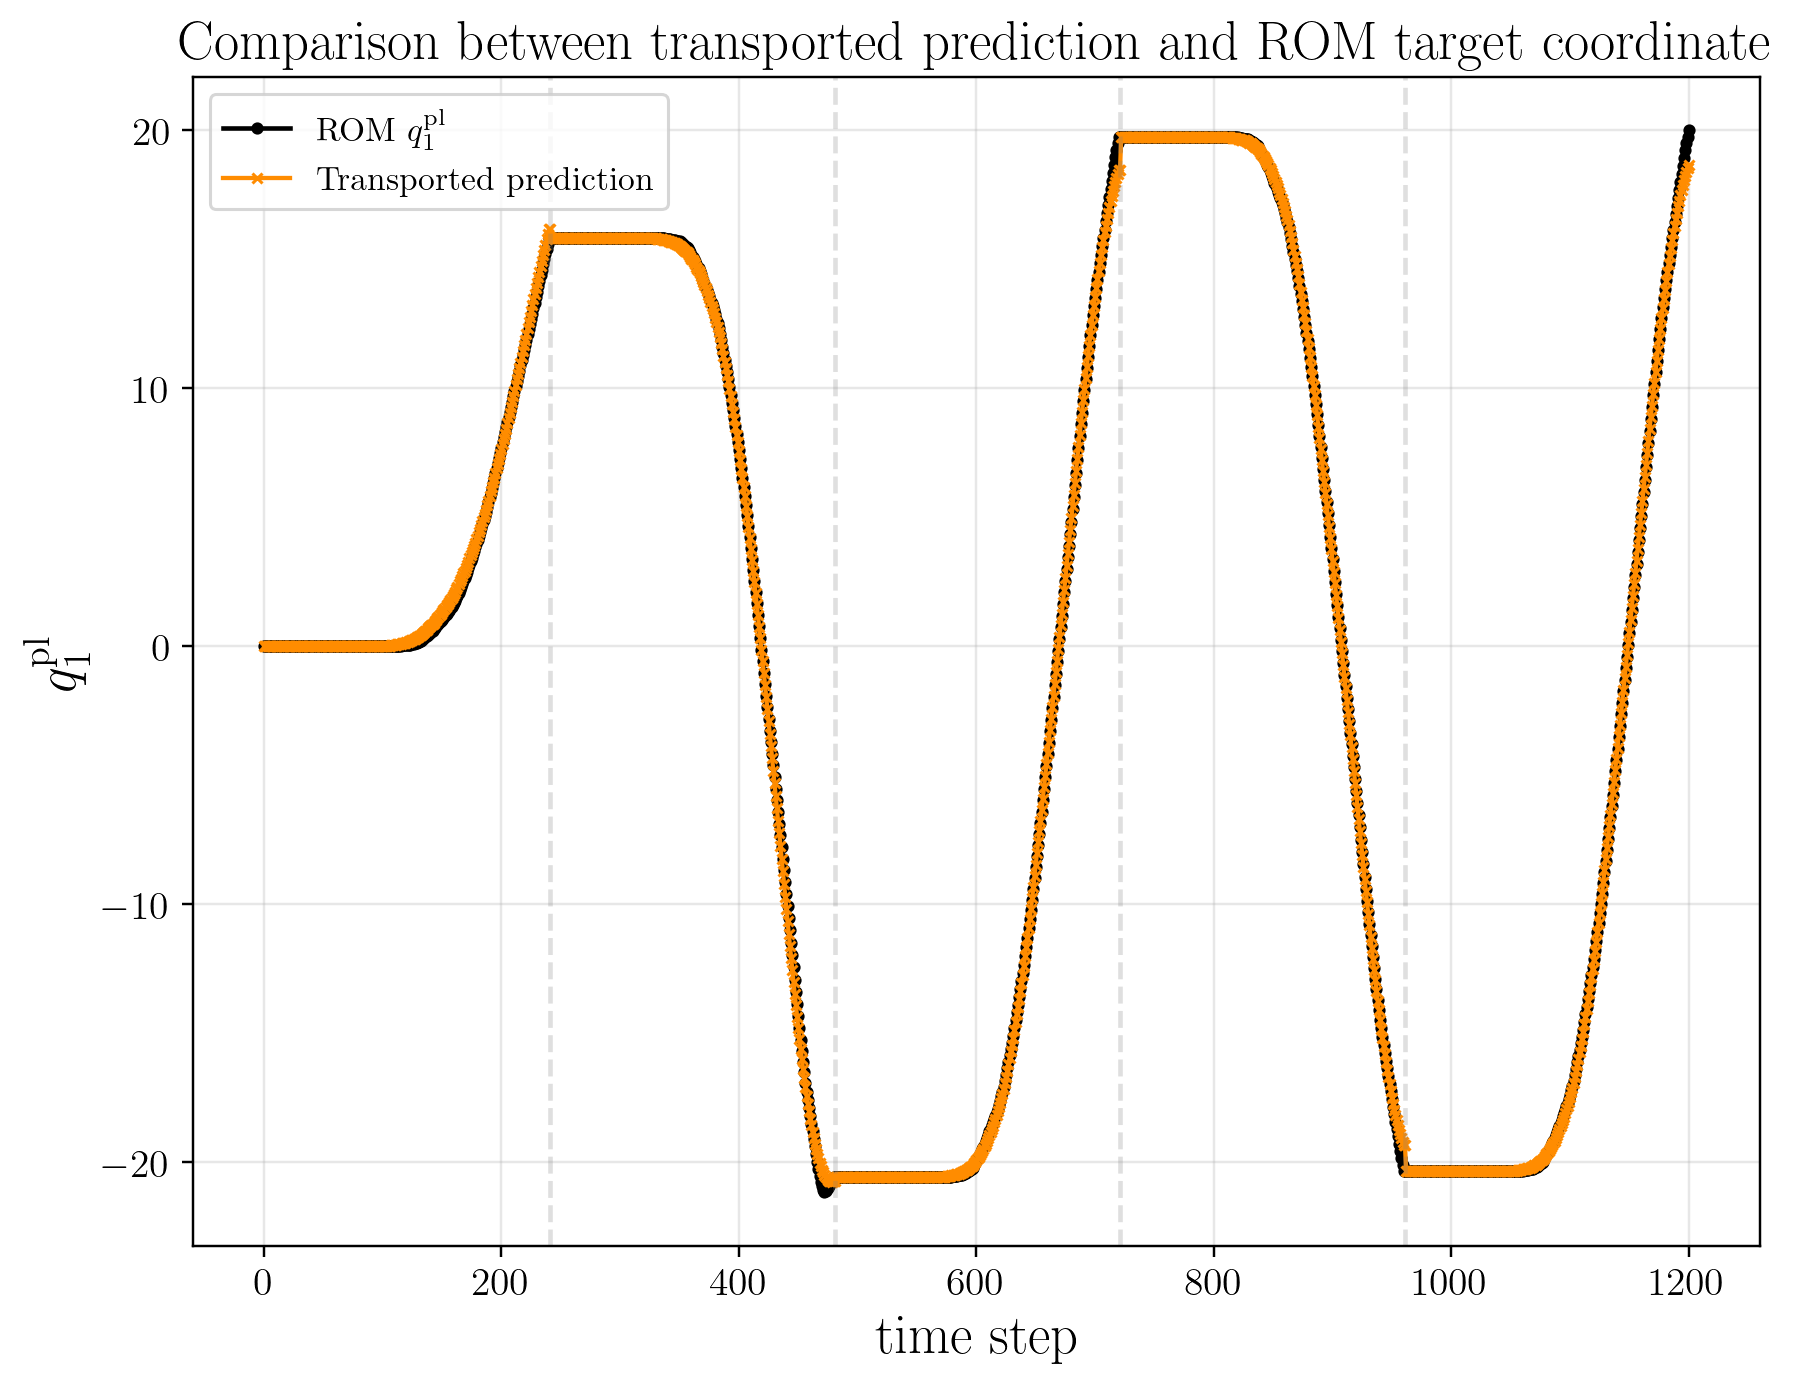
\includegraphics[width=0.74\textwidth]{two_surface_switch_with_boundary_projection_transport/stageB_qpl1_vs_step.png}
\caption{Comparison between the transported prediction and the ROM history of \(q^{\mathrm{pl}}_1\). Vertical dashed lines indicate switching instants.}
\label{fig:transport_stageB_q1_ts_ref}
\end{figure}

\subsection{Switch update}

Suppose that at step \(n_c\) the sign of \(\Delta \varepsilon_{xx}^{M}\) changes. Let
\[
P_c=(\kappa_c,q^{\mathrm{pl}}_{0,c})
\]
be the switching point in the latent plane, and let
\[
\mathbf{q}^{\mathrm{pl}}_{\mathrm{tgt},c}
\]
denote the corresponding ROM target vector. Let \(\beta_{\mathrm{new}}\in\{-,+\}\) denote the newly active branch.

The switch update consists of four steps.

\paragraph{Step 1. Projection onto the transported boundary.}
Project \(P_c\) onto the transported upper or lower wall associated with the new branch. In the \((\kappa,q^{\mathrm{pl}}_0)\) frame this is given by \eqref{eq:projection_upper_transport_ref} or \eqref{eq:projection_lower_transport_ref}. In the \((t,s)\) frame the same operation is projection onto one transported axis:
\[
(t_c,s_c)\mapsto (t_c,\Delta s)
\quad\text{or}\quad
(t_c,s_c)\mapsto (\Delta t,s_c).
\]
This produces the boundary anchor \(P_b\).

\paragraph{Step 2. Evaluation of the newly active transported branch at the anchor.}
Compute
\begin{equation}
\mathbf{q}^{\mathrm{pl}}_{\mathrm{tgt},b}
=
\widetilde{\mathcal{N}}^{\beta_{\mathrm{new}}}
(\kappa_b,q^{\mathrm{pl}}_{0,b}),
\label{eq:q_target_boundary_anchor_transport_ref}
\end{equation}
or equivalently
\begin{equation}
\mathbf{q}^{\mathrm{pl}}_{\mathrm{tgt},b}
=
\widetilde{\widehat{\mathcal{N}}}^{\beta_{\mathrm{new}}}
(t_b,s_b).
\label{eq:q_target_boundary_anchor_ts_transport_ref}
\end{equation}

\paragraph{Step 3. In-plane translation.}
Update the shared in-plane transport so that the boundary anchor reaches the switch point:
\begin{align}
\Delta K &\leftarrow \Delta K + (\kappa_c-\kappa_b),
\label{eq:update_deltaK_transport_ref}
\\
\Delta Q_0 &\leftarrow \Delta Q_0 + (q^{\mathrm{pl}}_{0,c}-q^{\mathrm{pl}}_{0,b}).
\label{eq:update_deltaQ0_transport_ref}
\end{align}
Equivalently,
\begin{align}
\Delta t &\leftarrow \Delta t + (t_c-t_b),
\label{eq:update_deltat_transport_ref}
\\
\Delta s &\leftarrow \Delta s + (s_c-s_b).
\label{eq:update_deltas_transport_ref}
\end{align}

\paragraph{Step 4. Vertical re-anchoring of the newly active branch.}
Update the branch-specific target offset by
\begin{equation}
\Delta \mathbf{Q}_{\mathrm{tgt}}^{\beta_{\mathrm{new}}}
\leftarrow
\Delta \mathbf{Q}_{\mathrm{tgt}}^{\beta_{\mathrm{new}}}
+
\left(
\mathbf{q}^{\mathrm{pl}}_{\mathrm{tgt},c}
-
\mathbf{q}^{\mathrm{pl}}_{\mathrm{tgt},b}
\right).
\label{eq:update_deltaQ_target_transport_ref}
\end{equation}

After this correction, the newly active transported surface passes exactly through the switch point.

\subsection{Interpretation of the switch mechanism}

The switch mechanism has a simple geometric interpretation. The current ROM point is not sent directly to the new offline branch. Instead, the new branch is first accessed through a boundary anchor on the current transported wedge. Then the full in-plane frame is translated so that this anchor coincides with the actual switch point. Finally, only the newly active branch is vertically corrected to match the ROM target value there.

Therefore, the update contains two distinct ingredients:
\begin{itemize}
\item a \emph{global in-plane transport} shared by both branches,
\item a \emph{branch-specific vertical re-anchoring} applied only to the active branch.
\end{itemize}

This is the central mechanism by which path dependence is encoded in the transported surrogate.

\subsection{Global transported prediction}

After all initialization and switch updates have been applied, the full transported path can be visualized in the latent space \((\kappa,q^{\mathrm{pl}}_0,q^{\mathrm{pl}}_1)\). Figures~\ref{fig:global_transport_views_all_ts_ref_a}--\ref{fig:global_transport_views_all_ts_ref_c} show the resulting construction from three viewpoints. The original branchwise surfaces \(\mathcal{N}^{-}\) and \(\mathcal{N}^{+}\) remain visible, while the red transported path follows the ROM reference path through successive branch changes.

\begin{figure}[H]
\centering
\begin{subfigure}{0.32\textwidth}
\centering
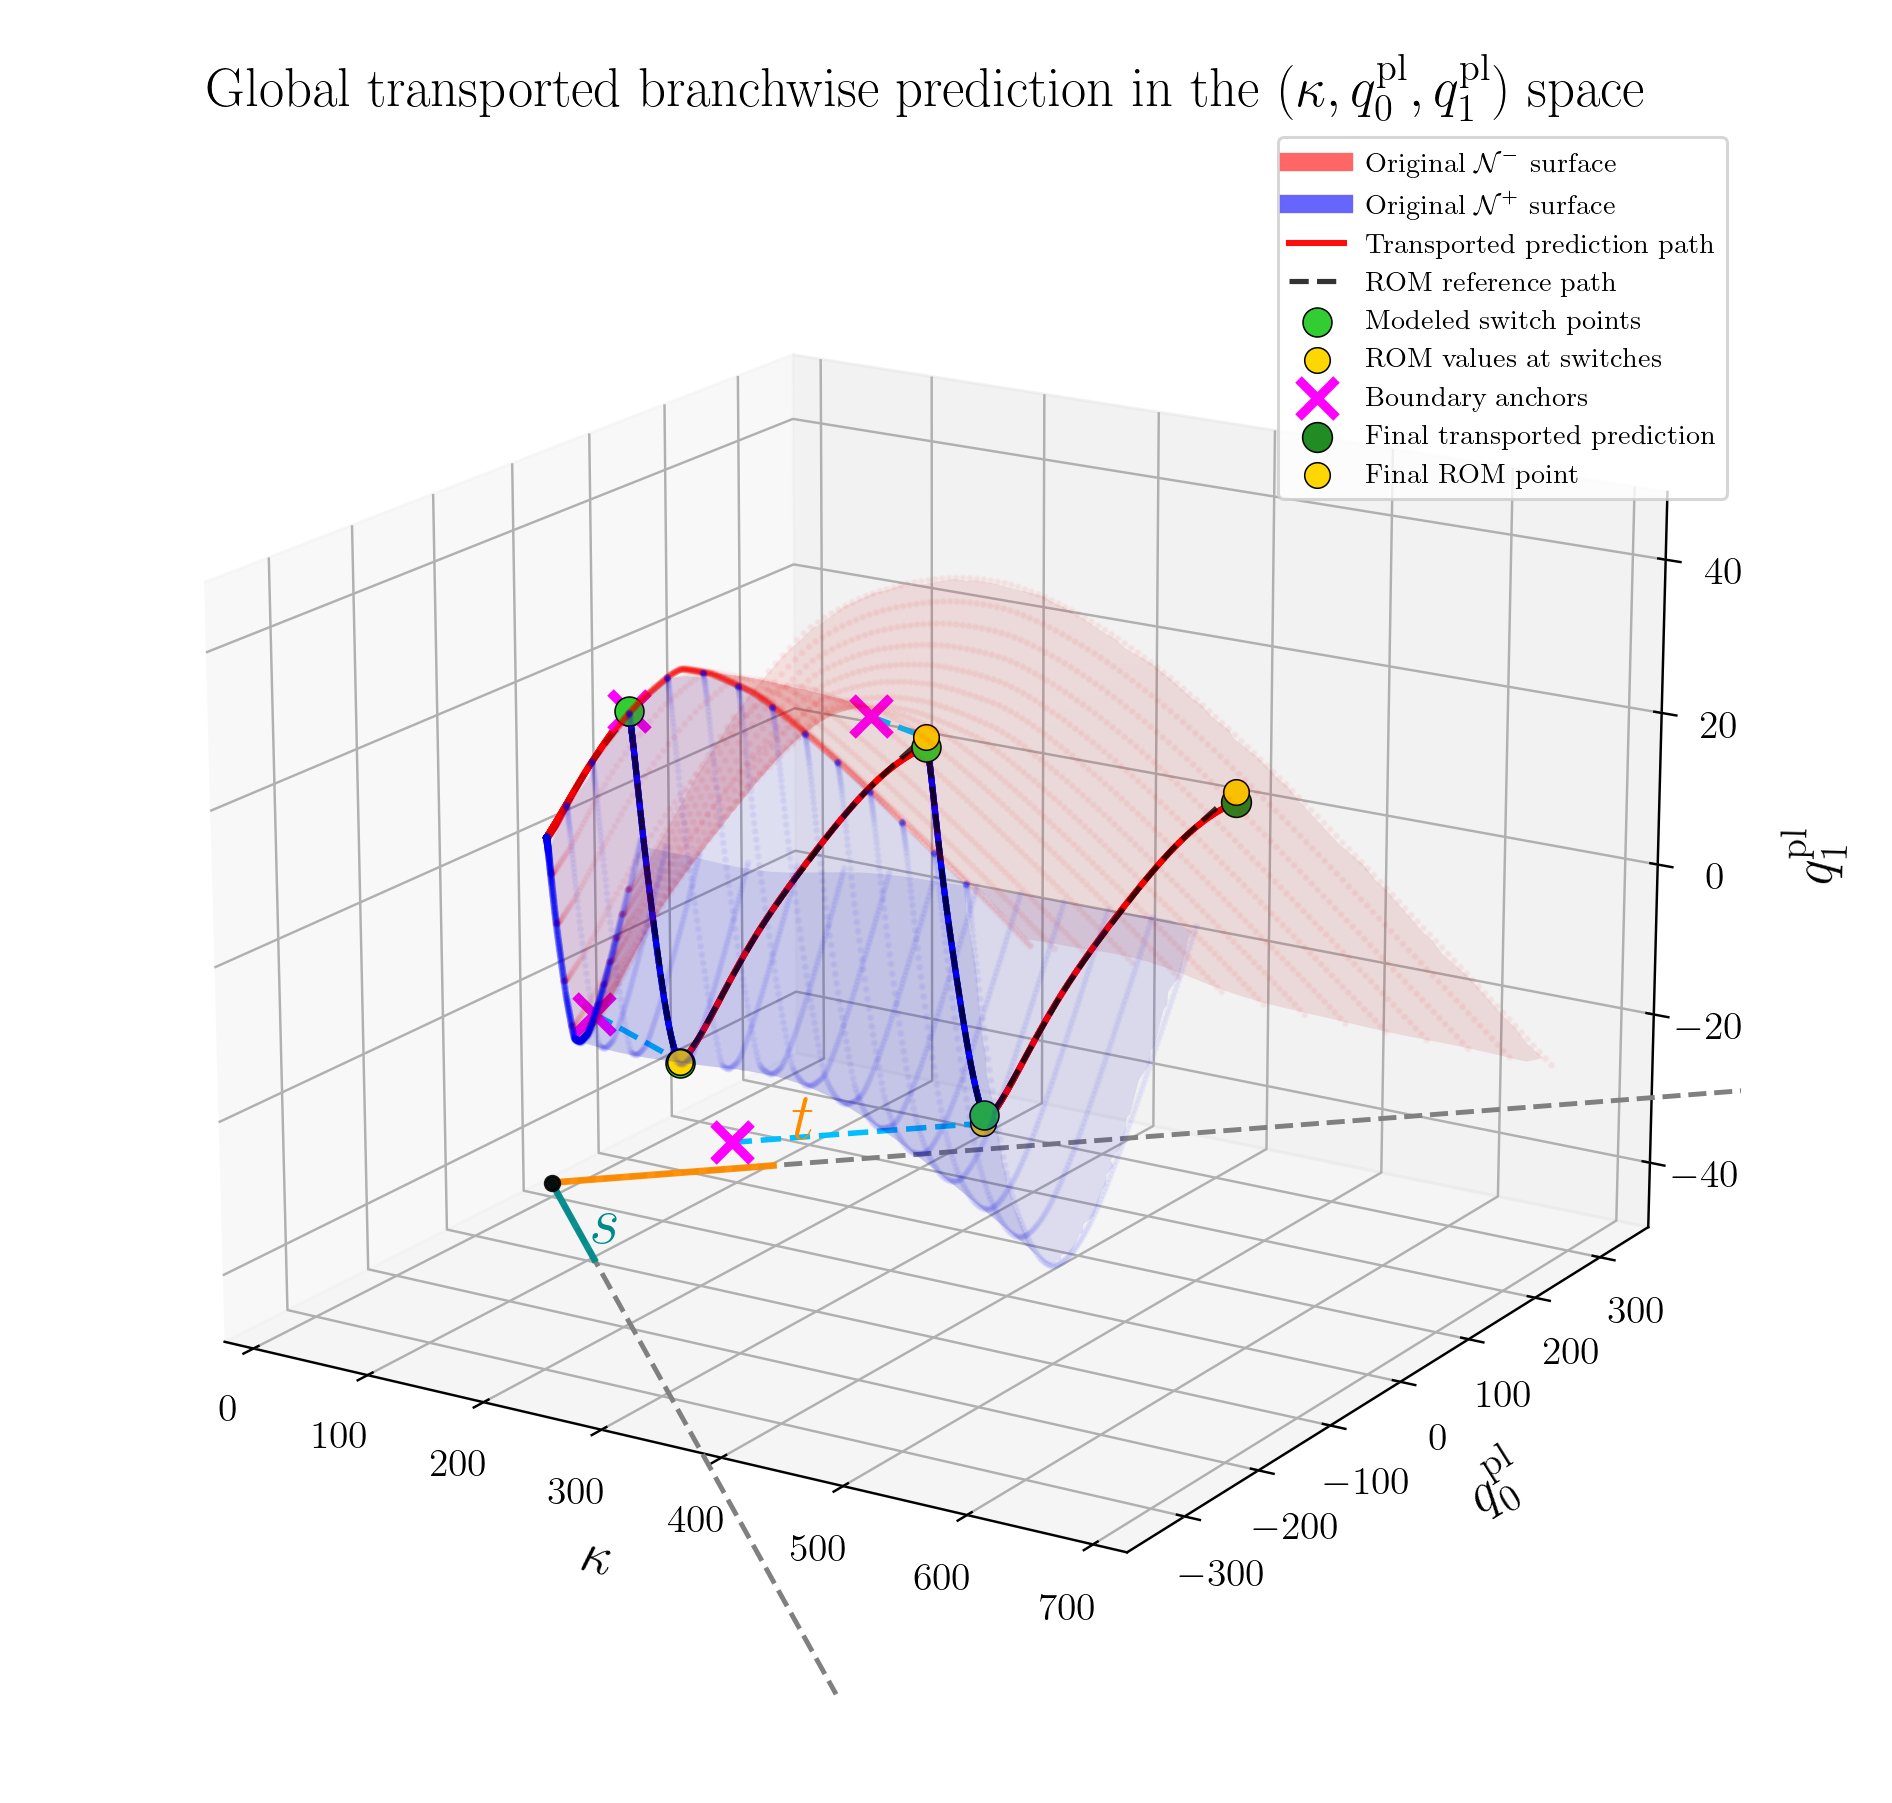
\includegraphics[width=\textwidth]{two_surface_switch_with_boundary_projection_transport/stageC_global_transport_view1.png}
\caption{View 1}
\label{fig:global_transport_views_all_ts_ref_a}
\end{subfigure}
\hfill
\begin{subfigure}{0.32\textwidth}
\centering
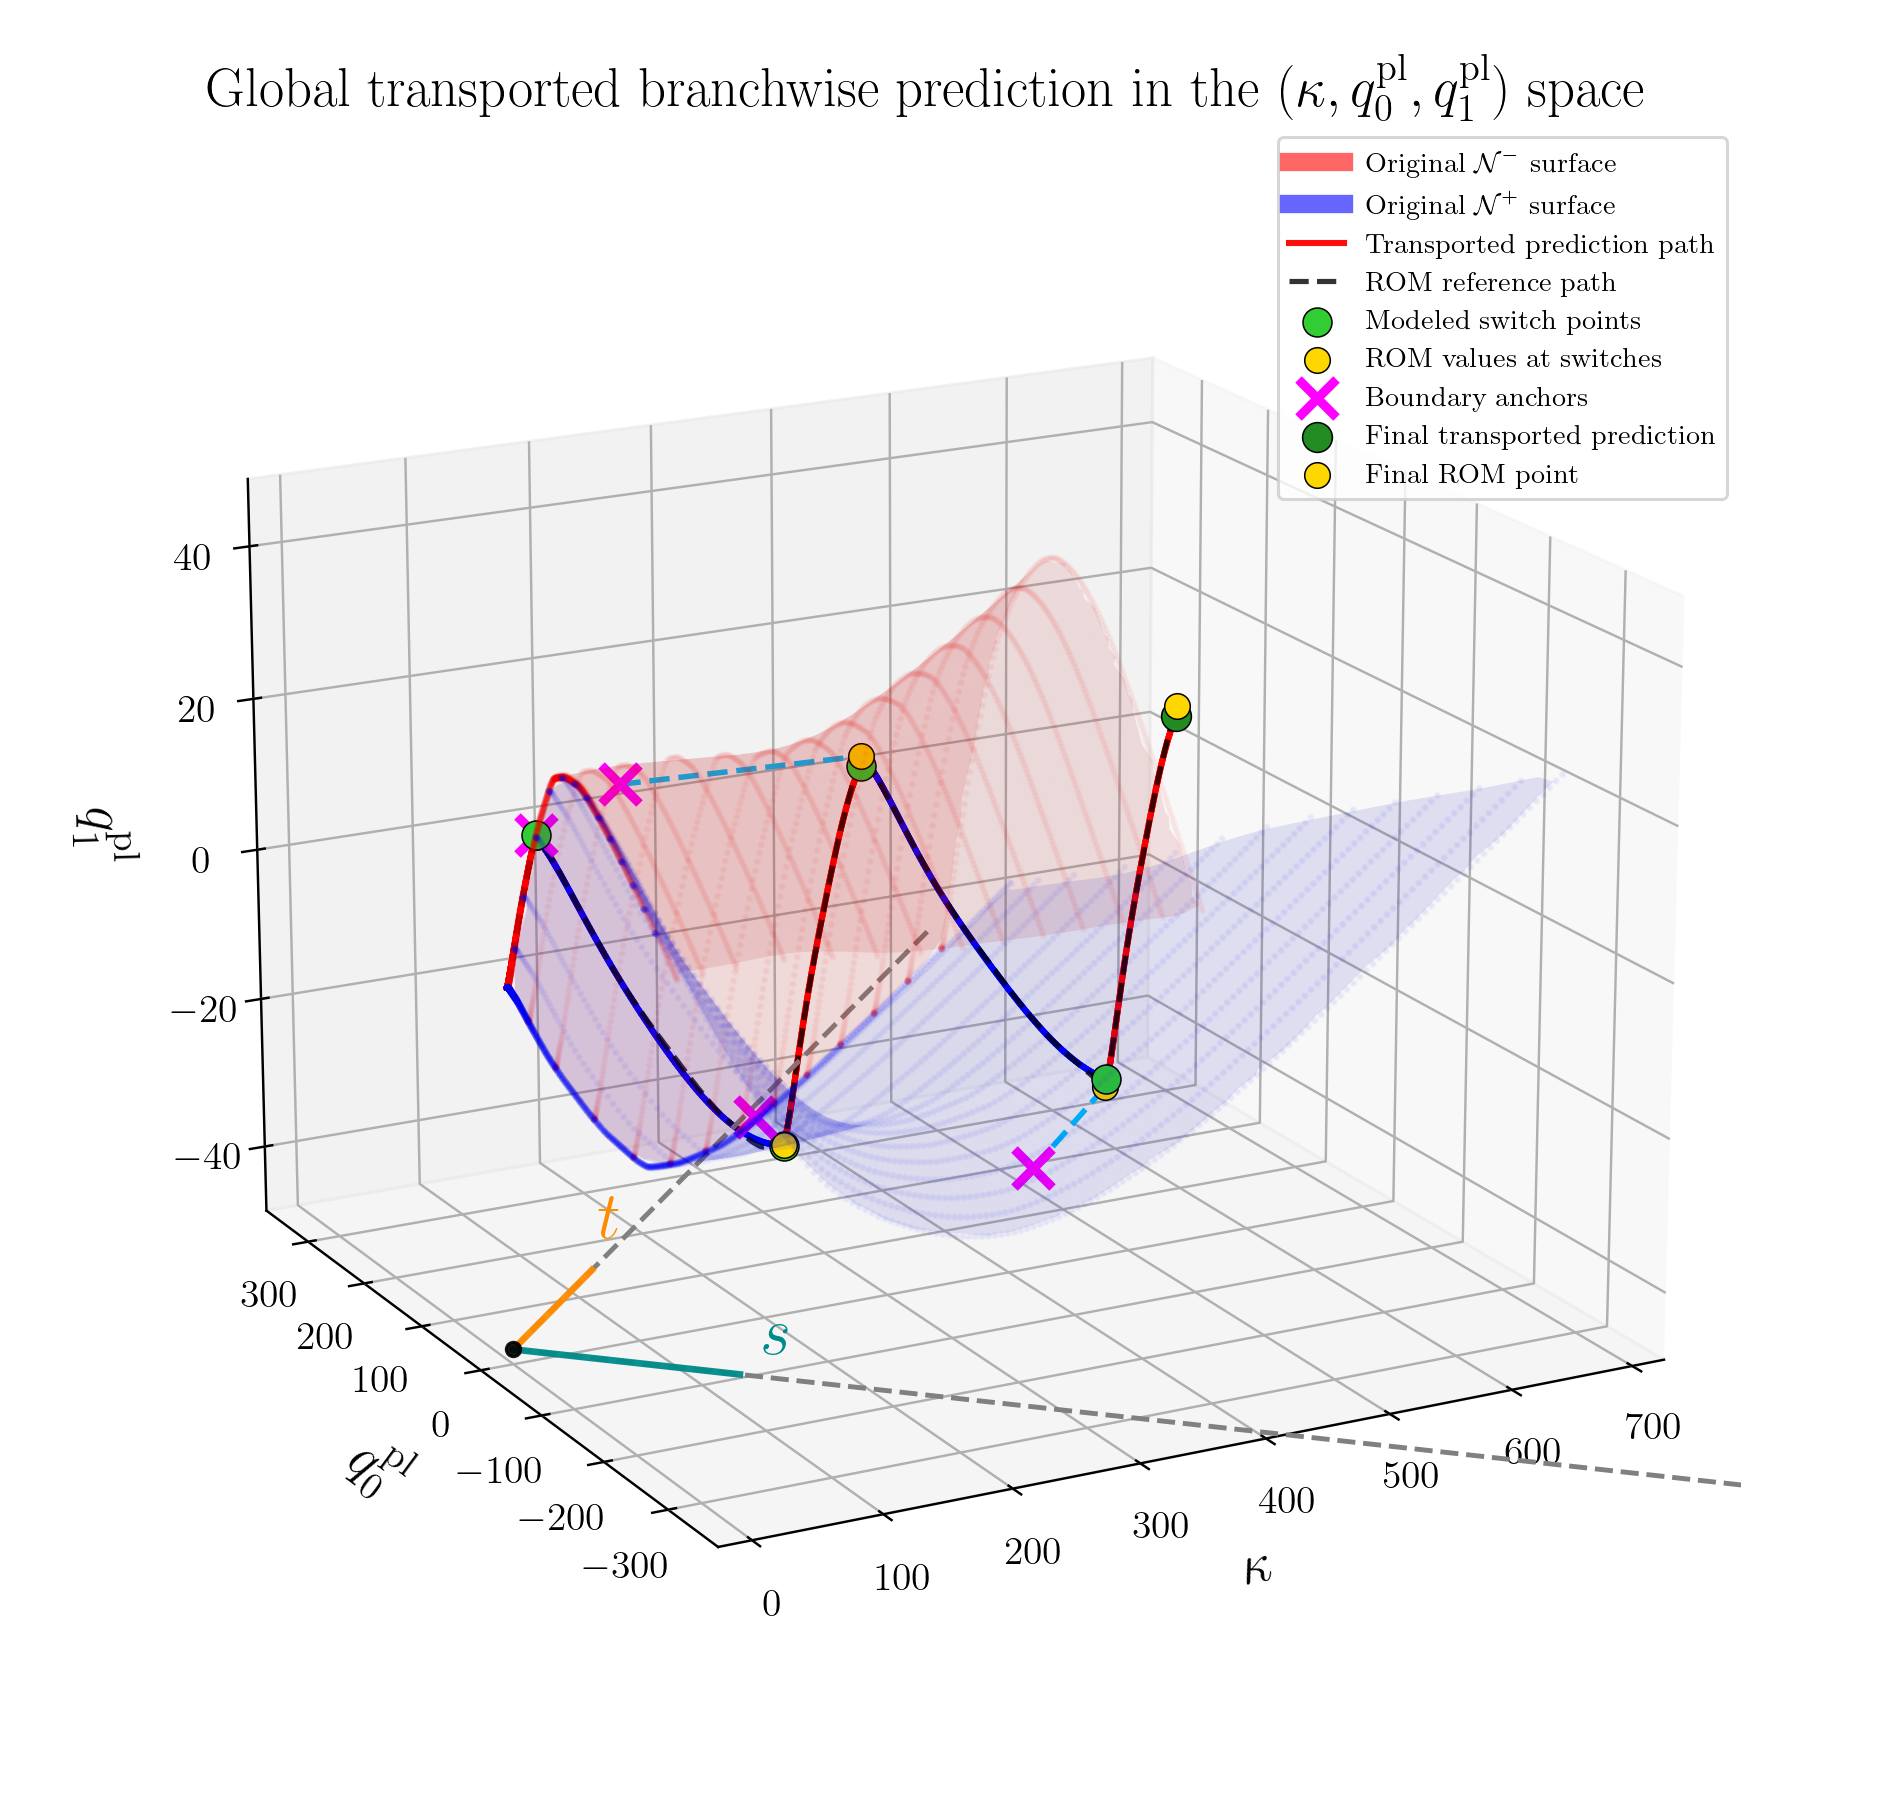
\includegraphics[width=\textwidth]{two_surface_switch_with_boundary_projection_transport/stageC_global_transport_view2.png}
\caption{View 2}
\label{fig:global_transport_views_all_ts_ref_b}
\end{subfigure}
\hfill
\begin{subfigure}{0.32\textwidth}
\centering
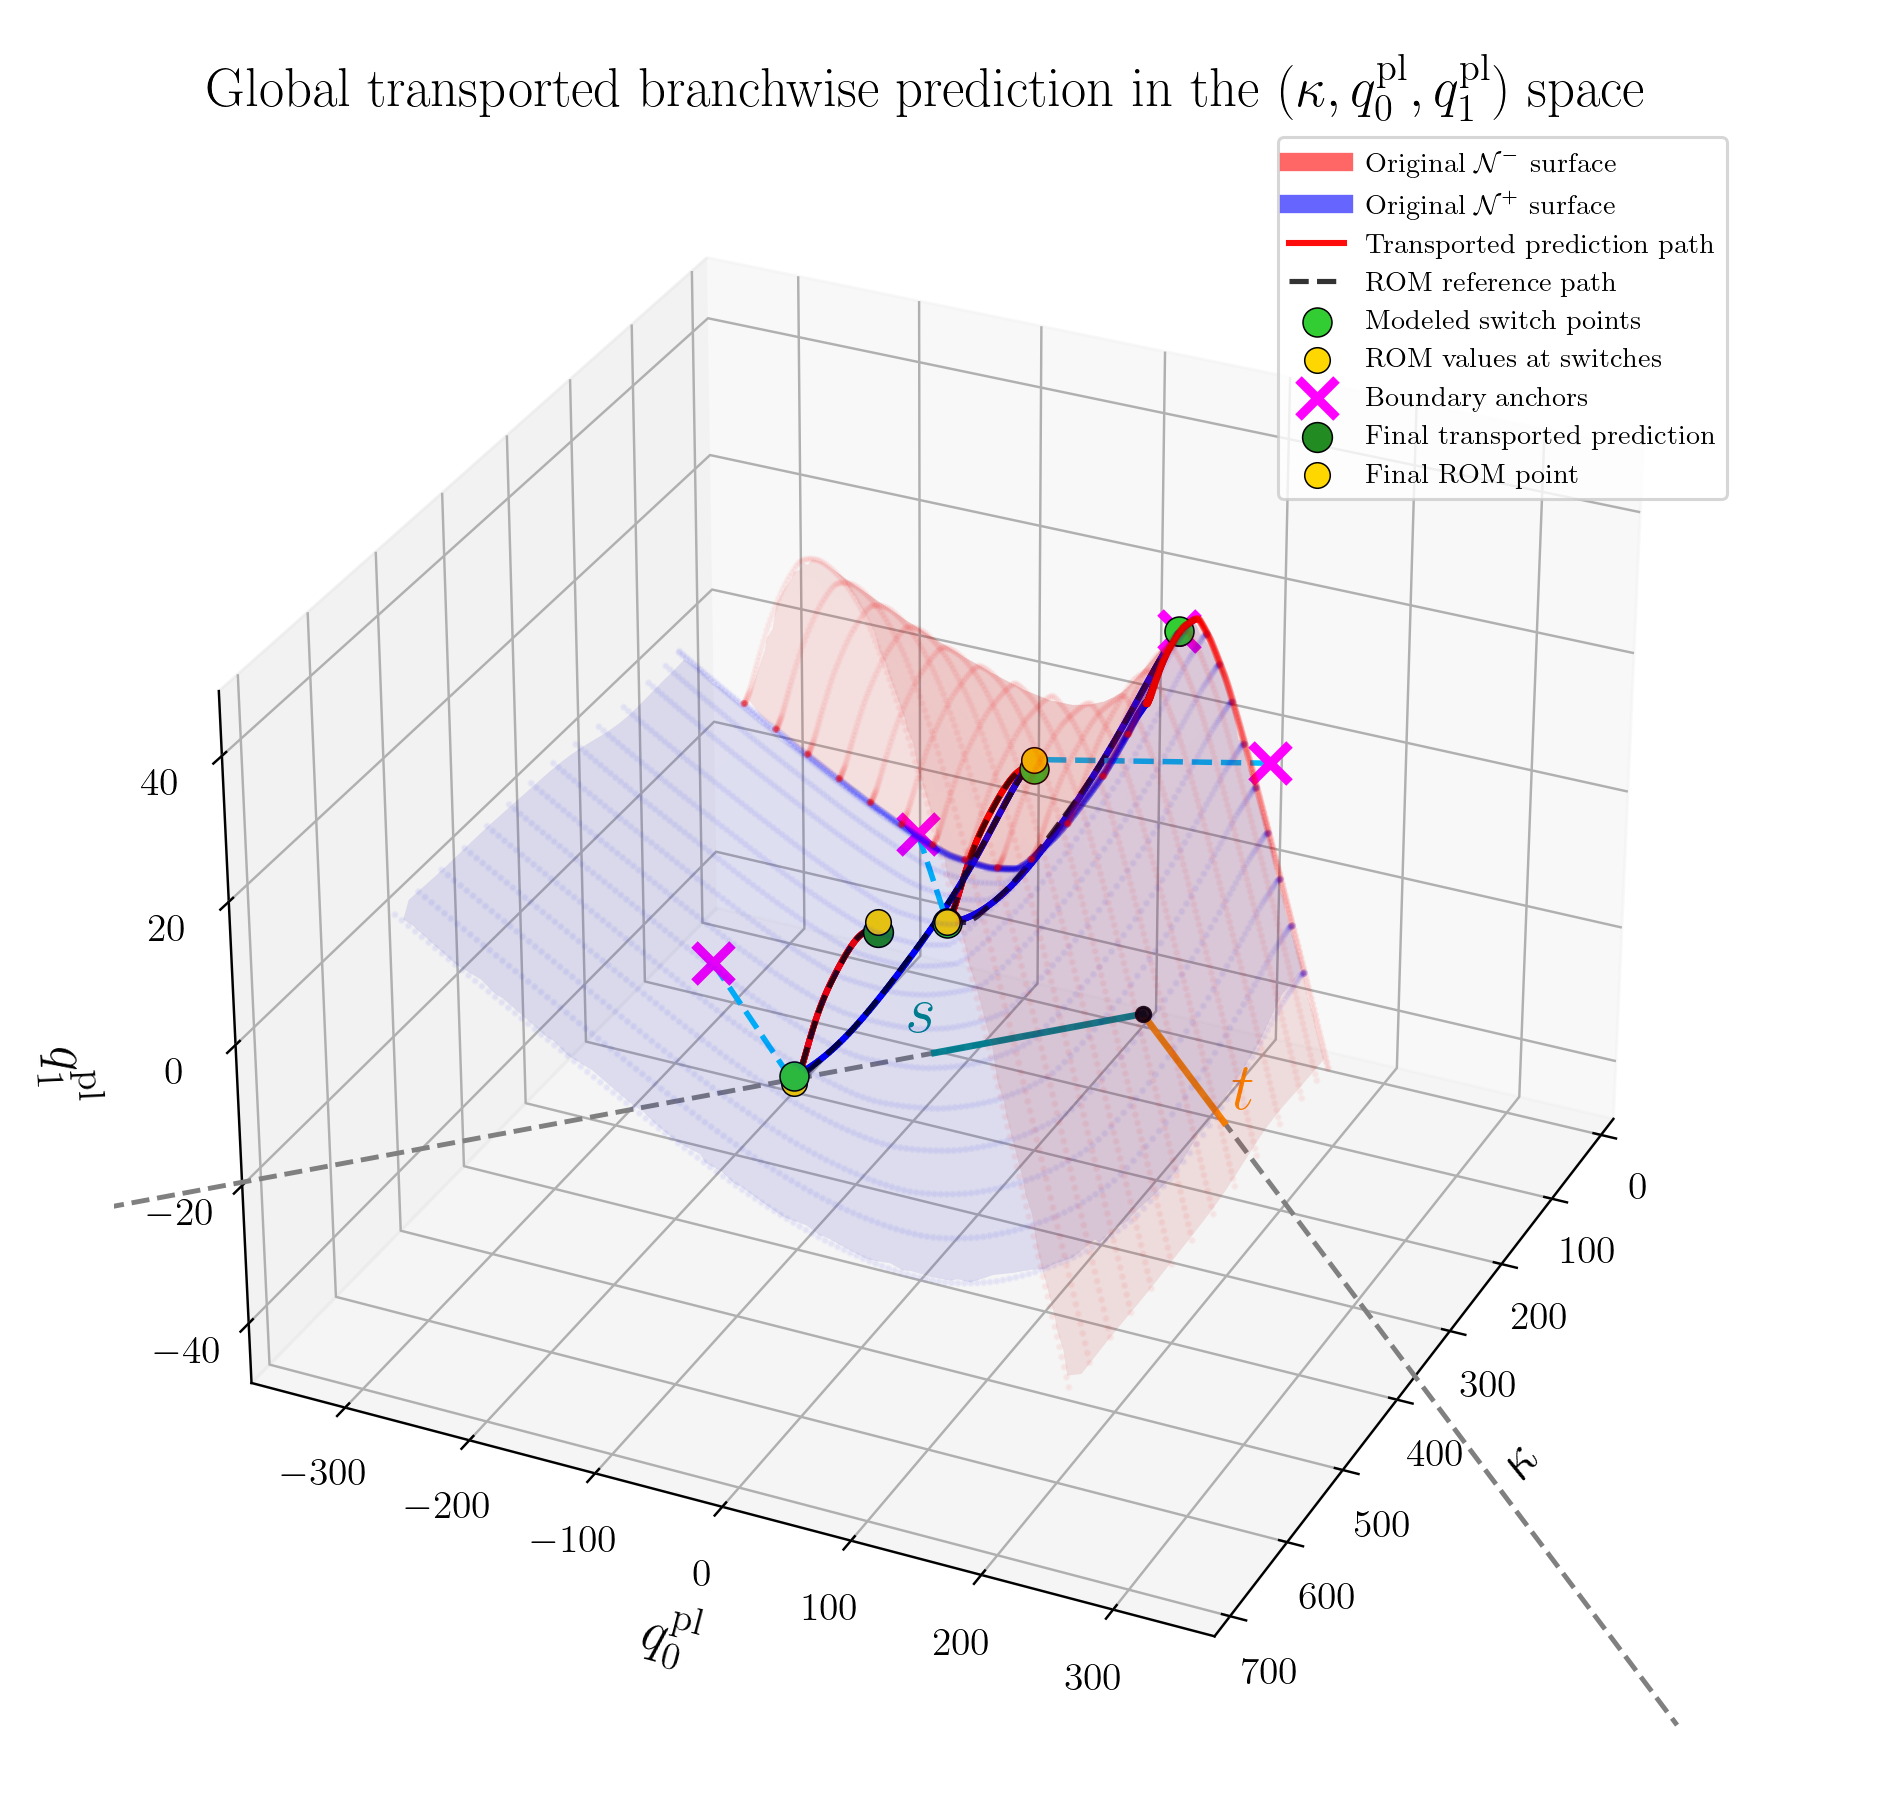
\includegraphics[width=\textwidth]{two_surface_switch_with_boundary_projection_transport/stageC_global_transport_view3.png}
\caption{View 3}
\label{fig:global_transport_views_all_ts_ref_c}
\end{subfigure}
\caption{Global transported branchwise prediction in the latent space. The red curve is the transported prediction, the dashed black curve is the ROM reference path, and the plotted vertical coordinate is \(q^{\mathrm{pl}}_1\).}
\label{fig:global_transport_views_all_ts_ref}
\end{figure}

The role of the transported construction may now be stated clearly. The two branchwise surfaces are fixed offline approximations of the latent target coordinates. The memory of the loading history is not represented by deforming these surfaces, but by updating the transport state
\begin{equation}
\Delta K,
\qquad
\Delta Q_0,
\qquad
\Delta \mathbf{Q}_{\mathrm{tgt}}^{-},
\qquad
\Delta \mathbf{Q}_{\mathrm{tgt}}^{+},
\label{eq:transport_state_final_transport_ref}
\end{equation}
or equivalently
\begin{equation}
\Delta t,
\qquad
\Delta s,
\qquad
\Delta \mathbf{Q}_{\mathrm{tgt}}^{-},
\qquad
\Delta \mathbf{Q}_{\mathrm{tgt}}^{+}.
\label{eq:transport_state_final_ts_transport_ref}
\end{equation}

In other words, the path dependence of the surrogate is encoded geometrically through cumulative translations of the latent frame together with branchwise vertical re-anchoring at switching events.

\section{Step-by-Step Numerical Illustration of the Transport Update}

The previous section defined the transported branchwise surrogate in general form. We now use the actual values extracted from the present trajectory to show, step by step, how the update formulas are applied in practice. The purpose of this section is pedagogical. Rather than introducing new equations, we explicitly substitute the computed numerical values into the formulas already defined above.

Throughout this section, only the first target coordinate \(q^{\mathrm{pl}}_1\) is displayed, since this is the quantity used in the diagnostic plots. The same logic applies componentwise to the whole target vector \(\mathbf{q}^{\mathrm{pl}}_{\mathrm{tgt}}\).

\subsection{How to read the worked example}

At each switch we distinguish five objects:
\begin{enumerate}
\item the current switching point
\[
P_c=(\kappa_c,q^{\mathrm{pl}}_{0,c}),
\]
\item the boundary anchor obtained by projection onto the currently transported wall,
\[
P_b=(\kappa_b,q^{\mathrm{pl}}_{0,b}),
\]
\item the corresponding point in the fixed coordinates of the newly activated surface,
\[
P_b^{\mathrm{base}}
=
(\kappa_b-\Delta K_{\mathrm{old}},\,q^{\mathrm{pl}}_{0,b}-\Delta Q_{0,\mathrm{old}}),
\]
\item the in-plane transport update
\[
(\Delta K,\Delta Q_0)_{\mathrm{new}}
=
(\Delta K,\Delta Q_0)_{\mathrm{old}}
+
(\kappa_c-\kappa_b,\;q^{\mathrm{pl}}_{0,c}-q^{\mathrm{pl}}_{0,b}),
\]
or equivalently
\[
(\tilde t,\tilde s)_{\mathrm{new}}
=
(\tilde t,\tilde s)_{\mathrm{old}}
+
(t_c-t_b,\;s_c-s_b),
\]
\item the vertical re-anchoring of the newly activated branch,
\[
\Delta q^{\mathrm{pl}}_{1,\beta}
\leftarrow
\Delta q^{\mathrm{pl}}_{1,\beta}
+
\left(
q^{\mathrm{pl}}_{1,c}
-
q^{\mathrm{pl}}_{1,b}
\right),
\]
where \(q^{\mathrm{pl}}_{1,b}\) is the value delivered by the newly activated branch at the boundary anchor.
\end{enumerate}

In the figures, the green point is the switching point \(P_c\), the magenta marker is the boundary anchor \(P_b\), and the cyan segment is the projection-and-translation step. The three-dimensional views show the same operation in the space \((\kappa,q^{\mathrm{pl}}_0,q^{\mathrm{pl}}_1)\).

\subsection{Remark on the initial anchoring}

The first active branch is initialized exactly as described in Section~\ref{fig:transport_initial_xy_ts_ref}. However, the diagnostic printout for the initial anchor in the current script is not numerically consistent with the switch records, because it reports the final in-plane transport state instead of the initial one. Therefore, to avoid propagating a bookkeeping error into the manuscript, we keep the initial anchor discussion geometric and start the explicit numerical substitution from the first actual switching event, where the reported values are internally consistent.

\subsection{Switch 1: activation of \texorpdfstring{$\mathcal{N}^{+}$}{N+}}

At the first switching event, the newly active branch is \(\mathcal{N}^{+}\), and the active wall is the transported upper wall. The reported switching point is
\begin{equation}
P_c
=
(\kappa_c,q^{\mathrm{pl}}_{0,c})
=
(44.66,\;44.66).
\end{equation}
Since this point already lies on the active upper wall, its orthogonal projection onto that wall coincides with the point itself:
\begin{equation}
P_b
=
(\kappa_b,q^{\mathrm{pl}}_{0,b})
=
(44.66,\;44.66).
\end{equation}
At this stage the old transport state is essentially zero,
\begin{equation}
(\tilde t,\tilde s)_{\mathrm{old}}=(0.00,\;0.00),
\end{equation}
hence the base coordinates of the anchor on the newly activated branch are again
\begin{equation}
P_b^{\mathrm{base}}=(44.66,\;44.66).
\end{equation}
Evaluating the new branch at this point gives
\begin{equation}
\mathcal{N}^{+}(P_b^{\mathrm{base}})=16.10.
\end{equation}
Therefore the transported branch predicts at the anchor
\begin{equation}
q^{\mathrm{pl}}_{1,b}=16.10,
\end{equation}
whereas the ROM value at the switching point is
\begin{equation}
q^{\mathrm{pl}}_{1,c}=15.80.
\end{equation}
The vertical correction required on the newly activated branch is then
\begin{equation}
\Delta q^{\mathrm{pl}}_{1,+}
=
q^{\mathrm{pl}}_{1,c}-q^{\mathrm{pl}}_{1,b}
=
15.80-16.10
=
-0.30.
\end{equation}
Because \(P_c=P_b\), the in-plane transport does not change:
\begin{equation}
(\tilde t,\tilde s)_{\mathrm{new}}=(0.00,\;0.00).
\end{equation}

So, at Switch 1, the update is purely vertical. The new branch is not translated in-plane, but it is shifted downward by \(0.30\) so that it passes exactly through the ROM switching value.

\begin{figure}[H]
\centering
\begin{subfigure}{0.47\textwidth}
\centering
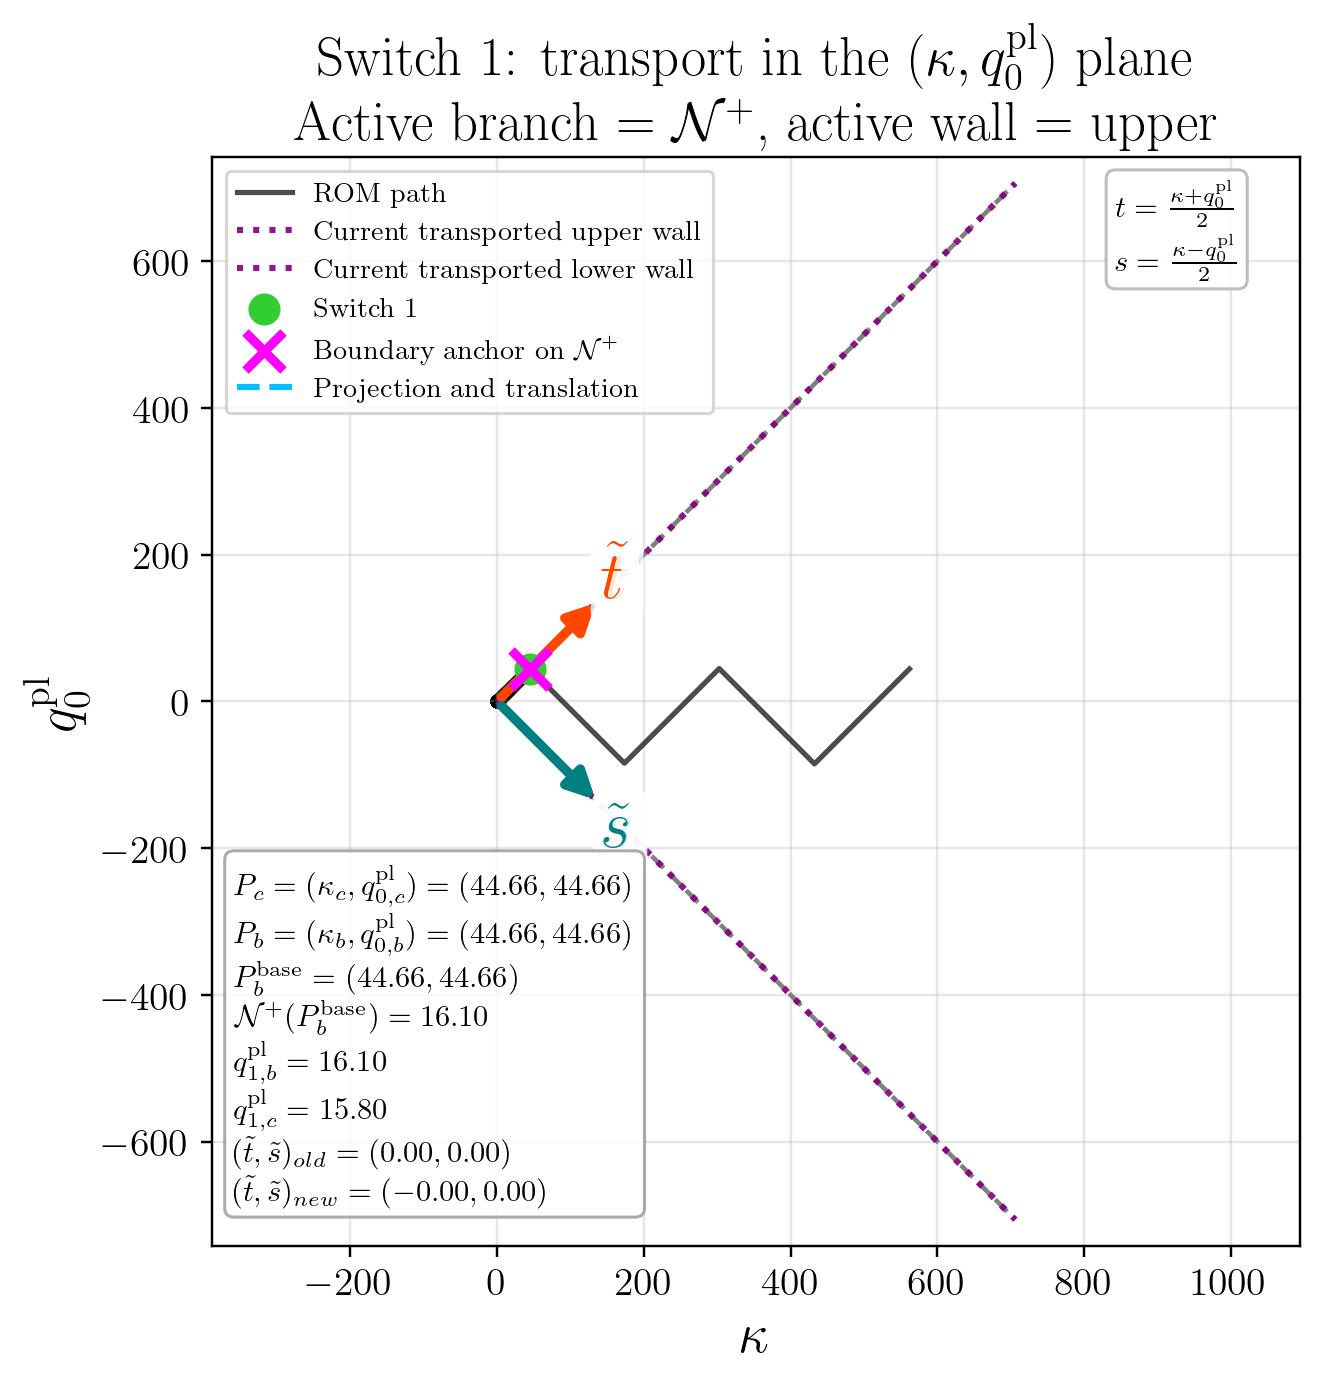
\includegraphics[width=\textwidth]{two_surface_switch_with_boundary_projection_transport/switch_001_xy_projection.png}
\caption{Projection in the \((\kappa,q^{\mathrm{pl}}_0)\) plane.}
\end{subfigure}
\hfill
\begin{subfigure}{0.47\textwidth}
\centering
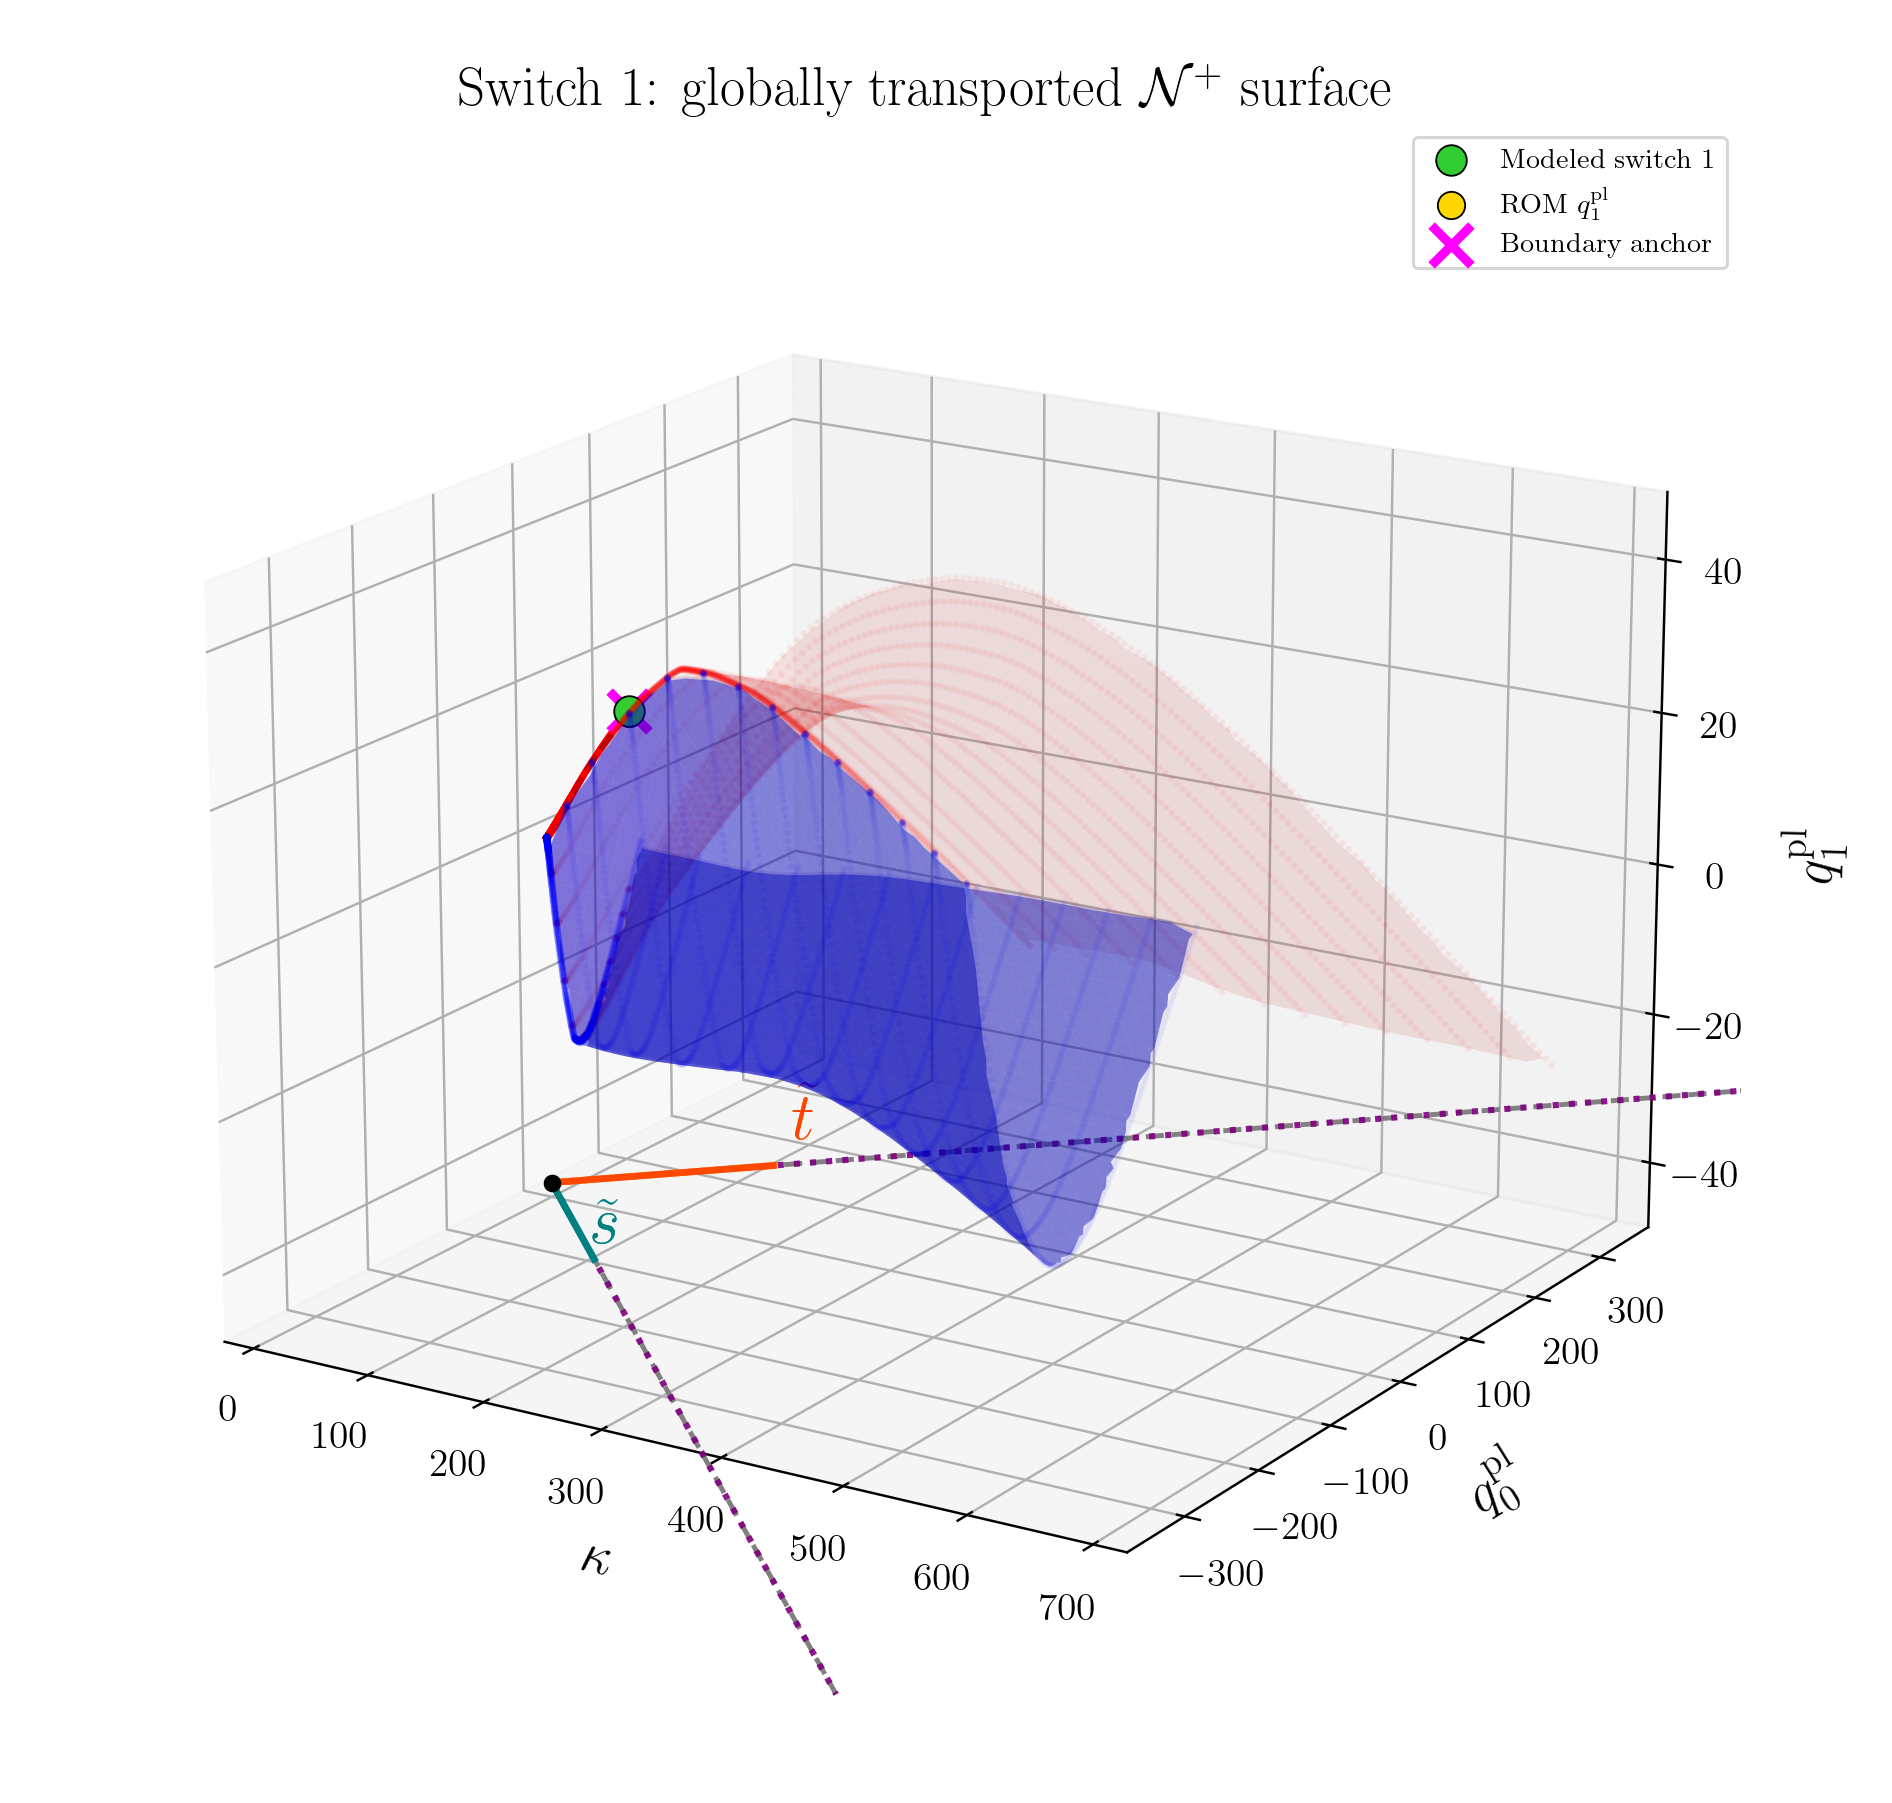
\includegraphics[width=\textwidth]{two_surface_switch_with_boundary_projection_transport/switch_001_transport_view1.png}
\caption{Transported \(\mathcal{N}^{+}\) surface in latent space.}
\end{subfigure}
\caption{Worked example for Switch 1. Since \(P_c\) already lies on the active upper wall, the projection is trivial and the update consists only of a vertical re-anchoring of the branch \(\mathcal{N}^{+}\).}
\label{fig:tutorial_switch1}
\end{figure}

\subsection{Switch 2: activation of \texorpdfstring{$\mathcal{N}^{-}$}{N-}}

At the second switching event, the newly active branch is \(\mathcal{N}^{-}\), and the active wall is the transported lower wall. The switching point is
\begin{equation}
P_c
=
(\kappa_c,q^{\mathrm{pl}}_{0,c})
=
(173.56,\;-84.25).
\end{equation}
The old transported frame is still essentially the reference one,
\begin{equation}
(\tilde t,\tilde s)_{\mathrm{old}}=(0.00,\;0.00),
\end{equation}
so projection onto the lower wall is equivalent to setting \(t=0\) while keeping \(s\) fixed. In the \((t,s)\) variables, the switching point is reported as
\begin{equation}
(t_c,s_c)=(44.66,\;128.91).
\end{equation}
Hence the boundary anchor is
\begin{equation}
(t_b,s_b)=(0.00,\;128.91),
\end{equation}
which in the \((\kappa,q^{\mathrm{pl}}_0)\) coordinates becomes
\begin{equation}
P_b=(128.91,\;-128.91).
\end{equation}
Since the old transport was zero, the base coordinates on the newly activated branch are again
\begin{equation}
P_b^{\mathrm{base}}=(128.91,\;-128.91).
\end{equation}
Evaluating the red branch there gives
\begin{equation}
\mathcal{N}^{-}(P_b^{\mathrm{base}})=-13.58,
\end{equation}
and the transported value at the boundary anchor is reported as
\begin{equation}
q^{\mathrm{pl}}_{1,b}=-13.41.
\end{equation}
The ROM value at the switching point is
\begin{equation}
q^{\mathrm{pl}}_{1,c}=-20.58.
\end{equation}
Thus the vertical correction of the newly activated branch is
\begin{equation}
\Delta q^{\mathrm{pl}}_{1,-}
=
q^{\mathrm{pl}}_{1,c}-q^{\mathrm{pl}}_{1,b}
=
-20.58-(-13.41)
=
-7.17.
\end{equation}
Now the in-plane update is nontrivial. The projection moved the point from \(P_c\) to \(P_b\), so the transported frame must be translated by
\begin{equation}
(\Delta \kappa,\Delta q^{\mathrm{pl}}_0)
=
(\kappa_c-\kappa_b,\;q^{\mathrm{pl}}_{0,c}-q^{\mathrm{pl}}_{0,b})
=
(44.66,\;44.66).
\end{equation}
Equivalently,
\begin{equation}
(\tilde t,\tilde s)_{\mathrm{new}}=(44.66,\;0.00).
\end{equation}

So Switch 2 is the first genuinely nontrivial example: one first projects onto the lower wall, then translates the whole wedge in-plane, and finally lowers the branch \(\mathcal{N}^{-}\) so that it matches the ROM value at the switch.

\begin{figure}[H]
\centering
\begin{subfigure}{0.47\textwidth}
\centering
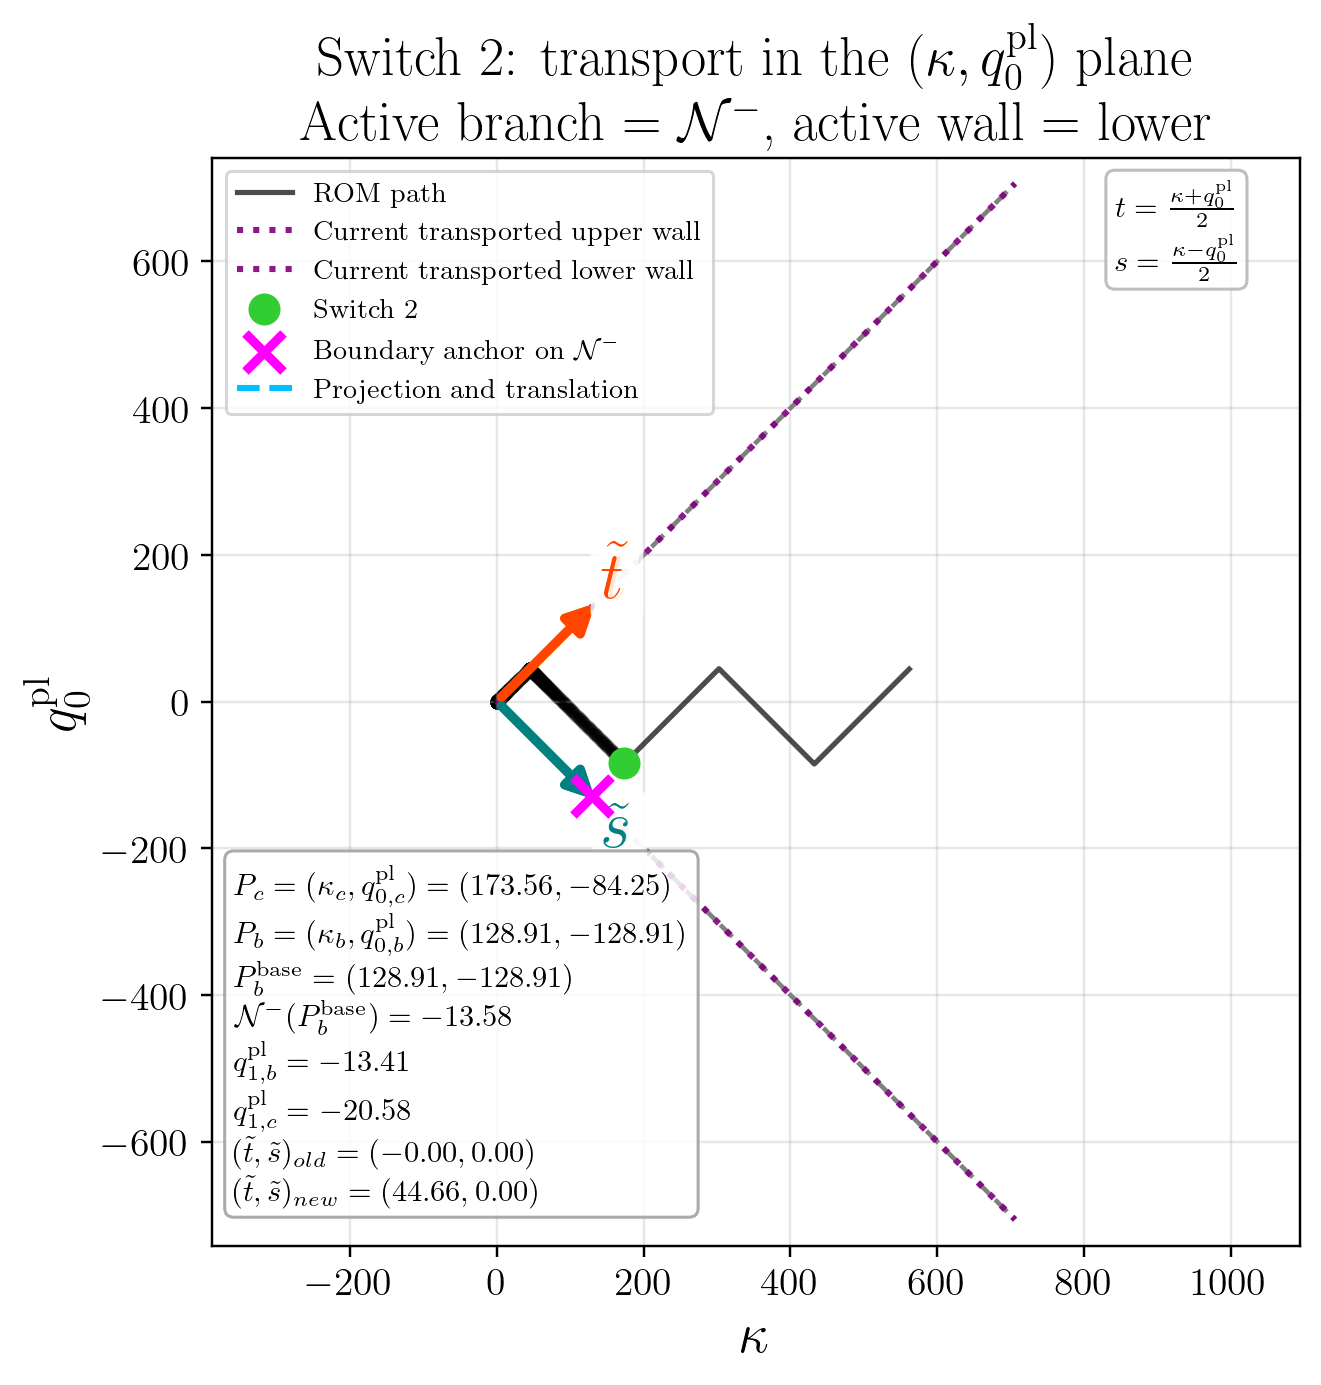
\includegraphics[width=\textwidth]{two_surface_switch_with_boundary_projection_transport/switch_002_xy_projection.png}
\caption{Projection in the \((\kappa,q^{\mathrm{pl}}_0)\) plane.}
\end{subfigure}
\hfill
\begin{subfigure}{0.47\textwidth}
\centering
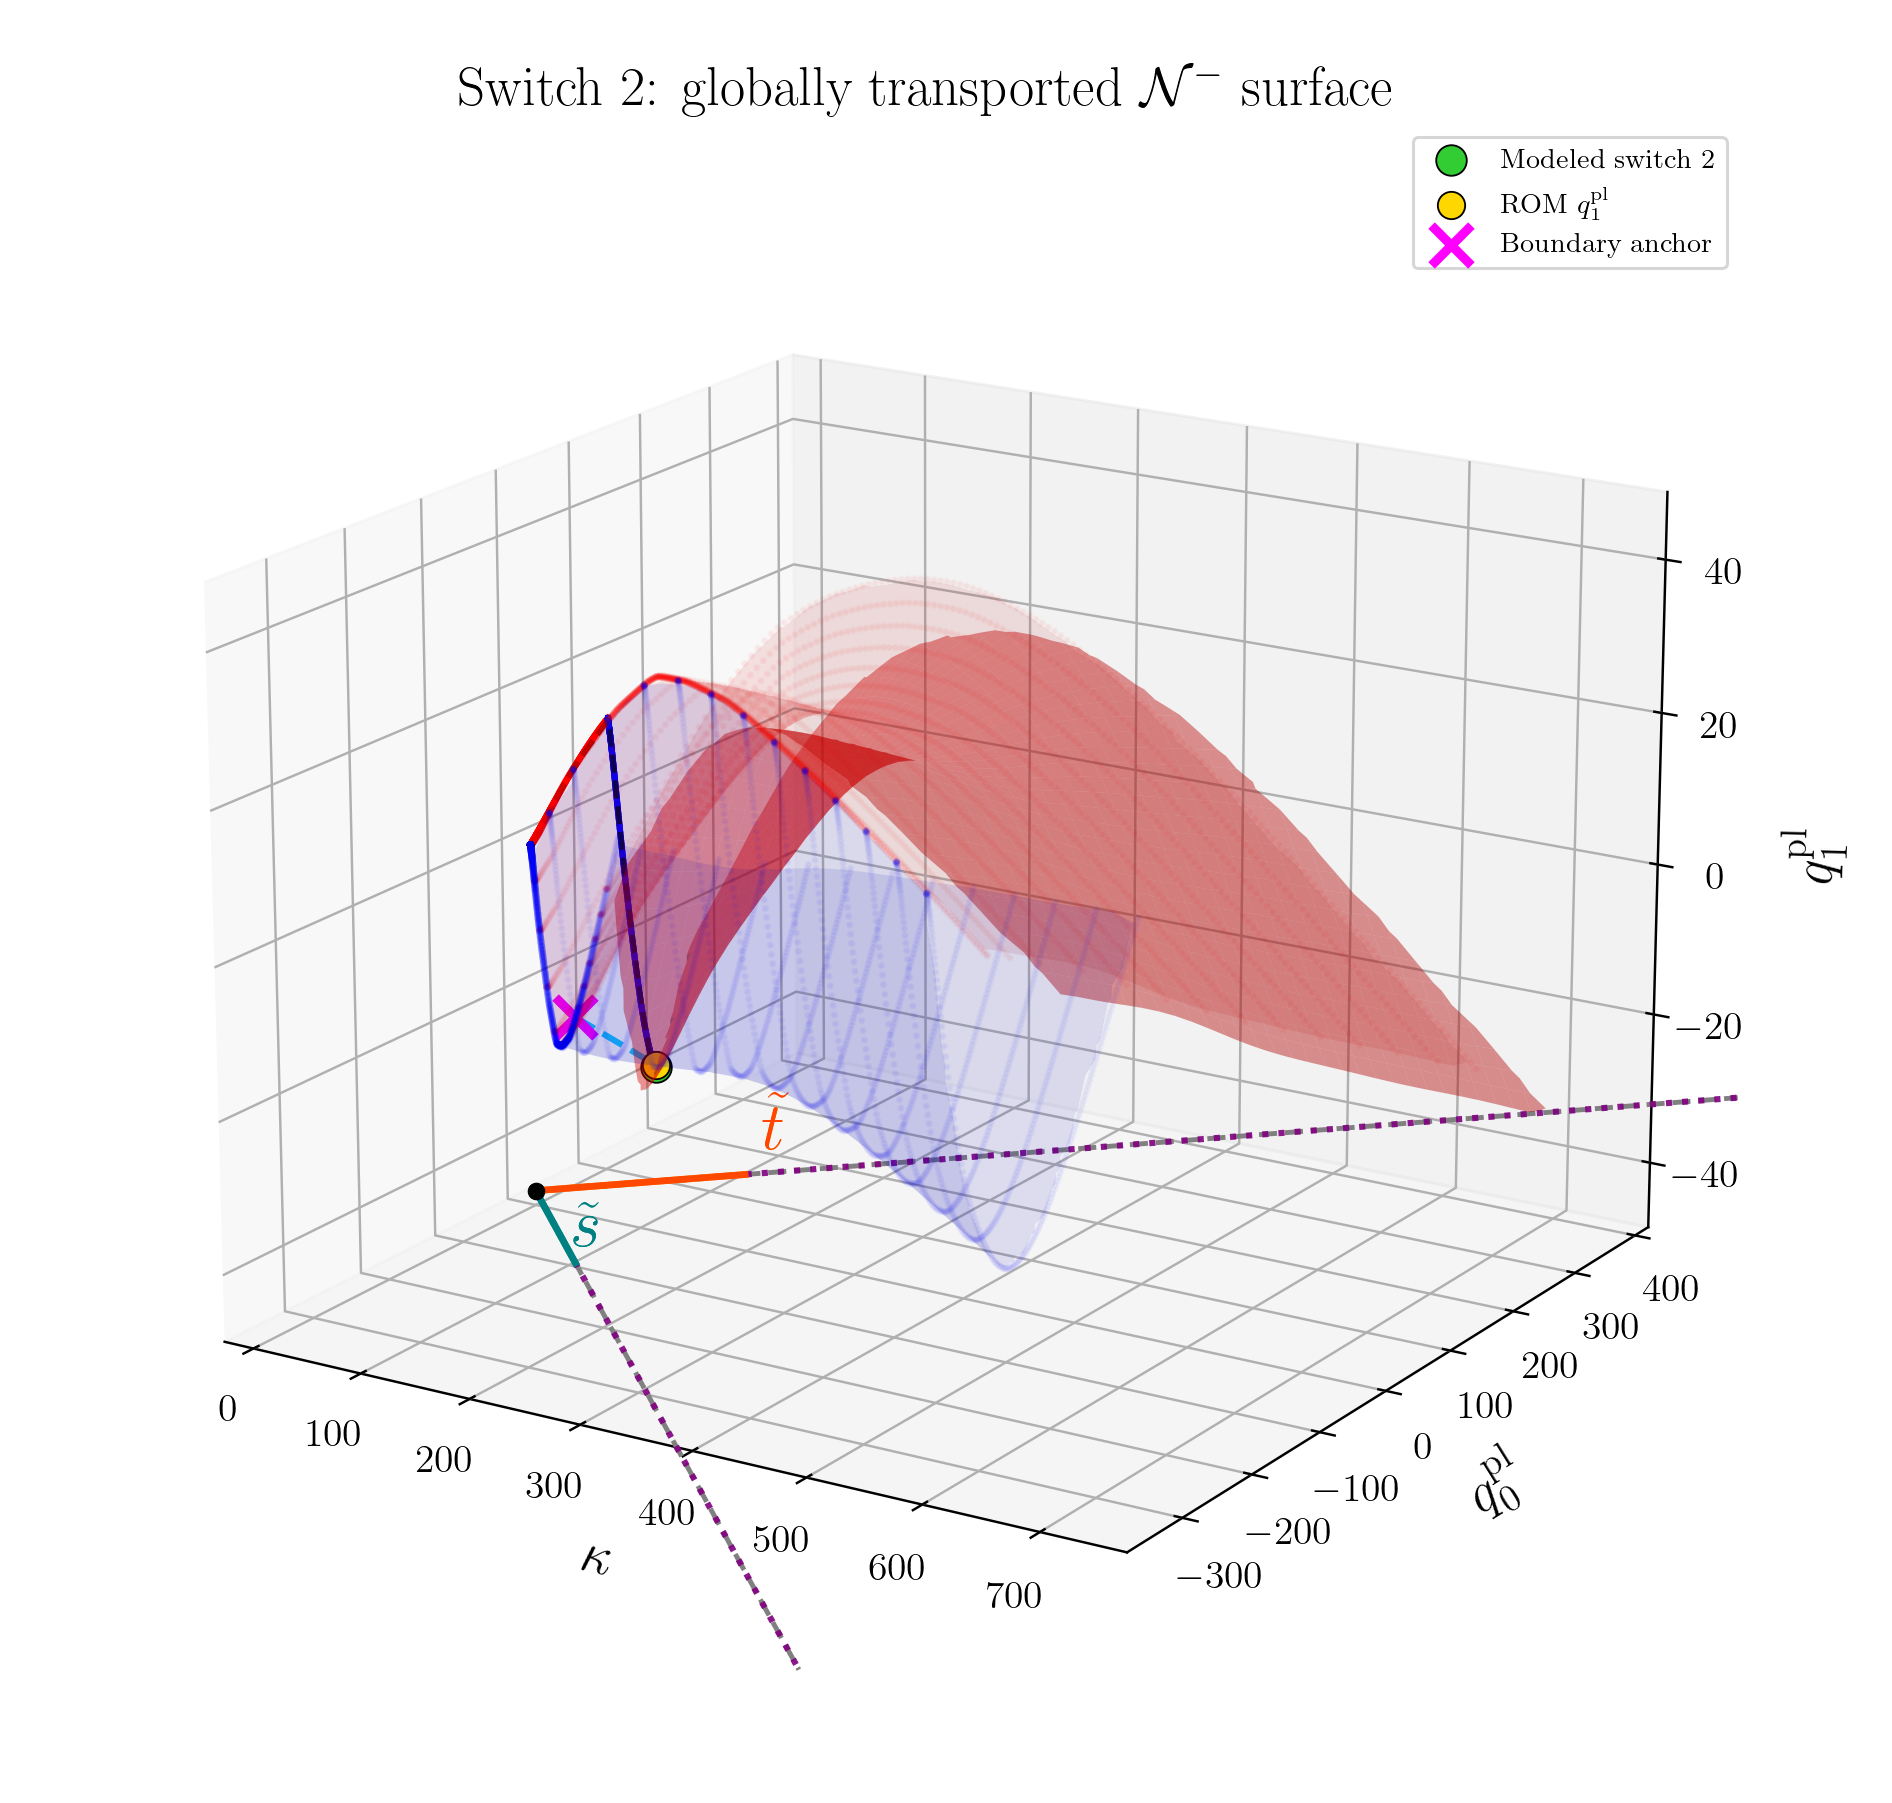
\includegraphics[width=\textwidth]{two_surface_switch_with_boundary_projection_transport/switch_002_transport_view1.png}
\caption{Transported \(\mathcal{N}^{-}\) surface in latent space.}
\end{subfigure}
\caption{Worked example for Switch 2. The point is projected onto the lower wall, the latent frame is translated by \((44.66,44.66)\), and the red branch is vertically corrected to pass through the ROM switch value.}
\label{fig:tutorial_switch2}
\end{figure}

\subsection{Switch 3: re-activation of \texorpdfstring{$\mathcal{N}^{+}$}{N+}}

At Switch 3, the active branch changes back to \(\mathcal{N}^{+}\), now with a nonzero transported frame already in place. The switching point is
\begin{equation}
P_c=(302.64,\;44.82),
\end{equation}
and in the \((t,s)\) variables it is reported as
\begin{equation}
(t_c,s_c)=(173.73,\;128.91).
\end{equation}
The old transported frame is
\begin{equation}
(\tilde t,\tilde s)_{\mathrm{old}}=(44.66,\;0.00).
\end{equation}
Since the new active wall is the upper wall, projection keeps \(t\) fixed and sets \(s=\tilde s_{\mathrm{old}}=0\). Hence
\begin{equation}
(t_b,s_b)=(173.73,\;0.00),
\end{equation}
which corresponds to
\begin{equation}
P_b=(173.73,\;173.73).
\end{equation}
In the fixed coordinates of the newly activated blue branch, the base anchor is
\begin{equation}
P_b^{\mathrm{base}}=(129.08,\;129.08).
\end{equation}
Evaluation of the blue surface there gives
\begin{equation}
\mathcal{N}^{+}(P_b^{\mathrm{base}})=13.54.
\end{equation}
The transported branch value at the anchor is
\begin{equation}
q^{\mathrm{pl}}_{1,b}=13.24,
\end{equation}
whereas the ROM value at the switching point is
\begin{equation}
q^{\mathrm{pl}}_{1,c}=19.74.
\end{equation}
Therefore the vertical increment on the blue branch is
\begin{equation}
\Delta q^{\mathrm{pl}}_{1,+}
=
19.74-13.24
=
6.50.
\end{equation}
The in-plane translation is now
\begin{equation}
(\Delta \kappa,\Delta q^{\mathrm{pl}}_0)
=
(302.64-173.73,\;44.82-173.73)
=
(128.91,\;-128.91),
\end{equation}
which is equivalent to
\begin{equation}
(\tilde t,\tilde s)_{\mathrm{new}}=(44.66,\;128.91).
\end{equation}

This switch is useful because it shows clearly that the transported quadrant no longer coincides with the reference wedge. One projects onto the wall of the already transported frame, not onto the original wall.

\begin{figure}[H]
\centering
\begin{subfigure}{0.47\textwidth}
\centering
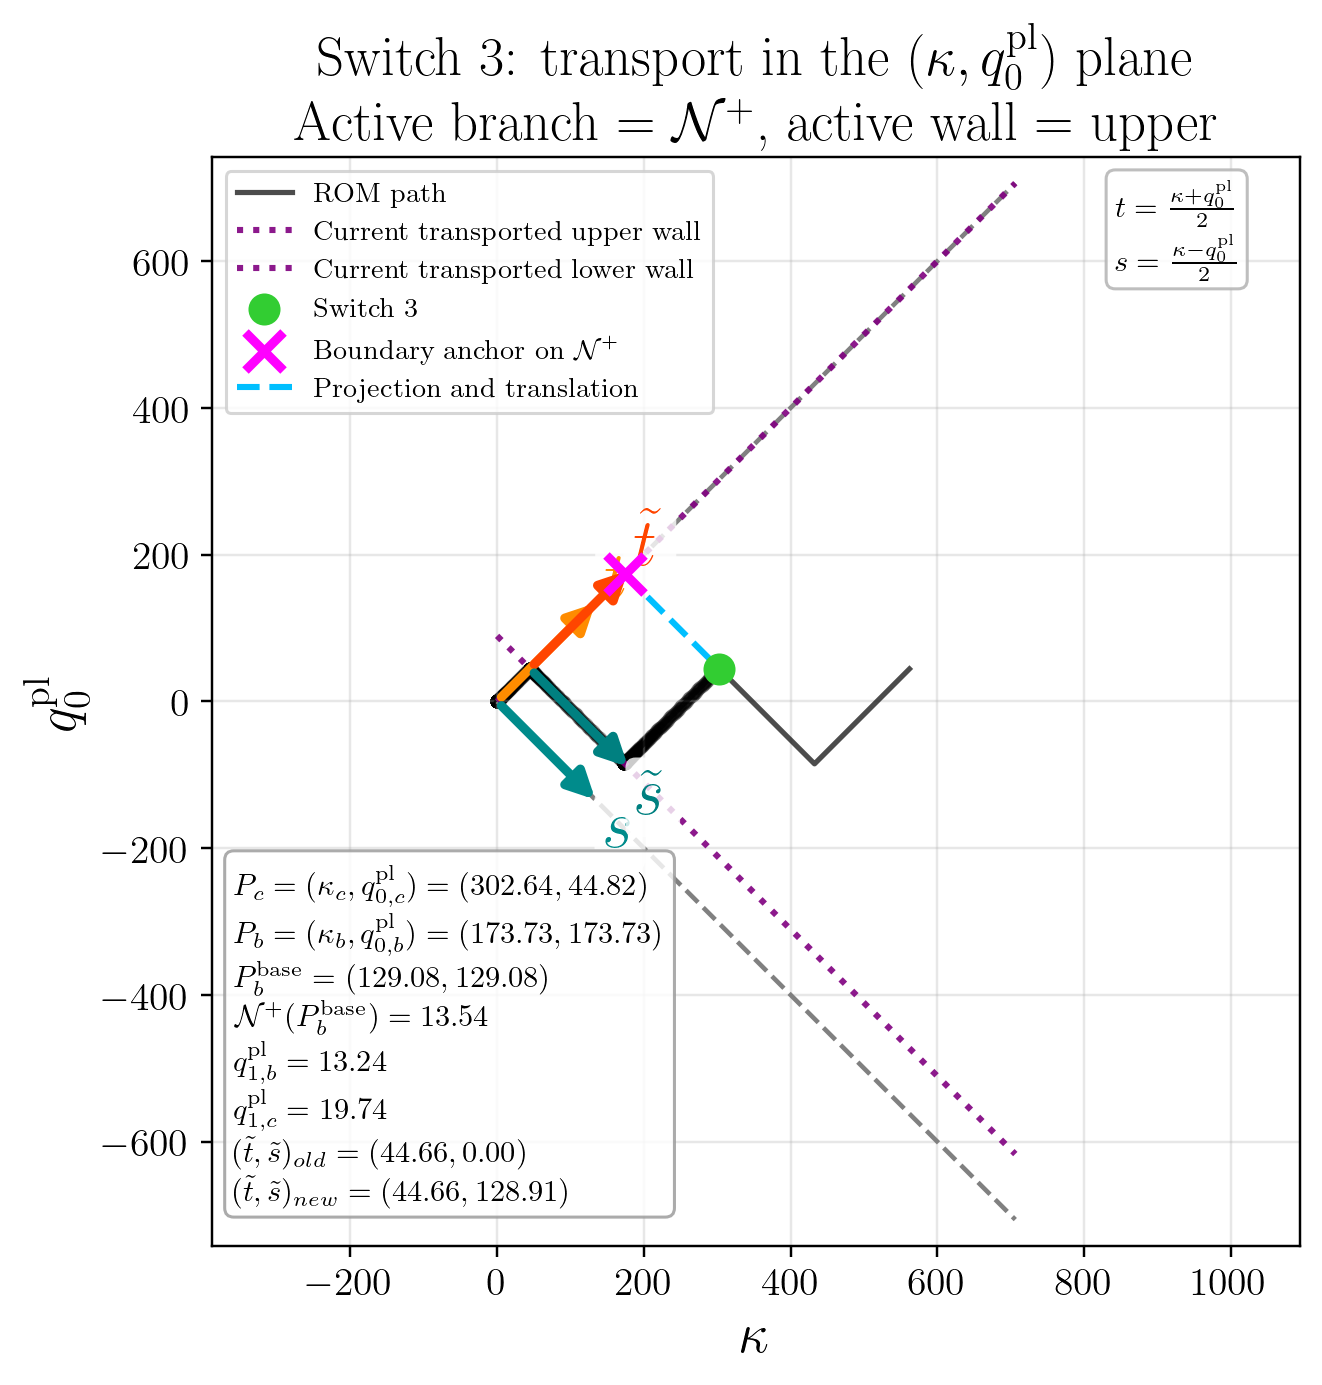
\includegraphics[width=\textwidth]{two_surface_switch_with_boundary_projection_transport/switch_003_xy_projection.png}
\caption{Projection in the \((\kappa,q^{\mathrm{pl}}_0)\) plane.}
\end{subfigure}
\hfill
\begin{subfigure}{0.47\textwidth}
\centering
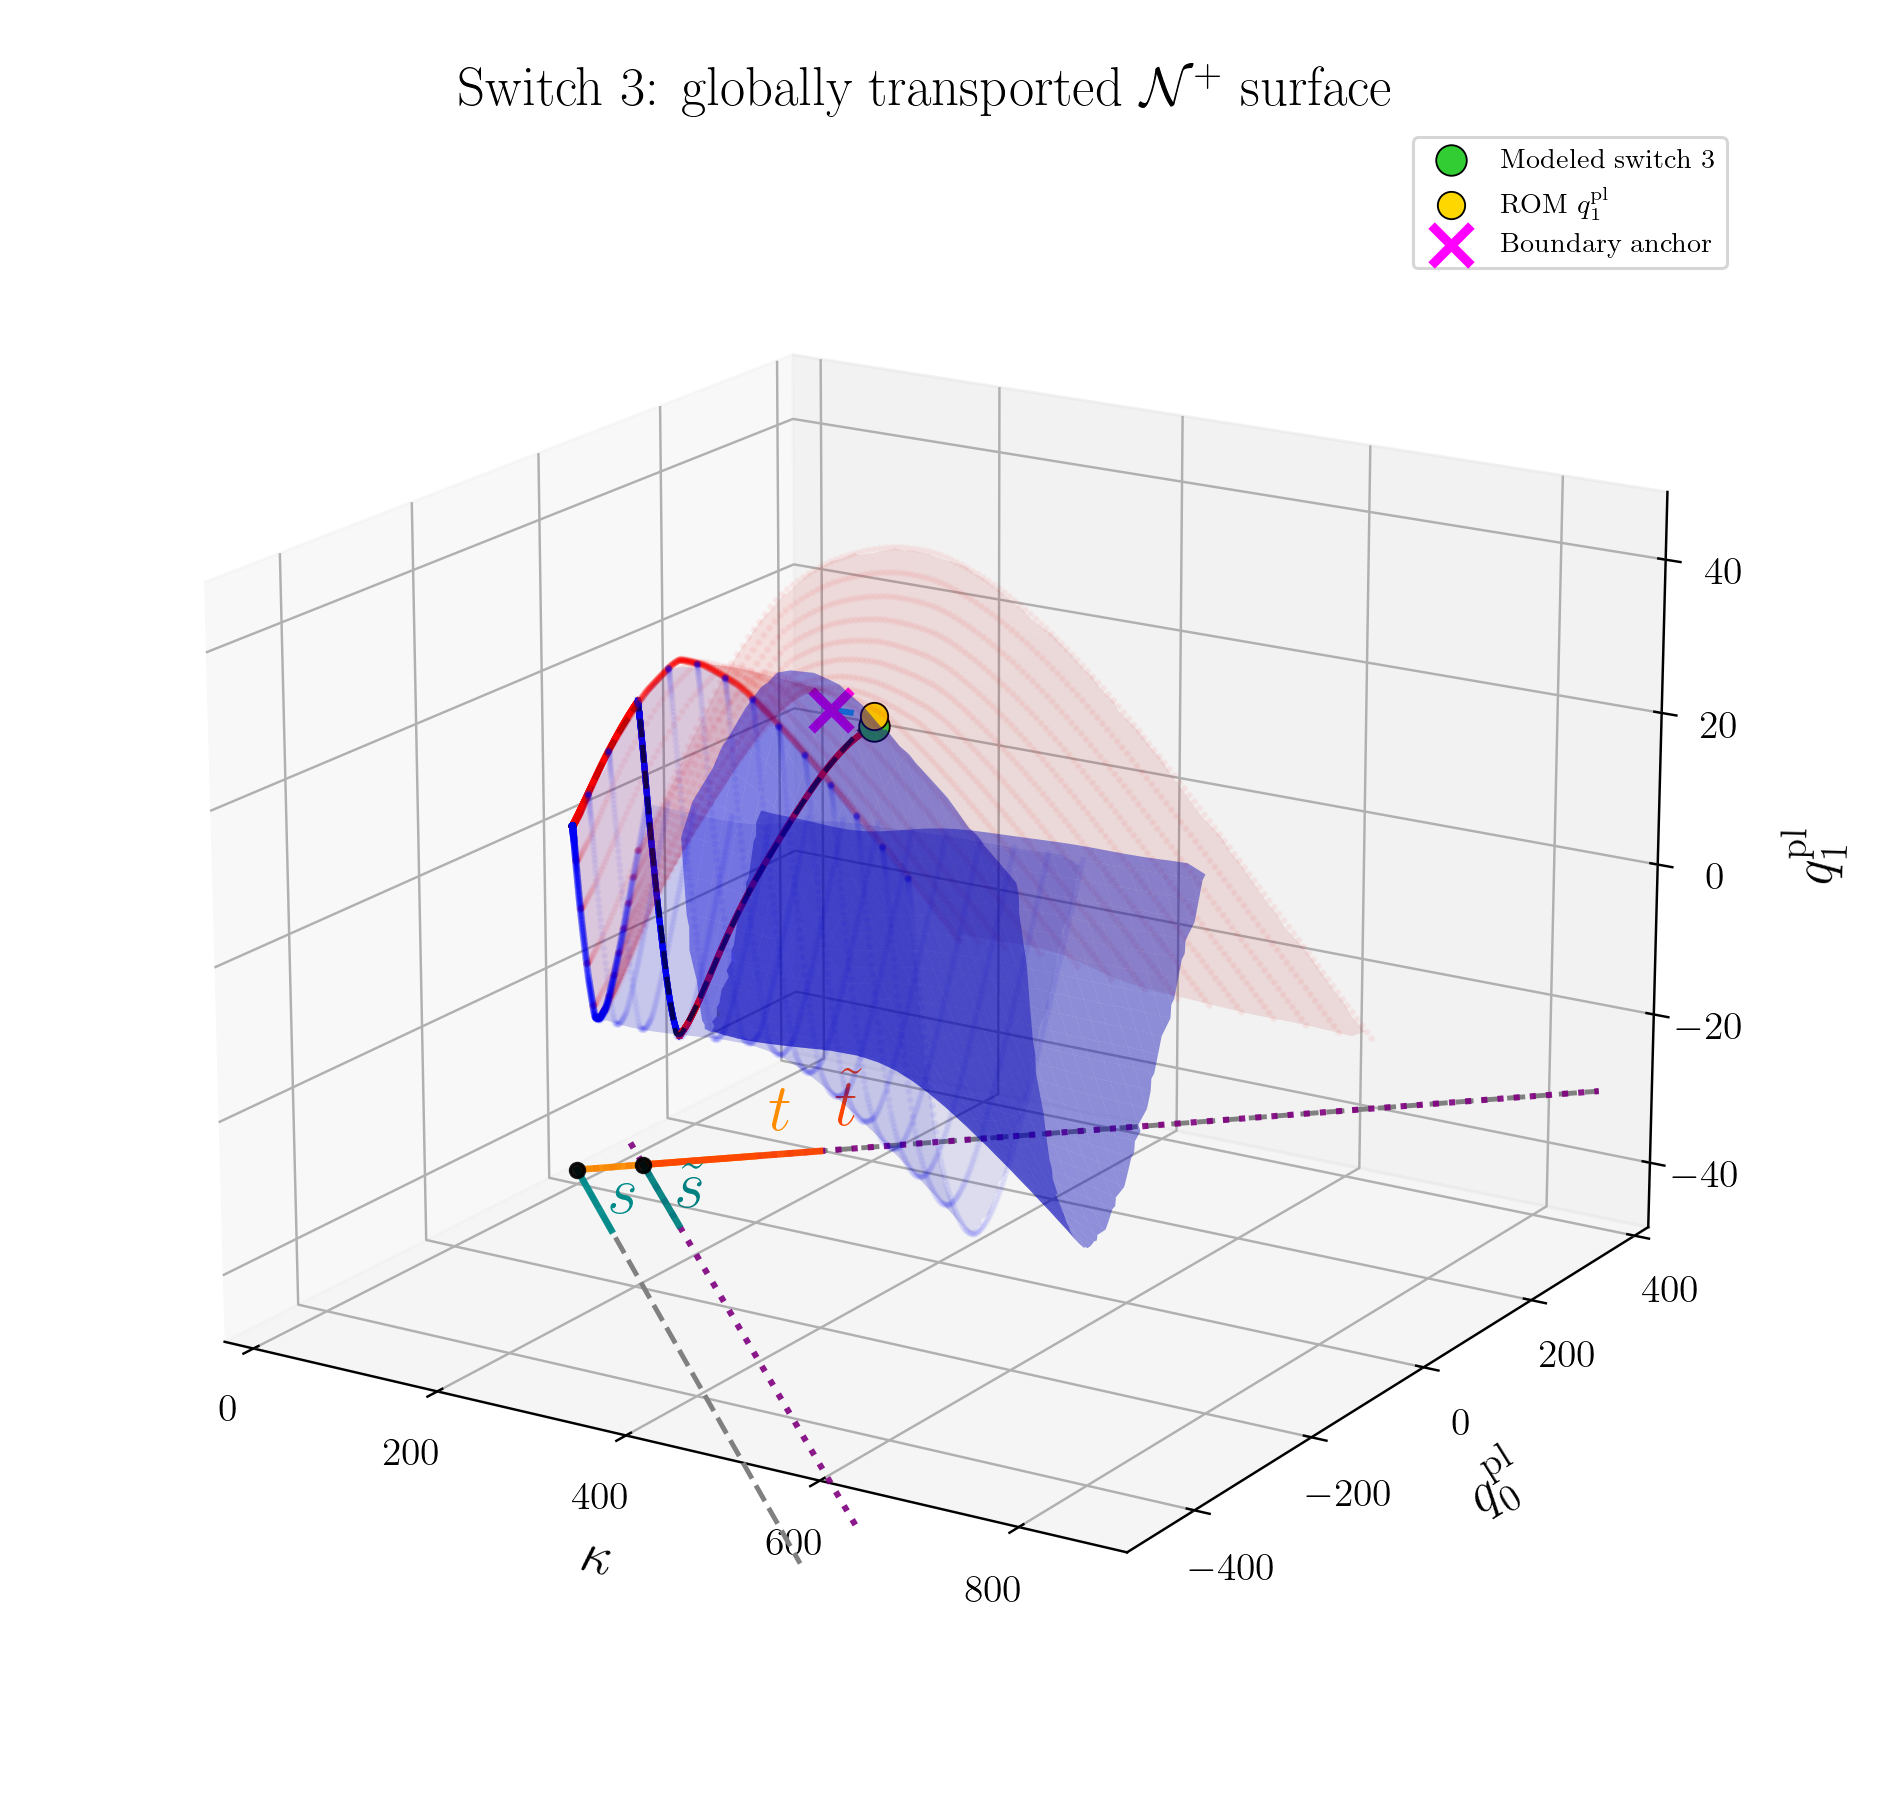
\includegraphics[width=\textwidth]{two_surface_switch_with_boundary_projection_transport/switch_003_transport_view1.png}
\caption{Transported \(\mathcal{N}^{+}\) surface in latent space.}
\end{subfigure}
\caption{Worked example for Switch 3. The projection is performed onto the upper wall of the already transported frame, after which the blue branch is translated and vertically re-anchored.}
\label{fig:tutorial_switch3}
\end{figure}

\subsection{Switch 4: re-activation of \texorpdfstring{$\mathcal{N}^{-}$}{N-}}

At the fourth switch, the active branch returns to \(\mathcal{N}^{-}\). The switching point is
\begin{equation}
P_c=(432.59,\;-85.13),
\end{equation}
with transformed coordinates
\begin{equation}
(t_c,s_c)=(173.73,\;258.86).
\end{equation}
The old transported frame before this switch is
\begin{equation}
(\tilde t,\tilde s)_{\mathrm{old}}=(44.66,\;128.91).
\end{equation}
Since the new active wall is the lower wall, projection sets \(t=\tilde t_{\mathrm{old}}=44.66\) and keeps \(s\) fixed:
\begin{equation}
(t_b,s_b)=(44.66,\;258.86).
\end{equation}
In the original variables this gives
\begin{equation}
P_b=(303.51,\;-214.20).
\end{equation}
After mapping back to the fixed coordinates of the red surface, the base point is
\begin{equation}
P_b^{\mathrm{base}}=(129.95,\;-129.95).
\end{equation}
Evaluating the red branch there gives
\begin{equation}
\mathcal{N}^{-}(P_b^{\mathrm{base}})=-13.35.
\end{equation}
The transported value at the anchor is
\begin{equation}
q^{\mathrm{pl}}_{1,b}=-20.35,
\end{equation}
while the ROM value at the switching point is
\begin{equation}
q^{\mathrm{pl}}_{1,c}=-20.36.
\end{equation}
Hence the vertical correction is almost zero:
\begin{equation}
\Delta q^{\mathrm{pl}}_{1,-}
=
-20.36-(-20.35)
\approx
0.00.
\end{equation}
The in-plane update is
\begin{equation}
(\Delta \kappa,\Delta q^{\mathrm{pl}}_0)
=
(432.59-303.51,\;-85.13-(-214.20))
=
(129.08,\;129.08),
\end{equation}
which yields the new transported frame
\begin{equation}
(\tilde t,\tilde s)_{\mathrm{new}}=(173.73,\;128.91).
\end{equation}

This last switch is informative because it shows a case in which the new branch is already almost vertically aligned with the ROM value. The essential update is therefore in-plane rather than vertical.

\begin{figure}[H]
\centering
\begin{subfigure}{0.47\textwidth}
\centering
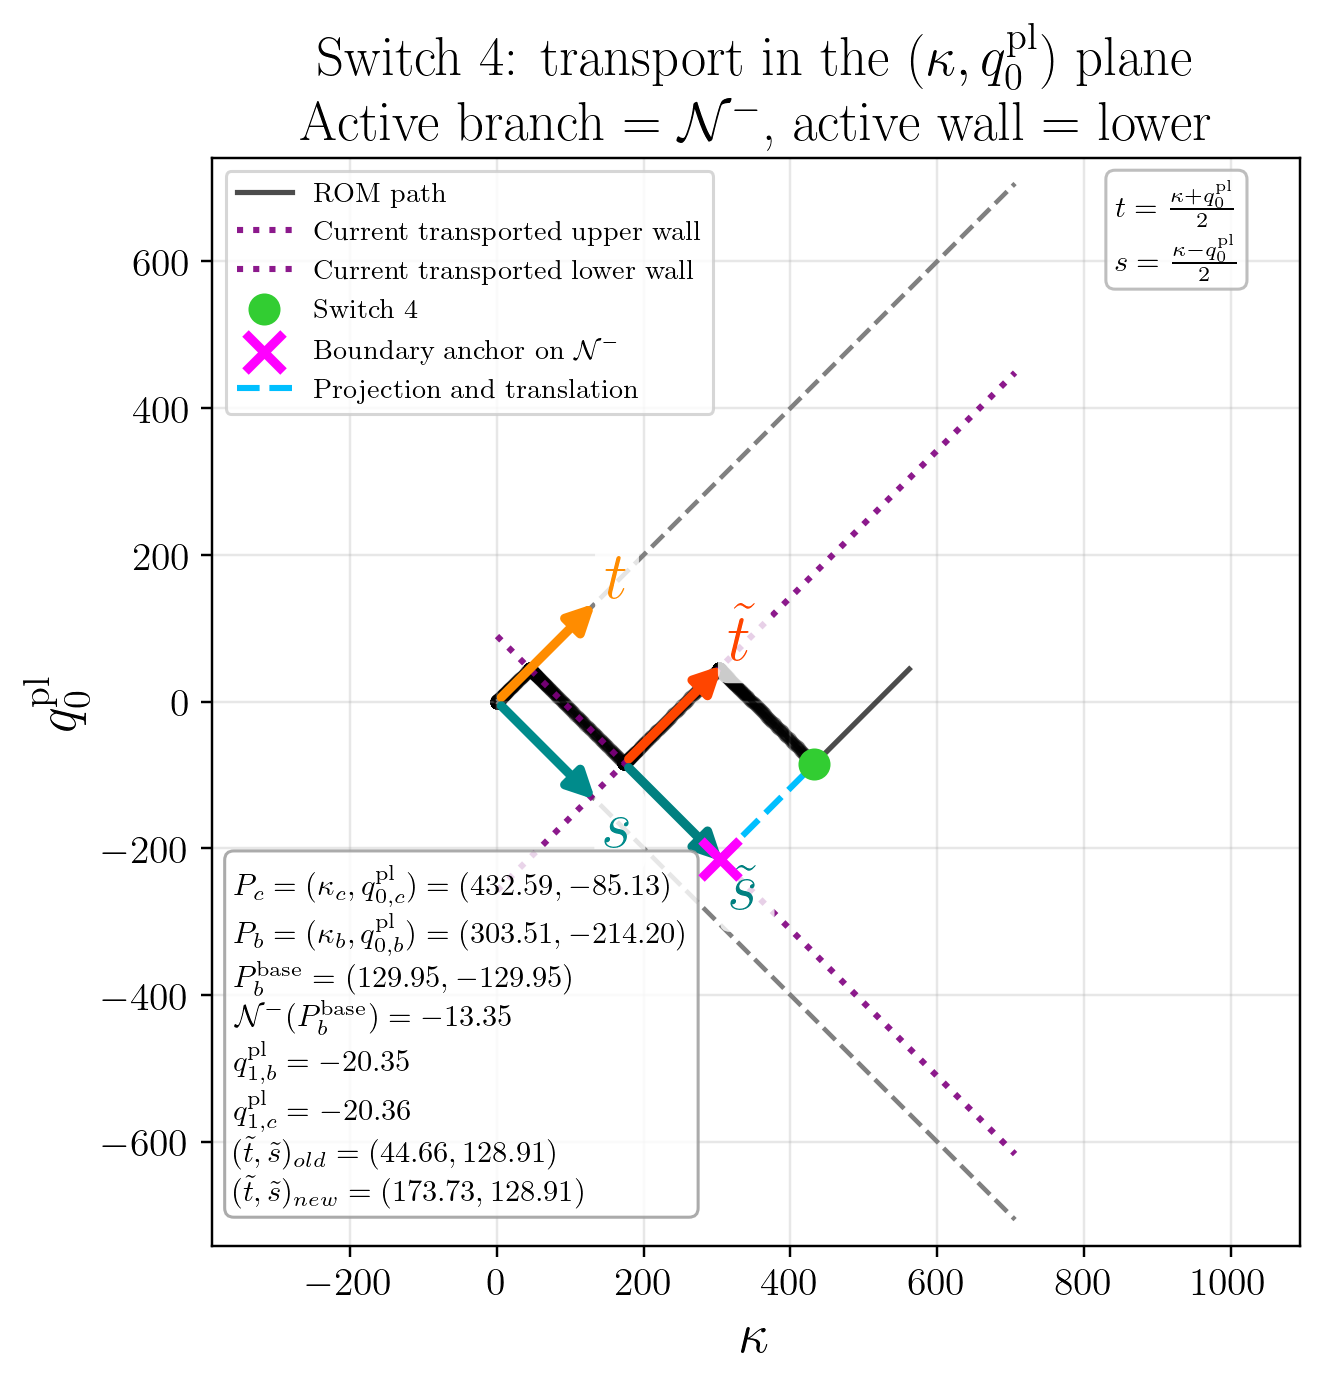
\includegraphics[width=\textwidth]{two_surface_switch_with_boundary_projection_transport/switch_004_xy_projection.png}
\caption{Projection in the \((\kappa,q^{\mathrm{pl}}_0)\) plane.}
\end{subfigure}
\hfill
\begin{subfigure}{0.47\textwidth}
\centering
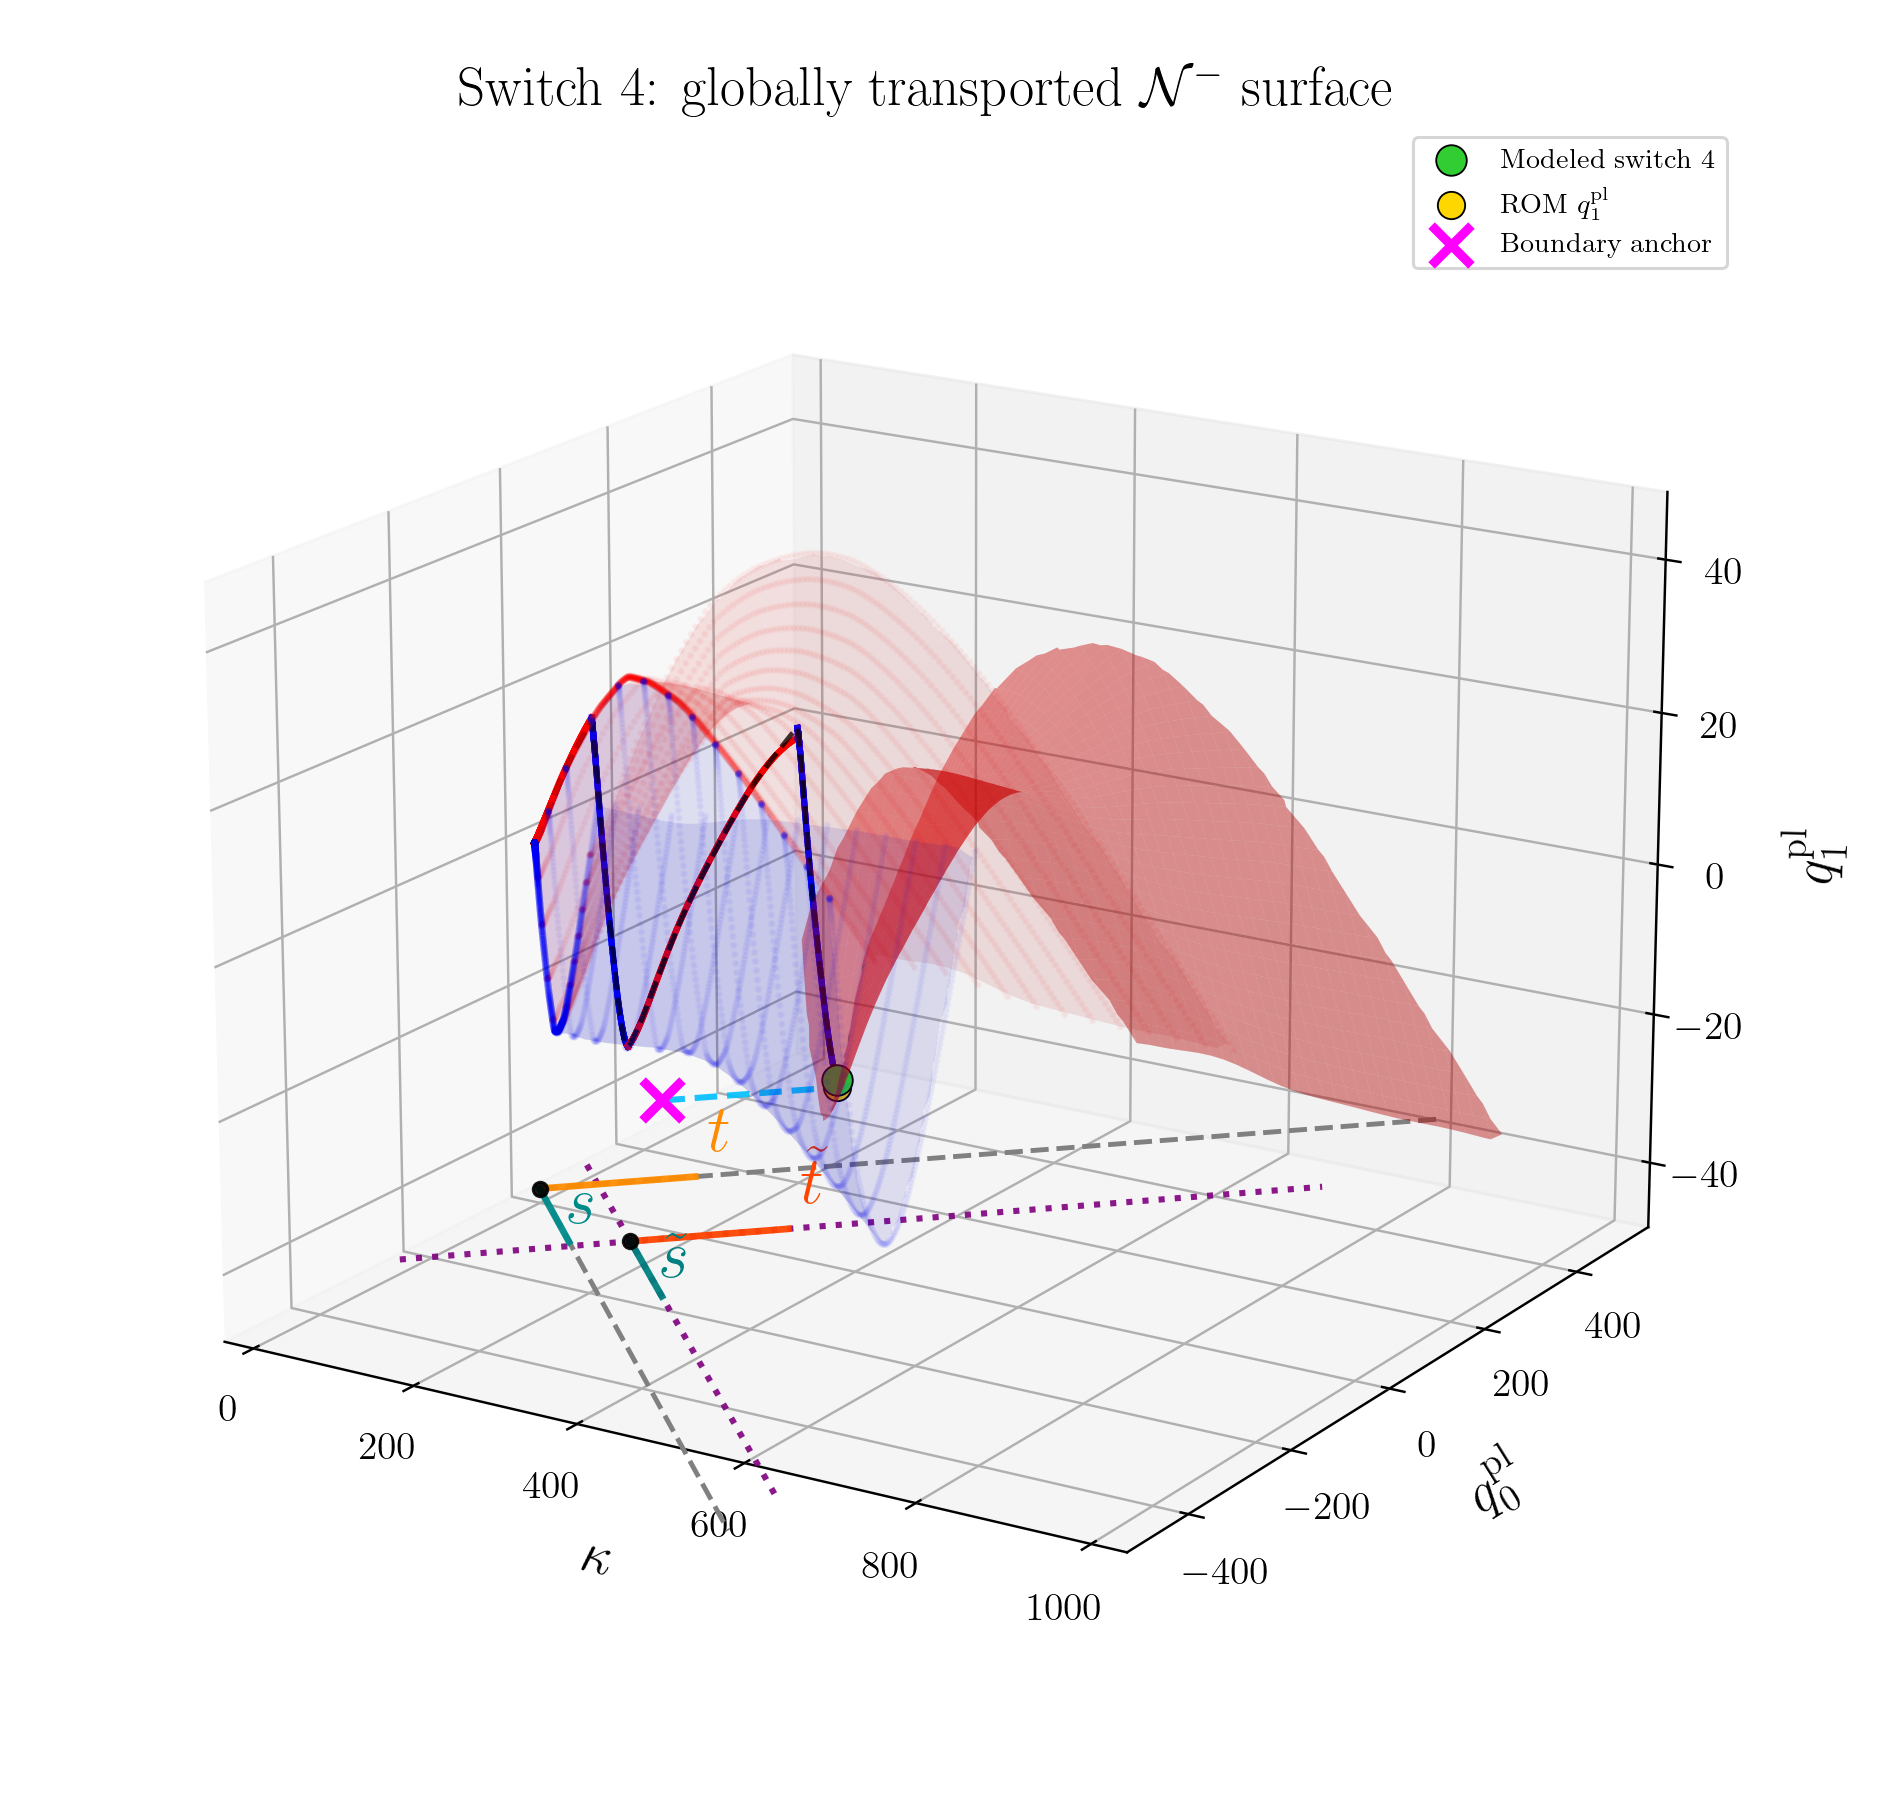
\includegraphics[width=\textwidth]{two_surface_switch_with_boundary_projection_transport/switch_004_transport_view1.png}
\caption{Transported \(\mathcal{N}^{-}\) surface in latent space.}
\end{subfigure}
\caption{Worked example for Switch 4. The red branch is activated again. The vertical correction is negligible, while the in-plane frame translation remains essential.}
\label{fig:tutorial_switch4}
\end{figure}

\subsection{Final segment evaluation after the last switch}

Once the last switch has been processed, the transport state is frozen again and the remaining path is evaluated on the transported active branch, exactly as in \eqref{eq:prediction_segment_explicit_transport_ref} or \eqref{eq:prediction_segment_explicit_ts_transport_ref}. The final active branch is \(\mathcal{N}^{-}\), and the final transport state is
\begin{equation}
(\Delta K,\Delta Q_0)_{\mathrm{final}}=(302.64,\;44.82),
\end{equation}
or equivalently
\begin{equation}
(\tilde t,\tilde s)_{\mathrm{final}}=(173.73,\;128.91).
\end{equation}

Consider the last evaluation point of the trajectory,
\begin{equation}
P_f=(\kappa_f,q^{\mathrm{pl}}_{0,f})=(561.98,\;44.27).
\end{equation}
Its transformed coordinates are reported as
\begin{equation}
(t_f,s_f)=(303.13,\;258.86).
\end{equation}
To evaluate the transported red branch, one first maps this point back to the fixed coordinates of the offline surface:
\begin{equation}
P_f^{\mathrm{base}}
=
(\kappa_f-\Delta K,\;q^{\mathrm{pl}}_{0,f}-\Delta Q_0)
=
(259.35,\;-0.56).
\end{equation}
Evaluating the red surface in those base coordinates gives
\begin{equation}
\mathcal{N}^{-}(P_f^{\mathrm{base}})=25.67.
\end{equation}
After applying the branch-specific vertical offset accumulated during the switches, the transported prediction becomes
\begin{equation}
q^{\mathrm{pl}}_{1,f,\mathrm{model}}=18.66.
\end{equation}
The corresponding ROM value is
\begin{equation}
q^{\mathrm{pl}}_{1,f,\mathrm{ROM}}=19.99.
\end{equation}

So the logic of the final evaluation is exactly the same as inside any branch segment:
\begin{enumerate}
\item take the current point in world coordinates,
\item map it back to the base coordinates of the active offline surface,
\item evaluate that surface,
\item add the branch-specific accumulated vertical offset.
\end{enumerate}

Nothing new happens after the last switch. The only difference is that the active frame is now the final transported frame resulting from all previous updates.

\begin{figure}[H]
\centering
\begin{subfigure}{0.47\textwidth}
\centering
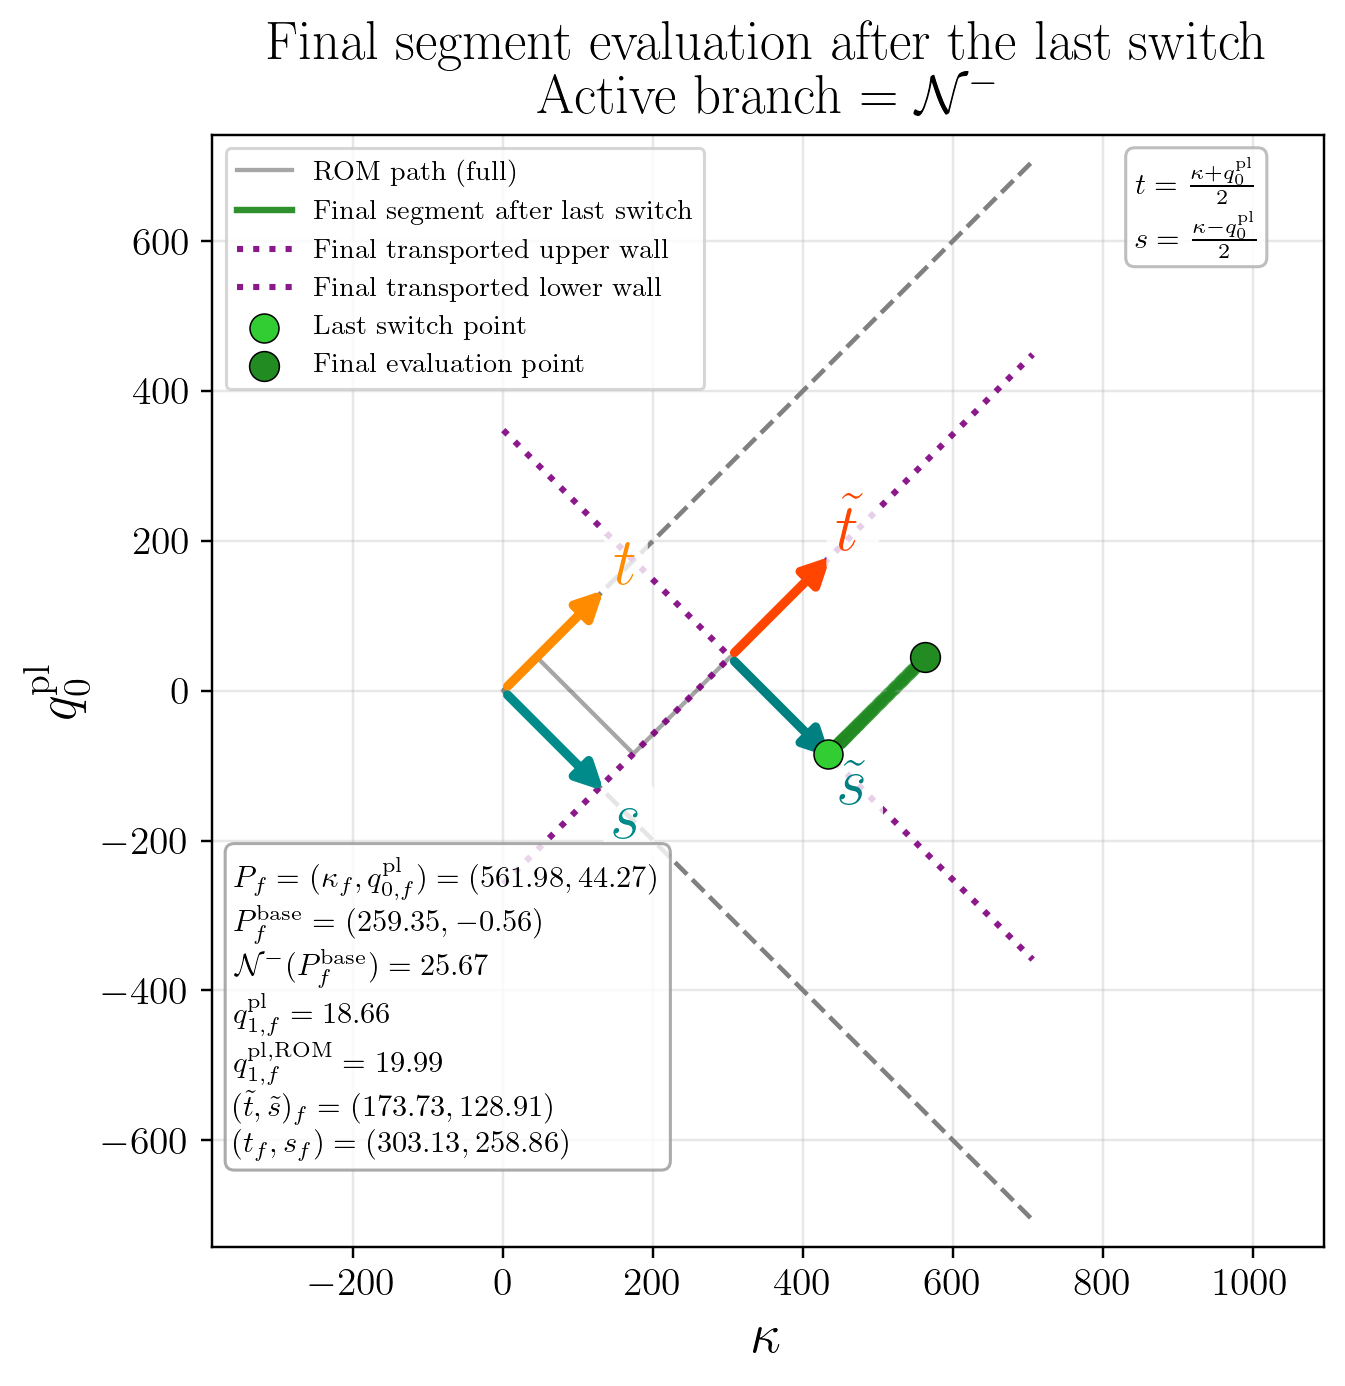
\includegraphics[width=\textwidth]{two_surface_switch_with_boundary_projection_transport/final_segment_xy_evaluation.png}
\caption{Final evaluation in the \((\kappa,q^{\mathrm{pl}}_0)\) plane.}
\end{subfigure}
\hfill
\begin{subfigure}{0.47\textwidth}
\centering
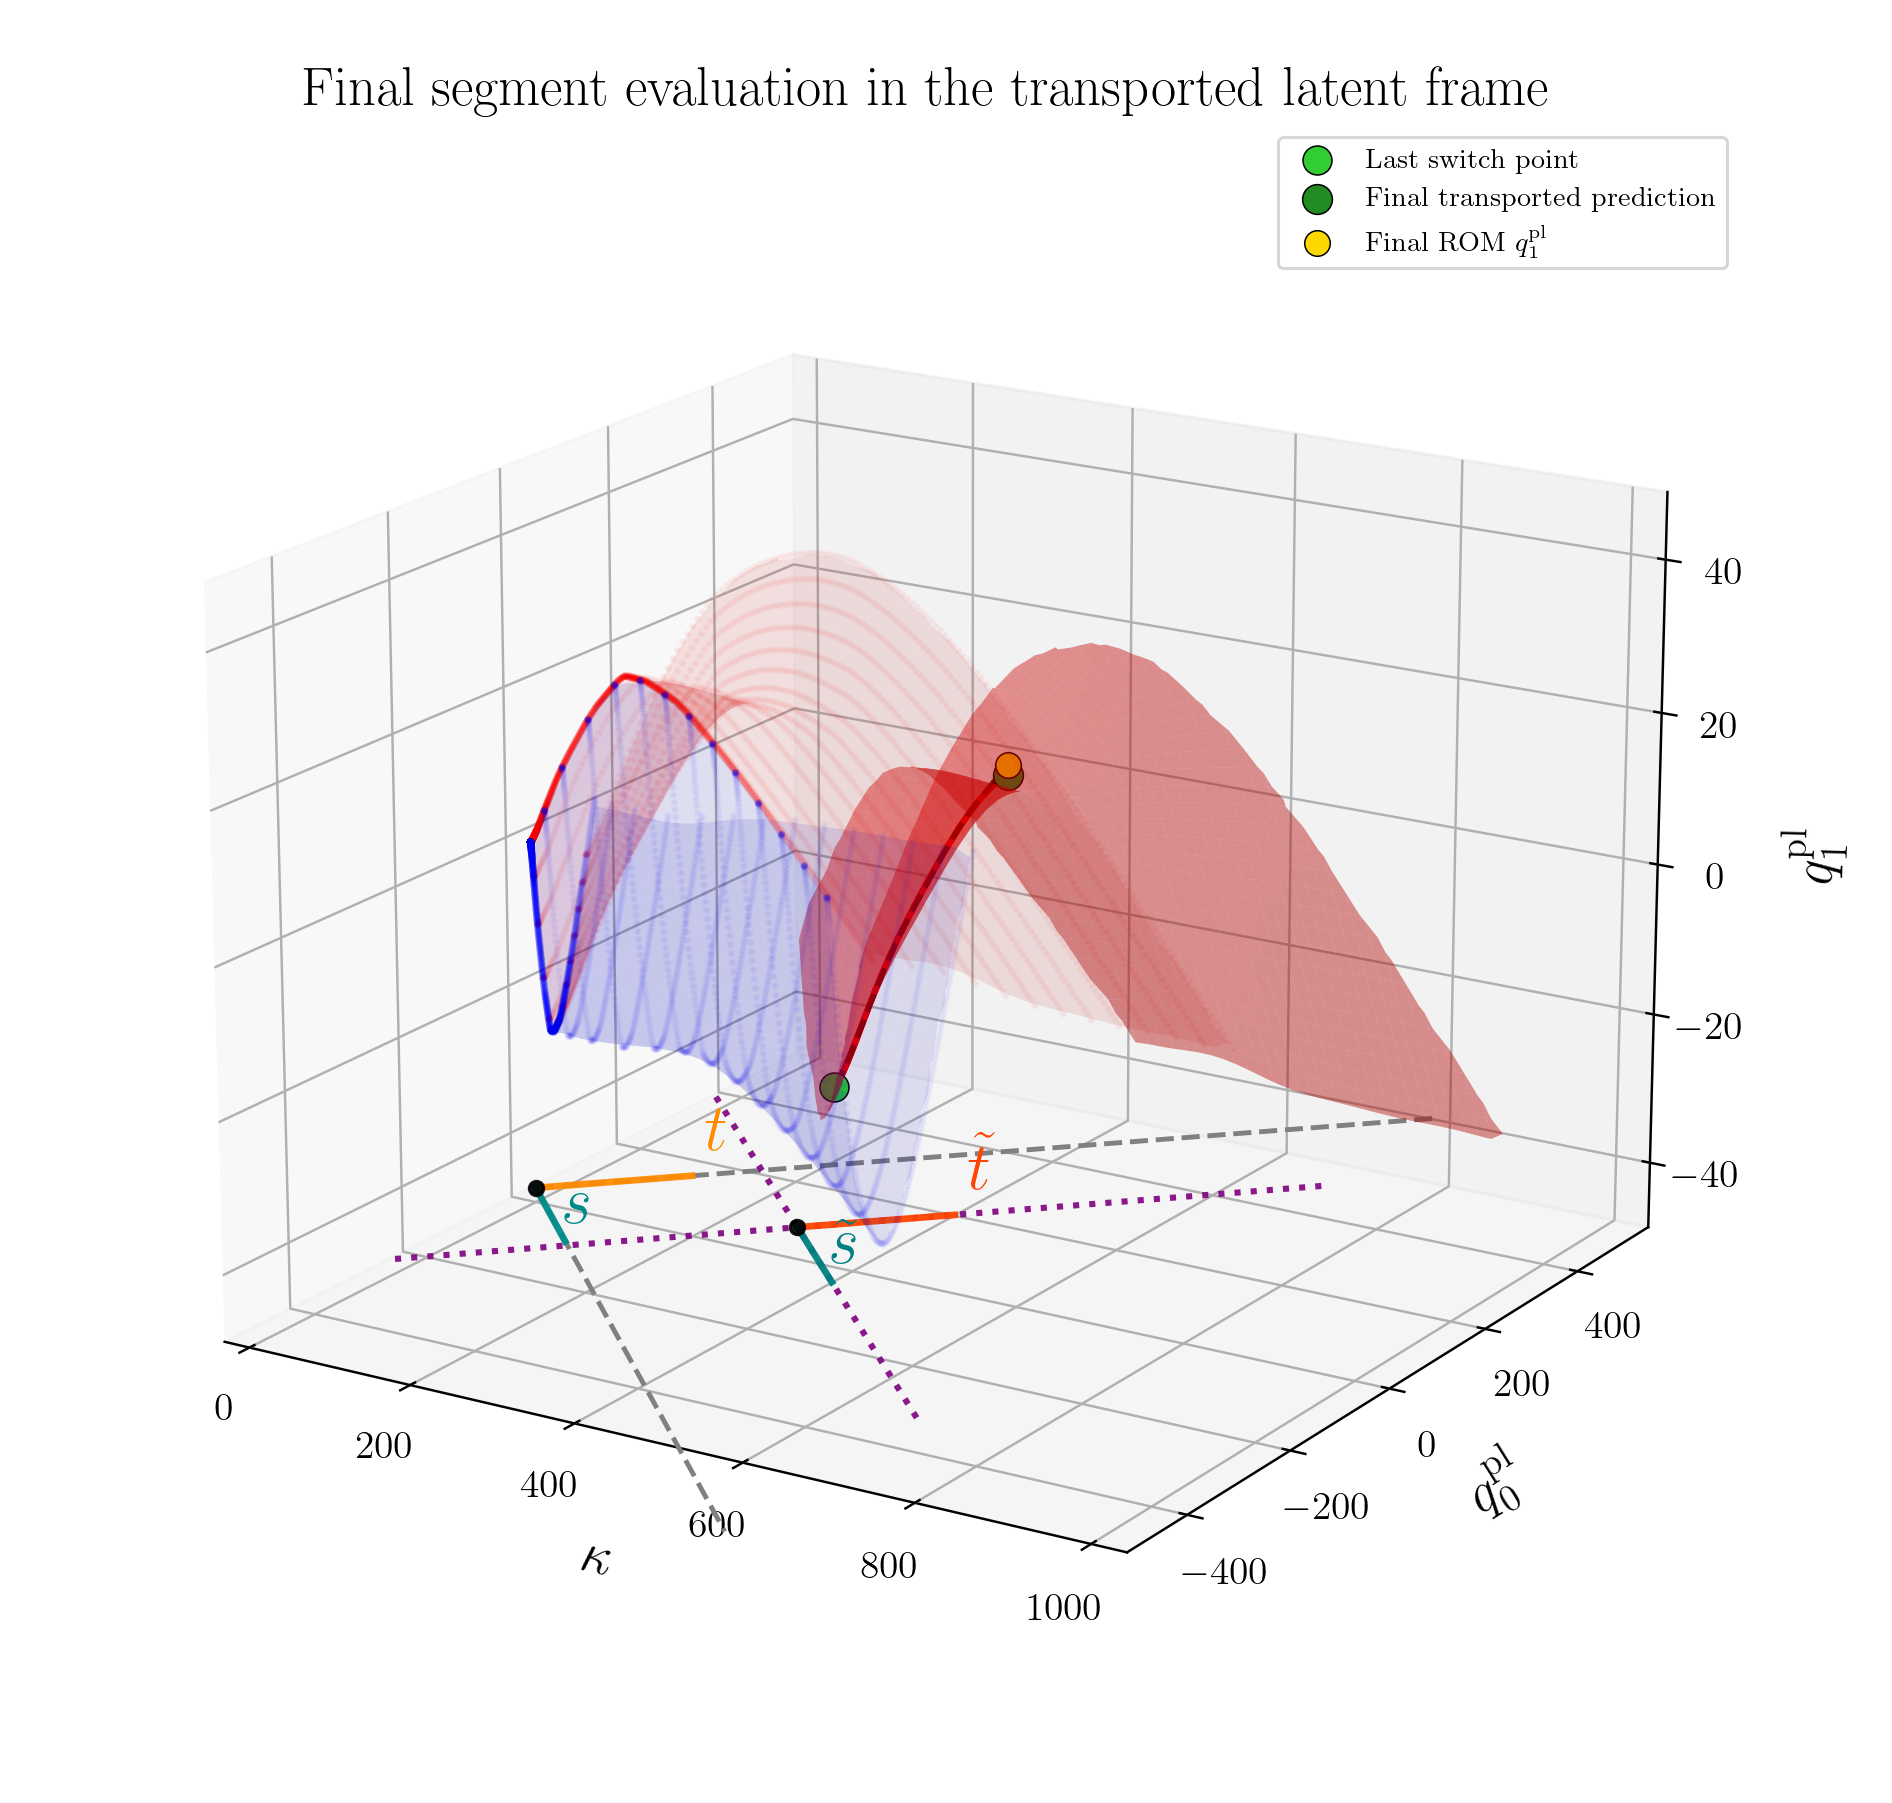
\includegraphics[width=\textwidth]{two_surface_switch_with_boundary_projection_transport/final_segment_transport_view1.png}
\caption{Final evaluation in latent space.}
\end{subfigure}
\caption{Final segment evaluation after the last switch. The point is evaluated on the transported red branch using the final transport state.}
\label{fig:tutorial_final_segment}
\end{figure}

\subsection{What the worked example shows}

The numerical example confirms the logic of the method:

\begin{itemize}
\item At each switch, the current point is first related to the newly active branch through a boundary anchor.
\item The whole latent frame is then translated in-plane so that the anchor reaches the switching point.
\item The newly activated branch is vertically re-anchored so that its value matches the ROM target coordinate at that point.
\item Between switches, the transport state remains fixed and the active branch is evaluated in the transported frame.
\end{itemize}

Seen this way, the transported surrogate is not mysterious. It is a fixed pair of offline branchwise surfaces together with an online bookkeeping rule that updates where those surfaces are evaluated and how they are vertically aligned with the trajectory.

% ============================================================
% Algorithm 1: Online-consistent projection-transport
% ============================================================
\begin{algorithm}[H]
\caption{Branchwise Projection-Transport in $(s,t)$ Coordinates}
\begin{algorithmic}[1]

\State \textbf{Coordinate map}
\[
t_k=\frac{\kappa_k+q_{0,k}^{\mathrm{pl}}}{2},
\qquad
s_k=\frac{\kappa_k-q_{0,k}^{\mathrm{pl}}}{2}
\]

\State \textbf{Branch rule from the loading increment}
\[
\beta_k=
\begin{cases}
+,& \Delta\varepsilon_{xx,k}>0,\\
-,& \Delta\varepsilon_{xx,k}<0
\end{cases}
\]

\State \textbf{State variables}
\[
\tilde s,\tilde t,\ \delta q^+,\delta q^-
\]
\Statex \hspace{\algorithmicindent} where $(\tilde s,\tilde t)$ is the transported frame and $\delta q^\pm$ are branchwise vertical offsets

\State \textbf{Boundary projections}
\[
P_+(s,t)=(\tilde s,t),\qquad
P_-(s,t)=(s,\tilde t)
\]

\State \textbf{Initialize}
\[
(\tilde s,\tilde t)\gets(0,0),\qquad
\delta q^+\gets0,\quad \delta q^-\gets0,\qquad
\beta\gets\beta_{k_0}
\]

\For{$k=k_0,\dots,N$}
    \State $C_k=(s_k,t_k)$
    \State Evaluate the current transported branch at the current point:
    \[
    q_k^C=\mathcal N^\beta(t_k-\tilde t,\ s_k-\tilde s)+\delta q^\beta
    \]

    \If{$\beta_k\neq\beta$}
        \State $\beta\gets\beta_k$

        \State Project the switching point to the boundary of the newly active branch:
        \[
        B_k=(s_b,t_b)=
        \begin{cases}
        P_+(C_k), & \beta=+,\\
        P_-(C_k), & \beta=-
        \end{cases}
        \]

        \State Evaluate the newly active transported branch at the boundary anchor:
        \[
        q_k^B=\mathcal N^\beta(t_b-\tilde t,\ s_b-\tilde s)+\delta q^\beta
        \]

        \State Update the transported frame cumulatively:
        \[
        \tilde s\gets\tilde s+(s_k-s_b),\qquad
        \tilde t\gets\tilde t+(t_k-t_b)
        \]

        \State Vertically re-anchor only the newly active branch by continuity:
        \[
        \delta q^\beta\gets\delta q^\beta+(q_k^C-q_k^B)
        \]
    \EndIf

    \State Final transported prediction:
    \[
    q_k=\mathcal N^\beta(t_k-\tilde t,\ s_k-\tilde s)+\delta q^\beta
    \]
\EndFor

\end{algorithmic}
\end{algorithm}


% ============================================================
% Algorithm 2: Incremental Differential Transport (clean form)
% ============================================================
\begin{algorithm}[H]
\caption{Incremental Differential Branchwise Evolution in $(s,t)$ Coordinates}
\begin{algorithmic}[1]

\State \textbf{Given path variables}
\[
q_{M,k},\ \beta_k\in\{+,-\},\qquad k=0,\dots,N
\]

\State \textbf{Accumulated measure}
\[
\lambda_{k+1}=|q_{M,k+1}-q_{M,k}|,\qquad
\kappa_{k+1}=\kappa_k+\lambda_{k+1}
\]

\State \textbf{Coordinate map}
\[
t_k=\frac{\kappa_k+q_{M,k}}{2},\qquad
s_k=\frac{\kappa_k-q_{M,k}}{2}
\]

\State \textbf{Direction map (one per branch)}
\[
D_+,D_-\in\{t,s\}
\]
\Statex \hspace{\algorithmicindent} (identified from path kinematics or prescribed)

\State \textbf{State variables}
\[
\bar s,\bar t,\ q_k,\ \hat\beta
\]

\State \textbf{Initialize}
\[
(\bar s,\bar t)\gets(0,0),\qquad
\hat\beta\gets\beta_{k_0},\qquad
q_0\gets q_0^{\text{init}}
\]

\For{$k=0,\dots,N-1$}
    \State $\lambda_{k+1}=|q_{M,k+1}-q_{M,k}|$
    \If{$\lambda_{k+1}\le\varepsilon_\lambda$}
        \State $q_{k+1}\gets q_k,\ \hat\beta\gets\hat\beta$
        \State \textbf{continue}
    \EndIf

    \State $\chi_{k+1}=\dfrac{|\beta_{k+1}-\hat\beta|}{2}$  \Comment{switch detector}
    \State
    \[
    D=
    \begin{cases}
    D_+, & \beta_{k+1}=+\\
    D_-, & \beta_{k+1}=-
    \end{cases}
    \]

    \State Frame update at switching:
    \[
    (\bar s,\bar t)\gets
    \begin{cases}
    (\bar s,\ \bar t+\chi_{k+1}(t_{k+1}-\bar t)), & D=t\\
    (\bar s+\chi_{k+1}(s_{k+1}-\bar s),\ \bar t), & D=s
    \end{cases}
    \]

    \State Local coordinates at step $k$:
    \[
    \hat s_k=s_k-\bar s,\qquad
    \hat t_k=t_k-\bar t
    \]

    \State Directional tangents:
    \[
    G_t^\pm=\partial_t\mathcal N^\pm(\hat t_k,\hat s_k),\qquad
    G_s^\pm=\partial_s\mathcal N^\pm(\hat t_k,\hat s_k)
    \]

    \State Increments:
    \[
    \Delta t_k=t_{k+1}-t_k,\qquad
    \Delta s_k=s_{k+1}-s_k
    \]

    \State Differential update:
    \[
    \Delta q_k=
    \begin{cases}
    G_t^+\,\Delta t_k, & \beta_{k+1}=+,\ D_+=t\\
    G_s^+\,\Delta s_k, & \beta_{k+1}=+,\ D_+=s\\
    G_t^-\,\Delta t_k, & \beta_{k+1}=-,\ D_-=t\\
    G_s^-\,\Delta s_k, & \beta_{k+1}=-,\ D_-=s
    \end{cases}
    \]
    \[
    q_{k+1}=q_k+\Delta q_k,\qquad
    \hat\beta\gets\beta_{k+1}
    \]
\EndFor

\end{algorithmic}
\end{algorithm}


% ============================================================
% Algorithm 3: Compact Incremental Transport (q_{0}^{pl} nomenclature)
% ============================================================
\newpage
\begin{algorithm}[H]
\caption{Compact Incremental Branchwise Evolution in $(s,t)$ Coordinates}
\begin{algorithmic}[1]

\State \textbf{Coordinate map}
\[
t_k=\frac{\kappa_k+q_{0,k}^{\mathrm{pl}}}{2},
\qquad
s_k=\frac{\kappa_k-q_{0,k}^{\mathrm{pl}}}{2}
\]

\State \textbf{Branch rule from loading increment}
\[
\beta_k=
\begin{cases}
+,& \Delta\varepsilon_{xx,k}>0,\\
-,& \Delta\varepsilon_{xx,k}<0
\end{cases}
\]

\State \textbf{Accumulated measure from master coordinate}
\[
\lambda_{k+1}=|q_{0,k+1}^{\mathrm{pl}}-q_{0,k}^{\mathrm{pl}}|,
\qquad
\kappa_{k+1}=\kappa_k+\lambda_{k+1}
\]

\State \textbf{Direction map (one per branch)}
\[
D_+,D_-\in\{t,s\}
\]

\State \textbf{State variables}
\[
\bar s,\bar t,\ q_k,\ \hat\beta
\]

\State \textbf{Compact coefficient}
\[
c_-\in\mathbb{R}
\]
\Statex \hspace{\algorithmicindent} typically $c_-=+1$

\State \textbf{Initialize}
\[
(\bar s,\bar t)\gets(0,0),\qquad
\hat\beta\gets\beta_{k_0},\qquad
q_{k_0}\gets q_{k_0}^{\mathrm{init}}
\]

\For{$k=k_0,\dots,N-1$}
    \State $\lambda_{k+1}=|q_{0,k+1}^{\mathrm{pl}}-q_{0,k}^{\mathrm{pl}}|$
    \If{$\lambda_{k+1}\le\varepsilon_\lambda$}
        \State $q_{k+1}\gets q_k$
        \State \textbf{continue}
    \EndIf

    \State $\chi_{k+1}=\dfrac{|\beta_{k+1}-\hat\beta|}{2}$

    \State
    \[
    D=
    \begin{cases}
    D_+, & \beta_{k+1}=+\\
    D_-, & \beta_{k+1}=-
    \end{cases}
    \]

    \State Direction-aware compact frame update at switching:
    \[
    (\bar s,\bar t)\gets
    \begin{cases}
    (\bar s,\ \bar t+\chi_{k+1}(t_k-\bar t)), & D=t\\
    (\bar s+\chi_{k+1}(s_k-\bar s),\ \bar t), & D=s
    \end{cases}
    \]

    \State Local coordinates at step $k$:
    \[
    \hat s_k=s_k-\bar s,\qquad
    \hat t_k=t_k-\bar t
    \]

    \State Directional tangents:
    \[
    G_t^\pm=\partial_t\mathcal N^\pm(\hat t_k,\hat s_k),\qquad
    G_s^\pm=\partial_s\mathcal N^\pm(\hat t_k,\hat s_k)
    \]

    \State Active branch tangents:
    \[
    G_+^{\mathrm{act}}=
    \begin{cases}
    G_t^+, & D_+=t\\
    G_s^+, & D_+=s
    \end{cases},
    \qquad
    G_-^{\mathrm{act}}=
    \begin{cases}
    G_t^-, & D_-=t\\
    G_s^-, & D_-=s
    \end{cases}
    \]

    \State Branch indicators:
    \[
    I_+^{k+1}=\frac{1+\beta_{k+1}}{2},\qquad
    I_-^{k+1}=\frac{1-\beta_{k+1}}{2}
    \]

    \State Compact update:
    \[
    q_{k+1}
    =
    q_k
    +
    I_+^{k+1}G_+^{\mathrm{act}}\,\lambda_{k+1}
    +
    c_-\,I_-^{k+1}G_-^{\mathrm{act}}\,\lambda_{k+1}
    \]

    \State $\hat\beta\gets\beta_{k+1}$
\EndFor

\end{algorithmic}
\end{algorithm}



\newpage
\noindent\textbf{Algorithm: Incremental associative plasticity in generalized variables}

\begin{algorithmic}[1]

\State \textbf{Generalized variables:}
\[
\mathcal S := \{\sigma,\eta\},
\qquad
\mathcal E^{pl} := \{\varepsilon^p,\xi\}
\]
\Statex \hspace{\algorithmicindent}
$\triangleright$ $\sigma$ and $\eta$ are the thermodynamic forces conjugate to
$\varepsilon^p$ and $\xi$, respectively

\State \textbf{Free energy:}
\[
\Psi(\varepsilon,\varepsilon^p,\xi)
=
\frac12 (\varepsilon-\varepsilon^p):\mathbf C:(\varepsilon-\varepsilon^p)
+
\Psi_{\mathrm{hard}}(\xi)
\]
\Statex \hspace{\algorithmicindent}
$\triangleright$ for instance, a simple quadratic hardening law is
\[
\Psi_{\mathrm{hard}}(\xi)=\frac12\,H\,\xi^2
\]

\State \textbf{Constitutive relations:}
\[
\sigma
=
\frac{\partial \Psi}{\partial \varepsilon}
=
\mathbf C:(\varepsilon-\varepsilon^p)
\]
\[
\eta
=
-
\frac{\partial \Psi}{\partial \xi}
\]
\Statex \hspace{\algorithmicindent}
$\triangleright$ equivalently, $\sigma = -\dfrac{\partial \Psi}{\partial \varepsilon^p}$

\State \textbf{Yield function:}
\[
f(\sigma,\eta)\le 0
\]

\State \textbf{Associative flow rule:}
\[
\dot{\mathcal E}^{pl}
=
\dot\lambda\,
\frac{\partial f}{\partial \mathcal S}
\]
that is,
\[
\dot{\varepsilon}^p = \dot\lambda\,\frac{\partial f}{\partial \sigma},
\qquad
\dot{\xi} = \dot\lambda\,\frac{\partial f}{\partial \eta}
\]

\State \textbf{KKT conditions:}
\[
\Delta\lambda \ge 0,
\qquad
f(\sigma,\eta)\le 0,
\qquad
\Delta\lambda\,f(\sigma,\eta)=0
\]

\State \textbf{Known state at step $n$:}
\[
\varepsilon_n^p,\qquad \xi_n
\]

\For{each load step $n+1$}

    \State \textbf{Given input strain:}
    \[
    \varepsilon_{n+1}
    \]

    \State \textbf{Trial elastic strain:}
    \[
    \varepsilon_{n+1}^{e,tr}
    =
    \varepsilon_{n+1}-\varepsilon_n^p
    \]

    \State \textbf{Trial thermodynamic forces:}
    \[
    \sigma_{n+1}^{tr}
    =
    \mathbf C:\varepsilon_{n+1}^{e,tr}
    =
    \frac{\partial\Psi}{\partial\varepsilon}
    (\varepsilon_{n+1},\varepsilon_n^p,\xi_n)
    \]
    \[
    \eta_{n+1}^{tr}
    =
    -
    \frac{\partial\Psi}{\partial\xi}
    (\varepsilon_{n+1},\varepsilon_n^p,\xi_n)
    \]

    \State \textbf{Trial admissibility check:}
    \[
    f_{n+1}^{tr}
    =
    f(\sigma_{n+1}^{tr},\eta_{n+1}^{tr})
    \]

    \If{$f_{n+1}^{tr}\le 0$}
        \State \textbf{Elastic step:}
        \[
        \sigma_{n+1}\gets \sigma_{n+1}^{tr},
        \qquad
        \eta_{n+1}\gets \eta_{n+1}^{tr}
        \]
        \[
        \varepsilon_{n+1}^p\gets \varepsilon_n^p,
        \qquad
        \xi_{n+1}\gets \xi_n
        \]
    \Else
        \State \textbf{Plastic correction (return mapping):}

        \State Solve for $\Delta\lambda_{n+1}>0$ such that the consistency condition holds:
        \[
        f(\sigma_{n+1},\eta_{n+1})=0
        \]

        \State Update generalized plastic variables:
        \[
        \varepsilon_{n+1}^p
        =
        \varepsilon_n^p
        +
        \Delta\lambda_{n+1}\,
        \frac{\partial f}{\partial \sigma}(\sigma_{n+1},\eta_{n+1})
        \]
        \[
        \xi_{n+1}
        =
        \xi_n
        +
        \Delta\lambda_{n+1}\,
        \frac{\partial f}{\partial \eta}(\sigma_{n+1},\eta_{n+1})
        \]

        \State Recompute elastic strain:
        \[
        \varepsilon_{n+1}^e
        =
        \varepsilon_{n+1}-\varepsilon_{n+1}^p
        \]

        \State Recompute thermodynamic forces:
        \[
        \sigma_{n+1}
        =
        \mathbf C:\varepsilon_{n+1}^e
        =
        \frac{\partial\Psi}{\partial\varepsilon}
        (\varepsilon_{n+1},\varepsilon_{n+1}^p,\xi_{n+1})
        \]
        \[
        \eta_{n+1}
        =
        -
        \frac{\partial\Psi}{\partial\xi}
        (\varepsilon_{n+1},\varepsilon_{n+1}^p,\xi_{n+1})
        \]
    \EndIf

\EndFor

\end{algorithmic}

\newpage
\noindent\textbf{Algorithm: Reduced incremental associative plasticity in generalized variables}

\begin{algorithmic}[1]

\State \textbf{Generalized variables:}
\[
\mathcal S := \{\sigma,\eta\},
\qquad
\mathcal E^{pl} := \{\varepsilon^p,\xi\}
\]
\Statex \hspace{\algorithmicindent}
$\triangleright$ $\sigma$ and $\eta$ are the thermodynamic forces conjugate to
$\varepsilon^p$ and $\xi$, respectively

\State \textbf{Snapshot-based reduced representations:}
\[
\mathcal S \approx \Phi_S q_S,
\qquad
\mathcal E^{pl} \approx \Phi_E q_E
\]
\Statex \hspace{\algorithmicindent}
$\triangleright$ $\Phi_S$ and $\Phi_E$ are obtained from two POD/SVD decompositions of force and internal-variable snapshots

\State \textbf{Reduced generalized variables:}
\[
\mathcal S_r := \{\sigma_r,\eta_r\} := \Phi_S q_S,
\qquad
\mathcal E_r^{pl} := \{\varepsilon_r^p,\xi_r\} := \Phi_E q_E
\]

\State \textbf{Free energy:}
\[
\Psi(\varepsilon,\varepsilon^p,\xi)
=
\frac12 (\varepsilon-\varepsilon^p):\mathbf C:(\varepsilon-\varepsilon^p)
+
\Psi_{\mathrm{hard}}(\xi)
\]
\Statex \hspace{\algorithmicindent}
$\triangleright$ for instance, a simple quadratic hardening law is
\[
\Psi_{\mathrm{hard}}(\xi)=\frac12\,H\,\xi^2
\]

\State \textbf{Projected reduced constitutive relations:}
\[
\mathcal S_r(\varepsilon,q_E)
:=
\Phi_S^T\,\mathcal S(\varepsilon,\Phi_E q_E)
\]
that is,
\[
q_S(\varepsilon,q_E)
=
\Phi_S^T
\begin{Bmatrix}
\sigma(\varepsilon,\Phi_E q_E) \\
\eta(\varepsilon,\Phi_E q_E)
\end{Bmatrix}
\]
\Statex \hspace{\algorithmicindent}
$\triangleright$ careful: unlike the full model, the reduced forces are not independent variables; they are induced from the reduced internal state

\State \textbf{Reduced yield function:}
\[
f_r(q_S)\le 0,
\qquad
f_r(q_S):=f(\Phi_S q_S)
\]
\Statex \hspace{\algorithmicindent}
$\triangleright$ simpler choice; more elaborate variants may use $f_r(q_S,q_E)$

\State \textbf{Reduced associative flow rule:}
\[
\dot q_E
=
\dot\lambda_r\,N_r
\]
with
\[
N_r \approx \Phi_E^T \dot{\mathcal E}^{pl}
\]
or, equivalently, in algorithmic form,
\[
q_E^{n+1}=q_E^n+\Delta\lambda_{n+1}^r\,N_{r,n+1}
\]
\Statex \hspace{\algorithmicindent}
$\triangleright$ this is the least canonical part of the reduced model; $N_r$ must be defined by projection or learned consistently from data

\State \textbf{Reduced KKT conditions:}
\[
\Delta\lambda^r \ge 0,
\qquad
f_r(q_S)\le 0,
\qquad
\Delta\lambda^r\,f_r(q_S)=0
\]

\State \textbf{Known reduced state at step $n$:}
\[
q_{E,n}
\]
\Statex \hspace{\algorithmicindent}
$\triangleright$ equivalently, $\mathcal E_{r,n}^{pl}=\Phi_E q_{E,n}$

\For{each load step $n+1$}

    \State \textbf{Given input strain:}
    \[
    \varepsilon_{n+1}
    \]

    \State \textbf{Trial reduced internal state:}
    \[
    q_{E,n+1}^{tr}=q_{E,n}
    \]

    \State \textbf{Trial reconstructed internal variables:}
    \[
    \mathcal E_{r,n+1}^{pl,tr}
    =
    \Phi_E q_{E,n}
    =
    \{\varepsilon_{r,n}^{p},\xi_{r,n}\}
    \]

    \State \textbf{Trial reduced thermodynamic forces:}
    \[
    q_{S,n+1}^{tr}
    =
    \Phi_S^T\,\mathcal S(\varepsilon_{n+1},\Phi_E q_{E,n})
    \]
    that is,
    \[
    \mathcal S_{r,n+1}^{tr}
    =
    \Phi_S q_{S,n+1}^{tr}
    =
    \{\sigma_{r,n+1}^{tr},\eta_{r,n+1}^{tr}\}
    \]

    \State \textbf{Trial reduced admissibility check:}
    \[
    f_{r,n+1}^{tr}
    =
    f_r(q_{S,n+1}^{tr})
    =
    f(\Phi_S q_{S,n+1}^{tr})
    \]

    \If{$f_{r,n+1}^{tr}\le 0$}
        \State \textbf{Elastic step:}
        \[
        q_{S,n+1}\gets q_{S,n+1}^{tr}
        \]
        \[
        q_{E,n+1}\gets q_{E,n}
        \]
        \Statex \hspace{\algorithmicindent}
        $\triangleright$ equivalently,
        \[
        \mathcal S_{r,n+1}\gets \mathcal S_{r,n+1}^{tr},
        \qquad
        \mathcal E_{r,n+1}^{pl}\gets \mathcal E_{r,n}^{pl}
        \]
    \Else
        \State \textbf{Plastic correction (reduced return mapping):}

        \State Solve for $\Delta\lambda_{n+1}^r>0$ such that the reduced consistency condition holds:
        \[
        f_r(q_{S,n+1})=0
        \]

        \State Update reduced generalized plastic variables:
        \[
        q_{E,n+1}
        =
        q_{E,n}
        +
        \Delta\lambda_{n+1}^r\,N_{r,n+1}
        \]
        \Statex \hspace{\algorithmicindent}
        $\triangleright$ equivalently,
        \[
        \mathcal E_{r,n+1}^{pl}
        =
        \Phi_E q_{E,n+1}
        =
        \{\varepsilon_{r,n+1}^{p},\xi_{r,n+1}\}
        \]

        \State Recompute reduced thermodynamic forces:
        \[
        q_{S,n+1}
        =
        \Phi_S^T\,\mathcal S(\varepsilon_{n+1},\Phi_E q_{E,n+1})
        \]
        that is,
        \[
        \mathcal S_{r,n+1}
        =
        \Phi_S q_{S,n+1}
        =
        \{\sigma_{r,n+1},\eta_{r,n+1}\}
        \]

        \Statex \hspace{\algorithmicindent}
        $\triangleright$ simpler but weaker alternative: learn a direct map
        \[
        q_{S,n+1}=\mathcal G_r(\varepsilon_{n+1},q_{E,n+1})
        \]
        instead of computing it by projection of the constitutive response
    \EndIf

\EndFor

\end{algorithmic}
\end{document}